
\documentclass[a4paper,12pt,twoside,titlepage]{book}

\usepackage{scaladoc}
\usepackage{fleqn}
\usepackage{modefs}
\usepackage{math}
\usepackage{scaladefs}
\renewcommand{\todo}[1]{}



\ifpdf
    \pdfinfo {
        /Author   (Martin Odersky)
        /Title    (Programming in Scala)
        /Keywords (Scala)
        /Subject  ()
        /Creator  (TeX)
        /Producer (PDFLaTeX)
    }
\fi

\renewcommand{\doctitle}{Programming in Scala\\[33mm]\ }
\renewcommand{\docauthor}{Martin Odersky\\[53mm]\ }

\begin{document}

\frontmatter
\makedoctitle
\clearemptydoublepage
\tableofcontents
\mainmatter
\sloppy

\part{Rationale}


There are hundreds of programming languages in active use, and many
more are being designed each year. It is therefore hard to justify the
development of yet another language. Nevertheless, this is what we
attempt to do here.  Our argument is based on two claims:
\begin{itemize}
\item[] {\em Claim 1:} The raise in importance of web services and
other distributed software is a fundamental paradigm
shift in programming. It is comparable in scale to the shift 20 years ago
from character-oriented to graphical user interfaces.
\item[] {\em Claim 2:} That paradigm shift will provide demand
for new programming languages, just as graphical user interfaces
promoted the adoption of object-oriented languages.
\end{itemize}
For the last 20 years, the most common programming model was
object-oriented: System components are objects, and computation is
done by method calls.  Methods themselves take object references as
parameters. Remote method calls let one extend this programming model
to distributed systems. The problem of this model is that it does not
scale up very well to wide-scale networks where messages can be
delayed and components may fail. Web services address the message
delay problem by increasing granularity, using method calls with
larger, structured arguments, such as XML trees.  They address the
failure problem by using transparent replication and avoiding server
state.  Conceptually, they are {\em tree transformers} that consume
incoming message documents and produce outgoing ones.  \comment{ To
back up the first claim, one observes that web services and other
distributed software increasingly tend to communicate using structured
or semi-structured data. A typical example is the use of XML to
describe data managed by applications as well as the messages between
applications. This tends to affect the role of a program in a
fundamental way. Previously, programs could be seen as objects that
reacted to method calls and in turn called methods of other
objects. Some of these method calls might originate from users while
others might originate from other computers via remote invocations.
These method calls have simple unstructured parameters or object
references as arguments.  Web services, on the other hand, communicate
with each other by transmitting asynchronous messages that carry
structured documents, usually in XML format. Programs then
conceptually become {\em tree transformers} that consume incoming
message documents and produce outgoing ones.  }

Why should this have an effect on programming languages? There are at
least two reasons: First, today's object-oriented languages are not
very good at analyzing and transforming XML trees. Because such trees
usually contain data but no methods, they have to be decomposed and
constructed from the ``outside'', that is from code which is external
to the tree definition itself. In an object-oriented language, the
ways of doing so are limited. The most common solution \cite{w3c:dom} is
to represent trees in a generic way, where all tree nodes are values
of a common type.  This makes it easy to write generic traversal
functions, but forces applications to operate on a very low conceptual
level, which often loses important semantic distinctions present in
the XML data.  More semantic precision is obtained if different
internal types model different kinds of nodes.  But then tree
decompositions require the use of run-time type tests and type casts
to adapt the treatment to the kind of node encountered. Such type
tests and type casts are generally not considered good object-oriented
style. They are rarely efficient, nor easy to use.


By contrast, tree transformation is the natural domain of functional
languages. Their algebraic data types, pattern matching and
higher-order functions make these languages ideal for the task. It's
no wonder, then, that specialized languages for transforming XML data
such as XSLT are functional.

Another reason why functional language constructs are attractive for
web-services is that mutable state is problematic in this setting.
Components with mutable state are harder to replicate or to restore
after a failure. Data with mutable state is harder to cache than
immutable data. Functional language constructs make it relatively easy
to construct components without mutable state.

Many web services are constructed by combining different languages.
For instance, a service might use XSLT to handle document
transformation, XQuery for database access, and Java for the
``business logic''.  The downside of this approach is that the
necessary amount of cross-language glue can make applications
cumbersome to write, verify, and maintain. A particular problem is
that cross-language interfaces are usually not statically typed.
Hence, the benefits of a static type system are missing where they are
needed most -- at the join points of components written in different
paradigms.  

Conceivably, the glue problem could be addressed by a ``multi-paradigm''
language that would express object-oriented, concurrent, as well
as functional aspects of an application.  But one needs to be careful
not to simply replace cross-language glue by awkward interfaces
between different paradigms within the language itself.  Ideally, one
would hope for a fusion which unifies concepts found in different
paradigms instead of an agglutination, which merely includes them side
by side.  This fusion is what we try to achieve with Scala
\footnote{Scala stands for ``Scalable Language''. The term means
  ``Stairway'' in Italian}.

Scala is both an object-oriented and functional language.  It is a
pure object-oriented language in the sense that every value is an
object. Types and behavior of objects are described by
classes. Classes can be composed using mixin composition.  Scala is
designed to work seamlessly with mainstream object-oriented languages,
in particular Java and C\#.

Scala is also a functional language in the sense that every function
is a value. Nesting of function definitions and higher-order functions
are naturally supported. Scala also supports a general notion of
pattern matching which can model the algebraic types used in many
functional languages. Furthermore, this notion of pattern matching
naturally extends to the processing of XML data.

The design of Scala is driven by the desire to unify object-oriented
and functional elements. Here are three examples how this is achieved:
\begin{itemize}
\item
Since every function is a value and every value is an object, it
follows that every function in Scala is an object. Indeed, there is a
root class for functions which is specialized in the Scala standard
library to data structures such as arrays and hash tables.
\item
Data structures in many functional languages are defined using
algebraic data types. They are decomposed using pattern matching.
Object-oriented languages, on the other hand, describe data with class
hierarchies. Algebraic data types are usually closed, in that the
range of alternatives of a type is fixed when the type is defined.  By
contrast, class hierarchies can be extended by adding new leaf
classes.  Scala adopts the object-oriented class hierarchy scheme for
data definitions, but allows pattern matching against values coming
from a whole class hierarchy, not just values of a single type.
This can express both closed and extensible data types, and also
provides a convenient way to exploit run-time type information in
cases where static typing is too restrictive.
\item
Module systems of functional languages such as SML or Caml excel in
abstraction; they allow very precise control over visibility of names
and types, including the ability to partially abstract over types.  By
contrast, object-oriented languages excel in composition; they offer
several composition mechanisms lacking in module systems, including
inheritance and unlimited recursion between objects and classes.
Scala unifies the notions of object and module, of module signature
and interface, as well as of functor and class. This combines the
abstraction facilities of functional module systems with the
composition constructs of object-oriented languages. The unification
is made possible by means of a new type system based on path-dependent
types \cite{odersky-et-al:fool10}.
\end{itemize}
There are several other languages that try to bridge the gap between
the functional and object oriented
paradigms. Smalltalk\cite{goldberg-robson:smalltalk-language},
Python\cite{rossum:python}, or Ruby\cite{matsumtoto:ruby} come to
mind. Unlike these languages, Scala has an advanced static type
system, which contains several innovative constructs.  This aspect
makes the Scala definition a bit more complicated than those of the
languages above. On the other hand, Scala enjoys the robustness,
safety and scalability benefits of strong static typing. Furthermore,
Scala incorporates recent advances in type inference, so that
excessive type annotations in user programs can usually be avoided.

% rest of this report is structured as follows. Chapters
%\ref{sec:simple-examples} to \ref{sec:concurrency} give an informal overview of
%Scala by means of a sequence of program examples.  The remaining
%chapters contain the language definition. The definition is formulated
%in prose but tries to be precise.



\paragraph{Acknowledgments}
Many people have contributed to the definition and implementation of
the Scala language and to parts of this book. First of all, I would
like to thank the Scala team at EPFL consisting of Philippe Altherr,
Vincent Cremet, Burak Emir, St\'ephane Micheloud, Nikolay Mihaylov,
Michel Schinz, Erik Stenman, and Matthias Zenger. They put a lot of
effort in the Scala compiler, tools, and documentation and have
contributed in an essential way to the specification of the Scala
language through many observations, clever suggestions, and
discussions. Members of the team have also contributed examples in
this book, as well as parts of the specification. Phil Bagwell, Gilad
Bracha, Erik Ernst, Erik Mejer, Benjamin Pierce, Enno Runne, and Phil
Wadler have given very useful feedback on the Scala design. 

The documentation ows a great debt to Abelson's and Sussman's
wonderful book ``Structure and Interpretation of Computer
Programs''\cite{abelson-sussman:structure}. I have adapted several of
their examples and exercises in the ``Scala By Example'' part of this
book. Of course, the working language has in each case been changed
from Scheme to Scala. Furthermore, the examples make use of Scala's
object-oriented constructs where appropriate.

\part{Scala by Example}

Scala is a programming language that fuses elements from
object-oriented and functional programming. This part introduces Scala
in an informal way, through a sequence of examples.

Chapters~\ref{chap:example-one} and \ref{chap:example-auction}
highlight some of the features that make Scala interesting. The
following chapters introduce the language constructs of Scala in a
more thorough way, starting with simple expressions and functions, and
working up through objects and classes, lists and streams, mutable
state, pattern matching to more complete examples that show
interesting programming techniques. The present informal exposition is
complemented by the Scala Language Reference Manual which specifies
Scala in a more detailed and precise way.

\def\exercise{
   \def\theresult{Exercise~\thesection.\arabic{result}}
   \refstepcounter{result}
   \trivlist\item[\hskip
   \labelsep{\bf \theresult}]}
\def\endexercise{\endtrivlist}
 
\newcommand{\rewriteby}[1]{\mbox{\tab\tab\rm(#1)}}

\chapter{\label{chap:example-one}A First Example}

As a first example, here is an implementation of Quicksort in Scala.

\begin{lstlisting}
def sort(xs: Array[Int]) {
  def swap(i: Int, j: Int) {
    val t = xs(i); xs(i) = xs(j); xs(j) = t
  }
  def sort1(l: Int, r: Int) {
    val pivot = xs((l + r) / 2)
    var i = l; var j = r
    while (i <= j) {
      while (xs(i) < pivot) i += 1
      while (xs(j) > pivot) j -= 1
      if (i <= j) { 
        swap(i, j)
        i += 1
        j -= 1
      }
    } 
    if (l < j) sort1(l, j)
    if (j < r) sort1(i, r)
  }
  sort1(0, xs.length - 1)
}
\end{lstlisting}

The implementation looks quite similar to what one would write in Java
or C.  We use the same operators and similar control structures.
There are also some minor syntactical differences. In particular:
\begin{itemize}
\item
Definitions start with a reserved word. Function definitions start
with \code{def}, variable definitions start with \code{var} and
definitions of values (i.e. read only variables) start with \code{val}.
\item
The declared type of a symbol is given after the symbol and a colon.
The declared type can often be omitted, because the compiler can infer
it from the context.
\item
Array types are written \code{Array[T]} rather than \code{T[]}, 
and array selections are written \code{a(i)} rather than \code{a[i]}.
\item
Functions can be nested inside other functions. Nested functions can
access parameters and local variables of enclosing functions. For
instance, the name of the array \code{a} is visible in functions
\code{swap} and \code{sort1}, and therefore need not be passed as a
parameter to them.
\end{itemize}
So far, Scala looks like a fairly conventional language with some
syntactic peculiarities. In fact it is possible to write programs in a
conventional imperative or object-oriented style. This is important
because it is one of the things that makes it easy to combine Scala
components with components written in mainstream languages such as
Java, C\# or Visual Basic.

However, it is also possible to write programs in a style which looks
completely different. Here is Quicksort again, this time written in
functional style.

\begin{lstlisting}
def sort(xs: Array[Int]): Array[Int] =
  if (xs.length <= 1) xs
  else {
    val pivot = xs(xs.length / 2)
    Array.concat(
      sort(xs filter (pivot >)),
           xs filter (pivot ==),
      sort(xs filter (pivot <)))
  }
\end{lstlisting}

The functional program captures the essence of the quicksort algorithm
in a concise way:
\begin{itemize}
\item If the array is empty or consists of a single element, 
      it is already sorted, so return it immediately.
\item If the array is not empty, pick an an element in the middle of
      it as a pivot.
\item Partition the array into two sub-arrays containing elements that
are less than, respectively greater than the pivot element, and a
third array which contains elements equal to pivot.
\item Sort the first two sub-arrays by a recursive invocation of
the sort function.\footnote{This is not quite what the imperative algorithm does;
the latter partitions the array into two sub-arrays containing elements
less than or greater or equal to pivot.}
\item The result is obtained by appending the three sub-arrays together.
\end{itemize}
Both the imperative and the functional implementation have the same
asymptotic complexity -- $O(N;log(N))$ in the average case and
$O(N^2)$ in the worst case. But where the imperative implementation
operates in place by modifying the argument array, the functional
implementation returns a new sorted array and leaves the argument
array unchanged. The functional implementation thus requires more
transient memory than the imperative one.

The functional implementation makes it look like Scala is a language
that's specialized for functional operations on arrays. In fact, it is
not; all of the operations used in the example are simple library
methods of a {\em sequence} class \code{Seq[T]} which is part of the
standard Scala library, and which itself is implemented in
Scala. Because arrays are instances of \verb@Seq@ all sequence
methods are available for them.

In particular, there is the method \code{filter} which takes as
argument a {\em predicate function} that maps array elements to
boolean values. The result of \code{filter} is an array consisting of
all the elements of the original array for which the given predicate
function is true.  The \code{filter} method of an object of type
\code{Array[T]} thus has the signature

\begin{lstlisting}
def filter(p: T => Boolean): Array[T]
\end{lstlisting}

Here, \code{T => Boolean} is the type of functions that take an element
of type \code{t} and return a \code{Boolean}.  Functions like
\code{filter} that take another function as argument or return one as
result are called {\em higher-order} functions.

Scala does not distinguish between identifiers and operator names. An
identifier can be either a sequence of letters and digits which begins
with a letter, or it can be a sequence of special characters, such as
``\code{+}'', ``\code{*}'', or ``\code{:}''.  Any identfier can
be used as an infix operator in Scala.  The binary operation $E;op;E'$
is always interpreted as the method call $E.op(E')$. This holds also
for binary infix operators which start with a letter. Hence, the
expression ~\lstinline@xs filter (pivot >)@~ is equivalent to the
method call ~\lstinline@xs.filter(pivot >)@.

In the quicksort program, \code{filter} is applied three times to an
anonymous function argument.  The first argument, \code{pivot >},
represents a function that takes an argument $x$ and returns the value
~\lstinline@pivot > $x$@. Another way to write this function which
makes the missing argument explicit is ~\lstinline@x => pivot > x@.
The function is anonymous, i.e.\ it is not defined with a name. The
type of the \code{x} parameter is omitted because a Scala compiler can
infer it automatically from the context where the function is used. To
summarize, \code{xs.filter(pivot >)} returns a list consisting
of all elements of the list \code{xs} that are smaller than
\code{pivot}.

Looking again in detail at the first, imperative implementation of
Quicksort, we find that many of the language constructs used in the
second solution are also present, albeit in a disguised form.

For instance, ``standard'' binary operators such as \code{+},
\code{-}, or \code{<} are not treated in any special way. Like
\code{append}, they are methods of their left operand. Consequently,
the expression \code{i + 1} is regarded as the invocation
\code{i.+(1)} of the \code{+} method of the integer value \code{x}.
Of course, a compiler is free (if it is moderately smart, even expected)
to recognize the special case of calling the \code{+} method over
integer arguments and to generate efficient inline code for it.

For efficiency and better error diagnostics the \code{while} loop is a
primitive construct in Scala. But in principle, it could have just as
well been a predefined function. Here is a possible implementation of it:
\begin{lstlisting}
def While (p: => Boolean) (s: => Unit): Unit =
  if (p) { s ; While(p)(s) }
\end{lstlisting}
The \code{While} function takes as first parameter a test function,
which takes no parameters and yields a boolean value. As second
parameter it takes a command function which also takes no parameters
and yields a result of type \lstinline@Unit@. \code{While} invokes the
command function as long as the test function yields true.

Scala's \lstinline@Unit@ type roughly corresponds to \lstinline@void@
in Java; it is used whenever a function does not return an interesting
result. In fact, because Scala is an expression-oriented language,
every function returns some result. If no explicit return expression
is given, the value \lstinline@()@, which is pronounced ``unit'', is
assumed.  This value is of type \lstinline@Unit@.
Unit-returning functions are also called {\em procedures}.  
Here's a more
``expression-oriented'' formulation of the \lstinline@swap@ function
in the first implementation of quicksort, which makes this explicit:
\begin{lstlisting}
def swap(i: Int, j: Int): Unit = {
  val t = xs(i); xs(i) = xs(j); xs(j) = t
  ()
}
\end{lstlisting}
The result value of this function is simply its last expression -- a
\lstinline@return@ keyword is not necessary. Note that functions
returning an explicit value always need an ``='' before their
body or defining expression.  

\chapter{Programming with Actors and Messages}
\label{chap:example-auction}

Here's an example that shows an application area for which Scala is
particularly well suited. Consider the task of implementing an
electronic auction service. We use an Erlang-style actor process
model to implement the participants of the auction. Actors are
objects to which messages are sent. Every actor has a ``mailbox'' of
its incoming messages which is represented as a queue. It can work
sequentially through the messages in its mailbox, or search for
messages matching some pattern.

\begin{lstlisting}[style=floating,label=fig:simple-auction-msgs,caption=Message
    Classes for an Auction Service]
import scala.actors.Actor

abstract class AuctionMessage
case class Offer(bid: Int, client: Actor)  extends AuctionMessage
case class Inquire(client: Actor)          extends AuctionMessage

abstract class AuctionReply
case class  Status(asked: Int, expire: Date) extends AuctionReply
case object BestOffer                        extends AuctionReply
case class  BeatenOffer(maxBid: Int)         extends AuctionReply
case class  AuctionConcluded(seller: Actor, client: Actor) 
                                             extends AuctionReply
case object AuctionFailed                    extends AuctionReply
case object AuctionOver                      extends AuctionReply
\end{lstlisting}

For every traded item there is an auctioneer actor that publishes
information about the traded item, that accepts offers from clients
and that communicates with the seller and winning bidder to close the
transaction. We present an overview of a simple implementation
here.

As a first step, we define the messages that are exchanged during an
auction. There are two abstract base classes
\code{AuctionMessage} for messages from clients to the auction
service, and \code{AuctionReply} for replies from the service to the
clients.  For both base classes there exists a number of cases, which
are defined in Figure~\ref{fig:simple-auction-msgs}.

\begin{lstlisting}[style=floating,label=fig:simple-auction,caption=Implementation of an Auction Service]
class Auction(seller: Actor, minBid: Int, closing: Date) extends Actor {
  val timeToShutdown = 36000000  // msec
  val bidIncrement = 10
  def act() {
    var maxBid = minBid - bidIncrement
    var maxBidder: Actor = null
    var running = true
    while (running) {
      receiveWithin ((closing.getTime() - new Date().getTime())) {
        case Offer(bid, client) =>
          if (bid >= maxBid + bidIncrement) { 
            if (maxBid >= minBid) maxBidder ! BeatenOffer(bid)
            maxBid = bid; maxBidder = client; client ! BestOffer
          } else {
            client ! BeatenOffer(maxBid)
          }
        case Inquire(client) =>
          client ! Status(maxBid, closing)
        case TIMEOUT =>
          if (maxBid >= minBid) {
            val reply = AuctionConcluded(seller, maxBidder)
            maxBidder ! reply; seller ! reply
          } else {
            seller ! AuctionFailed
          }
          receiveWithin(timeToShutdown) {
            case Offer(_, client) => client ! AuctionOver
            case TIMEOUT => running = false
          }
      }
    }
  } 
}
\end{lstlisting}

For each base class, there are a number of {\em case classes} which
define the format of particular messages in the class. These messages
might well be ultimately mapped to small XML documents. We expect
automatic tools to exist that convert between XML documents and
internal data structures like the ones defined above.

Figure~\ref{fig:simple-auction} presents a Scala implementation of a
class \code{Auction} for auction actors that coordinate the bidding
on one item. Objects of this class are created by indicating
\begin{itemize}
\item a seller actor which needs to be notified when the auction is over,
\item a minimal bid,
\item the date when the auction is to be closed.
\end{itemize}
The behavior of the actor is defined by its \code{act} method. That method
repeatedly selects (using \code{receiveWithin}) a message and reacts to it,
until the auction is closed, which is signaled by a \code{TIMEOUT}
message. Before finally stopping, it stays active for another period
determined by the \code{timeToShutdown} constant and replies to
further offers that the auction is closed.

Here are some further explanations of the constructs used in this
program:
\begin{itemize}
\item
The \code{receiveWithin} method of class \code{Actor} takes as
parameters a time span given in milliseconds and a function that
processes messages in the mailbox. The function is given by a sequence
of cases that each specify a pattern and an action to perform for
messages matching the pattern. The \code{receiveWithin} method selects
the first message in the mailbox which matches one of these patterns
and applies the corresponding action to it.
\item
The last case of \code{receiveWithin} is guarded by a
\code{TIMEOUT} pattern. If no other messages are received in the meantime, this
pattern is triggered after the time span which is passed as argument
to the enclosing \code{receiveWithin} method. \code{TIMEOUT} is a
special message, which is triggered by the \code{Actor} implementation itself.
\item
Reply messages are sent using syntax of the form
\code{destination ! SomeMessage}. \code{!} is used here as a
binary operator with an actor and a message as arguments. This is
equivalent in Scala to the method call
\code{destination.!(SomeMessage)}, i.e. the invocation of
the \code{!} method of the destination actor with the given message as
parameter.
\end{itemize}
The preceding discussion gave a flavor of distributed programming in
Scala. It might seem that Scala has a rich set of language constructs
that support actor processes, message sending and receiving,
programming with timeouts, etc. In fact, the opposite is true. All the
constructs discussed above are offered as methods in the library class
\code{Actor}. That class is itself implemented in Scala, based on the underlying 
thread model of the host language (e.g. Java, or .NET).
The implementation of all features of class \code{Actor} used here is
given in Section~\ref{sec:actors}.

The advantages of the library-based approach are relative simplicity
of the core language and flexibility for library designers. Because
the core language need not specify details of high-level process
communication, it can be kept simpler and more general. Because the
particular model of messages in a mailbox is a library module, it can
be freely modified if a different model is needed in some
applications.  The approach requires however that the core language is
expressive enough to provide the necessary language abstractions in a
convenient way. Scala has been designed with this in mind; one of its
major design goals was that it should be flexible enough to act as a
convenient host language for domain specific languages implemented by
library modules. For instance, the actor communication constructs
presented above can be regarded as one such domain specific language,
which conceptually extends the Scala core.

\chapter{\label{chap:simple-funs}Expressions and Simple Functions}

The previous examples gave an impression of what can be done with
Scala.  We now introduce its constructs one by one in a more
systematic fashion. We start with the smallest level, expressions and
functions.

\section{Expressions And Simple Functions}

A Scala system comes with an interpreter which can be seen as a fancy
calculator. A user interacts with the calculator by typing in
expressions. The calculator returns the evaluation results and their
types. For example:

\begin{lstlisting}
scala> 87 + 145
unnamed0: Int = 232

scala> 5 + 2 * 3
unnamed1: Int = 11

scala> "hello" + " world!"
unnamed2: java.lang.String = hello world!
\end{lstlisting}
It is also possible to name a sub-expression and use the name instead
of the expression afterwards:
\begin{lstlisting}
scala> def scale = 5
scale: Int

scala> 7 * scale
unnamed3: Int = 35
\end{lstlisting}
\begin{lstlisting}
scala> def pi = 3.141592653589793
pi: Double

scala> def radius = 10
radius: Int

scala> 2 * pi * radius
unnamed4: Double = 62.83185307179586
\end{lstlisting}
Definitions start with the reserved word \code{def}; they introduce a
name which stands for the expression following the \code{=} sign.  The
interpreter will answer with the introduced name and its type.

Executing a definition such as \code{def x = e} will not evaluate the
expression \code{e}.  Instead \code{e} is evaluated whenever \code{x}
is used. Alternatively, Scala offers a value definition 
\code{val x = e}, which does evaluate the right-hand-side \code{e} as part of the
evaluation of the definition. If \code{x} is then used subsequently,
it is immediately replaced by the pre-computed value of
\code{e}, so that the expression need not be evaluated again.
 
How are expressions evaluated? An expression consisting of operators
and operands is evaluated by repeatedly applying the following
simplification steps.
\begin{itemize}
\item pick the left-most operation
\item evaluate its operands
\item apply the operator to the operand values.
\end{itemize}
A name defined by \code{def}\ is evaluated by replacing the name by the
(unevaluated) definition's right hand side. A name defined by \code{val} is
evaluated by replacing the name by the value of the definitions's
right-hand side.  The evaluation process stops once we have reached a
value. A value is some data item such as a string, a number, an array,
or a list.

\example
Here is an evaluation of an arithmetic expression.
\begin{lstlisting}
$\,\,\,$   (2 * pi) * radius
$\rightarrow$  (2 * 3.141592653589793) * radius
$\rightarrow$  6.283185307179586 * radius
$\rightarrow$  6.283185307179586 * 10
$\rightarrow$  62.83185307179586
\end{lstlisting}
The process of stepwise simplification of expressions to values is
called {\em reduction}.

\section{Parameters}

Using \code{def}, one can also define functions with parameters. For example:
\begin{lstlisting}
scala> def square(x: Double) = x * x
square: (Double)Double

scala> square(2)
unnamed0: Double = 4.0

scala> square(5 + 3)
unnamed1: Double = 64.0

scala> square(square(4))
unnamed2: Double = 256.0

scala> def sumOfSquares(x: Double, y: Double) = square(x) + square(y)
sumOfSquares: (Double,Double)Double

scala> sumOfSquares(3, 2 + 2)
unnamed3: Double = 25.0
\end{lstlisting}

Function parameters follow the function name and are always enclosed
in parentheses.  Every parameter comes with a type, which is indicated
following the parameter name and a colon.  At the present time, we
only need basic numeric types such as the type \code{scala.Double} of
double precision numbers. Scala defines {\em type aliases} for some
standard types, so we can write numeric types as in Java. For instance
\code{double} is a type alias of \code{scala.Double} and \code{int} is
a type alias for \code{scala.Int}.

Functions with parameters are evaluated analogously to operators in
expressions. First, the arguments of the function are evaluated (in
left-to-right order). Then, the function application is replaced by
the function's right hand side, and at the same time all formal
parameters of the function are replaced by their corresponding actual
arguments.

\example\ 
 
\begin{lstlisting}
$\,\,\,$   sumOfSquares(3, 2+2)
$\rightarrow$  sumOfSquares(3, 4)
$\rightarrow$  square(3) + square(4)
$\rightarrow$  3 * 3 + square(4)
$\rightarrow$  9 + square(4)
$\rightarrow$  9 + 4 * 4
$\rightarrow$  9 + 16
$\rightarrow$  25
\end{lstlisting}

The example shows that the interpreter reduces function arguments to
values before rewriting the function application.  One could instead
have chosen to apply the function to unreduced arguments. This would
have yielded the following reduction sequence:
\begin{lstlisting}
$\,\,\,$   sumOfSquares(3, 2+2)
$\rightarrow$  square(3) + square(2+2)
$\rightarrow$  3 * 3 + square(2+2)
$\rightarrow$  9 + square(2+2)
$\rightarrow$  9 + (2+2) * (2+2)
$\rightarrow$  9 + 4 * (2+2)
$\rightarrow$  9 + 4 * 4
$\rightarrow$  9 + 16
$\rightarrow$  25
\end{lstlisting}

The second evaluation order is known as \emph{call-by-name},
whereas the first one is known as \emph{call-by-value}.  For
expressions that use only pure functions and that therefore can be
reduced with the substitution model, both schemes yield the same final
values.  

Call-by-value has the advantage that it avoids repeated evaluation of
arguments. Call-by-name has the advantage that it avoids evaluation of
arguments when the parameter is not used at all by the function.
Call-by-value is usually more efficient than call-by-name, but a
call-by-value evaluation might loop where a call-by-name evaluation
would terminate. Consider:
\begin{lstlisting}
scala> def loop: Int = loop
loop: Int

scala> def first(x: Int, y: Int) = x
first: (Int,Int)Int
\end{lstlisting}
Then \code{first(1, loop)} reduces with call-by-name to \code{1},
whereas the same term reduces with call-by-value repeatedly to itself,
hence evaluation does not terminate.
\begin{lstlisting}
$\,\,\,$   first(1, loop)
$\rightarrow$  first(1, loop)
$\rightarrow$  first(1, loop)
$\rightarrow$  ...
\end{lstlisting}
Scala uses call-by-value by default, but it switches to call-by-name evaluation
if the parameter type is preceded by \code{=>}.

\example\ 
 
\begin{lstlisting}
scala> def constOne(x: Int, y: => Int) = 1
constOne: (Int,=> Int)Int

scala> constOne(1, loop)
unnamed0: Int = 1

scala> constOne(loop, 2)               // gives an infinite loop.
^C                                     // stops execution with Ctrl-C
\end{lstlisting}

\section{Conditional Expressions}

Scala's \code{if-else} lets one choose between two alternatives.  Its
syntax is like Java's \code{if-else}. But where Java's \code{if-else}
can be used only as an alternative of statements, Scala allows the
same syntax to choose between two expressions. That's why Scala's
\code{if-else} serves also as a substitute for Java's conditional
expression \code{ ... ? ... : ...}.

\example\ 

\begin{lstlisting}
scala> def abs(x: Double) = if (x >= 0) x else -x
abs: (Double)Double
\end{lstlisting}
Scala's boolean expressions are similar to Java's; they are formed
from the constants
\code{true} and
\code{false}, comparison operators, boolean negation \code{!} and the
boolean operators $\,$\code{&&}$\,$ and $\,$\code{||}.

\section{\label{sec:sqrt}Example: Square Roots by Newton's Method}

We now illustrate the language elements introduced so far in the
construction of a more interesting program. The task is to write a
function
\begin{lstlisting}
def sqrt(x: Double): Double = ...
\end{lstlisting}
which computes the square root of \code{x}.

A common way to compute square roots is by Newton's method of
successive approximations. One starts with an initial guess \code{y}
(say: \code{y = 1}). One then repeatedly improves the current guess
\code{y} by taking the average of \code{y} and \code{x/y}.  As an
example, the next three columns indicate the guess \code{y}, the
quotient \code{x/y}, and their average for the first approximations of
$\sqrt 2$.
\begin{lstlisting}
1            2/1 = 2               1.5
1.5          2/1.5 = 1.3333        1.4167
1.4167       2/1.4167 = 1.4118     1.4142
1.4142       ...                   ...

$y$            $x/y$                   $(y + x/y)/2$
\end{lstlisting}
One can implement this algorithm in Scala by a set of small functions,
which each represent one of the elements of the algorithm.  

We first define a function for iterating from a guess to the result:
\begin{lstlisting}
def sqrtIter(guess: Double, x: Double): Double =
  if (isGoodEnough(guess, x)) guess
  else sqrtIter(improve(guess, x), x)
\end{lstlisting}
Note that \code{sqrtIter} calls itself recursively.  Loops in
imperative programs can always be modeled by recursion in functional
programs. 

Note also that the definition of \code{sqrtIter} contains a return
type, which follows the parameter section. Such return types are
mandatory for recursive functions. For a non-recursive function, the
return type is optional; if it is missing the type checker will
compute it from the type of the function's right-hand side. However,
even for non-recursive functions it is often a good idea to include a
return type for better documentation.

As a second step, we define the two functions called by
\code{sqrtIter}: a function to \code{improve} the guess and a
termination test \code{isGoodEnough}. Here is their definition.
\begin{lstlisting}
def improve(guess: Double, x: Double) =
  (guess + x / guess) / 2

def isGoodEnough(guess: Double, x: Double) =
  abs(square(guess) - x) < 0.001
\end{lstlisting}

Finally, the \code{sqrt} function itself is defined by an application
of \code{sqrtIter}.
\begin{lstlisting}
def sqrt(x: Double) = sqrtIter(1.0, x)
\end{lstlisting}

\begin{exercise} The \code{isGoodEnough} test is not very precise for small
numbers and might lead to non-termination for very large ones (why?).
Design a different version of \code{isGoodEnough} which does not have
these problems.
\end{exercise}

\begin{exercise} Trace the execution of the \code{sqrt(4)} expression.
\end{exercise}

\section{Nested Functions}

The functional programming style encourages the construction of many
small helper functions. In the last example, the implementation
of \code{sqrt} made use of the helper functions \code{sqrtIter},
\code{improve} and \code{isGoodEnough}. The names of these functions
are relevant only for the implementation of \code{sqrt}. We normally
do not want users of \code{sqrt} to access these functions directly.

We can enforce this (and avoid name-space pollution) by including
the helper functions within the calling function itself:
\begin{lstlisting}
def sqrt(x: Double) = {
  def sqrtIter(guess: Double, x: Double): Double =
    if (isGoodEnough(guess, x)) guess
    else sqrtIter(improve(guess, x), x)
  def improve(guess: Double, x: Double) =
    (guess + x / guess) / 2
  def isGoodEnough(guess: Double, x: Double) =
    abs(square(guess) - x) < 0.001
  sqrtIter(1.0, x)
}
\end{lstlisting}
In this program, the braces \code{\{ ... \}} enclose a {\em block}.
Blocks in Scala are themselves expressions.  Every block ends in a
result expression which defines its value.  The result expression may
be preceded by auxiliary definitions, which are visible only in the
block itself.

Every definition in a block must be followed by a semicolon, 
which separates this definition from subsequent definitions or the result
expression. However, a semicolon is inserted implicitly at the end of
each line, unless one of the following conditions is
true.
\begin{enumerate}
\item
Either the line in question ends in a word such as a period 
or an infix-operator which would not be legal as the end of an expression.
\item
Or the next line begins with a word that cannot start a expression.
\item
Or we are inside parentheses \prog{$($...$)$} or brackets \prog{}, 
because these cannot contain multiple statements anyway.
\end{enumerate}
Therefore, the following are all legal:
\begin{lstlisting}
def f(x: Int) = x + 1;
f(1) + f(2)

def g1(x: Int) = x + 1
g(1) + g(2)

def g2(x: Int) = {x + 1};  /* `;' mandatory */ g2(1) + g2(2)

def h1(x) = 
  x + 
  y
h1(1) * h1(2)

def h2(x: Int) = (
  x     // parentheses mandatory, otherwise a semicolon
  + y   // would be inserted after the `x'.
)
h2(1) / h2(2)
\end{lstlisting}
Scala uses the usual block-structured scoping rules. A name defined in
some outer block is visible also in some inner block, provided it is
not redefined there. This rule permits us to simplify our
\code{sqrt} example. We need not pass \code{x} around as an additional parameter of
the nested functions, since it is always visible in them as a
parameter of the outer function \code{sqrt}. Here is the simplified code:
\begin{lstlisting}
def sqrt(x: Double) = {
  def sqrtIter(guess: Double): Double =
    if (isGoodEnough(guess)) guess
    else sqrtIter(improve(guess))
  def improve(guess: Double) =
    (guess + x / guess) / 2
  def isGoodEnough(guess: Double) =
    abs(square(guess) - x) < 0.001
  sqrtIter(1.0)
}
\end{lstlisting}

\section{Tail Recursion}

Consider the following function to compute the greatest common divisor
of two given numbers.

\begin{lstlisting}
def gcd(a: Int, b: Int): Int = if (b == 0) a else gcd(b, a % b)
\end{lstlisting}

Using our substitution model of function evaluation, 
\code{gcd(14, 21)} evaluates as follows:

\begin{lstlisting}
$\,\,$      gcd(14, 21)  
$\rightarrow\!$     if (21 == 0) 14 else gcd(21, 14 % 21)
$\rightarrow\!$     if (false) 14 else gcd(21, 14 % 21)
$\rightarrow\!$     gcd(21, 14 % 21)
$\rightarrow\!$     gcd(21, 14)
$\rightarrow\!$     if (14 == 0) 21 else gcd(14, 21 % 14)
$\rightarrow$ $\rightarrow$  gcd(14, 21 % 14)
$\rightarrow\!$     gcd(14, 7)
$\rightarrow\!$     if (7 == 0) 14 else gcd(7, 14 % 7)
$\rightarrow$ $\rightarrow$  gcd(7, 14 % 7)
$\rightarrow\!$     gcd(7, 0)
$\rightarrow\!$     if (0 == 0) 7 else gcd(0, 7 % 0)
$\rightarrow$ $\rightarrow$  7
\end{lstlisting}

Contrast this with the evaluation of another recursive function, 
\code{factorial}:

\begin{lstlisting}
def factorial(n: Int): Int = if (n == 0) 1 else n * factorial(n - 1)
\end{lstlisting}

The application \code{factorial(5)} rewrites as follows:
\begin{lstlisting}
$\,\,\,$       factorial(5)
$\rightarrow$      if (5 == 0) 1 else 5 * factorial(5 - 1)
$\rightarrow$      5 * factorial(5 - 1)
$\rightarrow$      5 * factorial(4)
$\rightarrow\ldots\rightarrow$  5 * (4 * factorial(3))
$\rightarrow\ldots\rightarrow$  5 * (4 * (3 * factorial(2)))
$\rightarrow\ldots\rightarrow$  5 * (4 * (3 * (2 * factorial(1))))
$\rightarrow\ldots\rightarrow$  5 * (4 * (3 * (2 * (1 * factorial(0))))
$\rightarrow\ldots\rightarrow$  5 * (4 * (3 * (2 * (1 * 1))))
$\rightarrow\ldots\rightarrow$  120
\end{lstlisting}
There is an important difference between the two rewrite sequences:
The terms in the rewrite sequence of \code{gcd} have again and again
the same form. As evaluation proceeds, their size is bounded by a
constant. By contrast, in the evaluation of factorial we get longer
and longer chains of operands which are then multiplied in the last
part of the evaluation sequence.

Even though actual implementations of Scala do not work by rewriting
terms, they nevertheless should have the same space behavior as in the
rewrite sequences. In the implementation of \code{gcd}, one notes that
the recursive call to \code{gcd} is the last action performed in the
evaluation of its body. One also says that \code{gcd} is
``tail-recursive''. The final call in a tail-recursive function can be
implemented by a jump back to the beginning of that function. The
arguments of that call can overwrite the parameters of the current
instantiation of \code{gcd}, so that no new stack space is needed.
Hence, tail recursive functions are iterative processes, which can be
executed in constant space.

By contrast, the recursive call in \code{factorial} is followed by a
multiplication.  Hence, a new stack frame is allocated for the
recursive instance of factorial, and is deallocated after that
instance has finished. The given formulation of the factorial function
is not tail-recursive; it needs space proportional to its input
parameter for its execution.

More generally, if the last action of a function is a call to another
(possibly the same) function, only a single stack frame is needed for
both functions. Such calls are called ``tail calls''. In principle,
tail calls can always re-use the stack frame of the calling function.
However, some run-time environments (such as the Java VM) lack the
primitives to make stack frame re-use for tail calls efficient.  A
production quality Scala implementation is therefore only required to
re-use the stack frame of a directly tail-recursive function whose
last action is a call to itself.  Other tail calls might be optimized
also, but one should not rely on this across implementations.

\begin{exercise} Design a tail-recursive version of
\code{factorial}.
\end{exercise}

\chapter{\label{chap:first-class-funs}First-Class Functions}

A function in Scala is a ``first-class value''. Like any other value,
it may be passed as a parameter or returned as a result.  Functions
which take other functions as parameters or return them as results are
called {\em higher-order} functions. This chapter introduces
higher-order functions and shows how they provide a flexible mechanism
for program composition.

As a motivating example, consider the following three related tasks:
\begin{enumerate}
\item
Write a function to sum all integers between two given numbers \code{a} and \code{b}:
\begin{lstlisting}
def sumInts(a: Int, b: Int): Int =
  if (a > b) 0 else a + sumInts(a + 1, b)
\end{lstlisting}
\item 
Write a function to sum the squares of all integers between two given numbers 
\code{a} and \code{b}:
\begin{lstlisting}
def square(x: Int): Int = x * x
def sumSquares(a: Int, b: Int): Int =
  if (a > b) 0 else square(a) + sumSquares(a + 1, b)
\end{lstlisting}
\item
Write a function to sum the powers $2^n$ of all integers $n$ between
two given numbers \code{a} and \code{b}:
\begin{lstlisting}
def powerOfTwo(x: Int): Int = if (x == 0) 1 else x * powerOfTwo(x - 1)
def sumPowersOfTwo(a: Int, b: Int): Int =
  if (a > b) 0 else powerOfTwo(a) + sumPowersOfTwo(a + 1, b)
\end{lstlisting}
\end{enumerate}
These functions are all instances of
\(\sum^b_a f(n)\) for different values of $f$. 
We can factor out the common pattern by defining a function \code{sum}:
\begin{lstlisting}
def sum(f: Int => Int, a: Int, b: Int): Int =
  if (a > b) 0 else f(a) + sum(f, a + 1, b)
\end{lstlisting}
The type \code{Int => Int} is the type of functions that
take arguments of type \code{Int} and return results of type
\code{Int}. So \code{sum} is a function which takes another function as
a parameter. In other words, \code{sum} is a {\em higher-order}
function.

Using \code{sum}, we can formulate the three summing functions as
follows.
\begin{lstlisting}
def sumInts(a: Int, b: Int): Int = sum(id, a, b)
def sumSquares(a: Int, b: Int): Int = sum(square, a, b)
def sumPowersOfTwo(a: Int, b: Int): Int = sum(powerOfTwo, a, b)
\end{lstlisting}
where
\begin{lstlisting}
def id(x: Int): Int = x
def square(x: Int): Int = x * x
def powerOfTwo(x: Int): Int = if (x == 0) 1 else x * powerOfTwo(x - 1)
\end{lstlisting}

\section{Anonymous Functions}

Parameterization by functions tends to create many small functions. In
the previous example, we defined \code{id}, \code{square} and
\code{power} as separate functions, so that they could be 
passed as arguments to \code{sum}.

Instead of using named function definitions for these small argument
functions, we can formulate them in a shorter way as {\em anonymous
functions}. An anonymous function is an expression that evaluates to a
function; the function is defined without giving it a name. As an
example consider the anonymous square function:
\begin{lstlisting}
  (x: Int) => x * x
\end{lstlisting}
The part before the arrow `\code{=>}' is the parameter of the function,
whereas the part following the `\code{=>}' is its body. If there are
several parameters, we need to enclose them in parentheses. For
instance, here is an anonymous function which multiples its two arguments.
\begin{lstlisting}
  (x: Int, y: Int) => x * y
\end{lstlisting}
Using anonymous functions, we can reformulate the first two summation
functions without named auxiliary functions:
\begin{lstlisting}
def sumInts(a: Int, b: Int): Int = sum(x: Int => x, a, b)
def sumSquares(a: Int, b: Int): Int = sum(x: Int => x * x, a, b)
\end{lstlisting}
Often, the Scala compiler can deduce the parameter type(s) from the
context of the anonymous function in which case they can be omitted.
For instance, in the case of \code{sumInts} or \code{sumSquares}, one
knows from the type of \code{sum} that the first parameter must be a
function of type \code{Int => Int}.  Hence, the parameter type
\code{Int} is redundant and may be omitted. If there is a single
parameter without a type, we may also omit the parentheses around it:
\begin{lstlisting}
def sumInts(a: Int, b: Int): Int = sum(x => x, a, b)
def sumSquares(a: Int, b: Int): Int = sum(x => x * x, a, b)
\end{lstlisting}

Generally, the Scala term
\code{(x}$_1$\code{: T}$_1$\code{, ..., x}$_n$\code{: T}$_n$\code{) => E} 
defines a function which maps its parameters
\code{x}$_1$\code{, ..., x}$_n$ to the result of the expression \code{E}
(where \code{E} may refer to \code{x}$_1$\code{, ..., x}$_n$).  Anonymous
functions are not essential language elements of Scala, as they can
always be expressed in terms of named functions. Indeed, the 
anonymous function
\begin{lstlisting}
(x$_1$: T$_1$, ..., x$_n$: T$_n$) => E
\end{lstlisting}
is equivalent to the block
\begin{lstlisting}
{ def f (x$_1$: T$_1$, ..., x$_n$: T$_n$) = E ; f }
\end{lstlisting}
where \code{f} is fresh name which is used nowhere else in the program.
We also say, anonymous functions are ``syntactic sugar''.

\section{Currying}

The latest formulation of the summing functions is already quite
compact. But we can do even better. Note that
\code{a} and \code{b} appear as parameters and arguments of every function
but they do not seem to take part in interesting combinations. Is
there a way to get rid of them?

Let's try to rewrite \code{sum} so that it does not take the bounds
\code{a} and \code{b} as parameters:
\begin{lstlisting}
def sum(f: Int => Int): (Int, Int) => Int = {
  def sumF(a: Int, b: Int): Int =
    if (a > b) 0 else f(a) + sumF(a + 1, b)
  &sumF
}
\end{lstlisting}
In this formulation, \code{sum} is a function which returns another
function, namely the specialized summing function \code{sumF}. This
latter function does all the work; it takes the bounds \code{a} and
\code{b} as parameters, applies \code{sum}'s function parameter \code{f} to all
integers between them, and sums up the results. 

Using this new formulation of \code{sum}, we can now define:
\begin{lstlisting}
def sumInts  =  &sum(x => x)
def sumSquares  =  &sum(x => x * x)
def sumPowersOfTwo  =  &sum(powerOfTwo)
\end{lstlisting}
Or, equivalently, with value definitions:
\begin{lstlisting}
val sumInts  =  &sum(x => x)
val sumSquares  =  &sum(x => x * x)
val sumPowersOfTwo  =  &sum(powerOfTwo)
\end{lstlisting}
Note the prefix operator \code{&} in front of the right-hand sides of
the definitions above.  This operator expresses that the partial
applications of \code{sum} should be treated as 
function values. If it is omitted, the Scala compiler would complain that
the applications of \code{sum} lack some of their arguments. The
\code{&} operator can however be omitted if the expected type of an
expression is a function type (for instance, this was the case in for \code{sumF}
expression in the last example).

\code{sumInts}, \code{sumSquares}, and \code{sumPowersOfTwo} can be
applied like any other function. For instance,
\begin{lstlisting}
scala> sumSquares(1, 10) + sumPowersOfTwo(10, 20)
unnamed0: Int = 267632001
\end{lstlisting}
How are function-returning functions applied? As an example, in the expression
\begin{lstlisting}
sum(x => x * x)(1, 10) ,
\end{lstlisting}
the function \code{sum} is applied to the squaring function 
\code{(x => x * x)}. The resulting function is then 
applied to the second argument list, \code{(1, 10)}.

This notation is possible because function application associates to the left.
That is, if $\mbox{args}_1$ and $\mbox{args}_2$ are argument lists, then 
\bda{lcl}
f(\mbox{args}_1)(\mbox{args}_2) & \ \ \mbox{is equivalent to}\ \ & (f(\mbox{args}_1))(\mbox{args}_2)
\eda
In our example, \code{sum(x => x * x)(1, 10)} is equivalent to the
following expression:
\code{(sum(x => x * x))(1, 10)}.

The style of function-returning functions is so useful that Scala has
special syntax for it. For instance, the next definition of \code{sum}
is equivalent to the previous one, but is shorter:
\begin{lstlisting}
def sum(f: Int => Int)(a: Int, b: Int): Int =
  if (a > b) 0 else f(a) + sum(f)(a + 1, b)
\end{lstlisting}
Generally, a curried function definition 
\begin{lstlisting}
def f (args$_1$) ... (args$_n$) = E
\end{lstlisting}
where $n > 1$ expands to
\begin{lstlisting}
def f (args$_1$) ... (args$_{n-1}$) = { def g (args$_n$) = E ; g }
\end{lstlisting}
where \code{g} is a fresh identifier. Or, shorter, using an anonymous function:
\begin{lstlisting}
def f (args$_1$) ... (args$_{n-1}$) = ( args$_n$ ) => E .
\end{lstlisting}
Performing this step $n$ times yields that
\begin{lstlisting}
def f (args$_1$) ... (args$_n$) = E
\end{lstlisting}
is equivalent to
\begin{lstlisting}
def f = (args$_1$) => ... => (args$_n$) => E .
\end{lstlisting}
Or, equivalently, using a value definition:
\begin{lstlisting}
val f = (args$_1$) => ... => (args$_n$) => E .
\end{lstlisting}
This style of function definition and application is called {\em
currying} after its promoter, Haskell B.\ Curry, a logician of the
20th century, even though the idea goes back further to Moses
Sch\"onfinkel and Gottlob Frege.

The type of a function-returning function is expressed analogously to
its parameter list. Taking the last formulation of \code{sum} as an example,
the type of \code{sum} is \code{(Int => Int) => (Int, Int) => Int}.
This is possible because function types associate to the right. I.e.
\begin{lstlisting}
T$_1$ => T$_2$ => T$_3$       $\mbox{is equivalent to}$     T$_1$ => (T$_2$ => T$_3$)
\end{lstlisting}


\begin{exercise}
1. The \code{sum} function uses a linear recursion. Can you write a
tail-recursive one by filling in the ??'s?

\begin{lstlisting}
def sum(f: Int => Double)(a: Int, b: Int): Double = {
  def iter(a, result) = {
    if (??) ??
    else iter(??, ??)
  }
  iter(??, ??)
}
\end{lstlisting}
\end{exercise}

\begin{exercise}
Write a function \code{product} that computes the product of the
values of functions at points over a given range.
\end{exercise}

\begin{exercise}
Write \code{factorial} in terms of \code{product}.
\end{exercise}

\begin{exercise}
Can you write an even more general function which generalizes both
\code{sum} and \code{product}?
\end{exercise}

\section{Example: Finding Fixed Points of Functions}

A number \code{x} is called a {\em fixed point} of a function \code{f} if
\begin{lstlisting}
f(x) = x .
\end{lstlisting}
For some functions \code{f} we can locate the fixed point by beginning
with an initial guess and then applying \code{f} repeatedly, until the
value does not change anymore (or the change is within a small
tolerance). This is possible if the sequence
\begin{lstlisting}
x, f(x), f(f(x)), f(f(f(x))), ...
\end{lstlisting}
converges to fixed point of $f$. This idea is captured in
the following ``fixed-point finding function'':
\begin{lstlisting}
val tolerance = 0.0001
def isCloseEnough(x: Double, y: Double) = abs((x - y) / x) < tolerance
def fixedPoint(f: Double => Double)(firstGuess: Double) = {
  def iterate(guess: Double): Double = {
    val next = f(guess)
    if (isCloseEnough(guess, next)) next
    else iterate(next)
  }
  iterate(firstGuess)
}
\end{lstlisting}
We now apply this idea in a reformulation of the square root function.
Let's start with a specification of \code{sqrt}:
\begin{lstlisting}
sqrt(x)  =  $\mbox{the {\sl y} such that}$  y * y = x
         =  $\mbox{the {\sl y} such that}$  y = x / y
\end{lstlisting}
Hence, \code{sqrt(x)} is a fixed point of the function \code{y => x / y}.
This suggests that \code{sqrt(x)} can be computed by fixed point iteration:
\begin{lstlisting}
def sqrt(x: double) = fixedPoint(y => x / y)(1.0)
\end{lstlisting}
But if we try this, we find that the computation does not
converge. Let's instrument the fixed point function with a print
statement which keeps track of the current \code{guess} value:
\begin{lstlisting}
def fixedPoint(f: Double => Double)(firstGuess: Double) = {
  def iterate(guess: Double): Double = {
    val next = f(guess)
    println(next)
    if (isCloseEnough(guess, next)) next
    else iterate(next)
  }
  iterate(firstGuess)
}
\end{lstlisting}
Then, \code{sqrt(2)} yields:
\begin{lstlisting}
  2.0
  1.0
  2.0
  1.0
  2.0
  ...
\end{lstlisting}
One way to control such oscillations is to prevent the guess from changing too much. 
This can be achieved by {\em averaging} successive values of the original sequence:
\begin{lstlisting}
scala> def sqrt(x: Double) = fixedPoint(y => (y + x/y) / 2)(1.0)
sqrt: (Double)Double

scala> sqrt(2.0)
  1.5
  1.4166666666666665
  1.4142156862745097
  1.4142135623746899
  1.4142135623746899
\end{lstlisting}
In fact, expanding the \code{fixedPoint} function yields exactly our 
previous definition of fixed point from Section~\ref{sec:sqrt}.

The previous examples showed that the expressive power of a language
is considerably enhanced if functions can be passed as arguments.  The
next example shows that functions which return functions can also be
very useful.

Consider again fixed point iterations. We started with the observation
that $\sqrt(x)$ is a fixed point of the function \code{y => x / y}.
Then we made the iteration converge by averaging successive values.
This technique of {\em average damping} is so general that it
can be wrapped in another function.
\begin{lstlisting}
def averageDamp(f: Double => Double)(x: Double) = (x + f(x)) / 2
\end{lstlisting}
Using \code{averageDamp}, we can reformulate the square root function
as follows.
\begin{lstlisting}
def sqrt(x: Double) = fixedPoint(averageDamp(y => x/y))(1.0)
\end{lstlisting}
This expresses the elements of the algorithm as clearly as possible.

\begin{exercise} Write a function for cube roots using \code{fixedPoint} and 
\code{averageDamp}.
\end{exercise}

\section{Summary}

We have seen in the previous chapter that functions are essential
abstractions, because they permit us to introduce general methods of
computing as explicit, named elements in our programming language.
The present chapter has shown that these abstractions can be combined
by higher-order functions to create further abstractions.  As
programmers, we should look out for opportunities to abstract and to
reuse. The highest possible level of abstraction is not always the
best, but it is important to know abstraction techniques, so that one
can use abstractions where appropriate.

\section{Language Elements Seen So Far}

Chapters~\ref{chap:simple-funs} and \ref{chap:first-class-funs} have
covered Scala's language elements to express expressions and types
comprising of primitive data and functions.  The context-free syntax
of these language elements is given below in extended Backus-Naur
form, where `\code{|}' denotes alternatives, \code{[...]} denotes
option (0 or 1 occurrence), and \lstinline@{...}@ denotes repetition
(0 or more occurrences).

\subsection*{Characters}

Scala programs are sequences of (Unicode) characters. We distinguish the
following character sets:
\begin{itemize}
\item
whitespace, such as `\code{ }', tabulator, or newline characters,
\item
letters `\code{a}' to `\code{z}', `\code{A}' to `\code{Z}',
\item
digits \code{`0'} to `\code{9}',
\item
the delimiter characters

\begin{lstlisting}
.    ,    ;    (    )    {    }    [    ]    \    $\mbox{\tt "}$    '
\end{lstlisting}

\item
operator characters, such as `\code{#}' `\code{+}',
`\code{:}'. Essentially, these are printable characters which are
in none of the character sets above.
\end{itemize}

\subsection*{Lexemes:}

\begin{lstlisting}
ident    =  letter {letter | digit}
         |  operator { operator }
         |  ident '_' ident
literal  =  $\mbox{``as in Java''}$
\end{lstlisting}

Literals are as in Java. They define numbers, characters, strings, or
boolean values.  Examples of literals as \code{0}, \code{1.0e10}, \code{'x'},
\code{"he said \"hi!\""}, or \code{true}.

Identifiers can be of two forms. They either start with a letter,
which is followed by a (possibly empty) sequence of letters or
symbols, or they start with an operator character, which is followed
by a (possibly empty) sequence of operator characters.  Both forms of
identifiers may contain underscore characters `\code{_}'. Furthermore,
an underscore character may be followed by either sort of
identifier. Hence, the following are all legal identifiers:
\begin{lstlisting}
x     Room10a     +     --     foldl_:     +_vector
\end{lstlisting}
It follows from this rule that subsequent operator-identifiers need to
be separated by whitespace. For instance, the input
\code{x+-y} is parsed as the three token sequence \code{x}, \code{+-},
\code{y}. If we want to express the sum of \code{x} with the
negated value of \code{y}, we need to add at least one space,
e.g. \code{x+ -y}.

The \verb@$@ character is reserved for compiler-generated
identifiers; it should not be used in source programs. %$

The following are reserved words, they may not be used as identifiers:
\begin{lstlisting}
abstract    case        catch       class       def    
do          else        extends     false       final    
finally     for         if          implicit    import      
match       new         null        object      override    
package     private     protected   requires    return      
sealed      super       this        throw       trait
try         true        type        val         var         
while       with        yield
_    :    =    =>    <-    <:    <%     >:    #    @
\end{lstlisting}

\subsection*{Types:}

\begin{lstlisting}
Type          =  SimpleType | FunctionType
FunctionType  =  SimpleType '=>' Type | '(' [Types] ')' '=>' Type
SimpleType    =  Byte | Short | Char | Int | Long | Float | Double |
                 Boolean | Unit | String
Types         =  Type {`,' Type}
\end{lstlisting}

Types can be:
\begin{itemize}
\item number types \code{Byte}, \code{Short}, \code{Char}, \code{Int}, \code{Long}, \code{Float} and \code{Double} (these are as in Java),
\item the type \code{Boolean} with values \code{true} and \code{false},
\item the type \code{Unit} with the only value \lstinline@{}@,
\item the type \code{String},
\item function types such as \code{(Int, Int) => Int} or \code{String => Int => String}.
\end{itemize}

\subsection*{Expressions:}

\begin{lstlisting}
Expr         = InfixExpr | FunctionExpr | if '(' Expr ')' Expr else Expr
InfixExpr    = PrefixExpr | InfixExpr Operator InfixExpr
Operator     = ident
PrefixExpr   = ['+' | '-' | '!' | '~' ] SimpleExpr
SimpleExpr   = ident | literal | SimpleExpr '.' ident | Block
FunctionExpr = Bindings '=>' Expr
Bindings     = ident [':' SimpleType] | '(' [Binding {',' Binding}] ')'
Binding      = ident [':' Type]
Block        = '{' {Def ';'} Expr '}'
\end{lstlisting}

Expressions can be:
\begin{itemize}
\item
identifiers such as \code{x}, \code{isGoodEnough}, \code{*}, or \code{+-},
\item
literals, such as \code{0}, \code{1.0}, or \code{"abc"},
\item
field and method selections, such as \code{System.out.println},
\item
function applications, such as \code{sqrt(x)}, 
\item
operator applications, such as \code{-x} or \code{y + x},
\item
conditionals, such as \code{if (x < 0) -x else x},
\item
blocks, such as \lstinline@{ val x = abs(y) ; x * 2 }@,
\item
anonymous functions, such as \code{x => x + 1} or \code{(x: Int, y: Int) => x + y}.
\end{itemize}

\subsection*{Definitions:}

\begin{lstlisting}
Def          =  FunDef  |  ValDef
FunDef       =  'def' ident {'(' [Parameters] ')'} [':' Type] '=' Expr
ValDef       =  'val' ident [':' Type] '=' Expr
Parameters   =  Parameter {',' Parameter}
Parameter    =  ident ':' ['=>'] Type
\end{lstlisting}
Definitions can be:
\begin{itemize}
\item
function definitions such as \code{def square(x: Int): Int = x * x},
\item
value definitions such as \code{val y = square(2)}.
\end{itemize}

\chapter{Classes and Objects}
\label{chap:classes}

Scala does not have a built-in type of rational numbers, but it is
easy to define one, using a class. Here's a possible implementation.

\begin{lstlisting}
class Rational(n: Int, d: Int) {
  private def gcd(x: Int, y: Int): Int = {
    if (x == 0) y
    else if (x < 0) gcd(-x, y)
    else if (y < 0) -gcd(x, -y)
    else gcd(y % x, x)
  }
  private val g = gcd(n, d)

  val numer: Int = n/g
  val denom: Int = d/g
  def +(that: Rational) =
    new Rational(numer * that.denom + that.numer * denom,
                 denom * that.denom)
  def -(that: Rational) =
    new Rational(numer * that.denom - that.numer * denom, 
                 denom * that.denom)
  def *(that: Rational) =
    new Rational(numer * that.numer, denom * that.denom)
  def /(that: Rational) =
    new Rational(numer * that.denom, denom * that.numer)
}
\end{lstlisting}
This defines \code{Rational} as a class which takes two constructor
arguments \code{n} and \code{d}, containing the number's numerator and
denominator parts.  The class provides fields which return these parts
as well as methods for arithmetic over rational numbers.  Each
arithmetic method takes as parameter the right operand of the
operation. The left operand of the operation is always the rational
number of which the method is a member.

\paragraph{Private members}
The implementation of rational numbers defines a private method
\code{gcd} which computes the greatest common denominator of two
integers, as well as a private field \code{g} which contains the
\code{gcd} of the constructor arguments. These members are inaccessible
outside class \code{Rational}. They are used in the implementation of
the class to eliminate common factors in the constructor arguments in
order to ensure that numerator and denominator are always in
normalized form.

\paragraph{Creating and Accessing Objects}
As an example of how rational numbers can be used, here's a program
that prints the sum of all numbers $1/i$ where $i$ ranges from 1 to 10.
\begin{lstlisting}
var i = 1
var x = new Rational(0, 1)
while (i <= 10) {
  x += new Rational(1, i)
  i += 1
}
println("" + x.numer + "/" + x.denom)
\end{lstlisting}
The \code{+} takes as left operand a string and as right operand a
value of arbitrary type. It returns the result of converting its right
operand to a string and appending it to its left operand. 
  
\paragraph{Inheritance and Overriding}
Every class in Scala has a superclass which it extends.  
\comment{Excepted is
only the root class \code{Object}, which does not have a superclass,
and which is indirectly extended by every other class.  }
If a class
does not mention a superclass in its definition, the root type
\code{scala.AnyRef} is implicitly assumed (for Java implementations,
this type is an alias for \code{java.lang.Object}. For instance, class
\code{Rational} could equivalently be defined as
\begin{lstlisting}
class Rational(n: Int, d: Int) extends AnyRef {
  ... // as before
}
\end{lstlisting}
A class inherits all members from its superclass. It may also redefine
(or: {\em override}) some inherited members. For instance, class
\code{java.lang.Object} defines
a method
\code{toString} which returns a representation of the object as a string:
\begin{lstlisting}
class Object {
  ...
  def toString: String = ...
}
\end{lstlisting}
The implementation of \code{toString} in \code{Object}
forms a string consisting of the object's class name and a number. It
makes sense to redefine this method for objects that are rational
numbers:
\begin{lstlisting}
class Rational(n: Int, d: Int) extends AnyRef {
  ... // as before
  override def toString = "" + numer + "/" + denom
}
\end{lstlisting}
Note that, unlike in Java, redefining definitions need to be preceded
by an \code{override} modifier.

If class $A$ extends class $B$, then objects of type $A$ may be used
wherever objects of type $B$ are expected. We say in this case that
type $A$ {\em conforms} to type $B$.  For instance, \code{Rational}
conforms to \code{AnyRef}, so it is legal to assign a \code{Rational}
value to a variable of type \code{AnyRef}:
\begin{lstlisting}
var x: AnyRef = new Rational(1, 2)
\end{lstlisting}

\paragraph{Parameterless Methods}
%Also unlike in Java, methods in Scala do not necessarily take a
%parameter list. An example is \code{toString}; the method is invoked
%by simply mentioning its name. For instance:
%\begin{lstlisting}
%val r = new Rational(1,2)
%System.out.println(r.toString);      // prints``1/2''
%\end{lstlisting}
Unlike in Java, methods in Scala do not necessarily take a
parameter list. An example is the \code{square} method below. This
method is invoked by simply mentioning its name. 
\begin{lstlisting}
class Rational(n: Int, d: Int) extends AnyRef {
  ... // as before
  def square = new Rational(numer*numer, denom*denom)
}
val r = new Rational(3, 4)
println(r.square)           // prints``9/16''*
\end{lstlisting}
That is, parameterless methods are accessed just as value fields such
as \code{numer} are. The difference between values and parameterless
methods lies in their definition. The right-hand side of a value is
evaluated when the object is created, and the value does not change
afterwards. A right-hand side of a parameterless method, on the other
hand, is evaluated each time the method is called.  The uniform access
of fields and parameterless methods gives increased flexibility for
the implementer of a class. Often, a field in one version of a class
becomes a computed value in the next version. Uniform access ensures
that clients do not have to be rewritten because of that change.

\paragraph{Abstract Classes}

Consider the task of writing a class for sets of integer numbers with
two operations, \code{incl} and \code{contains}. \code{(s incl x)}
should return a new set which contains the element \code{x} together
with all the elements of set \code{s}. \code{(s contains x)} should
return true if the set \code{s} contains the element \code{x}, and
should return \code{false} otherwise. The interface of such sets is
given by:  
\begin{lstlisting}
abstract class IntSet {
  def incl(x: Int): IntSet
  def contains(x: Int): Boolean
}
\end{lstlisting}
\code{IntSet} is labeled as an \emph{abstract class}. This has two
consequences.  First, abstract classes may have {\em deferred} members
which are declared but which do not have an implementation. In our
case, both \code{incl} and \code{contains} are such members. Second,
because an abstract class might have unimplemented members, no objects
of that class may be created using \code{new}. By contrast, an
abstract class may be used as a base class of some other class, which
implements the deferred members.

\paragraph{Traits}

Instead of \code{abstract class} one also often uses the keyword
\code{trait} in Scala. Traits are abstract classes that are meant to
be added to some other class. This might be because a trait adds some
methods or fields to an unknown parent class.  For instance, a trait
\code{Bordered} might be used to add a border to a various graphical
components. Another usage scenario is where the trait collects
signatures of some functionality provided by different classes, much
in the way a Java interface would work.

Since \code{IntSet} falls in this category, one can alternatively
define it as a trait:
\begin{lstlisting}
trait IntSet {
  def incl(x: Int): IntSet
  def contains(x: Int): Boolean
}
\end{lstlisting}

\paragraph{Implementing Abstract Classes}

Let's say, we plan to implement sets as binary trees.  There are two
possible forms of trees. A tree for the empty set, and a tree
consisting of an integer and two subtrees. Here are their
implementations.

\begin{lstlisting}
class EmptySet extends IntSet {
  def contains(x: Int): Boolean = false
  def incl(x: Int): IntSet = new NonEmptySet(x, new EmptySet, new EmptySet)
}
\end{lstlisting}

\begin{lstlisting}
class NonEmptySet(elem: Int, left: IntSet, right: IntSet) extends IntSet {
  def contains(x: Int): Boolean =
    if (x < elem) left contains x
    else if (x > elem) right contains x
    else true
  def incl(x: Int): IntSet =
    if (x < elem) new NonEmptySet(elem, left incl x, right)
    else if (x > elem) new NonEmptySet(elem, left, right incl x)
    else this
}
\end{lstlisting}
Both \code{EmptySet} and \code{NonEmptySet} extend class
\code{IntSet}.  This implies that types \code{EmptySet} and
\code{NonEmptySet} conform to type \code{IntSet} -- a value of type \code{EmptySet} or \code{NonEmptySet} may be used wherever a value of type \code{IntSet} is required.

\begin{exercise} Write methods \code{union} and \code{intersection} to form
the union and intersection between two sets.
\end{exercise}

\begin{exercise} Add a method 
\begin{lstlisting}
def excl(x: Int)
\end{lstlisting}
to return the given set without the element \code{x}. To accomplish this,
it is useful to also implement a test method
\begin{lstlisting}
def isEmpty: Boolean
\end{lstlisting}
for sets.
\end{exercise}

\paragraph{Dynamic Binding}

Object-oriented languages (Scala included) use \emph{dynamic dispatch}
for method invocations.  That is, the code invoked for a method call
depends on the run-time type of the object which contains the method.
For example, consider the expression \code{s contains 7} where
\code{s} is a value of declared type \code{s: IntSet}. Which code for
\code{contains} is executed depends on the type of value of \code{s} at run-time.
If it is an \code{EmptySet} value, it is the implementation of \code{contains} in class \code{EmptySet} that is executed, and analogously for \code{NonEmptySet} values. 
This behavior is a direct consequence of our substitution model of evaluation.
For instance,
\begin{lstlisting}
    (new EmptySet).contains(7) 

->  $\rewriteby{by replacing {\sl contains} by its body in class {\sl EmptySet}}$

    false
\end{lstlisting}
Or,
\begin{lstlisting}
    new NonEmptySet(7, new EmptySet, new EmptySet).contains(1)

->  $\rewriteby{by replacing {\sl contains} by its body in class {\sl NonEmptySet}}$

    if (1 < 7) new EmptySet contains 1
    else if (1 > 7) new EmptySet contains 1
    else true

->  $\rewriteby{by rewriting the conditional}$

    new EmptySet contains 1

->  $\rewriteby{by replacing {\sl contains} by its body in class {\sl EmptySet}}$

    false .
\end{lstlisting}

Dynamic method dispatch is analogous to higher-order function
calls. In both cases, the identity of code to be executed is known
only at run-time. This similarity is not just superficial. Indeed,
Scala represents every function value as an object (see
Section~\ref{sec:functions}).


\paragraph{Objects}

In the previous implementation of integer sets, empty sets were
expressed with \code{new EmptySet}; so a new object was created every time
an empty set value was required. We could have avoided unnecessary
object creations by defining a value \code{empty} once and then using
this value instead of every occurrence of \code{new EmptySet}. For example:
\begin{lstlisting}
val EmptySetVal = new EmptySet
\end{lstlisting}
One problem with this approach is that a value definition such as the
one above is not a legal top-level definition in Scala; it has to be
part of another class or object. Also, the definition of class
\code{EmptySet} now seems a bit of an overkill -- why define a class of objects, 
if we are only interested in a single object of this class? A more
direct approach is to use an {\em object definition}. Here is
a more streamlined alternative definition of the empty set:
\begin{lstlisting}
object EmptySet extends IntSet {
  def contains(x: Int): Boolean = false
  def incl(x: Int): IntSet = new NonEmptySet(x, EmptySet, EmptySet)
}
\end{lstlisting}
The syntax of an object definition follows the syntax of a class
definition; it has an optional extends clause as well as an optional
body. As is the case for classes, the extends clause defines inherited
members of the object whereas the body defines overriding or new
members.  However, an object definition defines a single object only
it is not possible to create other objects with the same structure
using \code{new}.  Therefore, object definitions also lack constructor
parameters, which might be present in class definitions.

Object definitions can appear anywhere in a Scala program; including
at top-level.  Since there is no fixed execution order of top-level
entities in Scala, one might ask exactly when the object defined by an
object definition is created and initialized. The answer is that the
object is created the first time one of its members is accessed. This
strategy is called {\em lazy evaluation}.

\paragraph{Standard Classes}

\todo{include picture}

Scala is a pure object-oriented language. This means that every value
in Scala can be regarded as an object.  In fact, even primitive types
such as \code{int} or \code{boolean} are not treated specially. They
are defined as type aliases of Scala classes in module \code{Predef}:
\begin{lstlisting}
type boolean = scala.Boolean
type int = scala.Int
type long = scala.Long
...
\end{lstlisting}
For efficiency, the compiler usually represents values of type
\code{scala.Int} by 32 bit integers, values of type
\code{scala.Boolean} by Java's booleans, etc.  But it converts these
specialized representations to objects when required, for instance
when a primitive \code{Int} value is passed to a function with a
parameter of type \code{AnyRef}.  Hence, the special representation of
primitive values is just an optimization, it does not change the
meaning of a program.

Here is a specification of class \code{Boolean}.
\begin{lstlisting}
package scala
abstract class Boolean {
  def && (x: => Boolean): Boolean
  def || (x: => Boolean): Boolean
  def !                 : Boolean

  def == (x: Boolean)   : Boolean
  def != (x: Boolean)   : Boolean
  def <  (x: Boolean)   : Boolean
  def >  (x: Boolean)   : Boolean
  def <= (x: Boolean)   : Boolean
  def >= (x: Boolean)   : Boolean
}
\end{lstlisting}
Booleans can be defined using only classes and objects, without
reference to a built-in type of booleans or numbers. A possible
implementation of class \code{Boolean} is given below.  This is not
the actual implementation in the standard Scala library. For
efficiency reasons the standard implementation uses built-in
booleans.
\begin{lstlisting}
package scala
abstract class Boolean {
  def ifThenElse(thenpart: => Boolean, elsepart: => Boolean)

  def && (x: => Boolean): Boolean  =  ifThenElse(x, false)
  def || (x: => Boolean): Boolean  =  ifThenElse(true, x)
  def !                 : Boolean  =  ifThenElse(false, true)

  def == (x: Boolean)   : Boolean  =  ifThenElse(x, x.!)
  def != (x: Boolean)   : Boolean  =  ifThenElse(x.!, x)
  def <  (x: Boolean)   : Boolean  =  ifThenElse(false, x)
  def >  (x: Boolean)   : Boolean  =  ifThenElse(x.!, false)
  def <= (x: Boolean)   : Boolean  =  ifThenElse(x, true)
  def >= (x: Boolean)   : Boolean  =  ifThenElse(true, x.!)
}
case object True extends Boolean {
  def ifThenElse(t: => Boolean, e: => Boolean) = t
}
case object False extends Boolean {
  def ifThenElse(t: => Boolean, e: => Boolean) = e
}
\end{lstlisting}
Here is a partial specification of class \code{Int}.

\begin{lstlisting}
package scala
abstract class Int extends AnyVal {
  def toLong: Long
  def toFloat: Float
  def toDouble: Double

  def + (that: Double): Double
  def + (that: Float): Float
  def + (that: Long): Long
  def + (that: Int): Int         // analogous for -, *, /, %

  def << (cnt: Int): Int         // analogous for >>, >>>

  def & (that: Long): Long
  def & (that: Int): Int         // analogous for |, ^

  def == (that: Double): Boolean
  def == (that: Float): Boolean
  def == (that: Long): Boolean   // analogous for !=, <, >, <=, >=
}
\end{lstlisting}

Class \code{Int} can in principle also be implemented using just
objects and classes, without reference to a built in type of
integers. To see how, we consider a slightly simpler problem, namely
how to implement a type \code{Nat} of natural (i.e. non-negative)
numbers. Here is the definition of an abstract class \code{Nat}:
\begin{lstlisting}
abstract class Nat {
  def isZero: Boolean
  def predecessor: Nat
  def successor: Nat
  def + (that: Nat): Nat
  def - (that: Nat): Nat
}
\end{lstlisting}
To implement the operations of class \code{Nat}, we define a sub-object
\code{Zero} and a subclass \code{Succ} (for successor). Each number
\code{N} is represented as \code{N} applications of the \code{Succ}
constructor to \code{Zero}:
\[
\underbrace{\mbox{\sl new Succ( ... new Succ}}_{\mbox{$N$ times}}\mbox{\sl (Zero) ... )}
\]
The implementation of the \code{Zero} object is straightforward:
\begin{lstlisting}
object Zero extends Nat {
  def isZero: Boolean = true
  def predecessor: Nat = error("negative number")
  def successor: Nat = new Succ(Zero)
  def + (that: Nat): Nat = that
  def - (that: Nat): Nat = if (that.isZero) Zero
                           else error("negative number")
}
\end{lstlisting}

The implementation of the predecessor and subtraction functions on
\code{Zero} throws an \code{Error} exception, which aborts the program
with the given error message.

Here is the implementation of the successor class:
\begin{lstlisting}
class Succ(x: Nat) extends Nat  {
  def isZero: Boolean = false
  def predecessor: Nat = x
  def successor: Nat = new Succ(this)
  def + (that: Nat): Nat = x + that.successor
  def - (that: Nat): Nat = x - that.predecessor
}
\end{lstlisting}
Note the implementation of method \code{successor}. To create the
successor of a number, we need to pass the object itself as an
argument to the \code{Succ} constructor.  The object itself is
referenced by the reserved name \code{this}.   

The implementations of \code{+} and \code{-} each contain a recursive
call with the constructor argument as receiver. The recursion will
terminate once the receiver is the \code{Zero} object (which is
guaranteed to happen eventually because of the way numbers are formed).

\begin{exercise} Write an implementation \code{Integer} of integer numbers
The implementation should support all operations of class \code{Nat}
while adding two methods
\begin{lstlisting}
def isPositive: Boolean
def negate: Integer
\end{lstlisting}
The first method should return \code{true} if the number is positive. The second method should negate the number.
Do not use any of Scala's standard numeric classes in your
implementation. (Hint: There are two possible ways to implement
\code{Integer}. One can either make use the existing implementation of
\code{Nat}, representing an integer as a natural number and a sign.
Or one can generalize the given implementation of \code{Nat} to
\code{Integer}, using the three subclasses \code{Zero} for 0, 
\code{Succ} for positive numbers and \code{Pred} for negative numbers.)
\end{exercise}



\subsection*{Language Elements Introduced In This Chapter}

\textbf{Types:}
\begin{lstlisting}
Type         = ...  |  ident
\end{lstlisting}

Types can now be arbitrary identifiers which represent classes.

\textbf{Expressions:}
\begin{lstlisting}
Expr         = ...  |  Expr '.' ident  |  'new' Expr  |  'this'
\end{lstlisting}

An expression can now be an object creation, or
a selection \code{E.m} of a member \code{m}
from an object-valued expression \code{E}, or it can be the reserved name \code{this}.

\textbf{Definitions and Declarations:}
\begin{lstlisting}
Def          = FunDef  |  ValDef  |  ClassDef  |  TraitDef  |  ObjectDef
ClassDef     = ['abstract'] 'class' ident ['(' [Parameters] ')'] 
               ['extends' Expr] [`{' {TemplateDef} `}']
TraitDef     = 'trait' ident ['extends' Expr] ['{' {TemplateDef} '}']
ObjectDef    = 'object' ident ['extends' Expr] ['{' {ObjectDef} '}']
TemplateDef  = [Modifier] (Def | Dcl)
ObjectDef    = [Modifier] Def
Modifier     = 'private'  |  'override'
Dcl          = FunDcl  |  ValDcl
FunDcl       = 'def' ident {'(' [Parameters] ')'} ':' Type
ValDcl       = 'val' ident ':' Type
\end{lstlisting}

A definition can now be a class, trait or object definition such as
\begin{lstlisting}
class C(params) extends B { defs }
trait T extends B { defs }
object O extends B { defs }
\end{lstlisting}
The definitions \code{defs} in a class, trait or object may be
preceded by modifiers \code{private} or \code{override}.

Abstract classes and traits may also contain declarations. These
introduce {\em deferred} functions or values with their types, but do
not give an implementation. Deferred members have to be implemented in
subclasses before objects of an abstract class or trait can be created.

\chapter{Case Classes and Pattern Matching}

Say, we want to write an interpreter for arithmetic expressions.  To
keep things simple initially, we restrict ourselves to just numbers
and \code{+} operations. Such expressions can be represented as a class hierarchy, with an abstract base class \code{Expr} as the root, and two subclasses \code{Number} and
\code{Sum}. Then, an expression \code{1 + (3 + 7)} would be represented as
\begin{lstlisting}
new Sum(new Number(1), new Sum(new Number(3), new Number(7)))
\end{lstlisting}
Now, an evaluator of an expression like this needs to know of what
form it is (either \code{Sum} or \code{Number}) and also needs to
access the components of the expression.  The following
implementation provides all necessary methods.
\begin{lstlisting}
abstract class Expr {
  def isNumber: Boolean
  def isSum: Boolean
  def numValue: Int
  def leftOp: Expr
  def rightOp: Expr
}
class Number(n: Int) extends Expr {
  def isNumber: Boolean = true
  def isSum: Boolean = false
  def numValue: Int = n
  def leftOp: Expr = error("Number.leftOp")
  def rightOp: Expr = error("Number.rightOp")
}
class Sum(e1: Expr, e2: Expr) extends Expr {
  def isNumber: Boolean = false
  def isSum: Boolean = true
  def numValue: Int = error("Sum.numValue")
  def leftOp: Expr = e1
  def rightOp: Expr = e2
}
\end{lstlisting}
With these classification and access methods, writing an evaluator function is simple:
\begin{lstlisting}
def eval(e: Expr): Int = {
  if (e.isNumber) e.numValue
  else if (e.isSum) eval(e.leftOp) + eval(e.rightOp)
  else error("unrecognized expression kind")
}
\end{lstlisting}
However, defining all these methods in classes \code{Sum} and
\code{Number} is rather tedious. Furthermore, the problem becomes worse 
when we want to add new forms of expressions. For instance, consider
adding a new expression form
\code{Prod} for products. Not only do we have to implement a new class \code{Prod}, with all previous classification and access methods; we also have to introduce a
new abstract method \code{isProduct} in class \code{Expr} and
implement that method in subclasses \code{Number}, \code{Sum}, and
\code{Prod}. Having to modify existing code when a system grows is always problematic, since it introduces versioning and maintenance problems. 

The promise of object-oriented programming is that such modifications
should be unnecessary, because they can be avoided by re-using
existing, unmodified code through inheritance. Indeed, a more
object-oriented decomposition of our problem solves the problem.  The
idea is to make the ``high-level'' operation \code{eval} a method of
each expression class, instead of implementing it as a function
outside the expression class hierarchy, as we have done
before. Because \code{eval} is now a member of all expression nodes,
all classification and access methods become superfluous, and the implementation is simplified considerably:
\begin{lstlisting}
abstract class Expr {
  def eval: Int
}
class Number(n: Int) extends Expr {
  def eval: Int = n
}
class Sum(e1: Expr, e2: Expr) extends Expr {
  def eval: Int = e1.eval + e2.eval
}
\end{lstlisting}
Furthermore, adding a new \code{Prod} class does not entail any changes to existing code:
\begin{lstlisting}
class Prod(e1: Expr, e2: Expr) extends Expr {
  def eval: Int = e1.eval * e2.eval
}
\end{lstlisting}

The conclusion we can draw from this example is that object-oriented
decomposition is the technique of choice for constructing systems that
should be extensible with new types of data. But there is also another
possible way we might want to extend the expression example. We might
want to add new {\em operations} on expressions.  For instance, we might
want to add an operation that pretty-prints an expression tree to standard output.

If we have defined all classification and access methods, such an
operation can easily be written as an external function. Here is an
example:
\begin{lstlisting}
def print(e: Expr) {
  if (e.isNumber) Console.print(e.numValue)
  else if (e.isSum) {
    Console.print("(")
    print(e.leftOp)
    Console.print("+")
    print(e.rightOp)
    Console.print(")")
  } else error("unrecognized expression kind")
}
\end{lstlisting}
However, if we had opted for an object-oriented decomposition of
expressions, we would need to add a new \code{print} procedure
to each class:
\begin{lstlisting}
abstract class Expr {
  def eval: Int
  def print
}
class Number(n: Int) extends Expr {
  def eval: Int = n
  def print { Console.print(n) }
}
class Sum(e1: Expr, e2: Expr) extends Expr {
  def eval: Int = e1.eval + e2.eval
  def print {
    Console.print("(")
    print(e1)
    Console.print("+")
    print(e2)
    Console.print(")")
  }
}
\end{lstlisting}
Hence, classical object-oriented decomposition requires modification
of all existing classes when a system is extended with new operations.

As yet another way we might want to extend the interpreter, consider
expression simplification. For instance, we might want to write a
function which rewrites expressions of the form
\code{a * b + a * c} to \code{a * (b + c)}. This operation requires inspection of 
more than a single node of the expression tree at the same
time. Hence, it cannot be implemented by a method in each expression
kind, unless that method can also inspect other nodes. So we are
forced to have classification and access methods in this case. This
seems to bring us back to square one, with all the problems of
verbosity and extensibility.

Taking a closer look, one observers that the only purpose of the
classification and access functions is to {\em reverse} the data
construction process.  They let us determine, first, which sub-class
of an abstract base class was used and, second, what were the
constructor arguments. Since this situation is quite common, Scala has
a way to automate it with case classes. 

\section{Case Classes and Case Objects}

{\em Case classes} and {\em case objects} are defined like a normal
classes or objects, except that the definition is prefixed with the modifier
\code{case}.  For instance, the definitions
\begin{lstlisting}
abstract class Expr
case class Number(n: Int) extends Expr
case class Sum(e1: Expr, e2: Expr) extends Expr
\end{lstlisting}
introduce \code{Number} and \code{Sum} as case classes.
The \code{case} modifier in front of a class or object 
definition has the following effects.
\begin{enumerate}
\item Case classes implicitly come with a constructor function, with the same name as the class. In our example, the two functions
\begin{lstlisting}
def Number(n: Int) = new Number(n)
def Sum(e1: Expr, e2: Expr) = new Sum(e1, e2)
\end{lstlisting}
would be added. Hence, one can now construct expression trees a bit more concisely, as in
\begin{lstlisting}
Sum(Sum(Number(1), Number(2)), Number(3))
\end{lstlisting} 
\item Case classes and case objects 
implicitly come with implementations of methods
\code{toString}, \code{equals} and \code{hashCode}, which override the
methods with the same name in class \code{AnyRef}. The implementation
of these methods takes in each case the structure of a member of a
case class into account. The \code{toString} method represents an
expression tree the way it was constructed. So,
\begin{lstlisting}
Sum(Sum(Number(1), Number(2)), Number(3))
\end{lstlisting} 
would be converted to exactly that string, whereas the default
implementation in class \code{AnyRef} would return a string consisting
of the outermost constructor name \code{Sum} and a number.  The
\code{equals} methods treats two case members of a case class as equal
if they have been constructed with the same constructor and with
arguments which are themselves pairwise equal. This also affects the
implementation of \code{==} and \code{!=}, which are implemented in
terms of \code{equals} in Scala. So,
\begin{lstlisting}
Sum(Number(1), Number(2)) == Sum(Number(1), Number(2))
\end{lstlisting}
will yield \code{true}. If \code{Sum} or \code{Number} were not case
classes, the same expression would be \code{false}, since the standard
implementation of \code{equals} in class \code{AnyRef} always treats
objects created by different constructor calls as being different.
The \code{hashCode} method follows the same principle as other two
methods. It computes a hash code from the case class constructor name
and the hash codes of the constructor arguments, instead of from the object's
address, which is what the as the default implementation of \code{hashCode} does.
\item 
Case classes implicitly come with nullary accessor methods which
retrieve the constructor arguments.
In our example, \code{Number} would obtain an accessor method
\begin{lstlisting}
def n: Int
\end{lstlisting}
which returns the constructor parameter \code{n}, whereas \code{Sum} would obtain two accessor methods
\begin{lstlisting}
def e1: Expr, e2: Expr
\end{lstlisting}
Hence, if for a value \code{s} of type \code{Sum}, say, one can now
write \code{s.e1}, to access the left operand. However, for a value
\code{e} of type \code{Expr}, the term \code{e.e1} would be illegal
since \code{e1} is defined in \code{Sum}; it is not a member of the
base class \code{Expr}. 
So, how do we determine the constructor and access constructor
arguments for values whose static type is the base class \code{Expr}?
This is solved by the fourth and final particularity of case classes.
\item 
Case classes allow the constructions of {\em patterns} which refer to
the case class constructor.
\end{enumerate}

\section{Pattern Matching}

Pattern matching is a generalization of C or Java's \code{switch}
statement to class hierarchies. Instead of a \code{switch} statement,
there is a standard method \code{match}, which is defined in Scala's
root class \code{Any}, and therefore is available for all objects.
The \code{match} method takes as argument a number of cases. 
For instance, here is an implementation of \code{eval} using 
pattern matching.
\begin{lstlisting}
def eval(e: Expr): Int = e match {
  case Number(x) => x 
  case Sum(l, r) => eval(l) + eval(r) 
}
\end{lstlisting}
In this example, there are two cases. Each case associates a pattern
with an expression. Patterns are matched against the selector
values \code{e}.  The first pattern in our example,
\code{Number(n)}, matches all values of the form \code{Number(v)}, 
where \code{v} is an arbitrary value.  In that case, the {\em pattern
variable} \code{n} is bound to the value \code{v}. Similarly, the
pattern \code{Sum(l, r)} matches all selector values of form
\code{Sum(v}$_1$\code{, v}$_2$\code{)} and binds the pattern variables
\code{l} and \code{r} 
to \code{v}$_1$ and \code{v}$_2$, respectively. 

In general, patterns are built from
\begin{itemize}
\item Case class constructors, e.g. \code{Number}, \code{Sum}, whose arguments
      are again patterns,
\item pattern variables, e.g. \code{n}, \code{e1}, \code{e2},
\item the ``wildcard'' pattern \code{_},
\item literals, e.g. \code{1}, \code{true}, "abc", 
\item constant identifiers, e.g. \code{MAXINT}, \code{EmptySet}.
\end{itemize}
Pattern variables always start with a lower-case letter, so that they
can be distinguished from constant identifiers, which start with an
upper case letter.  Each variable name may occur only once in a
pattern. For instance, \code{Sum(x, x)} would be illegal as a pattern,
since the pattern variable \code{x} occurs twice in it.

\paragraph{Meaning of Pattern Matching}
A pattern matching expression 
\begin{lstlisting}
e match { case p$_1$ => e$_1$ ... case p$_n$ => e$_n$ }
\end{lstlisting}
matches the patterns $p_1 \commadots p_n$ in the order they
are written against the selector value \code{e}.
\begin{itemize}
\item
A constructor pattern $C(p_1 \commadots p_n)$ matches all values that
are of type \code{C} (or a subtype thereof) and that have been constructed with 
\code{C}-arguments matching patterns $p_1 \commadots p_n$.
\item 
A variable pattern \code{x} matches any value and binds the variable
name to that value.  
\item 
The wildcard pattern `\code{_}' matches any value but does not bind a name to that value. 
\item A constant pattern \code{C} matches a value which is
equal (in terms of \code{==}) to \code{C}.
\end{itemize}
The pattern matching expression rewrites to the right-hand-side of the
first case whose pattern matches the selector value. References to
pattern variables are replaced by corresponding constructor arguments.
If none of the patterns matches, the pattern matching expression is
aborted with a \code{MatchError} exception.

\example Our substitution model of program evaluation extends quite naturally to pattern matching, For instance, here is how \code{eval} applied to a simple expression is re-written:
\begin{lstlisting}
     eval(Sum(Number(1), Number(2)))

->   $\mbox{\tab\tab\rm(by rewriting the application)}$

     Sum(Number(1), Number(2)) match {
         case Number(n) => n
         case Sum(e1, e2) => eval(e1) + eval(e2)
     }

->   $\mbox{\tab\tab\rm(by rewriting the pattern match)}$

     eval(Number(1)) + eval(Number(2))

->   $\mbox{\tab\tab\rm(by rewriting the first application)}$

     Number(1) match {
         case Number(n) => n
         case Sum(e1, e2) => eval(e1) + eval(e2)
     } + eval(Number(2))

->   $\mbox{\tab\tab\rm(by rewriting the pattern match)}$

     1 + eval(Number(2))

->$^*$ 1 + 2 -> 3
\end{lstlisting}

\paragraph{Pattern Matching and Methods}
In the previous example, we have used pattern
matching in a function which was defined outside the class hierarchy
over which it matches.  Of course, it is also possible to define a
pattern matching function in that class hierarchy itself. For
instance, we could have defined
\code{eval} is a method of the base class \code{Expr}, and still have used pattern matching in its implementation:
\begin{lstlisting}
abstract class Expr { 
  def eval: Int = this match {
    case Number(n) => n
    case Sum(e1, e2) => e1.eval + e2.eval 
  } 
}
\end{lstlisting}

\begin{exercise} Consider the following definitions representing trees
of integers.  These definitions can be seen as an alternative
representation of \code{IntSet}:
\begin{lstlisting}
abstract class IntTree
case object EmptyTree extends IntTree
case class  Node(elem: Int, left: IntTree, right: IntTree) extends IntTree
\end{lstlisting}
Complete the following implementations of function \code{contains} and \code{insert} for 
\code{IntTree}'s.
\begin{lstlisting}
def contains(t: IntTree, v: Int): Boolean = t match { ...
  ...
}
def insert(t: IntTree, v: Int): IntTree = t match { ...
  ...
}
\end{lstlisting}
\end{exercise}

\paragraph{Pattern Matching Anonymous Functions}

So far, case-expressions always appeared in conjunction with a
\verb@match@ operation. But it is also possible to use
case-expressions by themselves. A block of case-expressions such as
\begin{lstlisting}
{ case $P_1$ => $E_1$ ... case $P_n$ => $E_n$ }
\end{lstlisting}
is seen by itself as a function which matches its arguments
against the patterns $P_1 \commadots P_n$, and produces the result of
one of $E_1 \commadots E_n$. (If no pattern matches, the function
would throw a \code{MatchError} exception instead).
In other words, the expression above is seen as a shorthand for the anonymous function
\begin{lstlisting}
(x => x match { case $P_1$ => $E_1$ ... case $P_n$ => $E_n$ })
\end{lstlisting}
where \code{x} is a fresh variable which is not used 
otherwise in the expression.

\chapter{Generic Types and Methods}

Classes in Scala can have type parameters. We demonstrate the use of
type parameters with functional stacks as an example. Say, we want to
write a data type of stacks of integers, with methods \code{push},
\code{top}, \code{pop}, and \code{isEmpty}. This is achieved by the
following class hierarchy:
\begin{lstlisting}
abstract class IntStack {
  def push(x: Int): IntStack = new IntNonEmptyStack(x, this)
  def isEmpty: Boolean
  def top: Int
  def pop: IntStack
}
class IntEmptyStack extends IntStack {
  def isEmpty = true
  def top = error("EmptyStack.top")
  def pop = error("EmptyStack.pop")
}
class IntNonEmptyStack(elem: Int, rest: IntStack) {
  def isEmpty = false
  def top = elem
  def pop = rest
}
\end{lstlisting}
Of course, it would also make sense to define an abstraction for a
stack of Strings. To do that, one could take the existing abstraction
for \code{IntStack}, rename it to \code{StringStack} and at the same
time rename all occurrences of type \code{Int} to \code{String}.

A better way, which does not entail code duplication, is to
parameterize the stack definitions with the element type.
Parameterization lets us generalize from a specific instance of a
problem to a more general one. So far, we have used parameterization
only for values, but it is available also for types. To arrive at a
{\em generic} version of \code{Stack}, we equip it with a type
parameter.
\begin{lstlisting}
abstract class Stack[A] {
  def push(x: A): Stack[A] = new NonEmptyStack[A](x, this)
  def isEmpty: Boolean
  def top: A
  def pop: Stack[A]
}
class EmptyStack[A] extends Stack[A] {
  def isEmpty = true
  def top = error("EmptyStack.top")
  def pop = error("EmptyStack.pop")
}
class NonEmptyStack[A](elem: A, rest: Stack[A]) extends Stack[A] {
  def isEmpty = false
  def top = elem
  def pop = rest
}
\end{lstlisting}
In the definitions above, `\code{A}' is a {\em type parameter} of
class \code{Stack} and its subclasses.  Type parameters are arbitrary
names; they are enclosed in brackets instead of parentheses, so that
they can be easily distinguished from value parameters.  Here is an
example how the generic classes are used:
\begin{lstlisting}
val x = new EmptyStack[Int]
val y = x.push(1).push(2)
println(y.pop.top)
\end{lstlisting}
The first line creates a new empty stack of \code{Int}'s. Note the
actual type argument \code{[Int]} which replaces the formal type
parameter \code{A}.

It is also possible to parameterize methods with types. As an example,
here is a generic method which determines whether one stack is a
prefix of another.
\begin{lstlisting}
def isPrefix[A](p: Stack[A], s: Stack[A]): Boolean = {
  p.isEmpty ||
  p.top == s.top && isPrefix[A](p.pop, s.pop)
}
\end{lstlisting}  
parameters are called {\em polymorphic}.  Generic methods are also
called {\em polymorphic}.  The term comes from the Greek, where it
means ``having many forms''.  To apply a polymorphic method such as
\code{isPrefix}, we pass type parameters as well as value parameters
to it. For instance,
\begin{lstlisting}
val s1 = new EmptyStack[String].push("abc")
val s2 = new EmptyStack[String].push("abx").push(s1.top)
println(isPrefix[String](s1, s2))
\end{lstlisting}

\paragraph{Local Type Inference}
Passing type parameters such as \code{[Int]} or \code{[String]} all
the time can become tedious in applications where generic functions
are used a lot. Quite often, the information in a type parameter is
redundant, because the correct parameter type can also be determined
by inspecting the function's value parameters or expected result type.
Taking the expression \code{isPrefix[String](s1, s2)} as an
example, we know that its value parameters are both of type
\code{Stack[String]}, so we can deduce that the type parameter must
be \code{String}. Scala has a fairly powerful type inferencer which
allows one to omit type parameters to polymorphic functions and
constructors in situations like these.  In the example above, one
could have written \code{isPrefix(s1, s2)} and the missing type argument
\code{[String]} would have been inserted by the type inferencer. 

\section{Type Parameter Bounds}

Now that we know how to make classes generic it is natural to
generalize some of the earlier classes we have written. For instance
class \code{IntSet} could be generalized to sets with arbitrary
element types. Let's try. The abstract class for generic sets is easily
written.
\begin{lstlisting}
abstract class Set[A] {
  def incl(x: A): Set[A]
  def contains(x: A): Boolean
}
\end{lstlisting}
However, if we still want to implement sets as binary search trees, we
encounter a problem. The \code{contains} and \code{incl} methods both
compare elements using methods \code{<} and \code{>}. For
\code{IntSet} this was OK, since type \code{Int} has these two
methods. But for an arbitrary type parameter \code{a}, we cannot
guarantee this. Therefore, the previous implementation of, say,
\code{contains} would generate a compiler error.
\begin{lstlisting}
  def contains(x: Int): Boolean =
    if (x < elem) left contains x
          ^ < $\mbox{\sl not a member of type}$ A.
\end{lstlisting}
One way to solve the problem is to restrict the legal types that can
be substituted for type \code{A} to only those types that contain methods
\code{<} and \code{>} of the correct types. There is a trait
\code{Ordered[A]} in the standard class library Scala which represents
values which are comparable (via \code{<} and \code{>}) to values of
type \code{A}. This trait is defined as follows:
\begin{lstlisting}
/** A class for totally ordered data. */
trait Ordered[A] {

  /** Result of comparing `this' with operand `that'.
   *  returns `x' where
   *  x < 0    iff    this < that
   *  x == 0   iff    this == that
   *  x > 0    iff    this > that
   */
  def compare(that: A): Int

  def <  (that: A): Boolean = (this compare that) <  0
  def >  (that: A): Boolean = (this compare that) >  0
  def <= (that: A): Boolean = (this compare that) <= 0
  def >= (that: A): Boolean = (this compare that) >= 0
  def compareTo(that: A): Int = compare(that)
}
\end{lstlisting}
We can enforce the comparability of a type by demanding
that the type is a subtype of \code{Ordered}. This is done by giving an
upper bound to the type parameter of \code{Set}:
\begin{lstlisting}
trait Set[A <: Ordered[A]] {
  def incl(x: A): Set[A]
  def contains(x: A): Boolean
}
\end{lstlisting}
The parameter declaration \code{A <: Ordered[A]} introduces \code{A} as a
type parameter which must be a subtype of \code{Ordered[A]}, i.e.\ its values
must be comparable to values of the same type.

With this restriction, we can now implement the rest of the generic
set abstraction as we did in the case of \code{IntSet}s before.

\begin{lstlisting}
class EmptySet[A <: Ordered[A]] extends Set[A] {
  def contains(x: A): Boolean = false
  def incl(x: A): Set[A] = new NonEmptySet(x, new EmptySet[A], new EmptySet[A])
}
\end{lstlisting}

\begin{lstlisting}
class NonEmptySet[A <: Ordered[A]]
        (elem: A, left: Set[A], right: Set[A]) extends Set[A] {
  def contains(x: A): Boolean =
    if (x < elem) left contains x
    else if (x > elem) right contains x
    else true
  def incl(x: A): Set[A] =
    if (x < elem) new NonEmptySet(elem, left incl x, right)
    else if (x > elem) new NonEmptySet(elem, left, right incl x)
    else this
}
\end{lstlisting}
Note that we have left out the type argument in the object creations
\code{new NonEmptySet(...)}. In the same way as for polymorphic methods,
missing type arguments in constructor calls are inferred from value
arguments and/or the expected result type.

Here is an example that uses the generic set abstraction. Let's first
create a subclass of \lstinline@Ordered@, like this:
\begin{lstlisting}
case class Num(value: Double) extends Ordered[Num] {
  def compare(that: Num): Int =
    if (this.value < that.value) -1
    else if (this.value > that.value) 1
    else 0
}
\end{lstlisting}
Then:
\begin{lstlisting}
val s = new EmptySet[Num].incl(Num(1.0)).incl(Num(2.0))
s.contains(Num(1.5))
\end{lstlisting}
This is OK, as type \code{Num} implements the trait \code{Ordered[Num]}.
However, the following example is in error.
\begin{lstlisting}
val s = new EmptySet[java.io.File]
                    ^ java.io.File $\mbox{\sl does not conform to type}$
                      $\mbox{\sl parameter bound}$ Ordered[java.io.File].
\end{lstlisting}
One probem with type parameter bounds is that they require
forethought: if we had not declared \lstinline@Num@ a subclass of
\lstinline@Ordered@, we would not have been able to use \lstinline@Num@
elements in sets. By the same token, types inherited from Java, 
such as \lstinline@Int@, \lstinline@Double@, or
\lstinline@String@ are not subclasses of \lstinline@Ordered@, so
values of these types cannot be used as set elements.

A more flexible design, which admits elements of these types, uses
{\em view bounds} instead of the plain type bounds we have seen so
far. The only change this entails in the example above is in the type
parameters:
\begin{lstlisting}
trait Set[A <% Ordered[A]] ...
class EmptySet[A <% Ordered[A]] ...
class NonEmptySet[A <% Ordered[A]] ...
\end{lstlisting}
View bounds \lstinline@<%@ are weaker than plain bounds \verb@<:@:
A view bounded type parameter clause \lstinline@[A <% T]@ only
specifies that the bounded type \lstinline@A@ must be {\em convertible} to
the bound type \lstinline@T@, using an implicit conversion.

The Scala library predefines implicit conversions for a number of
types, including the primitive types and \lstinline@String@.
Therefore, the redesign set abstraction can be instantiated with these
types as well. More explanations on implicit conversions and view
bounds are given in Section~\ref{sec:implicits}.

\section{Variance Annotations}\label{sec:first-arrays}

The combination of type parameters and subtyping poses some
interesting questions. For instance, should \code{Stack[String]} be a
subtype of \code{Stack[AnyRef]}? Intuitively, this seems OK, since a
stack of \code{String}s is a special case of a stack of
\code{AnyRef}s.  More generally, if \code{T} is a subtype of type \code{S}
then \code{Stack[T]} should be a subtype of \code{Stack[S]}. 
This property is called {\em co-variant} subtyping.

In Scala, generic types have by default non-variant subtyping. That
is, with \code{Stack} defined as above, stacks with different element
types would never be in a subtype relation. However, we can enforce
co-variant subtyping of stacks by changing the first line of the
definition of class \code{Stack} as follows.
\begin{lstlisting}
class Stack[+A] {
\end{lstlisting}
Prefixing a formal type parameter with a \code{+} indicates that
subtyping is covariant in that parameter. 
Besides \code{+}, there is also a prefix \code{-} which indicates
contra-variant subtyping. If \code{Stack} was defined \code{class
Stack[-A] ...}, then \code{T} a subtype of type \code{S} would imply
that \code{Stack[S]} is a subtype of \code{Stack[T]} (which in the
case of stacks would be rather surprising!).

In a purely functional world, all types could be co-variant. However,
the situation changes once we introduce mutable data. Consider the
case of arrays in Java or .NET. Such arrays are represented in Scala
by a generic class \code{Array}. Here is a partial definition of this
class.
\begin{lstlisting}
class Array[A] {
  def apply(index: Int): A
  def update(index: Int, elem: A)
}
\end{lstlisting}
The class above defines the way Scala arrays are seen from Scala user
programs. The Scala compiler will map this abstraction to the
underlying arrays of the host system in most cases where this
possible.

In Java, arrays are indeed covariant; that is, for reference types
\code{T} and \code{S}, if \code{T} is a subtype of \code{S}, then also
\code{Array[T]} is a subtype of \code{Array[S]}. This might seem
natural but leads to safety problems that require special runtime
checks. Here is an example:
\begin{lstlisting}
val x = new Array[String](1)
val y: Array[Any] = x
y(0) = new Rational(1, 2)  // this is syntactic sugar for
                           // y.update(0, new Rational(1, 2))
\end{lstlisting}
In the first line, a new array of strings is created. In the second
line, this array is bound to a variable \code{y}, of type
\code{Array[Any]}.  Assuming arrays are covariant, this is OK, since
\code{Array[String]} is a subtype of \code{Array[Any]}. Finally, in
the last line a rational number is stored in the array. This is also
OK, since type \code{Rational} is a subtype of the element type
\code{Any} of the array \code{y}. We thus end up storing a rational
number in an array of strings, which clearly violates type soundness. 

Java solves this problem by introducing a run-time check in the third
line which tests whether the stored element is compatible with the
element type with which the array was created. We have seen in the
example that this element type is not necessarily the static element
type of the array being updated. If the test fails, an
\code{ArrayStoreException} is raised.

Scala solves this problem instead statically, by disallowing the
second line at compile-time, because arrays in Scala have non-variant
subtyping. This raises the question how a Scala compiler verifies that
variance annotations are correct. If we had simply declared arrays
co-variant, how would the potential problem have been detected?

Scala uses a conservative approximation to verify soundness of
variance annotations.  A covariant type parameter of a class may only
appear in co-variant positions inside the class.  Among the co-variant
positions are the types of values in the class, the result types of
methods in the class, and type arguments to other covariant types. Not
co-variant are types of formal method parameters. Hence, the following
class definition would have been rejected
\begin{lstlisting}
class Array[+A] {
  def apply(index: Int): A
  def update(index: Int, elem: A)
                               ^ $\mbox{\sl covariant type parameter}$ A
                                 $\mbox{\sl appears in contravariant position.}$
}
\end{lstlisting}
So far, so good. Intuitively, the compiler was correct in rejecting
the \code{update} procedure in a co-variant class because \code{update}
potentially changes state, and therefore undermines the soundness of
co-variant subtyping. 

However, there are also methods which do not mutate state, but where a
type parameter still appears contra-variantly. An example is
\code{push} in type \code{Stack}. Again the Scala compiler will reject
the definition of this method for co-variant stacks.
\begin{lstlisting}
class Stack[+A] {
  def push(x: A): Stack[A] =
              ^ $\mbox{\sl covariant type parameter}$ A
                $\mbox{\sl appears in contravariant position.}$
\end{lstlisting}
This is a pity, because, unlike arrays, stacks are purely functional data
structures and therefore should enable co-variant subtyping. However,
there is a a way to solve the problem by using a polymorphic method
with a lower type parameter bound.

\section{Lower Bounds}

We have seen upper bounds for type parameters. In a type parameter
declaration such as \code{T <: U}, the type parameter \code{T} is
restricted to range only over subtypes of type \code{U}. Symmetrical
to this are lower bounds in Scala. In a type parameter declaration
\code{T >: S}, the type parameter \code{T} is restricted to range only
over {\em supertypes} of type \code{S}. (One can also combine lower and
upper bounds, as in \code{T >: S <: U}.)

Using lower bounds, we can generalize the \code{push} method in
\code{Stack} as follows.
\begin{lstlisting}
class Stack[+A] {
  def push[B >: A](x: B): Stack[B] = new NonEmptyStack(x, this)
\end{lstlisting}
Technically, this solves our variance problem since now the type
parameter \code{A} appears no longer as a parameter type of method
\code{push}. Instead, it appears as lower bound for another type
parameter of a method, which is classified as a co-variant position.
Hence, the Scala compiler accepts the new definition of \code{push}.

In fact, we have not only solved the technical variance problem but
also have generalized the definition of \code{push}.  Before, we were
required to push only elements with types that conform to the declared
element type of the stack. Now, we can push also elements of a
supertype of this type, but the type of the returned stack will change
accordingly. For instance, we can now push an \code{AnyRef} onto a
stack of \code{String}s, but the resulting stack will be a stack of
\code{AnyRef}s instead of a stack of \code{String}s!

In summary, one should not hesitate to add variance annotations to
your data structures, as this yields rich natural subtyping
relationships. The compiler will detect potential soundness
problems. Even if the compiler's approximation is too conservative, as
in the case of method \code{push} of class \code{Stack}, this will
often suggest a useful generalization of the contested method.

\section{Least Types}

Scala does not allow one to parameterize objects with types. That's
why we originally defined a generic class \code{EmptyStack[A]}, even
though a single value denoting empty stacks of arbitrary type would
do. For co-variant stacks, however, one can use the following idiom:
\begin{lstlisting}
object EmptyStack extends Stack[Nothing] { ... }
\end{lstlisting}
The bottom type \code{Nothing} contains no value, so the type
\code{Stack[Nothing]} expresses the fact that an \code{EmptyStack}
contains no elements. Furthermore, \code{Nothing} is a subtype of all
other types. Hence, for co-variant stacks, \code{Stack[Nothing]} is a
subtype of \code{Stack[T]}, for any other type \code{T}. This makes it
possible to use a single empty stack object in user code. For
instance:
\begin{lstlisting}
val s = EmptyStack.push("abc").push(new AnyRef())
\end{lstlisting}
Let's analyze the type assignment for this expression in detail.  The
\code{EmptyStack} object is of type \code{Stack[Nothing]}, which has a
method
\begin{lstlisting}
push[B >: Nothing](elem: B): Stack[B] .
\end{lstlisting}
Local type inference will determine that the type parameter \code{B}
should be instantiated to \code{String} in the application 
\code{EmptyStack.push("abc")}. The result type of that application is hence
\code{Stack[String]}, which in turn has a method
\begin{lstlisting}
push[B >: String](elem: B): Stack[B] .
\end{lstlisting}
The final part of the value definition above is the application of
this method to \code{new AnyRef()}. Local type inference will
determine that the type parameter \code{b} should this time be
instantiated to \code{AnyRef}, with result type \code{Stack[AnyRef]}.
Hence, the type assigned to value \code{s} is \code{Stack[AnyRef]}.

Besides \code{Nothing}, which is a subtype of every other type, there
is also the type \code{Null}, which is a subtype of
\code{scala.AnyRef}, and every class derived from it. The \code{null}
literal in Scala is the only value of that type. This makes
\code{null} compatible with every reference type, but not with a value
type such as \code{Int}.

We conclude this section with the complete improved definition of
stacks. Stacks have now co-variant subtyping, the \code{push} method
has been generalized, and the empty stack is represented by a single
object.
\begin{lstlisting}
abstract class Stack[+A] {
  def push[B >: A](x: B): Stack[B] = new NonEmptyStack(x, this)
  def isEmpty: Boolean
  def top: A
  def pop: Stack[A]
}
object EmptyStack extends Stack[Nothing] {
  def isEmpty = true
  def top = error("EmptyStack.top")
  def pop = error("EmptyStack.pop")
}
class NonEmptyStack[+A](elem: A, rest: Stack[A]) extends Stack[A] {
  def isEmpty = false
  def top = elem
  def pop = rest
}
\end{lstlisting}
Many classes in the Scala library are generic. We now present two
commonly used families of generic classes, tuples and functions. The
discussion of another common class, lists, is deferred to the next
chapter.

\section{Tuples}

Sometimes, a function needs to return more than one result. For
instance, take the function \code{divmod} which returns the integer quotient
and rest of two given integer arguments.  Of course, one can define a
class to hold the two results of \code{divmod}, as in:
\begin{lstlisting}
case class TwoInts(first: Int, second: Int)
def divmod(x: Int, y: Int): TwoInts = new TwoInts(x / y, x % y)
\end{lstlisting}
However, having to define a new class for every possible pair of
result types is very tedious. In Scala one can use instead a
the generic classes \lstinline@Tuple$2$@, which is defined as follows:
\begin{lstlisting}
package scala
case class Tuple2[A, B](_1: A, _2: B)
\end{lstlisting}
With \code{Tuple2}, the \code{divmod} method can be written as follows.
\begin{lstlisting}
def divmod(x: Int, y: Int) = new Tuple2[Int, Int](x / y, x % y)
\end{lstlisting}
As usual, type parameters to constructors can be omitted if they are
deducible from value arguments. There exist also tuple classes for
every other number of elements (the current Scala implementation
limits this to tuples of some reasonable number of elements).  

\comment{
Also, Scala defines an alias \code{Pair} for \code{Tuple2} (as well as
\code{Triple} for \code{Tuple3}).  With these conventions,
\code{divmod} can equivalently be written as follows.
\begin{lstlisting}
def divmod(x: Int, y: Int): Pair(Int, Int) = Pair(x / y, x % y)
\end{lstlisting}
}
How are elements of tuples accessed? Since tuples are case classes,
there are two possibilities. One can either access a tuple's fields
using the names of the constructor parameters \lstinline@_$i$@, as in the following example:
\begin{lstlisting}
val xy = divmod(x, y)
println("quotient: " + x._1 + ", rest: " + x._2)
\end{lstlisting}
Or one uses pattern matching on tuples, as in the following example:
\begin{lstlisting}
divmod(x, y) match {
  case Tuple2(n, d) =>
    println("quotient: " + n + ", rest: " + d)
}
\end{lstlisting}
Note that type parameters are never used in patterns; it would have
been illegal to write case \code{Tuple2[Int, Int](n, d)}.

Tuples are so convenient that Scala defines special syntax for
them. To form a tuple with $n$ elements $x_1 \commadots x_n$ one can
write $(x_1 \commadots x_n)$. This is equivalent to
\lstinline@Tuple$n$($x_1 \commadots x_n$)@. The $(...)$ syntax works
equivalently for types and for patterns. With that tuple syntax, the
\lstinline@divmod@ example is written as follows:
\begin{lstlisting}
def divmod(x: Int, y: Int): (Int, Int) = (x / y, x % y)
divmod(x, y) match {
  case (n, d) => println("quotient: " + n + ", rest: " + d)
}
\end{lstlisting}
\section{Functions}\label{sec:functions}

Scala is a functional language in that functions are first-class
values.  Scala is also an object-oriented language in that every value
is an object.  It follows that functions are objects in Scala.  For
instance, a function from type \code{String} to type \code{Int} is
represented as an instance of the trait \code{Function1[String, Int]}.
The \code{Function1} trait is defined as follows.
\begin{lstlisting}
package scala
trait Function1[-A, +B] {
  def apply(x: A): B
}
\end{lstlisting}
Besides \code{Function1}, there are also definitions of for functions
of all other arities (the current implementation implements this only
up to a reasonable limit).  That is, there is one definition for each
possible number of function parameters.  Scala's function type syntax
~\lstinline@$(T_1 \commadots T_n)$ => $S$@~ is simply an abbreviation
for the parameterized type ~\lstinline@Function$n$[$T_1 \commadots
T_n, S$]@~.

Scala uses the same syntax $f(x)$ for function application, no matter
whether $f$ is a method or a function object. This is made possible by
the following convention: A function application $f(x)$ where $f$ is
an object (as opposed to a method) is taken to be a shorthand for
\lstinline@$f$.apply($x$)@. Hence, the \code{apply} method of a
function type is inserted automatically where this is necessary.

That's also why we defined array subscripting in
Section~\ref{sec:first-arrays} by an \code{apply} method.  For any
array \code{a}, the subscript operation \code{a(i)} is taken to be a
shorthand for \code{a.apply(i)}.

Functions are an example where a contra-variant type parameter
declaration is useful. For example, consider the following code:
\begin{lstlisting}
val f: (AnyRef => Int)  =  x => x.hashCode()
val g: (String => Int)  =  f
g("abc")
\end{lstlisting}
It's sound to bind the value \code{g} of type \code{String => Int} to
\code{f}, which is of type \code{AnyRef => Int}. Indeed, all one can
do with function of type \code{String => Int} is pass it a string in
order to obtain an integer. Clearly, the same works for function
\code{f}: If we pass it a string (or any other object), we obtain an
integer.  This demonstrates that function subtyping is contra-variant
in its argument type whereas it is covariant in its result type.
In short, $S \Rightarrow T$ is a subtype of $S' \Rightarrow T'$, provided
$S'$ is a subtype of $S$ and $T$ is a subtype of $T'$.

\example Consider the Scala code
\begin{lstlisting}
val plus1: (Int => Int)  =  (x: Int) => x + 1
plus1(2)
\end{lstlisting}
This is expanded into the following object code.
\begin{lstlisting}
val plus1: Function1[Int, Int] = new Function1[Int, Int] {
  def apply(x: Int): Int = x + 1
}
plus1.apply(2)
\end{lstlisting}
Here, the object creation \lstinline@new Function1[Int, Int]{ ... }@
represents an instance of an {\em anonymous class}. It combines the
creation of a new \code{Function1} object with an implementation of 
the \code{apply} method (which is abstract in \code{Function1}).
Equivalently, but more verbosely, one could have used a local class:
\begin{lstlisting}
val plus1: Function1[Int, Int] = {
  class Local extends Function1[Int, Int] {
    def apply(x: Int): Int = x + 1
  }
  new Local: Function1[Int, Int]
}
plus1.apply(2)
\end{lstlisting}
 
\chapter{Lists}

Lists are an important data structure in many Scala programs.  
A list containing the elements \code{x}$_1$, \ldots, \code{x}$_n$ is written
\code{List(x}$_1$\code{, ..., x}$_n$\code{)}. Examples are:
\begin{lstlisting}
val fruit = List("apples", "oranges", "pears")
val nums  = List(1, 2, 3, 4)
val diag3 = List(List(1, 0, 0), List(0, 1, 0), List(0, 0, 1))
val empty = List()
\end{lstlisting}
Lists are similar to arrays in languages such as C or Java, but there
are also three important differences. First, lists are immutable. That
is, elements of a list cannot be changed by assignment. Second, 
lists have a recursive structure, whereas arrays are flat. Third,
lists support a much richer set of operations than arrays usually do.

\section{Using Lists}

\paragraph{The List type}
Like arrays, lists are {\em homogeneous}. That is, the elements of a
list all have the same type.  The type of a list with elements of type
\code{T} is written \code{List[T]} (compare to \code{T[]} in Java).
\begin{lstlisting}
val fruit: List[String]    = List("apples", "oranges", "pears")
val nums : List[Int]       = List(1, 2, 3, 4)
val diag3: List[List[Int]] = List(List(1, 0, 0), List(0, 1, 0), List(0, 0, 1))
val empty: List[Int]       = List()
\end{lstlisting}

\paragraph{List constructors}
All lists are built from two more fundamental constructors, \code{Nil}
and \code{::} (pronounced ``cons''). \code{Nil} represents an empty
list. The infix operator \code{::} expresses list extension. That is,
\code{x :: xs} represents a list whose first element is \code{x},
which is followed by (the elements of) list \code{xs}.  Hence, the
list values above could also have been defined as follows (in fact
their previous definition is simply syntactic sugar for the definitions below).
\begin{lstlisting}
val fruit  = "apples" :: ("oranges" :: ("pears" :: Nil))
val nums   = 1 :: (2 :: (3 :: (4 :: Nil)))
val diag3  = (1 :: (0 :: (0 :: Nil))) ::
             (0 :: (1 :: (0 :: Nil))) ::
             (0 :: (0 :: (1 :: Nil))) :: Nil
val empty  = Nil
\end{lstlisting}
The `\code{::}' operation associates to the right: \code{A :: B :: C} is
interpreted as \code{A :: (B :: C)}.  Therefore, we can drop the
parentheses in the definitions above. For instance, we can write
shorter
\begin{lstlisting}
val nums  =  1 :: 2 :: 3 :: 4 :: Nil
\end{lstlisting}

\paragraph{Basic operations on lists}
All operations on lists can be expressed in terms of the following three:

\begin{tabular}{ll}
\code{head}  &  returns the first element of a list,\\
\code{tail}  &  returns the list consisting of all elements except the\\
& first element,\\
\code{isEmpty} & returns \code{true} iff the list is empty
\end{tabular}

These operations are defined as methods of list objects. So we invoke
them by selecting from the list that's operated on. Examples:
\begin{lstlisting}
empty.isEmpty   = true
fruit.isEmpty   = false
fruit.head      = "apples"
fruit.tail.head = "oranges"
diag3.head      = List(1, 0, 0)
\end{lstlisting}
The \code{head} and \code{tail} methods are defined only for non-empty
lists.  When selected from an empty list, they throw an exception.

As an example of how lists can be processed, consider sorting the
elements of a list of numbers into ascending order. One simple way to
do so is {\em insertion sort}, which works as follows: To sort a
non-empty list with first element \code{x} and rest \code{xs}, sort
the remainder \code{xs} and insert the element \code{x} at the right
position in the result. Sorting an empty list will yield the
empty list. Expressed as Scala code:
\begin{lstlisting}
def isort(xs: List[Int]): List[Int] =
  if (xs.isEmpty) Nil
  else insert(xs.head, isort(xs.tail))
\end{lstlisting}

\begin{exercise} Provide an implementation of the missing function
\code{insert}.
\end{exercise}

\paragraph{List patterns} In fact, \code{::} is defined as a case
class in Scala's standard library. Hence, it is possible to decompose
lists by pattern matching, using patterns composed from the \code{Nil}
and \code{::} constructors. For instance, \code{isort} can be written
alternatively as follows.
\begin{lstlisting}
def isort(xs: List[Int]): List[Int] = xs match {
  case List() => List()
  case x :: xs1 => insert(x, isort(xs1))
}
\end{lstlisting}
where
\begin{lstlisting}
def insert(x: Int, xs: List[Int]): List[Int] = xs match {
  case List() => List(x)
  case y :: ys => if (x <= y) x :: xs else y :: insert(x, ys)
}
\end{lstlisting}

\section{Definition of class List I: First Order Methods}
\label{sec:list-first-order}

Lists are not built in in Scala; they are defined by an abstract class
\code{List}, which comes with two subclasses for \code{::} and \code{Nil}.
In the following we present a tour through class \code{List}.
\begin{lstlisting}
package scala
abstract class List[+A] {
\end{lstlisting}
\code{List} is an abstract class, so one cannot define elements by
calling the empty \code{List} constructor (e.g. by
\code{new List}).  The class has a type parameter \code{a}. It is
co-variant in this parameter, which means that
\code{List[S] <: List[T]} for all types \code{S} and \code{T} such that
\code{S <: T}.  The class is situated in the package
\code{scala}. This is a package containing the most important standard
classes of Scala.
 \code{List} defines a number of methods, which are
explained in the following.

\paragraph{Decomposing lists}
First, there are the three basic methods \code{isEmpty},
\code{head}, \code{tail}. Their implementation in terms of pattern
matching is straightforward:
\begin{lstlisting}
def isEmpty: Boolean = this match {
  case Nil => true
  case x :: xs => false
}
def head: A = this match {
  case Nil => error("Nil.head")
  case x :: xs => x
}
def tail: List[A] = this match {
  case Nil => error("Nil.tail")
  case x :: xs => xs
}
\end{lstlisting}

The next function computes the length of a list.
\begin{lstlisting}
def length: Int = this match {
  case Nil => 0
  case x :: xs => 1 + xs.length
}
\end{lstlisting}
\begin{exercise} Design a tail-recursive version of \code{length}.
\end{exercise}

The next two functions are the complements of \code{head} and
\code{tail}.
\begin{lstlisting}
def last: A
def init: List[A]
\end{lstlisting}
\code{xs.last} returns the last element of list \code{xs}, whereas
\code{xs.init} returns all elements of \code{xs} except the last.
Both functions have to traverse the entire list, and are thus less
efficient than their \code{head} and \code{tail} analogues.
Here is the implementation of \code{last}.
\begin{lstlisting}
def last: A = this match {
  case Nil      => error("Nil.last")
  case x :: Nil => x
  case x :: xs  => xs.last
}
\end{lstlisting}
The implementation of \code{init} is analogous.

The next three functions return a prefix of the list, or a suffix, or
both.
\begin{lstlisting}
def take(n: Int): List[A] =
  if (n == 0 || isEmpty) Nil else head :: tail.take(n-1)

def drop(n: Int): List[A] =
  if (n == 0 || isEmpty) this else tail.drop(n-1)

def split(n: Int): (List[A], List[A]) = (take(n), drop(n))
\end{lstlisting}
\code{(xs take n)} returns the first \code{n} elements of list
\code{xs}, or the whole list, if its length is smaller than \code{n}.
\code{(xs drop n)} returns all elements of \code{xs} except the
\code{n} first ones. Finally, \code{(xs split n)} returns a pair
consisting of the lists resulting from \code{xs take n} and
\code{xs drop n}.

The next function returns an element at a given index in a list.
It is thus analogous to array subscripting. Indices start at 0.
\begin{lstlisting}
def apply(n: Int): A = drop(n).head
\end{lstlisting}
The \code{apply} method has a special meaning in Scala. An object with
an \code{apply} method can be applied to arguments as if it was a
function. For instance, to pick the 3'rd element of a list \code{xs},
one can write either \code{xs.apply(3)} or \code{xs(3)} -- the latter
expression expands into the first.

With \code{take} and \code{drop}, we can extract sublists consisting
of consecutive elements of the original list.  To extract the sublist
$xs_m \commadots xs_{n-1}$ of a list \code{xs}, use:

\begin{lstlisting}
xs.drop(m).take(n - m)
\end{lstlisting}

\paragraph{Zipping lists} The next function combines two lists into a list of pairs.
Given two lists
\begin{lstlisting}
xs = List(x$_1$, ..., x$_n$)   $\mbox{\rm, and}$
ys = List(y$_1$, ..., y$_n$)   ,
\end{lstlisting}
\code{xs zip ys} constructs the list
\lstinline@List((x$_1$, y$_1$), ..., (x$_n$, y$_n$))@.
If the two lists have different lengths, the longer one of the two is
truncated. Here is the definition of \code{zip} -- note that it is a
polymorphic method.
\begin{lstlisting}
def zip[B](that: List[B]): List[(a,b)] =
  if (this.isEmpty || that.isEmpty) Nil
  else (this.head, that.head) :: (this.tail zip that.tail)
\end{lstlisting}

\paragraph{Consing lists.}
Like any infix operator, \code{::}
is also implemented as a method of an object. In this case, the object
is the list that is extended. This is possible, because operators
ending with a `\code{:}' character are treated specially in Scala.  
All such operators are treated as methods of their right operand. E.g.,
\begin{lstlisting}
    x :: y = y.::(x)       $\mbox{\rm whereas}$       x + y = x.+(y)                  
\end{lstlisting}
Note, however, that operands of a binary operation are in each case
evaluated from left to right.  So, if \code{D} and \code{E} are
expressions with possible side-effects, \code{D :: E} is translated to
\lstinline@{val x = D; E.::(x)}@ in order to maintain the left-to-right
order of operand evaluation.

Another difference between operators ending in a `\code{:}' and other
operators concerns their associativity.  Operators ending in
`\code{:}' are right-associative, whereas other operators are
left-associative.  E.g.,
\begin{lstlisting}
    x :: y :: z = x :: (y :: z)   $\mbox{\rm whereas}$    x + y + z = (x + y) + z
\end{lstlisting}
The definition of \code{::} as a method in
class \code{List} is as follows:
\begin{lstlisting}
def ::[B >: A](x: B): List[B] = new scala.::(x, this)
\end{lstlisting}
Note that \code{::} is defined for all elements \code{x} of type
\code{B} and lists of type \code{List[A]} such that the type \code{B}
of \code{x} is a supertype of the list's element type \code{A}. The result
is in this case a list of \code{B}'s. This
is expressed by the type parameter \code{B} with lower bound \code{A}
in the signature of \code{::}. 

\paragraph{Concatenating lists}
An operation similar to \code{::} is list concatenation, written
`\code{:::}'. The result of \code{(xs ::: ys)} is a list consisting of
all elements of \code{xs}, followed by all elements of \code{ys}.
Because it ends in a colon, \code{:::} is right-associative and is
considered as a method of its right-hand operand. Therefore,
\begin{lstlisting}
xs ::: ys ::: zs  =   xs ::: (ys ::: zs)
                  =   zs.:::(ys).:::(xs)
\end{lstlisting}
Here is the implementation of the \code{:::} method:
\begin{lstlisting}
  def :::[B >: A](prefix: List[B]): List[B] = prefix match {
    case Nil => this
    case p :: ps => this.:::(ps).::(p)
  }
\end{lstlisting}

\paragraph{Reversing lists} Another useful operation
is list reversal. There is a method \code{reverse} in \code{List} to
that effect. Let's try to give its implementation:
\begin{lstlisting}
def reverse[A](xs: List[A]): List[A] = xs match {
  case Nil => Nil
  case x :: xs => reverse(xs) ::: List(x)
}
\end{lstlisting}
This implementation has the advantage of being simple, but it is not
very efficient.  Indeed, one concatenation is executed for every
element in the list. List concatenation takes time proportional to the
length of its first operand. Therefore, the complexity of
\code{reverse(xs)} is
\[
n + (n - 1) + ... + 1 = n(n+1)/2
\]
where $n$ is the length of \code{xs}. Can \code{reverse} be
implemented more efficiently? We will see later that there exists
another implementation which has only linear complexity.

\section{Example: Merge sort}

The insertion sort presented earlier in this chapter is simple to
formulate, but also not very efficient. It's average complexity is
proportional to the square of the length of the input list. We now
design a program to sort the elements of a list which is more
efficient than insertion sort. A good algorithm for this is {\em merge
sort}, which works as follows.

First, if the list has zero or one elements, it is already sorted, so
one returns the list unchanged. Longer lists are split into two
sub-lists, each containing about half the elements of the original
list. Each sub-list is sorted by a recursive call to the sort
function, and the resulting two sorted lists are then combined in a
merge operation.

For a general implementation of merge sort, we still have to specify
the type of list elements to be sorted, as well as the function to be
used for the comparison of elements. We obtain a function of maximal
generality by passing these two items as parameters. This leads to the
following implementation.
\begin{lstlisting}
def msort[A](less: (A, A) => Boolean)(xs: List[A]): List[A] = {
  def merge(xs1: List[A], xs2: List[A]): List[A] =
    if (xs1.isEmpty) xs2
    else if (xs2.isEmpty) xs1
    else if (less(xs1.head, xs2.head)) xs1.head :: merge(xs1.tail, xs2)
    else xs2.head :: merge(xs1, xs2.tail)
  val n = xs.length/2
  if (n == 0) xs
  else merge(msort(less)(xs take n), msort(less)(xs drop n))
}
\end{lstlisting}
The complexity of \code{msort} is $O(N;log(N))$, where $N$ is the
length of the input list. To see why, note that splitting a list in
two and merging two sorted lists each take time proportional to the
length of the argument list(s). Each recursive call of \code{msort}
halves the number of elements in its input, so there are $O(log(N))$
consecutive recursive calls until the base case of lists of length 1
is reached.  However, for longer lists each call spawns off two
further calls. Adding everything up we obtain that at each of the
$O(log(N))$ call levels, every element of the original lists takes
part in one split operation and in one merge operation. Hence, every
call level has a total cost proportional to $O(N)$. Since there are
$O(log(N))$ call levels, we obtain an overall cost of
$O(N;log(N))$. That cost does not depend on the initial distribution
of elements in the list, so the worst case cost is the same as the
average case cost. This makes merge sort an attractive algorithm for
sorting lists.

Here is an example how \code{msort} is used.
\begin{lstlisting}
msort((x: Int, y: Int) => x < y)(List(5, 7, 1, 3))
\end{lstlisting}
The definition of \code{msort} is curried, to make it easy to specialize it with particular
comparison functions. For instance,
\begin{lstlisting}

val intSort = msort((x: Int, y: Int) => x < y)
val reverseSort = msort((x: Int, y: Int) => x > y)
\end{lstlisting}

\section{Definition of class List II: Higher-Order Methods}

The examples encountered so far show that functions over lists often
have similar structures. We can identify several patterns of
computation over lists, like:
\begin{itemize}
      \item transforming every element of a list in some way.
      \item extracting from a list all elements satisfying a criterion.
      \item combine the elements of a list using some operator.
\end{itemize}
Functional programming languages enable programmers to write general
functions which implement patterns like this by means of higher order
functions. We now discuss a set of commonly used higher-order
functions, which are implemented as methods in class \code{List}.

\paragraph{Mapping over lists}
A common operation is to transform each element of a list and then
return the lists of results.  For instance, to scale each element of a
list by a given factor.
\begin{lstlisting}
def scaleList(xs: List[Double], factor: Double): List[Double] = xs match {
  case Nil => xs
  case x :: xs1 => x * factor :: scaleList(xs1, factor)
}
\end{lstlisting}
This pattern can be generalized to the \code{map} method of class \code{List}:
\begin{lstlisting}
abstract class List[A] { ...
  def map[B](f: A => B): List[B] = this match {
    case Nil => this
    case x :: xs => f(x) :: xs.map(f)
  }
\end{lstlisting}
Using \code{map}, \code{scaleList} can be more concisely written as follows.
\begin{lstlisting}
def scaleList(xs: List[Double], factor: Double) =
  xs map (x => x * factor)
\end{lstlisting}

As another example, consider the problem of returning a given column
of a matrix which is represented as a list of rows, where each row is
again a list. This is done by the following function \code{column}.

\begin{lstlisting}
def column[A](xs: List[List[A]], index: Int): List[A] =
  xs map (row => row(index))
\end{lstlisting}

Closely related to \code{map} is the \code{foreach} method, which
applies a given function to all elements of a list, but does not
construct a list of results. The function is thus applied only for its
side effect. \code{foreach} is defined as follows.
\begin{lstlisting}
  def foreach(f: A => Unit) {
    this match {
      case Nil => {}
      case x :: xs => f(x); xs.foreach(f)
    }
  }
\end{lstlisting}
This function can be used for printing all elements of a list, for instance:
\begin{lstlisting}
  xs foreach (x => println(x))
\end{lstlisting} 

\begin{exercise} Consider a function which squares all elements of a list and
returns a list with the results. Complete the following two equivalent
definitions of \code{squareList}.

\begin{lstlisting}
def squareList(xs: List[Int]): List[Int] = xs match {
  case List() => ??
  case y :: ys => ??
}
def squareList(xs: List[Int]): List[Int] =
  xs map ??
\end{lstlisting}
\end{exercise}

\paragraph{Filtering Lists}
Another common operation selects from a list all elements fulfilling a
given criterion. For instance, to return a list of all positive
elements in some given lists of integers:
\begin{lstlisting}
def posElems(xs: List[Int]): List[Int] = xs match {
  case Nil => xs
  case x :: xs1 => if (x > 0) x :: posElems(xs1) else posElems(xs1)
}
\end{lstlisting}
This pattern is generalized to the \code{filter} method of class \code{List}:
\begin{lstlisting}
  def filter(p: A => Boolean): List[A] = this match {
    case Nil => this
    case x :: xs => if (p(x)) x :: xs.filter(p) else xs.filter(p)
  }
\end{lstlisting}
Using \code{filter}, \code{posElems} can be more concisely written as
follows.
\begin{lstlisting}
def posElems(xs: List[Int]): List[Int] =
  xs filter (x => x > 0)
\end{lstlisting}

An operation related to filtering is testing whether all elements of a
list satisfy a certain condition. Dually, one might also be interested
in the question whether there exists an element in a list that
satisfies a certain condition. These operations are embodied in the
higher-order functions \code{forall} and \code{exists} of class
\code{List}.
\begin{lstlisting}
def forall(p: A => Boolean): Boolean =
  isEmpty || (p(head) && (tail forall p))
def exists(p: A => Boolean): Boolean =
  !isEmpty && (p(head) || (tail exists p))
\end{lstlisting}
To illustrate the use of \code{forall}, consider the question whether
a number if prime. Remember that a number $n$ is prime of it can be
divided without remainder only by one and itself. The most direct
translation of this definition would test that $n$ divided by all
numbers from 2 up to and excluding itself gives a non-zero
remainder. This list of numbers can be generated using a function
\code{List.range} which is defined in object \code{List} as follows.
\begin{lstlisting}
package scala
object List { ...
  def range(from: Int, end: Int): List[Int] =
    if (from >= end) Nil else from :: range(from + 1, end)
\end{lstlisting}
For example, \code{List.range(2, n)}
generates the list of all integers from 2 up to and excluding $n$.
The function \code{isPrime} can now simply be defined as follows.
\begin{lstlisting}
def isPrime(n: Int) =
  List.range(2, n) forall (x => n % x != 0)
\end{lstlisting}
We see that the mathematical definition of prime-ness has been
translated directly into Scala code. 

Exercise: Define \code{forall} and \code{exists} in terms of \code{filter}.


\paragraph{Folding and Reducing Lists}
Another common operation is to combine the elements of a list with
some operator.  For instance:
\begin{lstlisting}
sum(List(x$_1$, ..., x$_n$))       =  0 + x$_1$ + ... + x$_n$
product(List(x$_1$, ..., x$_n$))   =  1 * x$_1$ * ... * x$_n$
\end{lstlisting}
Of course, we can implement both functions with a
recursive scheme:
\begin{lstlisting}
def sum(xs: List[Int]): Int = xs match {
  case Nil => 0
  case y :: ys => y + sum(ys)
}
def product(xs: List[Int]): Int = xs match {
  case Nil => 1
  case y :: ys => y * product(ys)
}
\end{lstlisting}
But we can also use the generalization of this program scheme embodied
in the \code{reduceLeft} method of class \code{List}.  This method
inserts a given binary operator between adjacent elements of a given list.
E.g.\ 
\begin{lstlisting}
List(x$_1$, ..., x$_n$).reduceLeft(op) = (...(x$_1$ op x$_2$) op ... ) op x$_n$
\end{lstlisting}
Using \code{reduceLeft}, we can make the common pattern
in \code{sum} and \code{product} apparent:
\begin{lstlisting}
def sum(xs: List[Int])      =  (0 :: xs) reduceLeft {(x, y) => x + y}
def product(xs: List[Int])  =  (1 :: xs) reduceLeft {(x, y) => x * y}
\end{lstlisting}
Here is the implementation of \code{reduceLeft}.
\begin{lstlisting}
  def reduceLeft(op: (A, A) => A): A = this match {
    case Nil     => error("Nil.reduceLeft")
    case x :: xs => (xs foldLeft x)(op)
  }
  def foldLeft[B](z: B)(op: (B, A) => B): B = this match {
    case Nil => z
    case x :: xs => (xs foldLeft op(z, x))(op)
  }
}
\end{lstlisting}
We see that the \code{reduceLeft} method is defined in terms of
another generally useful method, \code{foldLeft}.  The latter takes as
additional parameter an {\em accumulator} \code{z}, which is returned
when \code{foldLeft} is applied on an empty list. That is,
\begin{lstlisting}
(List(x$_1$, ..., x$_n$) foldLeft z)(op)   =  (...(z op x$_1$) op ... ) op x$_n$
\end{lstlisting}
The \code{sum} and \code{product} methods can be defined alternatively
using \code{foldLeft}:
\begin{lstlisting}
def sum(xs: List[Int])      =  (xs foldLeft 0) {(x, y) => x + y}
def product(xs: List[Int])  =  (xs foldLeft 1) {(x, y) => x * y}
\end{lstlisting}

\paragraph{FoldRight and ReduceRight}
Applications of \code{foldLeft} and \code{reduceLeft} expand to
left-leaning trees. \todo{insert pictures}.  They have duals
\code{foldRight} and \code{reduceRight}, which produce right-leaning
trees.
\begin{lstlisting}
List(x$_1$, ..., x$_n$).reduceRight(op)     =  x$_1$ op ( ... (x$_{n-1}$ op x$_n$)...)
(List(x$_1$, ..., x$_n$) foldRight acc)(op) =  x$_1$ op ( ... (x$_n$ op acc)...)
\end{lstlisting}
These are defined as follows.
\begin{lstlisting}
  def reduceRight(op: (A, A) => A): A = this match {
    case Nil => error("Nil.reduceRight")
    case x :: Nil => x
    case x :: xs => op(x, xs.reduceRight(op))
  }
  def foldRight[B](z: B)(op: (A, B) => B): B = this match {
    case Nil => z
    case x :: xs => op(x, (xs foldRight z)(op))
  }
\end{lstlisting}

Class \code{List} defines also two symbolic abbreviations for
\code{foldLeft} and \code{foldRight}:
\begin{lstlisting}
  def /:[B](z: B)(f: (B, A) => B): B = foldLeft(z)(f)
  def :\[B](z: B)(f: (A, B) => B): B = foldRight(z)(f)
\end{lstlisting}
The method names picture the left/right leaning trees of the fold
operations by forward or backward slashes. The \code{:} points in each
case to the list argument whereas the end of the slash points to the
accumulator (or: zero) argument \code{z}. 
That is, 
\begin{lstlisting}
(z /: List(x$_1$, ..., x$_n$))(op) = (...(z op x$_1$) op ... ) op x$_n$ 
(List(x$_1$, ..., x$_n$) :\ z)(op) = x$_1$ op ( ... (x$_n$ op acc)...)
\end{lstlisting}
For associative and commutative operators, \code{/:} and
\code{:\\} are equivalent (even though there may be a difference
in efficiency).  
%But sometimes, only one of the two operators is
%appropriate or has the right type:

\begin{exercise} Consider the problem of writing a function \code{flatten},
which takes a list of element lists as arguments. The result of
\code{flatten} should be the concatenation of all element lists into a
single list. Here is the an implementation of this method in terms of 
\code{:\\}.
\begin{lstlisting}
def flatten[A](xs: List[List[A]]): List[A] =
  (xs :\ (Nil: List[A])) {(x, xs) => x ::: xs}
\end{lstlisting} 
Consider replacing the body of \lstinline@flatten@
by 
\begin{lstlisting}
  ((Nil: List[A]) /: xs) ((xs, x) => xs ::: x)
\end{lstlisting}
What would be the difference in asymptotic
complexity between the two versions of \lstinline@flatten@?

In fact \code{flatten} is predefined together with a set of other
userful function in an object called \code{List} in the standatd Scala
library. It can be accessed from user program by calling
\code{List.flatten}. Note that \code{flatten} is not a method of class
\code{List} -- it would not make sense there, since it applies only
to lists of lists, not to all lists in general.
\end{exercise}

\paragraph{List Reversal Again} We have seen in 
Section~\ref{sec:list-first-order} an implementation of method
\code{reverse} whose run-time was quadratic in the length of the list
to be reversed. We now develop a new implementation of \code{reverse},
which has linear cost.  The idea is to use a \code{foldLeft}
operation based on the following program scheme.
\begin{lstlisting}
class List[+A] { ...
  def reverse: List[A] = (z? /: this)(op?)
\end{lstlisting}
It only remains to fill in the \code{z?} and \code{op?} parts.  Let's
try to deduce them from examples.
\begin{lstlisting}
  Nil
= Nil.reverse                 // by specification
= (z /: Nil)(op)              // by the template for reverse
= (Nil foldLeft z)(op)        // by the definition of /:
= z                           // by definition of foldLeft
\end{lstlisting}
Hence, \code{z?} must be \code{Nil}. To deduce the second operand,
let's study reversal of a list of length one.
\begin{lstlisting}
  List(x)
= List(x).reverse             // by specification
= (Nil /: List(x))(op)        // by the template for reverse, with z = Nil
= (List(x) foldLeft Nil)(op)  // by the definition of /:
= op(Nil, x)                  // by definition of foldLeft
\end{lstlisting}
Hence, \code{op(Nil, x)} equals \code{List(x)}, which is the same
as \code{x :: Nil}. This suggests to take as \code{op} the
\code{::} operator with its operands exchanged.  Hence, we arrive at
the following implementation for \code{reverse}, which has linear complexity.
\begin{lstlisting}
def reverse: List[A] =
  ((Nil: List[A]) /: this) {(xs, x) => x :: xs}
\end{lstlisting}
(Remark: The type annotation of \code{Nil} is necessary 
to make the type inferencer work.)

\begin{exercise} Fill in the missing expressions to complete the following
definitions of some basic list-manipulation operations as fold
operations.
\begin{lstlisting}
def mapFun[A, B](xs: List[A], f: A => B): List[B] =
  (xs :\ List[B]()){ ?? }

def lengthFun[A](xs: List[A]): int =
  (0 /: xs){ ?? }
\end{lstlisting}
\end{exercise}

\paragraph{Nested Mappings}

We can employ higher-order list processing functions to express many
computations that are normally expressed as nested loops in imperative
languages. 

As an example, consider the following problem: Given a positive
integer $n$, find all pairs of positive integers $i$ and $j$, where 
$1 \leq j < i < n$ such that $i + j$ is prime. For instance, if $n = 7$,
the pairs are
\bda{c|lllllll}
i     & 2 & 3 & 4 & 4 & 5 & 6 & 6\\
j     & 1 & 2 & 1 & 3 & 2 & 1 & 5\\ \hline
i + j & 3 & 5 & 5 & 7 & 7 & 7 & 11
\eda

A natural way to solve this problem consists of two steps. In a first step,
one generates the sequence of all pairs $(i, j)$ of integers such that
$1 \leq j < i < n$. In a second step one then filters from this sequence
all pairs $(i, j)$ such that $i + j$ is prime.

Looking at the first step in more detail, a natural way to generate
the sequence of pairs consists of three sub-steps.  First, generate
all integers between $1$ and $n$ for $i$.  
\item
Second, for each integer $i$ between $1$ and $n$, generate the list of
pairs $(i, 1)$ up to $(i, i-1)$. This can be achieved by a
combination of \code{range} and \code{map}:
\begin{lstlisting}
  List.range(1, i) map (x => (i, x))
\end{lstlisting}
Finally, combine all sublists using \code{foldRight} with \code{:::}.
Putting everything together gives the following expression:
\begin{lstlisting}
List.range(1, n)
  .map(i => List.range(1, i).map(x => (i, x)))
  .foldRight(List[(Int, Int)]()) {(xs, ys) => xs ::: ys}
  .filter(pair => isPrime(pair._1 + pair._2))
\end{lstlisting}

\paragraph{Flattening Maps}
The combination of mapping and then concatenating sublists 
resulting from the map
is so common that we there is a special method 
for it in class \code{List}:
\begin{lstlisting}
abstract class List[+A] { ...
  def flatMap[B](f: A => List[B]): List[B] = this match {
    case Nil => Nil
    case x :: xs => f(x) ::: (xs flatMap f)
  }
}
\end{lstlisting}
With \code{flatMap}, the pairs-whose-sum-is-prime expression 
could have been written more concisely as follows.
\begin{lstlisting}
List.range(1, n)
  .flatMap(i => List.range(1, i).map(x => (i, x)))
  .filter(pair => isPrime(pair._1 + pair._2))
\end{lstlisting}



\section{Summary}

This chapter has ingtroduced lists as a fundamental data structure in
programming. Since lists are immutable, they are a common data type in
functional programming languages. They play there a role comparable to
arrays in imperative languages. However, the access patterns between
arrays and lists are quite different. Where array accessing is always
done by indexing, this is much less common for lists.  We have seen
that \code{scala.List} defines a method called \code{apply} for indexing
however this operation is much more costly than in the case of arrays
(linear as opposed to constant time). Instead of indexing, lists are
usually traversed recursively, where recursion steps are usually based
on a pattern match over the traversed list. There is also a rich set of
higher-order combinators which allow one to instantiate a set of
predefined patterns of computations over lists.

\comment{
\bsh{Reasoning About Lists}

Recall the concatenation operation for lists:

\begin{lstlisting}
class List[+A] {
  ...
  def ::: (that: List[A]): List[A] =
    if (isEmpty) that
    else head :: (tail ::: that)
}
\end{lstlisting}

We would like to verify that concatenation is associative, with the
empty list \code{List()} as left and right identity:
\bda{lcl}
   (xs ::: ys) ::: zs &=& xs ::: (ys ::: zs) \\
   xs ::: List()          &=& xs \gap =\ List() ::: xs
\eda
\emph{Q}: How can we prove statements like the one above?

\emph{A}: By \emph{structural induction} over lists.
\es
\bsh{Reminder: Natural Induction}

Recall the proof principle of \emph{natural induction}:

To show a property \mathtext{P(n)} for all numbers \mathtext{n \geq b}:
\be
\item Show that \mathtext{P(b)} holds (\emph{base case}).
\item For arbitrary \mathtext{n \geq b} show:
\begin{quote}
     if \mathtext{P(n)} holds, then \mathtext{P(n+1)} holds as well
\end{quote}
(\emph{induction step}).
\ee
%\es\bs
\emph{Example}: Given
\begin{lstlisting}
def factorial(n: Int): Int =
  if (n == 0) 1
  else n * factorial(n-1)
\end{lstlisting}
show that, for all \code{n >= 4},
\begin{lstlisting}
   factorial(n) >= 2$^n$
\end{lstlisting}
\es\bs
\Case{\code{4}}
is established by simple calculation of \code{factorial(4) = 24} and \code{2$^4$ = 16}.

\Case{\code{n+1}} 
We have for \code{n >= 4}:
\begin{lstlisting}
    \= factorial(n + 1)
 =     \> $\expl{by the second clause of factorial(*)}$
       \> (n + 1) * factorial(n)
 >=    \> $\expl{by calculation}$
       \> 2 * factorial(n)
 >=    \> $\expl{by the induction hypothesis}$
       \> 2 * 2$^n$.
\end{lstlisting}
Note that in our proof we can freely apply reduction steps such as in (*)
anywhere in a term.


This works because purely functional programs do not have side
effects; so a term is equivalent to the term it reduces to.

The principle is called {\em\emph{referential transparency}}.
\es
\bsh{Structural Induction}

The principle of structural induction is analogous to natural induction:

In the case of lists, it is as follows:

To prove a property \mathtext{P(xs)} for all lists \mathtext{xs},
\be
\item Show that \code{P(List())} holds (\emph{base case}).
\item For arbitrary lists \mathtext{xs} and elements \mathtext{x} 
      show:
\begin{quote}
     if \mathtext{P(xs)} holds, then \mathtext{P(x :: xs)} holds as well
\end{quote}
(\emph{induction step}).
\ee

\es
\bsh{Example}

We show \code{(xs ::: ys) ::: zs  =  xs ::: (ys ::: zs)} by structural induction
on \code{xs}.

\Case{\code{List()}}
For the left-hand side, we have:
\begin{lstlisting}
    \= (List() ::: ys) ::: zs
 =     \> $\expl{by first clause of \prog{:::}}$
       \> ys ::: zs
\end{lstlisting}
For the right-hand side, we have:
\begin{lstlisting}
    \= List() ::: (ys ::: zs)
 =     \> $\expl{by first clause of \prog{:::}}$
       \> ys ::: zs
\end{lstlisting}
So the case is established.

\es
\bs
\Case{\code{x :: xs}} 

For the left-hand side, we have:
\begin{lstlisting}
    \= ((x :: xs) ::: ys) ::: zs
 =     \> $\expl{by second clause of \prog{:::}}$
       \> (x :: (xs ::: ys)) ::: zs
 =     \> $\expl{by second clause of \prog{:::}}$
       \> x :: ((xs ::: ys) ::: zs)
 =     \> $\expl{by the induction hypothesis}$
       \> x :: (xs ::: (ys ::: zs))
\end{lstlisting}

For the right-hand side, we have:
\begin{lstlisting}
    \= (x :: xs) ::: (ys ::: zs)
 =     \> $\expl{by second clause of \prog{:::}}$
       \> x :: (xs ::: (ys ::: zs))
\end{lstlisting}
So the case (and with it the property) is established.

\begin{exercise}
Show by induction on \code{xs} that \code{xs ::: List()  =  xs}.
\es
\bsh{Example (2)}
\end{exercise}

As a more difficult example, consider function
\begin{lstlisting}
abstract class List[A] { ...
  def reverse: List[A] = this match {
    case List() => List()
    case x :: xs => xs.reverse ::: List(x)
  }
}
\end{lstlisting}
We would like to prove the proposition that
\begin{lstlisting}
   xs.reverse.reverse  =  xs  .
\end{lstlisting}
We proceed by induction over \code{xs}. The base case is easy to establish:
\begin{lstlisting}
    \= List().reverse.reverse
 =     \> $\expl{by first clause of \prog{reverse}}$
       \> List().reverse
 =     \> $\expl{by first clause of \prog{reverse}}$
       \> List()
\end{lstlisting}
\es\bs
For the induction step, we try:
\begin{lstlisting}
    \= (x :: xs).reverse.reverse
 =     \> $\expl{by second clause of \prog{reverse}}$
       \> (xs.reverse ::: List(x)).reverse
\end{lstlisting}
There's nothing more we can do to this expression, so we turn to the right side:
\begin{lstlisting}
    \= x :: xs
 =     \> $\expl{by induction hypothesis}$
       \> x :: xs.reverse.reverse
\end{lstlisting}
The two sides have simplified to different expressions.

So we still have to show that
\begin{lstlisting}
  (xs.reverse ::: List(x)).reverse  =  x :: xs.reverse.reverse
\end{lstlisting}
Trying to prove this directly by induction does not work.

Instead we have to {\em generalize} the equation to:
\begin{lstlisting}
  (ys ::: List(x)).reverse  =  x :: ys.reverse
\end{lstlisting}
\es\bs
This equation can be proved by a second induction argument over \code{ys}.
(See blackboard).

\begin{exercise}
Is it the case that \code{(xs drop m) at n  =  xs at (m + n)} for all 
natural numbers \code{m}, \code{n} and all lists \code{xs}?
\end{exercise}

\es
\bsh{Structural Induction on Trees}

Structural induction is not restricted to lists; it works for arbitrary
trees.

The general induction principle is as follows.

To show that property \code{P(t)} holds for all trees of a certain type,
\begin{itemize}
\item Show \code{P(l)} for all leaf trees \code{$l$}.
\item For every interior node \code{t} with subtrees \code{s$_1$, ..., s$_n$}, 
      show that \code{P(s$_1$) $\wedge$ ... $\wedge$ P(s$_n$) => P(t)}.
\end{itemize} 

\example Recall our definition of \code{IntSet} with 
operations \code{contains} and \code{incl}:

\begin{lstlisting}
abstract class IntSet {
  abstract def incl(x: Int): IntSet
  abstract def contains(x: Int): Boolean
}
\end{lstlisting}
\es\bs
\begin{lstlisting}
case class Empty extends IntSet {
  def contains(x: Int): Boolean = false
  def incl(x: Int): IntSet = NonEmpty(x, Empty, Empty)
}
case class NonEmpty(elem: Int, left: Set, right: Set) extends IntSet {
  def contains(x: Int): Boolean =
    if (x < elem) left contains x
    else if (x > elem) right contains x
    else true
  def incl(x: Int): IntSet =
    if (x < elem) NonEmpty(elem, left incl x, right)
    else if (x > elem) NonEmpty(elem, left, right incl x)
    else this
}
\end{lstlisting}
(With \code{case} added, so that we can use factory methods instead of \code{new}).

What does it mean to prove the correctness of this implementation?
\es
\bsh{Laws of IntSet}

One way to state and prove the correctness of an implementation is
to prove laws that hold for it.

In the case of \code{IntSet}, three such laws would be:

For all sets \code{s}, elements \code{x}, \code{y}:

\begin{lstlisting}
Empty contains x          \= =  false
(s incl x) contains x     \> =  true
(s incl x) contains y     \> =  s contains y         if x $\neq$ y
\end{lstlisting}

(In fact, one can show that these laws characterize the desired data
type completely).

How can we establish that these laws hold?

\emph{Proposition 1}: \code{Empty contains x =  false}.

\emph{Proof}: By the definition of \code{contains} in \code{Empty}.
\es\bs
\emph{Proposition 2}: \code{(xs incl x) contains x = true}

\emph{Proof:}

\Case{\code{Empty}}
\begin{lstlisting}
    \= (Empty incl x) contains x
 =     \> $\expl{by definition of \prog{incl} in \prog{Empty}}$
       \> NonEmpty(x, Empty, Empty) contains x
 =     \> $\expl{by definition of \prog{contains} in \prog{NonEmpty}}$
       \> true
\end{lstlisting}

\Case{\code{NonEmpty(x, l, r)}}
\begin{lstlisting}
    \= (NonEmpty(x, l, r) incl x) contains x
 =     \> $\expl{by definition of \prog{incl} in \prog{NonEmpty}}$
       \> NonEmpty(x, l, r) contains x
 =     \> $\expl{by definition of \prog{contains} in \prog{Empty}}$
       \> true
\end{lstlisting}
\es\bs
\Case{\code{NonEmpty(y, l, r)} where \code{y < x}}
\begin{lstlisting}
    \= (NonEmpty(y, l, r) incl x) contains x
 =     \> $\expl{by definition of \prog{incl} in \prog{NonEmpty}}$
       \> NonEmpty(y, l, r incl x) contains x
 =     \> $\expl{by definition of \prog{contains} in \prog{NonEmpty}}$
       \> (r incl x) contains x
 =     \> $\expl{by the induction hypothesis}$
       \> true
\end{lstlisting}

\Case{\code{NonEmpty(y, l, r)} where \code{y > x}} is analogous.

\bigskip

\emph{Proposition 3}: If \code{x $\neq$ y} then
\code{xs incl y contains x  =  xs contains x}.

\emph{Proof:} See blackboard.
\es
\bsh{Exercise}

Say we add a \code{union} function to \code{IntSet}:

\begin{lstlisting}
class IntSet { ...
  def union(other: IntSet): IntSet
}
class Expty extends IntSet { ...
  def union(other: IntSet) = other
}
class NonEmpty(x: Int, l: IntSet, r: IntSet) extends IntSet { ...
  def union(other: IntSet): IntSet = l union r union other incl x
}
\end{lstlisting}

The correctness of \code{union} can be subsumed with the following
law:

\emph{Proposition 4}: 
\code{(xs union ys) contains x  =  xs contains x || ys contains x}.
Is that true ? What hypothesis is missing ? Show a counterexample.

Show Proposition 4 using structural induction on \code{xs}.
\es
\comment{

\emph{Proof:} By induction on \code{xs}.

\Case{\code{Empty}}

\Case{\code{NonEmpty(x, l, r)}}

\Case{\code{NonEmpty(y, l, r)} where \code{y < x}}

\begin{lstlisting}
    \= (Empty union ys) contains x 
 =      \> $\expl{by definition of \prog{union} in \prog{Empty}}$
        \> ys contains x
 =      \> $\expl{Boolean algebra}$
        \> false || ys contains x
 =      \> $\expl{by definition of \prog{contains} in \prog{Empty} (reverse)}$
        \> (Empty contains x) || (ys contains x)
\end{lstlisting}

\begin{lstlisting}
    \= (NonEmpty(x, l, r) union ys) contains x
 =      \> $\expl{by definition of \prog{union} in \prog{NonEmpty}}$
        \> (l union r union ys incl x) contains x
 =      \> $\expl{by Proposition 2}$
        \> true
 =      \> $\expl{Boolean algebra}$
        \> true || (ys contains x)
 =      \> $\expl{by definition of \prog{contains} in \prog{NonEmpty} (reverse)}$
        \> (NonEmpty(x, l, r) contains x) || (ys contains x)
\end{lstlisting}

\begin{lstlisting}
    \= (NonEmpty(y, l, r) union ys) contains x
 =      \> $\expl{by definition of \prog{union} in \prog{NonEmpty}}$
        \> (l union r union ys incl y) contains x
 =      \> $\expl{by Proposition 3}$
        \> (l union r union ys) contains x
 =      \> $\expl{by the induction hypothesis}$
        \> ((l union r) contains x) || (ys contains x)
 =      \> $\expl{by Proposition 3}$
        \> ((l union r incl y) contains x) || (ys contains x)
\end{lstlisting}

\Case{\code{NonEmpty(y, l, r)} where \code{y < x}}
 ... is analogous.

\es
}}
\chapter{\label{sec:for-notation}For-Comprehensions}

The last chapter demonstrated that higher-order functions such as
\verb@map@, \verb@flatMap@, \verb@filter@ provide powerful
constructions for dealing with lists.  But sometimes the level of
abstraction required by these functions makes a program hard to
understand.

To help understandability, Scala has a special notation which
simplifies common patterns of applications of higher-order functions.
This notation builds a bridge between set-comprehensions in
mathematics and for-loops in imperative languages such as C or
Java. It also closely resembles the query notation of relational
databases.

As a first example, say we are given a list \code{persons} of persons
with \code{name} and \code{age} fields.  To print the names of all
persons in the sequence which are aged over 20, one can write:
\begin{lstlisting}
for (p <- persons if p.age > 20) yield p.name
\end{lstlisting}
This is equivalent to the following expression , which uses
higher-order functions \code{filter} and \code{map}:
\begin{lstlisting}
persons filter (p => p.age > 20) map (p => p.name)
\end{lstlisting}
The for-comprehension looks a bit like a for-loop in imperative languages,
except that it constructs a list of the results of all iterations.

Generally, a for-comprehension is of the form
\begin{lstlisting}
for ( $s$ ) yield $e$
\end{lstlisting}
Here, $s$ is a sequence of {\em generators}, {\em definitions} and
{\em filters}.  A {\em generator} is of the form \code{val x <- e},
where \code{e} is a list-valued expression. It binds \code{x} to
successive values in the list.  A {\em definition} is of the form
\code{val x = e}. It introduces \code{x} as a name for the value of
\code{e} in the rest of the comprehension. A {\em filter} is an
expression \code{f} of type \code{Boolean}.  It omits from
consideration all bindings for which \code{f} is \code{false}.  The
sequence $s$ starts in each case with a generator.  If there are
several generators in a sequence, later generators vary more rapidly
than earlier ones.

The sequence $s$ may also be enclosed in braces instead of
parentheses, in which case the semicolons between generators,
definitions and filters can be omitted.

Here are two examples that show how for-comprehensions are used.
First, let's redo an example of the previous chapter: Given a positive
integer $n$, find all pairs of positive integers $i$ and $j$, where $1
\leq j < i < n$ such that $i + j$ is prime. With a for-comprehension
this problem is solved as follows:
\begin{lstlisting}
for { i <- List.range(1, n)
      j <- List.range(1, i)
      if isPrime(i+j) } yield {i, j}
\end{lstlisting}
This is arguably much clearer than the solution using \code{map},
\code{flatMap} and \code{filter} that we have developed previously.

As a second example, consider computing the scalar product of two
vectors \code{xs} and \code{ys}. Using a for-comprehension, this can
be written as follows.
\begin{lstlisting}
  sum(for ((x, y) <- xs zip ys) yield x * y)
\end{lstlisting}

\section{The N-Queens Problem}

For-comprehensions are especially useful for solving combinatorial
puzzles. An example of such a puzzle is the 8-queens problem: Given a
standard chess-board, place 8 queens such that no queen is in check from any
other (a queen can check another piece if they are on the same
column, row, or diagonal). We will now develop a solution to this
problem, generalizing it to chess-boards of arbitrary size. Hence, the
problem is to place $n$ queens on a chess-board of size $n \times n$.

To solve this problem, note that we need to place a queen in each row.
So we could place queens in successive rows, each time checking that a
newly placed queen is not in check from any other queens that have
already been placed. In the course of this search, it might arrive
that a queen to be placed in row $k$ would be in check in all fields
of that row from queens in row $1$ to $k-1$. In that case, we need to
abort that part of the search in order to continue with a different
configuration of queens in columns $1$ to $k-1$.

This suggests a recursive algorithm.  Assume that we have already
generated all solutions of placing $k-1$ queens on a board of size $n
\times n$. We can represent each such solution by a list of length
$k-1$ of column numbers (which can range from $1$ to $n$).  We treat
these partial solution lists as stacks, where the column number of the
queen in row $k-1$ comes first in the list, followed by the column
number of the queen in row $k-2$, etc. The bottom of the stack is the
column number of the queen placed in the first row of the board.  All
solutions together are then represented as a list of lists, with one
element for each solution.

Now, to place the $k$'the queen, we generate all possible extensions
of each previous solution by one more queen. This yields another list
of solution lists, this time of length $k$. We continue the process
until we have reached solutions of the size of the chess-board $n$.
This algorithmic idea is embodied in function \code{placeQueens} below:
\begin{lstlisting}
def queens(n: Int): List[List[Int]] = {
  def placeQueens(k: Int): List[List[Int]] =
    if (k == 0) List(List())
    else for { queens <- placeQueens(k - 1)
               column <- List.range(1, n + 1)
               if isSafe(column, queens, 1) } yield column :: queens
  placeQueens(n)
}
\end{lstlisting}

\begin{exercise} Write the function
\begin{lstlisting}
  def isSafe(col: Int, queens: List[Int], delta: Int): Boolean
\end{lstlisting}
which tests whether a queen in the given column \verb@col@ is safe with 
respect to the \verb@queens@ already placed. Here, \verb@delta@ is the difference between the row of the queen to be
placed and the row of the first queen in the list.
\end{exercise}

\section{Querying with For-Comprehensions}

The for-notation is essentially equivalent to common operations of
database query languages.  For instance, say we are given a 
database \code{books}, represented as a list of books, where
\code{Book} is defined as follows.
\begin{lstlisting}
case class Book(title: String, authors: List[String])
\end{lstlisting}
Here is a small example database:
\begin{lstlisting}
val books: List[Book] = List(
  Book("Structure and Interpretation of Computer Programs",
       List("Abelson, Harold", "Sussman, Gerald J.")),
  Book("Principles of Compiler Design",
       List("Aho, Alfred", "Ullman, Jeffrey")),
  Book("Programming in Modula-2",
       List("Wirth, Niklaus")),
  Book("Introduction to Functional Programming"),
       List("Bird, Richard")),
  Book("The Java Language Specification",
       List("Gosling, James", "Joy, Bill", "Steele, Guy", "Bracha, Gilad")))
\end{lstlisting}
Then, to find the titles of all books whose author's last name is ``Ullman'':
\begin{lstlisting}
for (b <- books; a <- b.authors if a startsWith "Ullman")
yield b.title
\end{lstlisting}
(Here, \code{startsWith} is a method in \code{java.lang.String}).  Or,
to find the titles of all books that have the string ``Program'' in
their title:
\begin{lstlisting}
for (b <- books if (b.title indexOf "Program") >= 0)
yield b.title
\end{lstlisting}
Or, to find the names of all authors that have written at least two
books in the database.
\begin{lstlisting}
for (b1 <- books; b2 <- books if b1 != b2;
     a1 <- b1.authors; a2 <- b2.authors if a1 == a2)
yield a1
\end{lstlisting}
The last solution is not yet perfect, because authors will appear
several times in the list of results.  We still need to remove
duplicate authors from result lists.  This can be achieved with the
following function.
\begin{lstlisting}
def removeDuplicates[A](xs: List[A]): List[A] =
  if (xs.isEmpty) xs
  else xs.head :: removeDuplicates(xs.tail filter (x => x != xs.head))
\end{lstlisting}
Note that the last expression in method \code{removeDuplicates}
can be equivalently expressed using a for-comprehension.
\begin{lstlisting}
xs.head :: removeDuplicates(for (x <- xs.tail if x != xs.head) yield x)
\end{lstlisting}

\section{Translation of For-Comprehensions}

Every for-comprehension can be expressed in terms of the three
higher-order functions \code{map}, \code{flatMap} and \code{filter}.
Here is the translation scheme, which is also used by the Scala compiler.
\begin{itemize}
\item
A simple for-comprehension
\begin{lstlisting}
for (x <- e) yield e'
\end{lstlisting}
is translated to
\begin{lstlisting}
e.map(x => e')
\end{lstlisting}
\item
A for-comprehension
\begin{lstlisting}
for (x <- e if f; s) yield e'
\end{lstlisting}
where \code{f} is a filter and \code{s} is a (possibly empty)
sequence of generators or filters
is translated to
\begin{lstlisting}
for (x <- e.filter(x => f); s) yield e'
\end{lstlisting}
and then translation continues with the latter expression.
\item
A for-comprehension
\begin{lstlisting}
for (x <- e; y <- e'; s) yield e''
\end{lstlisting}
where \code{s} is a (possibly empty)
sequence of generators or filters
is translated to
\begin{lstlisting}
e.flatMap(x => for (y <- e'; s) yield e'')
\end{lstlisting}
and then translation continues with the latter expression.
\end{itemize}
For instance, taking our "pairs of integers whose sum is prime" example:
\begin{lstlisting}
for { i <- range(1, n)
      j <- range(1, i)
      if isPrime(i+j)
} yield {i, j}
\end{lstlisting}
Here is what we get when we translate this expression:
\begin{lstlisting}
range(1, n)
  .flatMap(i =>
    range(1, i)
      .filter(j => isPrime(i+j))
      .map(j => (i, j)))
\end{lstlisting}

Conversely, it would also be possible to express functions \code{map},
\code{flatMap}{ and \code{filter} using for-comprehensions. Here are the
three functions again, this time implemented using for-comprehensions.
\begin{lstlisting}
object Demo {
  def map[A, B](xs: List[A], f: A => B): List[B] =
    for (x <- xs) yield f(x)

  def flatMap[A, B](xs: List[A], f: A => List[B]): List[B] =
    for (x <- xs; y <- f(x)) yield y

  def filter[A](xs: List[A], p: A => Boolean): List[A] =
    for (x <- xs if p(x)) yield x
}
\end{lstlisting}
Not surprisingly, the translation of the for-comprehension in the body of
\code{Demo.map} will produce a call to \code{map} in class \code{List}.
Similarly, \code{Demo.flatMap} and \code{Demo.filter} translate to
\code{flatMap} and \code{filter} in class \code{List}.

\begin{exercise}
Define the following function in terms of \code{for}.
\begin{lstlisting}
def flatten[A](xss: List[List[A]]): List[A] =
  (xss :\ (Nil: List[A])) ((xs, ys) => xs ::: ys)
\end{lstlisting}
\end{exercise}

\begin{exercise}
Translate
\begin{lstlisting}
for (b <- books; a <- b.authors if a startsWith "Bird") yield b.title
for (b <- books if (b.title indexOf "Program") >= 0) yield b.title
\end{lstlisting}
to higher-order functions.
\end{exercise}

\section{For-Loops}\label{sec:for-loops}

For-comprehensions resemble for-loops in imperative languages, except
that they produce a list of results. Sometimes, a list of results is
not needed but we would still like the flexibility of generators and
filters in iterations over lists. This is made possible by a variant
of the for-comprehension syntax, which expresses for-loops:
\begin{lstlisting}
for ( $s$ ) $e$
\end{lstlisting}
This construct is the same as the standard for-comprehension syntax
except that the keyword \code{yield} is missing. The for-loop is
executed by executing the expression $e$ for each element generated
from the sequence of generators and filters $s$.

As an example, the following expression prints out all elements of a
matrix represented as a list of lists:
 \begin{lstlisting}
for (xs <- xss) {
  for (x <- xs) print(x + "\t")
  println()
}
\end{lstlisting}
The translation of for-loops to higher-order methods of class
\code{List} is similar to the translation of for-comprehensions, but
is simpler. Where for-comprehensions translate to \code{map} and
\code{flatMap}, for-loops translate in each case to \code{foreach}.

\section{Generalizing For}

We have seen that the translation of for-comprehensions only relies on
the presence of methods \code{map}, \code{flatMap}, and
\code{filter}. Therefore it is possible to apply the same notation to
generators that produce objects other than lists; these objects only
have to support the three key functions \code{map}, \code{flatMap},
and \code{filter}.

The standard Scala library has several other abstractions that support
these three methods and with them support for-comprehensions. We will
encounter some of them in the following chapters. As a programmer you
can also use this principle to enable for-comprehensions for types you
define -- these types just need to support methods \code{map},
\code{flatMap}, and \code{filter}.

There are many examples where this is useful: Examples are database
interfaces, XML trees, or optional values. We will see in
Chapter~\ref{sec:parsers-results} how for-comprehensions can be used
in the definition of parsers for context-free grammars that construct
abstract syntax trees.

One caveat: It is not assured automatically that the result
translating a for-comprehension is well-typed. To ensure this, the
types of \code{map}, \code{flatMap} and \code{filter} have to be
essentially similar to the types of these methods in class \code{List}.

To make this precise, assume you have a parameterized class
 \code{C[A]} for which you want to enable for-comprehensions. Then
 \code{C} should define \code{map}, \code{flatMap} and \code{filter}
 with the following types:
\begin{lstlisting}
def map[B](f: A => B): C[B]
def flatMap[B](f: A => C[B]): C[B]
def filter(p: A => Boolean): C[A]
\end{lstlisting}
It would be attractive to enforce these types statically in the Scala
compiler, for instance by requiring that any type supporting
for-comprehensions implements a standard trait with these methods
\footnote{In the programming language Haskell, which has similar
constructs, this abstraction is called a ``monad with zero''}.  The
problem is that such a standard trait would have to abstract over the
identity of the class \code{C}, for instance by taking \code{C} as a
type parameter.  Note that this parameter would be a type constructor,
which gets applied to {\em several different} types in the signatures of
methods \code{map} and \code{flatMap}. Unfortunately, the Scala type
system is too weak to express this construct, since it can handle only
type parameters which are fully applied types.

\chapter{Mutable State}

Most programs we have presented so far did not have side-effects
\footnote{We ignore here the fact that some of our program printed to
standard output, which technically is a side effect.}.  Therefore, the
notion of {\em time} did not matter.  For a program that terminates,
any sequence of actions would have led to the same result!  This is
also reflected by the substitution model of computation, where a
rewrite step can be applied anywhere in a term, and all rewritings
that terminate lead to the same solution.  In fact, this {\em
confluence} property is a deep result in $\lambda$-calculus, the
theory underlying functional programming. 

In this chapter, we introduce functions with side effects and study
their behavior. We will see that as a consequence we have to
fundamentally modify up the substitution model of computation which we
employed so far.

\section{Stateful Objects}

We normally view the world as a set of objects, some of which have
state that {\em changes} over time.  Normally, state is associated
with a set of variables that can be changed in the course of a
computation.  There is also a more abstract notion of state, which
does not refer to particular constructs of a programming language: An
object {\em has state} (or: {\em is stateful}) if its behavior is
influenced by its history.

For instance, a bank account object has state, because the question
``can I withdraw 100 CHF?''
might have different answers during the lifetime of the account.

In Scala, all mutable state is ultimately built from variables.  A
variable definition is written like a value definition, but starts
with \verb@var@ instead of \verb@val@. For instance, the following two
definitions introduce and initialize two variables \code{x} and
\code{count}.
\begin{lstlisting}
var x: String = "abc"
var count = 111
\end{lstlisting}
Like a value definition, a variable definition associates a name with
a value. But in the case of a variable definition, this association
may be changed later by an assignment.  Such assignments are written
as in C or Java. Examples:
\begin{lstlisting}
x = "hello"
count = count + 1
\end{lstlisting}
In Scala, every defined variable has to be initialized at the point of
its definition. For instance, the statement ~\code{var x: Int;}~ is
{\em not} regarded as a variable definition, because the initializer
is missing\footnote{If a statement like this appears in a class, it is
instead regarded as a variable declaration, which introduces
abstract access methods for the variable, but does not associate these
methods with a piece of state.}. If one does not know, or does not
care about, the appropriate initializer, one can use a wildcard
instead. I.e.
\begin{lstlisting}
val x: T = _
\end{lstlisting}
will initialize \code{x} to some default value (\code{null} for
reference types, \code{false} for booleans, and the appropriate
version of \code{0} for numeric value types).

Real-world objects with state are represented in Scala by objects that
have variables as members. For instance, here is a class that
represents bank accounts.
\begin{lstlisting}
class BankAccount {
  private var balance = 0
  def deposit(amount: Int) {
    if (amount > 0) balance += amount
  }

  def withdraw(amount: Int): Int =
    if (0 < amount && amount <= balance) {
      balance -= amount
      balance
    } else error("insufficient funds")
}
\end{lstlisting}
The class defines a variable \code{balance} which contains the current
balance of an account. Methods \code{deposit} and \code{withdraw}
change the value of this variable through assignments.  Note that
\code{balance} is \code{private} in class \code{BankAccount} -- hence
it can not be accessed directly outside the class.

To create bank-accounts, we use the usual object creation notation:
\begin{lstlisting}
val myAccount = new BankAccount
\end{lstlisting}

\example Here is a \code{scalaint} session that deals with bank
accounts.

\begin{lstlisting}
scala> :l bankaccount.scala
Loading bankaccount.scala...
defined class BankAccount
scala> val account = new BankAccount
account: BankAccount = BankAccount$\Dollar$class@1797795
scala> account deposit 50
unnamed0: Unit = ()
scala> account withdraw 20
unnamed1: Int = 30
scala> account withdraw 20
unnamed2: Int = 10
scala> account withdraw 15
java.lang.Error: insufficient funds
        at scala.Predef$\Dollar$error(Predef.scala:74)
        at BankAccount$\Dollar$class.withdraw(<console>:14)
        at <init>(<console>:5)
scala> 
\end{lstlisting}
The example shows that applying the same operation (\code{withdraw
20}) twice to an account yields different results. So, clearly,
accounts are stateful objects.  

\paragraph{Sameness and Change}
Assignments pose new problems in deciding when two expressions are
``the same''.
If assignments are excluded, and one writes
\begin{lstlisting}
val x = E; val y = E
\end{lstlisting}
where \code{E} is some arbitrary expression,
then \code{x} and \code{y} can reasonably be assumed to be the same.
I.e. one could have equivalently written
\begin{lstlisting}
val x = E; val y = x
\end{lstlisting}
(This property is usually called {\em referential transparency}). But
once we admit assignments, the two definition sequences are different.
Consider:
\begin{lstlisting}
val x = new BankAccount; val y = new BankAccount
\end{lstlisting}
To answer the question whether \code{x} and \code{y} are the same, we
need to be more precise what ``sameness'' means. This meaning is
captured in the notion of {\em operational equivalence}, which,
somewhat informally, is stated as follows.

Suppose we have two definitions of \code{x} and \code{y}.
To test whether \code{x} and \code{y} define the same value, proceed
as follows.
\begin{itemize}
\item
Execute the definitions followed by an
arbitrary sequence \code{S} of operations that involve \code{x} and
\code{y}. Observe the results (if any).
\item
Then, execute the definitions with another sequence \code{S'} which
results from \code{S} by renaming all occurrences of \code{y} in
\code{S} to \code{x}.
\item
If the results of running \code{S'} are different, then surely
\code{x} and \code{y} are different.
\item
On the other hand, if all possible pairs of sequences \lstinline@{S, S'}@
yield the same results, then \code{x} and \code{y} are the same.
\end{itemize}
In other words, operational equivalence regards two definitions
\code{x} and \code{y} as defining the same value, if no possible
experiment can distinguish between \code{x} and \code{y}. An
experiment in this context are two version of an arbitrary program which use either
\code{x} or \code{y}.
 
Given this definition, let's test whether
\begin{lstlisting}
val x = new BankAccount; val y = new BankAccount
\end{lstlisting}
defines values \code{x} and \code{y} which are the same.
Here are the definitions again, followed by a test sequence:

\begin{lstlisting}
> val x = new BankAccount
> val y = new BankAccount
> x deposit 30
30
> y withdraw 20
java.lang.RuntimeException: insufficient funds
\end{lstlisting}

Now, rename all occurrences of \code{y} in that sequence to
\code{x}. We get:
\begin{lstlisting}
> val x = new BankAccount
> val y = new BankAccount
> x deposit 30
30
> x withdraw 20
10
\end{lstlisting}
Since the final results are different, we have established that
\code{x} and \code{y} are not the same.
On the other hand, if we define
\begin{lstlisting}
val x = new BankAccount; val y = x
\end{lstlisting}
then no sequence of operations can distinguish between \code{x} and
\code{y}, so \code{x} and \code{y} are the same in this case.

\paragraph{Assignment and the Substitution Model}
These examples show that our previous substitution model of
computation cannot be used anymore.  After all, under this
model we could always replace a value name by its
defining expression.
For instance in
\begin{lstlisting}
val x = new BankAccount; val y = x
\end{lstlisting}
the \code{x} in the definition of \code{y} could
be replaced by \code{new BankAccount}.
But we have seen that this change leads to a different program.
So the substitution model must be invalid, once we add assignments. 

\section{Imperative Control Structures}

Scala has the \code{while} and \code{do-while} loop constructs known
from the C and Java languages. There is also a single branch \code{if}
which leaves out the else-part as well as a \code{return} statement which
aborts a function prematurely. This makes it possible to program in a
conventional imperative style. For instance, the following function,
which computes the \code{n}'th power of a given parameter \code{x}, is
implemented using \code{while} and single-branch \code{if}.
\begin{lstlisting}
def power(x: Double, n: Int): Double = {
  var r = 1.0
  var i = n
  var j = 0
  while (j < 32) {
    r = r * r
    if (i < 0)
      r *= x
    i = i << 1
    j += 1
  }
  r
}
\end{lstlisting}
These imperative control constructs are in the language for
convenience. They could have been left out, as the same constructs can
be implemented using just functions. As an example, let's develop a
functional implementation of the while loop. \code{whileLoop} should
be a function that takes two parameters: a condition, of type
\code{Boolean}, and a command, of type \code{Unit}. Both condition and
command need to be passed by-name, so that they are evaluated
repeatedly for each loop iteration.  This leads to the following
definition of \code{whileLoop}.
\begin{lstlisting}
def whileLoop(condition: => Boolean)(command: => Unit) {
  if (condition) {
    command; whileLoop(condition)(command)
  } else {}
}
\end{lstlisting}
Note that \code{whileLoop} is tail recursive, so it operates in
constant stack space.

\begin{exercise} Write a function \code{repeatLoop}, which should be 
applied as follows:
\begin{lstlisting}
repeatLoop { command } ( condition )
\end{lstlisting}
Is there also a way to obtain a loop syntax like the following?
\begin{lstlisting}
repeatLoop { command } until ( condition )
\end{lstlisting}
\end{exercise}

Some other control constructs known from C and Java are missing in
Scala: There are no \code{break} and \code{continue} jumps for loops.
There are also no for-loops in the Java sense -- these have been
replaced by the more general for-loop construct discussed in
Section~\ref{sec:for-loops}.

\section{Extended Example: Discrete Event Simulation}

We now discuss an example that demonstrates how assignments and
higher-order functions can be combined in interesting ways.  
We will build a simulator for digital circuits.

The example is taken from Abelson and Sussman's book
\cite{abelson-sussman:structure}. We augment their basic (Scheme-)
code by an object-oriented structure which allows code-reuse through
inheritance. The example also shows how discrete event simulation programs
in general are structured and built.

We start with a little language to describe digital circuits.
A digital circuit is built from {\em wires} and {\em function boxes}.
Wires carry signals which are transformed by function boxes.
We will represent signals by the booleans \code{true} and
\code{false}.

Basic function boxes (or: {\em gates}) are:
\begin{itemize}
\item An \emph{inverter}, which negates its signal
\item An \emph{and-gate}, which sets its output to the conjunction of its input.
\item An \emph{or-gate}, which sets its output to the disjunction of its
input.
\end{itemize}
Other function boxes can be built by combining basic ones.

Gates have {\em delays}, so an output of a gate will change only some
time after its inputs change.

\paragraph{A Language for Digital Circuits}

We describe the elements of a digital circuit by the following set of
Scala classes and functions.

First, there is a class \code{Wire} for wires.
We can construct wires as follows.
\begin{lstlisting}
val a = new Wire
val b = new Wire
val c = new Wire
\end{lstlisting}
Second, there are procedures
\begin{lstlisting}
def inverter(input: Wire, output: Wire)
def andGate(a1: Wire, a2: Wire, output: Wire)
def orGate(o1: Wire, o2: Wire, output: Wire)
\end{lstlisting}
which ``make'' the basic gates we need (as side-effects).
More complicated function boxes can now be built from these.
For instance, to construct a half-adder, we can define:
\begin{lstlisting}
  def halfAdder(a: Wire, b: Wire, s: Wire, c: Wire) {
    val d = new Wire
    val e = new Wire
    orGate(a, b, d)
    andGate(a, b, c)
    inverter(c, e)
    andGate(d, e, s)
  }
\end{lstlisting}
This abstraction can itself be used, for instance in defining a full
adder:
\begin{lstlisting}
  def fullAdder(a: Wire, b: Wire, cin: Wire, sum: Wire, cout: Wire) {
    val s = new Wire
    val c1 = new Wire
    val c2 = new Wire
    halfAdder(a, cin, s, c1)
    halfAdder(b, s, sum, c2)
    orGate(c1, c2, cout)
  }
\end{lstlisting}
Class \code{Wire} and functions \code{inverter}, \code{andGate}, and
\code{orGate} represent thus a little language in which users can
define digital circuits.  We now give implementations of this class
and these functions, which allow one to simulate circuits.
These implementations are based on a simple and general API for
discrete event simulation.

\paragraph{The Simulation API}

Discrete event simulation performs user-defined \emph{actions} at
specified \emph{times}.  
An {\em action} is represented as a function which takes no parameters and
returns a \code{Unit} result:
\begin{lstlisting}
type Action = () => Unit
\end{lstlisting}
The \emph{time} is simulated; it is not the actual ``wall-clock'' time.

A concrete simulation will be done inside an object which inherits
from the abstract \code{Simulation} class. This class has the following
signature:

\begin{lstlisting}
abstract class Simulation {
  def currentTime: Int
  def afterDelay(delay: Int, action: => Action)
  def run()
}
\end{lstlisting}
Here,
\code{currentTime} returns the current simulated time as an integer
number,
\code{afterDelay} schedules an action to be performed at a specified
delay after \code{currentTime}, and
\code{run} runs the simulation until there are no further actions to be 
performed.

\paragraph{The Wire Class}
A wire needs to support three basic actions.
\begin{itemize}
\item[]
\code{getSignal: Boolean}~~ returns the current signal on the wire.
\item[]
\code{setSignal(sig: Boolean)}~~ sets the wire's signal to \code{sig}.
\item[]
\code{addAction(p: Action)}~~ attaches the specified procedure
\code{p} to the {\em actions} of the wire. All attached action
procedures will be executed every time the signal of a wire changes.
\end{itemize}
Here is an implementation of the \code{Wire} class:
\begin{lstlisting}
class Wire {
  private var sigVal = false
  private var actions: List[Action] = List()
  def getSignal = sigVal
  def setSignal(s: Boolean) =
    if (s != sigVal) {
      sigVal = s
      actions.foreach(action => action())
    }
  def addAction(a: Action) {
    actions = a :: actions; a()
  }
}
\end{lstlisting}
Two private variables make up the state of a wire.  The variable
\code{sigVal} represents the current signal, and the variable
\code{actions} represents the action procedures currently attached to
the wire.

\paragraph{The Inverter Class}
We implement an inverter by installing an action on its input wire,
namely the action which puts the negated input signal onto the output
signal.  The action needs to take effect at \code{InverterDelay}
simulated time units after the input changes. This suggests the 
following implementation:
\begin{lstlisting}
def inverter(input: Wire, output: Wire) {
  def invertAction() {
    val inputSig = input.getSignal
    afterDelay(InverterDelay) { output setSignal !inputSig }
  }
  input addAction invertAction
}
\end{lstlisting}

\paragraph{The And-Gate Class}
And-gates are implemented analogously to inverters.  The action of an
\code{andGate} is to output the conjunction of its input signals.
This should happen at \code{AndGateDelay} simulated time units after
any one of its two inputs changes. Hence, the following implementation:
\begin{lstlisting}
def andGate(a1: Wire, a2: Wire, output: Wire) {
  def andAction() {
    val a1Sig = a1.getSignal
    val a2Sig = a2.getSignal
    afterDelay(AndGateDelay) { output setSignal (a1Sig & a2Sig) }
  }
  a1 addAction andAction
  a2 addAction andAction
}
\end{lstlisting}

\begin{exercise} Write the implementation of \code{orGate}.
\end{exercise}

\begin{exercise} Another way is to define an or-gate by a combination of
inverters and and gates. Define a function \code{orGate} in terms of
\code{andGate} and \code{inverter}. What is the delay time of this function?
\end{exercise}

\paragraph{The Simulation Class}

Now, we just need to implement class \code{Simulation}, and we are
done.  The idea is that we maintain inside a \code{Simulation} object
an \emph{agenda} of actions to perform.  The agenda is represented as
a list of pairs of actions and the times they need to be run.  The
agenda list is sorted, so that earlier actions come before later ones.
\begin{lstlisting} 
abstract class Simulation {
  case class WorkItem(time: Int, action: Action)
  private type Agenda = List[WorkItem]
  private var agenda: Agenda = List()
\end{lstlisting}
There is also a private variable \code{curtime} to keep track of the
current simulated time.
\begin{lstlisting}
  private var curtime = 0
\end{lstlisting}
An application of the method \code{afterDelay(delay, block)} 
inserts the element \lstinline@WorkItem(currentTime + delay, () => block)@
into the \code{agenda} list at the appropriate place.
\begin{lstlisting}
private def insert(ag: Agenda, item: WorkItem): Agenda =
  if (ag.isEmpty || item.time < ag.head.time) item :: ag
  else ag.head :: insert(ag.tail, item)

def afterDelay(delay: Int)(block: => Unit) {
  val item = WorkItem(currentTime + delay, () => block)
  agenda = insert(agenda, item)
}
\end{lstlisting}
An application of the \code{run} method removes successive elements
from the \code{agenda} and performs their actions.
It continues until the agenda is empty:
\begin{lstlisting}
private def next() {
  agenda match {
    case WorkItem(time, action) :: rest =>
      agenda = rest; curtime = time; action()
    case List() =>
  }
}

def run() {
  afterDelay(0) { println("*** simulation started ***") }
  while (!agenda.isEmpty) next()
}
\end{lstlisting}

\paragraph{Running the Simulator}
To run the simulator, we still need a way to inspect changes of
signals on wires. To this purpose, we write a function \code{probe}.
\begin{lstlisting}
def probe(name: String, wire: Wire) {
  wire addAction {
    println(name + " " + currentTime + " new_value = " + wire.getSignal)
  }
}
\end{lstlisting}
Now, to see the simulator in action, let's define four wires, and place
probes on two of them: 
\begin{lstlisting}
scala> val input1, input2, sum, carry = new Wire

scala> probe("sum", sum)
sum 0 new_value = false

scala> probe("carry", carry)
carry 0 new_value = false
\end{lstlisting}
Now let's define a half-adder connecting the wires:
\begin{lstlisting}
scala> halfAdder(input1, input2, sum, carry)
\end{lstlisting}
Finally, set one after another the signals on the two input wires to
\code{true} and run the simulation.
\begin{lstlisting}
scala> input1 setSignal true; run
*** simulation started ***
sum 8 new_value = true

scala> input2 setSignal true; run
carry 11 new_value = true
sum 15 new_value = false
\end{lstlisting}

\section{Summary}

We have seen in this chapter the constructs that let us model state in
Scala -- these are variables, assignments, and imperative control
structures.  State and Assignment complicate our mental model of
computation.  In particular, referential transparency is lost.  On the
other hand, assignment gives us new ways to formulate programs
elegantly. As always, it depends on the situation whether purely
functional programming or programming with assignments works best.

\chapter{Computing with Streams}

The previous chapters have introduced variables, assignment and
stateful objects.  We have seen how real-world objects that change
with time can be modeled by changing the state of variables in a
computation.  Time changes in the real world thus are modeled by time
changes in program execution. Of course, such time changes are usually
stretched out or compressed, but their relative order is the same.
This seems quite natural, but there is a also price to pay: Our simple
and powerful substitution model for functional computation is no
longer applicable once we introduce variables and assignment.

Is there another way? Can we model state change in the real world
using only immutable functions? Taking mathematics as a guide, the
answer is clearly yes: A time-changing quantity is simply modeled by
a function \code{f(t)} with a time parameter \code{t}. The same can be
done in computation. Instead of overwriting a variable with successive
values, we represent all these values as successive elements in a
list. So, a mutable variable \code{var x: T} gets replaced by an
immutable value \code{val x: List[T]}. In a sense, we trade space for
time -- the different values of the variable now all exist concurrently
as different elements of the list.  One advantage of the list-based
view is that we can ``time-travel'', i.e. view several successive
values of the variable at the same time. Another advantage is that we
can make use of the powerful library of list processing functions,
which often simplifies computation. For instance, consider the
imperative way to compute the sum of all prime numbers in an interval:
\begin{lstlisting}
def sumPrimes(start: Int, end: Int): Int = {
  var i = start
  var acc = 0
  while (i < end) {
    if (isPrime(i)) acc += i
    i += 1
  }
  acc
}
\end{lstlisting}
Note that the variable \code{i} ``steps through'' all values of the interval
\code{[start .. end-1]}.

A more functional way is to represent the list of values of variable \code{i} directly as \code{range(start, end)}. Then the function can be rewritten as follows.
\begin{lstlisting}
def sumPrimes(start: Int, end: Int) =
  sum(range(start, end) filter isPrime)
\end{lstlisting}

No contest which program is shorter and clearer!  However, the
functional program is also considerably less efficient since it
constructs a list of all numbers in the interval, and then another one
for the prime numbers. Even worse from an efficiency point of view is
the following example:

To find the second prime number between \code{1000} and \code{10000}:
\begin{lstlisting}
  range(1000, 10000) filter isPrime at 1
\end{lstlisting}
Here, the list of all numbers between \code{1000} and \code{10000} is
constructed.  But most of that list is never inspected!

However, we can obtain efficient execution for examples like these by
a trick:
\begin{quote}
%\red
 Avoid computing the tail of a sequence unless that tail is actually
     necessary for the computation.
\end{quote}
We define a new class for such sequences, which is called \code{Stream}.

Streams are created using the constant \code{empty} and the constructor \code{cons},
which are both defined in module \code{scala.Stream}. For instance, the following
expression constructs a stream with elements \code{1} and \code{2}:
\begin{lstlisting}
Stream.cons(1, Stream.cons(2, Stream.empty))
\end{lstlisting}
As another example, here is the analogue of \code{List.range},
but returning a stream instead of a list:
\begin{lstlisting}
def range(start: Int, end: Int): Stream[Int] =
  if (start >= end) Stream.empty
  else Stream.cons(start, range(start + 1, end))
\end{lstlisting}
(This function is also defined as given above in module
\code{Stream}).  Even though \code{Stream.range} and \code{List.range}
look similar, their execution behavior is completely different: 

\code{Stream.range} immediately returns with a \code{Stream} object
whose first element is \code{start}.  All other elements are computed
only when they are \emph{demanded} by calling the \code{tail} method
(which might be never at all).  

Streams are accessed just as lists. as for lists, the basic access
methods are \code{isEmpty}, \code{head} and \code{tail}. For instance,
we can print all elements of a stream as follows.
\begin{lstlisting}
def print(xs: Stream[A]) {
  if (!xs.isEmpty) { Console.println(xs.head); print(xs.tail) }
}
\end{lstlisting}
Streams also support almost all other methods defined on lists (see
below for where their methods sets differ). For instance, we can find
the second prime number between \code{1000} and \code{10000} by applying methods
\code{filter} and \code{apply} on an interval stream:
\begin{lstlisting}
  Stream.range(1000, 10000) filter isPrime at 1
\end{lstlisting}
The difference to the previous list-based implementation is that now
we do not needlessly construct and test for primality any numbers
beyond 3.

\paragraph{Consing and appending streams} Two methods in class \code{List}
which are not supported by class \code{Stream} are \code{::} and
\code{:::}.  The reason is that these methods are dispatched on their
right-hand side argument, which means that this argument needs to be
evaluated before the method is called. For instance, in the case of
\code{x :: xs} on lists, the tail \code{xs} needs to be evaluated
before \code{::} can be called and the new list can be constructed.
This does not work for streams, where we require that the tail of a
stream should not be evaluated until it is demanded by a \code{tail} operation.
The argument why list-append \code{:::} cannot be adapted to streams is analogous.

Instead of \code{x :: xs}, one uses \code{Stream.cons(x, xs)} for
constructing a stream with first element \code{x} and (unevaluated)
rest \code{xs}.  Instead of \code{xs ::: ys}, one uses the operation
\code{xs append ys}.  

\chapter{Iterators}

Iterators are the imperative version of streams. Like streams,
iterators describe potentially infinite lists. However, there is no
data-structure which contains the elements of an iterator. Instead, 
iterators allow one to step through the sequence, using two abstract methods \code{next} and \code{hasNext}.
\begin{lstlisting}
trait Iterator[+A] {
  def hasNext: Boolean
  def next: A
\end{lstlisting}
Method \code{next} returns successive elements.  Method \code{hasNext}
indicates whether there are still more elements to be returned by
\code{next}. Iterators also support some other methods, which are
explained later.

As an example, here is an application which prints the squares of all
numbers from 1 to 100.
\begin{lstlisting}
val it: Iterator[Int] = Iterator.range(1, 100)
while (it.hasNext) {
  val x = it.next
  println(x * x)
}
\end{lstlisting}

\section{Iterator Methods}

Iterators support a rich set of methods besides \code{next} and
\code{hasNext}, which is described in the following. Many of these
methods mimic a corresponding functionality in lists.

\paragraph{Append}
Method \code{append} constructs an iterator which resumes with the
given iterator \code{it} after the current iterator has finished.
\begin{lstlisting}
  def append[B >: A](that: Iterator[B]): Iterator[B] = new Iterator[B] {
    def hasNext = Iterator.this.hasNext || that.hasNext
    def next = if (Iterator.this.hasNext) Iterator.this.next else that.next
  }    
\end{lstlisting}
The terms \code{Iterator.this.next} and \code{Iterator.this.hasNext}
in the definition of \code{append} call the corresponding methods as
they are defined in the enclosing \code{Iterator} class.  If the
\code{Iterator} prefix to \code{this} would have been missing,
\code{hasNext} and \code{next} would have called recursively the
methods being defined in the result of \code{append}, which is not
what we want.

\paragraph{Map, FlatMap, Foreach} Method \code{map} 
constructs an iterator which returns all elements of the original
iterator transformed by a given function \code{f}.
\begin{lstlisting}
  def map[B](f: A => B): Iterator[B] = new Iterator[B] {
    def hasNext = Iterator.this.hasNext
    def next = f(Iterator.this.next)
  }
\end{lstlisting}
Method \code{flatMap} is like method \code{map}, except that the
transformation function \code{f} now returns an iterator.
The result of \code{flatMap} is the iterator resulting from appending
together all iterators returned from successive calls of \code{f}.
\begin{lstlisting}
  def flatMap[B](f: A => Iterator[B]): Iterator[B] = new Iterator[B] {
    private var cur: Iterator[B] = Iterator.empty
    def hasNext: Boolean =
      if (cur.hasNext) true
      else if (Iterator.this.hasNext) { cur = f(Iterator.this.next); hasNext }
      else false
    def next: B =
      if (cur.hasNext) cur.next
      else if (Iterator.this.hasNext) { cur = f(Iterator.this.next); next }
      else error("next on empty iterator")
  }
\end{lstlisting}
Closely related to \code{map} is the \code{foreach} method, which
applies a given function to all elements of an iterator, but does not
construct a list of results
\begin{lstlisting}
  def foreach(f: A => Unit): Unit =
    while (hasNext) { f(next) }
\end{lstlisting}

\paragraph{Filter} Method \code{filter} constructs an iterator which
returns all elements of the original iterator that satisfy a criterion
\code{p}.
\begin{lstlisting}
  def filter(p: A => Boolean) = new BufferedIterator[a] {
    private val source =
      Iterator.this.buffered
    private def skip
      { while (source.hasNext && !p(source.head)) { source.next } }
    def hasNext: Boolean =
      { skip; source.hasNext }
    def next: A =
      { skip; source.next }
    def head: A =
      { skip; source.head }
  }
\end{lstlisting}
In fact, \code{filter} returns instances of a subclass of iterators
which are ``buffered''.  A \code{BufferedIterator} object is an
iterator which has in addition a method \code{head}. This method
returns the element which would otherwise have been returned by
\code{head}, but does not advance beyond that element. Hence, the
element returned by \code{head} is returned again by the next call to
\code{head} or \code{next}. Here is the definition of the
\code{BufferedIterator} trait.
\begin{lstlisting}
trait BufferedIterator[+A] extends Iterator[A] {
  def head: A
}
\end{lstlisting}
Since \code{map}, \code{flatMap}, \code{filter}, and \code{foreach}
exist for iterators, it follows that for-comprehensions and for-loops
can also be used on iterators. For instance, the application which prints the squares of numbers between 1 and 100 could have equivalently been expressed as follows.
\begin{lstlisting}
for (i <- Iterator.range(1, 100))
  println(i * i)
\end{lstlisting}

\paragraph{Zip} Method \code{zip} takes another iterator and
returns an iterator consisting of pairs of corresponding elements
returned by the two iterators.
\begin{lstlisting}
  def zip[B](that: Iterator[B]) = new Iterator[(a, b)] {
    def hasNext = Iterator.this.hasNext && that.hasNext
    def next = {Iterator.this.next, that.next}
  }
}
\end{lstlisting}

\section{Constructing Iterators}

Concrete iterators need to provide implementations for the two
abstract methods \code{next} and \code{hasNext} in class
\code{Iterator}. The simplest iterator is \code{Iterator.empty} which
always returns an empty sequence:
\begin{lstlisting}
object Iterator {
  object empty extends Iterator[Nothing] {
    def hasNext = false
    def next = error("next on empty iterator")
  }
\end{lstlisting}
A more interesting iterator enumerates all elements of an array. This
iterator is constructed by the \code{fromArray} method, which is also defined in the object \code{Iterator}
\begin{lstlisting}
  def fromArray[A](xs: Array[A]) = new Iterator[A] {
    private var i = 0
    def hasNext: Boolean =
      i < xs.length
    def next: A =
      if (i < xs.length) { val x = xs(i); i += 1; x }
      else error("next on empty iterator")
  }
\end{lstlisting}
Another iterator enumerates an integer interval.  The
\code{Iterator.range} function returns an iterator which traverses a
given interval of integer values. It is defined as follows.
\begin{lstlisting}
object Iterator {
  def range(start: Int, end: Int) = new Iterator[Int] {
    private var current = start
    def hasNext = current < end
    def next = {
      val r = current
      if (current < end) current += 1
      else error("end of iterator")
      r
    }
  }
}
\end{lstlisting}
All iterators seen so far terminate eventually. It is also possible to
define iterators that go on forever. For instance, the following
iterator returns successive integers from some start
value\footnote{Due to the finite representation of type \prog{int},
numbers will wrap around at $2^{31}$.}.
\begin{lstlisting}
def from(start: Int) = new Iterator[Int] {
  private var last = start - 1
  def hasNext = true
  def next = { last += 1; last }
}
\end{lstlisting}

\section{Using Iterators}

Here are two more examples how iterators are used. First, to print all
elements of an array \code{xs: Array[Int]}, one can write:
\begin{lstlisting}
  Iterator.fromArray(xs) foreach (x => println(x))
\end{lstlisting}
Or, using a for-comprehension:
\begin{lstlisting}
  for (x <- Iterator.fromArray(xs))
    println(x)
\end{lstlisting}
As a second example, consider the problem of finding the indices of
all the elements in an array of \code{double}s greater than some
\code{limit}. The indices should be returned as an iterator.
This is achieved by the following expression.
\begin{lstlisting}
import Iterator._
fromArray(xs)
.zip(from(0))
.filter(case (x, i) => x > limit)
.map(case (x, i) => i)
\end{lstlisting}
Or, using a for-comprehension:
\begin{lstlisting}
import Iterator._
for ((x, i) <- fromArray(xs) zip from(0); x > limit)
yield i
\end{lstlisting}

\chapter{Lazy Values}

Lazy values provide a way to delay initialization of a value until the
first time it is accessed. This may be useful when dealing with
values that might not be needed during execution, and whose
computational cost is signifficant. As a first example, let's consider
a database of employees, containing for each employee its manager and
its team.
\begin{lstlisting}
case class Employee(id: Int, 
                    name: String, 
                    managerId: Int) {
  val manager: Employee = Db.get(managerId)
  val team: List[Employee] = Db.team(id)
}
\end{lstlisting}

The \lstinline@Employee@ class given above will eagerly initialize
all its fields, loading the whole employee table in memory. This is
certainly not optimal, and it can be easily  improved my making the
fields lazy. This way we delay the database access until it is really
needed, if it is ever needed.
\begin{lstlisting}
case class Employee(id: Int, 
                    name: String, 
                    managerId: Int) {
  lazy val manager: Employee = Db.get(managerId)
  lazy val team: List[Employee] = Db.team(id)
}
\end{lstlisting}

To see what is really happening, we can use this mockup
database which shows when records are fetched:
\begin{lstlisting}
object Db {
  val table = Map(1 -> (1, "Haruki Murakami", -1),
                  2 -> (2, "Milan Kundera", 1),
                  3 -> (3, "Jeffrey Eugenides", 1),
                  4 -> (4, "Mario Vargas Llosa", 1),
                  5 -> (5, "Julian Barnes", 2))

  def team(id: Int) = {
    for (rec <- table.values.toList; if rec._3 == id)
      yield recToEmployee(rec)
  }

  def get(id: Int) = recToEmployee(table(id))

  private def recToEmployee(rec: (Int, String, Int)) = {
    println("[db] fetching " + rec._1)
    Employee(rec._1, rec._2, rec._3)
  }
}
\end{lstlisting}
The output when running a program that retrieves one employee 
confirms that the database is only accessed when referring  the lazy
values.

Another use of lazy values is to resolve the
initialization order of applications composed of several
modules. Before lazy values were introduced, the same effect was
achieved by using \lstinline@object@ definitions. As a second example,
we consider a compiler composed of several modules. We look first at a
simple symbol table that defines a class for symbols and two
predefined functions.
\begin{lstlisting}
class Symbols(val compiler: Compiler) {
  import compiler.types._

  val Add = new Symbol("+", FunType(List(IntType, IntType), IntType))
  val Sub = new Symbol("-", FunType(List(IntType, IntType), IntType))

  class Symbol(name: String, tpe: Type) {
    override def toString = name + ": " + tpe
  }
}
\end{lstlisting}
The \lstinline@symbols@ module is parameterized with a \lstinline@Compiler@
instance, which provides access to other services, such the the types
module. In our example there are only two predefined functions,
addition and subtraction, and their definitions depend on the \lstinline@types@
module.
\begin{lstlisting}
class Types(val compiler: Compiler) {
  import compiler.symtab._

  abstract class Type
  case class FunType(args: List[Type], res: Type) extends Type
  case class NamedType(sym: Symbol) extends Type
  case object IntType extends Type
}
\end{lstlisting}
In order to hook the two components together a compiler object is
created and passed as argument to the two components. 
\begin{lstlisting}
class Compiler {
  val symtab = new Symbols(this)
  val types  = new Types(this)
}
\end{lstlisting}
Unfortunately, the straight-forward approach fails at runtime because
the \lstinline@symtab@ module needs the \lstinline@types@
module. In general, the dependency between modules can be complicated
and getting the right initialization order is difficult, or even
impossible when there are cycles. The easy fix is to make such fields
\lstinline@lazy@ and let the compiler figure out the right order.
\begin{lstlisting}
class Compiler {
  lazy val symtab = new Symbols(this)
  lazy val types  = new Types(this)
}
\end{lstlisting}
Now the two modules are initialized on first access, and the compiler
may run as expected. 

\subsection*{Syntax}
The \lstinline@lazy@ modifier is allowed only on concrete value
definitions. All typing rules for value definitions apply for
\lstinline@lazy@ values as well, with one restriction removed:
recursive local values are allowed.

\chapter{Implicit Parameters and Conversions}\label{sec:implicits}

Implicit parameters and conversions are powerful tools for
custimizing existing libraries and for creating high-level
abstractions. As an example, let's start with an abstract class of
semi-groups that support an unspecified \lstinline@add@ operation.
\begin{lstlisting}
abstract class SemiGroup[A] {
  def add(x: A, y: A): A
}
\end{lstlisting}
Here's a subclass \lstinline@Monoid@ of \lstinline@SemiGroup@ which adds a
\lstinline@unit@ element.
\begin{lstlisting}
abstract class Monoid[A] extends SemiGroup[A] {
  def unit: A
}
\end{lstlisting}
Here are two implementations of monoids:
\begin{lstlisting}
object stringMonoid extends Monoid[String] {
  def add(x: String, y: String): String = x.concat(y)
  def unit: String = ""
}

object intMonoid extends Monoid[Int] {
  def add(x: Int, y: Int): Int = x + y
  def unit: Int = 0
}
\end{lstlisting}
A \lstinline@sum@ method, which works over arbitrary
monoids, can be written in plain Scala as follows.
\begin{lstlisting}
def sum[A](xs: List[A])(m: Monoid[A]): A =
  if (xs.isEmpty) m.unit
  else m.add(xs.head, sum(m)(xs.tail)
\end{lstlisting}
This \lstinline@sum@ method can be called as follows:
\begin{lstlisting}
sum(List("a", "bc", "def"))(stringMonoid)
sum(List(1, 2, 3))(intMonoid)
\end{lstlisting}
All this works, but it is not very nice. The problem is that the
monoid implementations have to be passed into all code that uses them.
We would sometimes wish that the system could figure out the correct
arguments automatically, similar to what is done when type arguments
are inferred. This is what implicit parameters provide.

\subsection*{Implicit Parameters: The Basics}

In Scala 2 there is a new \lstinline@implicit@ keyword that can be
used at the beginning of a parameter list. Syntax:
\begin{lstlisting}
ParamClauses ::= {`(' [Param {`,' Param}] ')'} 
                 [`(' implicit Param {`,' Param} `)']
\end{lstlisting}
If the keyword is present, it makes all parameters in the list
implicit.  
For instance, the following version of \lstinline@sum@ has
\lstinline@m@ as an implicit parameter.
\begin{lstlisting}
def sum[A](xs: List[A])(implicit m: Monoid[A]): A =
  if (xs.isEmpty) m.unit
  else m.add(xs.head, sum(xs.tail))
\end{lstlisting}
As can be seen from the example, it is possible to combine normal and
implicit parameters. However, there may only be one implicit parameter
list for a method or constructor, and it must come last.

\lstinline@implicit@ can also be used as a modifier for definitions
and declarations. Examples:

\begin{lstlisting}
implicit object stringMonoid extends Monoid[String] {
  def add(x: String, y: String): String = x.concat(y)
  def unit: String = ""
}
implicit object intMonoid extends Monoid[Int] {
  def add(x: Int, y: Int): Int = x + y
  def unit: Int = 0
}
\end{lstlisting}

The principal idea behind implicit parameters is that arguments for
them can be left out from a method call. If the arguments
corresponding to an implicit parameter section are missing, they are
inferred by the Scala compiler.

The actual arguments that are eligible to be passed to an implicit
parameter are all identifiers X that can be accessed at the point
of the method call without a prefix and that denote an implicit
definition or parameter.

If there are several eligible arguments which match the implicit
parameter's type, the Scala compiler will chose a most specific one,
using the standard rules of static overloading resolution.
For instance, assume the call
\begin{lstlisting}
  sum(List(1, 2, 3))
\end{lstlisting}
in a context where \lstinline@stringMonoid@ and \lstinline@intMonoid@
are visible.  We know that the formal type parameter \lstinline@a@ of
\lstinline@sum@ needs to be instantiated to \lstinline@int@. The only
eligible value which matches the implicit formal parameter type
\lstinline@Monoid[Int]@ is \lstinline@intMonoid@ so this object will %
be passed as implicit parameter.

This discussion also shows that implicit parameters are inferred after
any type arguments are inferred. 

\subsection*{Implicit Conversions}

Say you have an expression $E$ of type $T$ which is expected to type
$S$. $T$ does not conform to $S$ and is not convertible to $S$ by
some other predefined conversion. Then the Scala compiler will try to
apply as last resort an implicit conversion $I(E)$. Here, $I$ is an
identifier denoting an implicit definition or parameter that is
accessible without a prefix at the point of the conversion, that can
be applied to arguments of type $T$ and whose result type conforms to the
expected type $S$.

Implicit conversions can also be applied in member
selections. Given a selection $E.x$ where $x$ is not a member of the
type $E$, the Scala compiler will try to insert an implicit conversion
$I(E).x$, so that $x$ is a member of $I(E)$.

Here is an example of an implicit conversion function that converts
integers into instances of class \lstinline@scala.Ordered@:
\begin{lstlisting}
implicit def int2ordered(x: Int): Ordered[Int] = new Ordered[Int] {
  def compare(y: Int): Int =
    if (x < y1) -1
    else if (x > y1) 1
    else 0
}
\end{lstlisting}

\subsection*{View Bounds}

View bounds are convenient syntactic sugar for implicit
parameters. Consider for instance a generic sort method:
\begin{lstlisting}
def sort[A <$\mbox{\%}$ Ordered[A]](xs: List[A]): List[A] =
  if (xs.isEmpty || xs.tail.isEmpty) xs
  else {
    val {ys, zs} = xs.splitAt(xs.length / 2)
    merge(ys, zs)
  }
\end{lstlisting}
The view bounded type parameter \lstinline@[a <$\mbox{\%}$ Ordered[a]]@
expresses that \lstinline@sort@ is applicable to lists of type
\lstinline@a@ such that there exists an implicit conversion from
\lstinline@a@ to \lstinline@Ordered[a]@. The definition is treated as
a shorthand for the following method signature with an implicit
parameter:
\begin{lstlisting}
def sort[A](xs: List[A])(implicit $c$: A => Ordered[A]): List[A] = ...
\end{lstlisting}
(Here, the parameter name $c$ is chosen arbitrarily in a way
that does not collide with other names in the program.)

As a more detailed example, consider the \lstinline@merge@ method that
comes with the \lstinline@sort@ method above:
\begin{lstlisting}
def merge[A <$\mbox{\%}$ Ordered[A]](xs: List[A], ys: List[A]): List[A] =
  if (xs.isEmpty) ys
  else if (ys.isEmpty) xs
  else if (xs.head < ys.head) xs.head :: merge(xs.tail, ys)
  else if ys.head :: merge(xs, ys.tail)
\end{lstlisting}
After expanding view bounds and inserting implicit conversions, this
method implementation becomes:
\begin{lstlisting}
def merge[A](xs: List[A], ys: List[A])
            (implicit $c$: A => Ordered[A]): List[A] =
  if (xs.isEmpty) ys
  else if (ys.isEmpty) xs
  else if (c(xs.head) < ys.head) xs.head :: merge(xs.tail, ys)
  else if ys.head :: merge(xs, ys.tail)(c)
\end{lstlisting}
The last two lines of this method definition illustrate two different
uses of the implicit parameter $c$. It is applied in a conversion in
the condition of the second to last line, and it is passed as implicit
argument in the recursive call to \lstinline@merge@ on the last line.

\chapter{Combinator Parsing}\label{sec:combinator-parsing}

In this chapter we describe how to write combinator parsers in
Scala. Such parsers are constructed from predefined higher-order
functions, so called {\em parser combinators}, that closely model the
constructions of an EBNF grammar \cite{wirth:ebnf}.

As running example, we consider parsers for possibly nested
lists of identifiers and numbers, which
are described by the following context-free grammar.
\bda{p{3cm}cp{10cm}}
letter &::=& /* all letters */ \\
digit  &::=& /* all digits */ \\[0.5em]
ident  &::=& letter \{letter $|$ digit \}\\
number &::=& digit \{digit\}\\[0.5em]
list   &::=& `(' [listElems] `)' \\
listElems &::=& expr [`,' listElems] \\
expr   &::=& ident | number | list

\eda

\section{Simple Combinator Parsing}

In this section we will only be concerned with the task of recognizing
input strings, not with processing them. So we can describe parsers
by the sets of input strings they accept.  There are two
fundamental operators over parsers:
\code{&} expresses the sequential composition of a parser with
another, while \code{|} expresses an alternative. These operations
will both be defined as methods of a \code{Parser} class.  We will
also define constructors for the following primitive parsers:

\begin{tabular}{ll}
\code{empty}    & The parser that accepts the empty string
\\
\code{failure(msg: String)}  & The parser that accepts no string (\verb@msg@ 
                               stands for an error message)

\\
\code{chr(c: char)}
                & The parser that accepts the single-character string ``$c$''.
\\
\code{chrSuchThat(p: Char => Boolean)}
                & The parser that accepts single-character strings
                  ``$c$'' \\
                & for which $p(c)$ is true.
\end{tabular}

There are also the two higher-order parser combinators \code{opt},
expressing optionality and \code{rep}, expressing repetition.
For any parser $p$, \code{opt(}$p$\code{)} yields a parser that
accepts the strings accepted by $p$ or else the empty string, while
\code{rep(}$p$\code{)} accepts arbitrary sequences of the strings accepted by
$p$. In EBNF, \code{opt(}$p$\code{)} corresponds to $[p]$ and
\code{rep(}$p$\code{)} corresponds to $\{p\}$.

The central idea of parser combinators is that parsers can be produced
by a straightforward rewrite of the grammar, replacing \code{::=} with
\code{=}, sequencing with
\code{&}, repetition \code{\{...\}} with
\code{rep(...)} and optional occurrence \code{[...]} with \code{opt(...)}.
Applying this process to the grammar of lists
yields the following trait.
\begin{lstlisting}
trait class ListParsers extends Parsers {
  def chrSuchThat(p: Char => Boolean): Parser
  def chr(c: Char): Parser = chrSuchThat(d ==)

  def letter    : Parser = chr(Character.isLetter)
  def digit     : Parser = chr(Character.isDigit)

  def ident     : Parser = letter &&& rep(letter ||| digit)
  def number    : Parser = digit &&& rep(digit)
  def list      : Parser = chr('(') &&& opt(listElems) &&& chr(')')
  def listElems : Parser = expr &&& (chr(',') &&& listElems ||| empty)
  def expr      : Parser = ident ||| number ||| list
}
\end{lstlisting}
This class isolates the grammar from other aspects of parsing. It
abstracts over the type of input 
and over the method used to parse a single character
(represented by the abstract method \code{chr(p: char =>
boolean))}. The missing bits of information need to be supplied by code
applying the parser class.

It remains to explain how to implement a library with the combinators
described above. We will pack combinators and their underlying
implementation in a base class \code{Parsers}, which is inherited by
\code{ListParsers}.  The first question to decide is which underlying
representation type to use for a parser. We treat parsers here
essentially as functions that take a datum of the input type
\code{InType} and that yield a parse result of type
\code{Option[InType]}.  The \code{Option} type is predefined as
follows.
\begin{lstlisting}
abstract class Option[+a]
case object None extends Option[Nothing]
case class Some[a](x: a) extends Option[a]
\end{lstlisting}
A parser applied to some input either succeeds or fails. If it fails,
it returns the constant \code{None}. If it succeeds, it returns a
value of the form \code{Some(in1)} where \code{in1} represents the
input that remains to be parsed.
\begin{lstlisting}
trait Parsers {
  type InType
  abstract class Parser {
    type Result = Option[InType]
    def apply(in: InType): Result
\end{lstlisting}
A parser also implements the combinators
for sequence and alternative:
\begin{lstlisting}
  /*** p &&& q applies first p, and if that succeeds, then q
   */
  def &&& (q: => Parser) = new Parser {
    def apply(in: InType): Result = Parser.this.apply(in) match {
      case None => None
      case Some(in1)  => q(in1)
    }
  }

  /*** p ||| q applies first p, and, if that fails, then q.
   */
  def ||| (q: => Parser) = new Parser {
    def apply(in: InType): Result = Parser.this.apply(in) match {
      case None => q(in)
      case s => s
    }
  }
\end{lstlisting}
The implementations of the primitive parsers \code{empty} and \code{fail}
are trivial:
\begin{lstlisting}
  val empty = new Parser { def apply(in: InType): Result = Some(in) }
  val fail  = new Parser { def apply(in: InType): Result = None }
\end{lstlisting}
The higher-order parser combinators \code{opt} and \code{rep} can be
defined in terms of the combinators for sequence and alternative:
\begin{lstlisting}
  def opt(p: Parser): Parser = p ||| empty;    // p? = (p | <empty>)
  def rep(p: Parser): Parser = opt(rep1(p));   // p* = [p+]
  def rep1(p: Parser): Parser = p &&& rep(p);  // p+ = p p*
} // end Parser
\end{lstlisting}
To run combinator parsers, we still need to decide on a way to handle
parser input. Several possibilities exist: The input could be
represented as a list, as an array, or as a random access file.  Note
that the presented combinator parsers use backtracking to change from
one alternative to another.  Therefore, it must be possible to reset
input to a point that was previously parsed. If one restricted the
focus to LL(1) grammars, a non-backtracking implementation of the
parser combinators in class \code{Parsers} would also be possible. In
that case sequential input methods based on (say) iterators or
sequential files would also be possible.

In our example, we represent the input by a pair of a string, which
contains the input phrase as a whole, and an index, which represents
the portion of the input which has not yet been parsed. Since the
input string does not change, just the index needs to be passed around
as a result of individual parse steps.  This leads to the following
class of parsers that read strings:
\begin{lstlisting}
class ParseString(s: String) extends Parsers {
  type InType = Int
  def chrSuchThat(p: Char => Boolean) = new Parser {
    def apply(in: Int): Parser#Result =
      if (in < s.length() && p(s charAt in)) Some(in + 1)
      else None
  }
  val input = 0
}
\end{lstlisting}
This class implements a method \code{chr(p: Char => Boolean)} and a
value \code{input}. The \code{chr} method builds a parser that either
reads a single character satisfying the given predicate \code{p} or
fails.  All other parsers over strings are ultimately implemented in
terms of that method. The \code{input} value represents the input as a
whole. In out case, it is simply value \code{0}, the start index of
the string to be read.

Note \code{apply}'s result type, \code{Parser#Result}. This syntax
selects the type element \code{Result} of the type \code{Parser}. It
thus corresponds roughly to selecting a static inner class from some
outer class in Java. Note that we could {\em not} have written
\code{Parser.Result}, as the latter would express selection of the
\code{Result} element from a {\em value} named \code{Parser}.

We have now extended the root class \code{Parsers} in two different
directions: Class \code{ListParsers} defines a grammar of phrases to
be parsed, whereas class \code{ParseString} defines a method by which
such phrases are input. To write a concrete parsing application, we
need to define both grammar and input method. We do this by combining
two extensions of \code{Parsers} using a {\em mixin composition}.
Here is the start of a sample application:
\begin{lstlisting}
object Test {
  def main(args: Array[String]) {
    val ps = new ParseString(args(0)) with ListParsers
  }
\end{lstlisting}
The last line above creates a new family of parsers by composing class
\code{ListParsers} with class \code{ParseString}. The two classes
share the common superclass \code{Parsers}. The abstract method
\code{chr} in \code{ListParsers} is implemented by class \code{ParseString}.

To run the parser, we apply the start symbol of the grammar
\code{expr} the argument code{input} and observe the result:
\begin{lstlisting}
    ps.expr(ps.input) match {
      case Some(n) =>
        println("parsed: " + args(0).substring(0, n))
      case None =>
        println("nothing parsed")
    }
  }
}// end Test
\end{lstlisting}
Note the syntax ~\code{ps.expr(input)}, which treats the \code{expr}
parser as if it was a function. In Scala, objects with \code{apply}
methods can be applied directly to arguments as if they were functions.

Here is an example run of the program above:
\begin{lstlisting}
> java examples.Test "(x,1,(y,z))"
parsed: (x,1,(y,z))
> java examples.Test "(x,,1,(y,z))"
nothing parsed
\end{lstlisting}

\section{\label{sec:parsers-results}Parsers that Produce Results}

The combinator library of the previous section does not support the
generation of output from parsing. But usually one does not just want
to check whether a given string belongs to the defined language, one
also wants to convert the input string into some internal
representation such as an abstract syntax tree.

In this section, we modify our parser library to build parsers that
produce results. We will make use of the for-comprehensions introduced
in Chapter~\ref{sec:for-notation}.  The basic combinator of sequential
composition, formerly ~\code{p &&& q}, now becomes
\begin{lstlisting}
for (x <- p; y <- q) yield e .
\end{lstlisting}
Here, the names \code{x} and \code{y} are bound to the results of
executing the parsers \code{p} and \code{q}. \code{e} is an expression
that uses these results to build the tree returned by the composed
parser.

Before describing the implementation of the new parser combinators, we
explain how the new building blocks are used. Say we want to modify
our list parser so that it returns an abstract syntax tree of the
parsed expression. Syntax trees are given by the following class hierarchy:
\begin{lstlisting}
abstract class Tree
case class Id (s: String)         extends Tree
case class Num(n: Int)            extends Tree
case class Lst(elems: List[Tree]) extends Tree
\end{lstlisting}
That is, a syntax tree is an identifier, an integer number, or a
\code{Lst} node with a list of trees as descendants.

As a first step towards parsers that produce results we define three
little parsers that return a single read character as result.
\begin{lstlisting}
trait CharParsers extends Parsers {
  def any: Parser[Char]
  def chr(ch: Char): Parser[Char] =
    for (c <- any if c == ch) yield c
  def chrSuchThat(p: Char => Boolean): Parser[Char] =
    for (c <- any if p(c)) yield c
}
\end{lstlisting}
The \code{any} parser succeeds with the first character of remaining
input as long as input is nonempty. It is abstract in class
\code{ListParsers} since we want to abstract in this class from the
concrete input method used.  The two \code{chr} parsers return as before
the first input character if it equals a given character or matches a
given predicate. They are now implemented in terms of \code{any}.

The next level is represented by parsers reading identifiers, numbers
and lists. Here is a parser for identifiers.
\begin{lstlisting}
trait ListParsers extends CharParsers {
  def ident: Parser[Tree] = 
    for {
      c: Char <- chrSuchThat(Character.isLetter)
      cs: List[Char] <- rep(chrSuchThat(Character.isLetterOrDigit))
    } yield Id((c :: cs).mkString("", "", ""))
\end{lstlisting}
Remark: Because \code{chrSuchThat(...)} returns a single character, its
repetition \code{rep(chrSuchThat(...))} returns a list of characters. The
\code{yield} part of the for-comprehension converts all intermediate
results into an \code{Id} node with a string as element.  To convert
the read characters into a string, it conses them into a single list,
and invokes the \code{mkString} method on the result.

Here is a parser for numbers:
\begin{lstlisting}
  def number: Parser[Tree] =
    for {
      d: Char <- chrSuchThat(Character.isDigit)
      ds: List[Char] <- rep(chrSuchThat(Character.isDigit))
    } yield Num(((d - '0') /: ds) ((x, digit) => x * 10 + digit - '0'))
\end{lstlisting}
Intermediate results are in this case the leading digit of
the read number, followed by a list of remaining digits.  The
\code{yield} part of the for-comprehension reduces these to a number
by a fold-left operation.

Here is a parser for lists:
\begin{lstlisting}
  def list: Parser[Tree] = 
    for {
      _ <- chr('(')
      es <- listElems ||| succeed(List())
      _ <- chr(')')
    } yield Lst(es)

  def listElems: Parser[List[Tree]] = 
    for {
      x <- expr
      xs <- chr(',') &&& listElems ||| succeed(List())
    } yield x :: xs
\end{lstlisting}
The \code{list} parser returns a \code{Lst} node with a list of trees
as elements.  That list is either the result of \code{listElems}, or,
if that fails, the empty list (expressed here as: the result of a
parser which always succeeds with the empty list as result).

The highest level of our grammar is represented by function
\code{expr}:
\begin{lstlisting}
  def expr: Parser[Tree] = 
    ident ||| number ||| list
}// end ListParsers.
\end{lstlisting}
We now present the parser combinators that support the new
scheme. Parsers that succeed now return a parse result besides the
un-consumed input.
\begin{lstlisting}
trait Parsers {
  type InType
  abstract class Parser[A] {
    type Result = Option[(A, InType)]
    def apply(in: InType): Result
\end{lstlisting}
Parsers are parameterized with the type of their result. The class
\code{Parser[a]} now defines new methods \code{map}, \code{flatMap}
and \code{filter}. The \code{for} expressions are mapped by the
compiler to calls of these functions using the scheme described in
Chapter~\ref{sec:for-notation}. For parsers, these methods are
implemented as follows.
\begin{lstlisting}
    def filter(pred: A => Boolean) = new Parser[A] {
      def apply(in: InType): Result = Parser.this.apply(in) match {
        case None => None
        case Some(x, in1) => if (pred(x)) Some(x, in1) else None
      }
    }
    def map[B](f: A => B) = new Parser[B] {
      def apply(in: InType): Result = Parser.this.apply(in) match {
        case None => None
        case Some(x, in1) => Some(f(x), in1)
      }
    }
    def flatMap[b](f: A => Parser[B]) = new Parser[B] {
      def apply(in: InType): Result = Parser.this.apply(in) match {
        case None => None
        case Some(x, in1) => f(x).apply(in1)
      }
    }
\end{lstlisting}
The \code{filter} method takes as parameter a predicate $p$ which it
applies to the results of the current parser. If the predicate is
false, the parser fails by returning \code{None}; otherwise it returns
the result of the current parser.  The \code{map} method takes as
parameter a function $f$ which it applies to the results of the
current parser. The \code{flatMap} takes as parameter a function
\code{f} which returns a parser.  It applies \code{f} to the result of
the current parser and then continues with the resulting parser.  The
\code{|||} method is essentially defined as before.  The
\code{&&&} method can now be defined in terms of \code{for}.
\begin{lstlisting}
    def ||| (p: => Parser[A]) = new Parser[A] {
      def apply(in: InType): Result = Parser.this.apply(in) match {
        case None => p(in)
        case s => s
      }
    }

    def &&& [B](p: => Parser[B]): Parser[B] =
      for (_ <- this; x <- p) yield x
  }// end Parser
\end{lstlisting}

The primitive parser \code{succeed} replaces \code{empty}. It consumes
no input and returns its parameter as result.
\begin{lstlisting}
  def succeed[A](x: A) = new Parser[A] {
    def apply(in: InType) = Some(x, in)
  }
\end{lstlisting}

The parser combinators \code{rep} and \code{opt} now also return
results. \code{rep} returns a list which contains as elements the
results of each iteration of its sub-parser. \code{opt} returns a list
which is either empty or returns as single element the result of the
optional parser.
\begin{lstlisting}
  def rep[A](p: Parser[A]): Parser[List[A]] =
    rep1(p) ||| succeed(List())

  def rep1[A](p: Parser[A]): Parser[List[A]] =
    for (x <- p; xs <- rep(p)) yield x :: xs

  def opt[A](p: Parser[A]): Parser[List[A]] =
    (for (x <- p) yield List(x)) ||| succeed(List())
} // end Parsers
\end{lstlisting}
The root class \code{Parsers} abstracts over which kind of
input is parsed.  As before, we determine the input method by a separate class.
Here is \code{ParseString}, this time adapted to parsers that return results.
It defines now the method \code{any}, which returns the first input character.
\begin{lstlisting}
class ParseString(s: String) extends Parsers {
  type InType = Int
  val input = 0
  def any = new Parser[Char] {
    def apply(in: Int): Parser[Char]#Result =
      if (in < s.length()) Some(s charAt in, in + 1) else None
  }
}
\end{lstlisting}
The rest of the application is as before. Here is a test program which
constructs a list parser over strings and prints out the result of
applying it to the command line argument.
\begin{lstlisting}
object Test {
  def main(args: Array[String]) {
    val ps = new ParseString(args(0)) with ListParsers
    ps.expr(ps.input) match {
      case Some(list, _) => println("parsed: " + list)
      case None => println("nothing parsed")
    }
  }
}
\end{lstlisting}

\begin{exercise}\label{exercise:end-marker} The parsers we have defined so
far can succeed even if there is some input beyond the parsed text. To
prevent this, one needs a parser which recognizes the end of input.
Redesign the parser library so that such a parser can be introduced.
Which classes need to be modified?
\end{exercise}

\chapter{\label{sec:hm}Hindley/Milner Type Inference}

This chapter demonstrates Scala's data types and pattern matching by
developing a type inference system in the Hindley/Milner style
\cite{milner:polymorphism}. The source language for the type inferencer is
lambda calculus with a let construct called Mini-ML. Abstract syntax
trees for the Mini-ML are represented by the following data type of
\code{Terms}.
\begin{lstlisting}
abstract class Term {}
case class Var(x: String) extends Term {
  override def toString = x
}
case class Lam(x: String, e: Term) extends Term {
  override def toString = "(\\" + x + "." + e + ")"
}
case class App(f: Term, e: Term) extends Term {
  override def toString = "(" + f + " " + e + ")"
}
case class Let(x: String, e: Term, f: Term) extends Term {
  override def toString = "let " + x + " = " + e + " in " + f
}
\end{lstlisting}
There are four tree constructors: \code{Var} for variables, \code{Lam}
for function abstractions, \code{App} for function applications, and
\code{Let} for let expressions. Each case class overrides the
\code{toString} method of class \code{Any}, so that terms can be
printed in legible form.

We next define the types that are
computed by the inference system.
\begin{lstlisting}
sealed abstract class Type {}
case class Tyvar(a: String) extends Type {
  override def toString = a
}
case class Arrow(t1: Type, t2: Type) extends Type {
  override def toString = "(" + t1 + "->" + t2 + ")"
}
case class Tycon(k: String, ts: List[Type]) extends Type {
  override def toString = 
    k + (if (ts.isEmpty) "" else ts.mkString("[", ",", "]"))
}
\end{lstlisting}
There are three type constructors: \code{Tyvar} for type variables,
\code{Arrow} for function types and \code{Tycon} for type constructors
such as \code{Boolean} or \code{List}. Type constructors have as
component a list of their type parameters. This list is empty for type
constants such as \code{Boolean}. Again, the type constructors
implement the \code{toString} method in order to display types legibly.

Note that \code{Type} is a \code{sealed} class. This means that no
subclasses or data constructors that extend \code{Type} can be formed
outside the sequence of definitions in which \code{Type} is defined.
This makes \code{Type} a {\em closed} algebraic data type with exactly
three alternatives. By contrast, type \code{Term} is an {\em open}
algebraic type for which further alternatives can be defined.

The main parts of the type inferencer are contained in object
\code{typeInfer}. We start with a utility function which creates
fresh type variables:
\begin{lstlisting}
object typeInfer {
  private var n: Int = 0
  def newTyvar(): Type = { n += 1; Tyvar("a" + n) }
\end{lstlisting}
We next define a class for substitutions. A substitution is an
idempotent function from type variables to types. It maps a finite
number of type variables to some types, and leaves all other type
variables unchanged. The meaning of a substitution is extended
point-wise to a mapping from types to types.
\begin{lstlisting}
  abstract class Subst extends Function1[Type,Type] {

    def lookup(x: Tyvar): Type

    def apply(t: Type): Type = t match {
      case tv @ Tyvar(a) => val u = lookup(tv); if (t == u) t else apply(u)
      case Arrow(t1, t2) => Arrow(apply(t1), apply(t2))
      case Tycon(k, ts) => Tycon(k, ts map apply)
    }

    def extend(x: Tyvar, t: Type) = new Subst {
      def lookup(y: Tyvar): Type = if (x == y) t else Subst.this.lookup(y)
    }
  }
  val emptySubst = new Subst { def lookup(t: Tyvar): Type = t }
\end{lstlisting}
We represent substitutions as functions, of type \code{Type =>
Type}. This is achieved by making class \code{Subst} inherit from the
unary function type \code{Function1[Type, Type]}\footnote{
The class inherits the function type as a mixin rather than as a direct 
superclass. This is because in the current Scala implementation, the
\code{Function1} type is a Java interface, which cannot be used as a direct
superclass of some other class.}.
To be an instance
of this type, a substitution \code{s} has to implement an \code{apply}
method that takes a \code{Type} as argument and yields another
\code{Type} as result. A function application \code{s(t)} is then
interpreted as \code{s.apply(t)}.

The \code{lookup} method is abstract in class \code{Subst}.  There are
two concrete forms of substitutions which differ in how they
implement this method.  One form is defined by the \code{emptySubst} value,
the other is defined by the \code{extend} method in class
\code{Subst}.

The next data type describes type schemes, which consist of a type and
a list of names of type variables which appear universally quantified
in the type scheme. 
For instance, the type scheme $\forall a\forall b.a \!\arrow\! b$ would be represented in the type checker as:
\begin{lstlisting}
TypeScheme(List(Tyvar("a"), Tyvar("b")), Arrow(Tyvar("a"), Tyvar("b"))) .
\end{lstlisting}
The class definition of type schemes does not carry an extends
clause; this means that type schemes extend directly class
\code{AnyRef}.  Even though there is only one possible way to
construct a type scheme, a case class representation was chosen
since it offers convenient ways to decompose an instance of this type into its
parts.
\begin{lstlisting}
  case class TypeScheme(tyvars: List[Tyvar], tpe: Type) {
    def newInstance: Type = {
      (emptySubst /: tyvars) ((s, tv) => s.extend(tv, newTyvar())) (tpe)
    }
  }
\end{lstlisting}
Type scheme objects come with a method \code{newInstance}, which
returns the type contained in the scheme after all universally type
variables have been renamed to fresh variables. The implementation of
this method folds (with \code{/:}) the type scheme's type variables
with an operation which extends a given substitution \code{s} by
renaming a given type variable \code{tv} to a fresh type
variable. The resulting substitution renames all type variables of the
scheme to fresh ones. This substitution is then applied to the type
part of the type scheme.

The last type we need in the type inferencer is
\code{Env}, a type for environments, which associate variable names
with type schemes. They are represented by a type alias \code{Env} in
module \code{typeInfer}:
\begin{lstlisting}
  type Env = List[(String, TypeScheme)]
\end{lstlisting}
There are two operations on environments. The \code{lookup} function
returns the type scheme associated with a given name, or \code{null}
if the name is not recorded in the environment.
\begin{lstlisting}
  def lookup(env: Env, x: String): TypeScheme = env match {
    case List() => null
    case (y, t) :: env1 => if (x == y) t else lookup(env1, x)
  }
\end{lstlisting}
The \code{gen} function turns a given type into a type scheme,
quantifying over all type variables that are free in the type, but
not in the environment.
\begin{lstlisting}
  def gen(env: Env, t: Type): TypeScheme = 
    TypeScheme(tyvars(t) diff tyvars(env), t)
\end{lstlisting}
The set of free type variables of a type is simply the set of all type
variables which occur in the type. It is represented here as a list of
type variables, which is constructed as follows.
\begin{lstlisting}
  def tyvars(t: Type): List[Tyvar] = t match {
    case tv @ Tyvar(a) => 
      List(tv)
    case Arrow(t1, t2) => 
      tyvars(t1) union tyvars(t2)
    case Tycon(k, ts) => 
      (List[Tyvar]() /: ts) ((tvs, t) => tvs union tyvars(t))
  }
\end{lstlisting}
Note that the syntax \code{tv @ ...} in the first pattern introduces a variable
which is bound to the pattern that follows. Note also that the explicit type parameter \code{[Tyvar]} in the expression of the third
clause is needed to make local type inference work.

The set of free type variables of a type scheme is the set of free
type variables of its type component, excluding any quantified type variables:
\begin{lstlisting}
  def tyvars(ts: TypeScheme): List[Tyvar] = 
    tyvars(ts.tpe) diff ts.tyvars
\end{lstlisting}
Finally, the set of free type variables of an environment is the union
of the free type variables of all type schemes recorded in it.
\begin{lstlisting}
  def tyvars(env: Env): List[Tyvar] =
    (List[Tyvar]() /: env) ((tvs, nt) => tvs union tyvars(nt._2))
\end{lstlisting}
A central operation of Hindley/Milner type checking is unification,
which computes a substitution to make two given types equal (such a
substitution is called a {\em unifier}).  Function \code{mgu} computes
the most general unifier of two given types $t$ and $u$ under a
pre-existing substitution $s$.  That is, it returns the most general
substitution $s'$ which extends $s$, and which makes $s'(t)$ and
$s'(u)$ equal types. 
\begin{lstlisting}
  def mgu(t: Type, u: Type, s: Subst): Subst = (s(t), s(u)) match {
    case (Tyvar(a), Tyvar(b)) if (a == b) =>
      s
    case (Tyvar(a), _) if !(tyvars(u) contains a) =>
      s.extend(Tyvar(a), u)
    case (_, Tyvar(a)) =>
      mgu(u, t, s)
    case (Arrow(t1, t2), Arrow(u1, u2)) =>
      mgu(t1, u1, mgu(t2, u2, s))
    case (Tycon(k1, ts), Tycon(k2, us)) if (k1 == k2) =>
      (s /: (ts zip us)) ((s, tu) => mgu(tu._1, tu._2, s))
    case _ => 
      throw new TypeError("cannot unify " + s(t) + " with " + s(u))
  }
\end{lstlisting}
The \code{mgu} function throws a \code{TypeError} exception if no
unifier substitution exists. This can happen because the two types
have different type constructors at corresponding places, or because a
type variable is unified with a type that contains the type variable
itself. Such exceptions are modeled here as instances of case classes
that inherit from the predefined \code{Exception} class.
\begin{lstlisting}
  case class TypeError(s: String) extends Exception(s) {}
\end{lstlisting}
The main task of the type checker is implemented by function
\code{tp}. This function takes as parameters an environment $env$, a
term $e$, a proto-type $t$, and a
pre-existing substitution $s$.  The function yields a substitution
$s'$ that extends $s$ and that
turns $s'(env) \ts e: s'(t)$ into a derivable type judgment according
to the derivation rules of the Hindley/Milner type system \cite{milner:polymorphism}.  A
\code{TypeError} exception is thrown if no such substitution exists.
\begin{lstlisting}
  def tp(env: Env, e: Term, t: Type, s: Subst): Subst = {
    current = e
    e match {
      case Var(x) =>
        val u = lookup(env, x)
        if (u == null) throw new TypeError("undefined: " + x)
        else mgu(u.newInstance, t, s)

      case Lam(x, e1) =>
        val a, b = newTyvar()
        val s1 = mgu(t, Arrow(a, b), s)
        val env1 = {x, TypeScheme(List(), a)} :: env
        tp(env1, e1, b, s1)

      case App(e1, e2) =>
        val a = newTyvar()
        val s1 = tp(env, e1, Arrow(a, t), s)
        tp(env, e2, a, s1)

      case Let(x, e1, e2) =>
        val a = newTyvar()
        val s1 = tp(env, e1, a, s)
        tp({x, gen(env, s1(a))} :: env, e2, t, s1)
    }
  } 
  var current: Term = null
\end{lstlisting}
To aid error diagnostics, the \code{tp} function stores the currently
analyzed sub-term in variable \code{current}. Thus, if type checking
is aborted with a \code{TypeError} exception, this variable will
contain the subterm that caused the problem.

The last function of the type inference module, \code{typeOf}, is a
simplified facade for \code{tp}. It computes the type of a given term
$e$ in a given environment $env$. It does so by creating a fresh type
variable $a$, computing a typing substitution that makes $env \ts e: a$
into a derivable type judgment, and returning
the result of applying the substitution to $a$.
\begin{lstlisting}
  def typeOf(env: Env, e: Term): Type = {
    val a = newTyvar()
    tp(env, e, a, emptySubst)(a)
  }
}// end typeInfer
\end{lstlisting}
To apply the type inferencer, it is convenient to have a predefined
environment that contains bindings for commonly used constants. The
module \code{predefined} defines an environment \code{env} that
contains bindings for the types of booleans, numbers and lists
together with some primitive operations over them. It also
defines a fixed point operator \code{fix}, which can be used to
represent recursion.
\begin{lstlisting}
object predefined {
  val booleanType = Tycon("Boolean", List())
  val intType = Tycon("Int", List())
  def listType(t: Type) = Tycon("List", List(t))

  private def gen(t: Type): typeInfer.TypeScheme = typeInfer.gen(List(), t)
  private val a = typeInfer.newTyvar()
  val env = List(
    {"true", gen(booleanType)},
    {"false", gen(booleanType)},
    {"if", gen(Arrow(booleanType, Arrow(a, Arrow(a, a))))},
    {"zero", gen(intType)},
    {"succ", gen(Arrow(intType, intType))},
    {"nil", gen(listType(a))},
    {"cons", gen(Arrow(a, Arrow(listType(a), listType(a))))},
    {"isEmpty", gen(Arrow(listType(a), booleanType))},
    {"head", gen(Arrow(listType(a), a))},
    {"tail", gen(Arrow(listType(a), listType(a)))},
    {"fix", gen(Arrow(Arrow(a, a), a))}
  )
}
\end{lstlisting}
Here's an example how the type inferencer can be used.
Let's define a function \code{showType} which returns the type of
a given term computed in the predefined environment
\code{Predefined.env}:
\begin{lstlisting}
object testInfer {
  def showType(e: Term): String =
    try {
      typeInfer.typeOf(predefined.env, e).toString
    } catch {
      case typeInfer.TypeError(msg) => 
        "\n cannot type: " + typeInfer.current +
        "\n reason: " + msg
    }
\end{lstlisting}
Then the application
\begin{lstlisting}
> testInfer.showType(Lam("x", App(App(Var("cons"), Var("x")), Var("nil"))))
\end{lstlisting}
would give the response
\begin{lstlisting}
> (a6->List[a6])
\end{lstlisting}
To make the type inferencer more useful, we complete it with a
parser. 
Function \code{main} of module \code{testInfer}
parses and typechecks a Mini-ML expression which is given as the first
command line argument.
\begin{lstlisting}
  def main(args: Array[String]) {
    val ps = new ParseString(args(0)) with MiniMLParsers
    ps.all(ps.input) match {
      case Some(term, _) =>
        println("" + term + ": " + showType(term))
      case None =>
        println("syntax error")
    }
  }
}// testInfer
\end{lstlisting}
To do the parsing, method \code{main} uses the combinator parser
scheme of Chapter~\ref{sec:combinator-parsing}. It creates a parser
family \code{ps} as a mixin composition of parsers
that understand MiniML (but do not know where input comes from) and
parsers that read input from a given string.  The \code{MiniMLParsers}
object implements parsers for the following grammar.
\begin{lstlisting}
term  ::= "\" ident "." term
       |  term1 {term1}
       |  "let" ident "=" term "in" term
term1 ::= ident
       |  "(" term ")"
all   ::= term ";"
\end{lstlisting}
Input as a whole is described by the production \code{all}; it
consists of a term followed by a semicolon. We allow ``whitespace''
consisting of one or more space, tabulator or newline characters
between any two lexemes (this is not reflected in the grammar
above). Identifiers are defined as in
Chapter~\ref{sec:combinator-parsing} except that an identifier cannot
be one of the two reserved words "let" and "in".
\begin{lstlisting}
trait MiniMLParsers extends CharParsers {

  /** whitespace */
  def whitespace = rep{chr(' ') ||| chr('\t') ||| chr('\n')}

  /** A given character, possible preceded by whitespace */
  def wschr(ch: Char) = whitespace &&& chr(ch)

  /** identifiers or keywords */
  def id: Parser[String] = 
    for {
      c: Char <- whitespace &&& chrSuchThat(Character.isLetter)
      cs: List[Char] <- rep(chrSuchThat(Character.isLetterOrDigit))
    } yield (c :: cs).mkString("", "", "")

  /** Non-keyword identifiers */
  def ident: Parser[String] =
    for { s <- id if s != "let" && s != "in" } yield s

  /** term = '\' ident '.' term | term1 {term1} | let ident "=" term in term */
  def term: Parser[Term] = (
    ( for {
        _ <- wschr('\\')
        x <- ident
        _ <- wschr('.')
        t <- term
      } yield Lam(x, t): Term )
    |||
    ( for {
        letid <- id if letid == "let"
        x <- ident
        _ <- wschr('=')
        t <- term; 
        inid <- id; inid == "in"
        c <- term
      } yield Let(x, t, c) )
    |||
    ( for {
        t <- term1
        ts <- rep(term1)
      } yield (t /: ts)((f, arg) => App(f, arg)) )
  )     

  /** term1 = ident | '(' term ')' */
  def term1: Parser[Term] = (
    ( for { s <- ident }
      yield Var(s): Term )
    |||
    ( for {
        _ <- wschr('(')
        t <- term
        _ <- wschr(')')
      } yield t )
  )

  /** all = term ';' */
  def all: Parser[Term] = 
    for {
      t <- term
      _ <- wschr(';')
    } yield t
}
\end{lstlisting}
Here are some sample MiniML programs and the output the type inferencer gives for each of them:
\begin{lstlisting}
> java testInfer
| "\x.\f.f(f x);"
(\x.(\f.(f (f x)))): (a8->((a8->a8)->a8))

> java testInfer 
| "let id = \x.x  
|  in if (id true) (id nil) (id (cons zero nil));"
let id = (\x.x) in (((if (id true)) (id nil)) (id ((cons zero) nil))): List[Int]

> java testInfer
| "let id = \x.x 
|  in if (id true) (id nil);"
let id = (\x.x) in ((if (id true)) (id nil)): (List[a13]->List[a13])

> java testInfer
| "let length = fix (\len.\xs.
|    if (isEmpty xs) 
|      zero 
|      (succ (len (tail xs))))
|  in (length nil);"
let length = (fix (\len.(\xs.(((if (isEmpty xs)) zero) 
(succ (len (tail xs))))))) in (length nil): Int

> java testInfer 
| "let id = \x.x 
|  in if (id true) (id nil) zero;"
let id = (\x.x) in (((if (id true)) (id nil)) zero): 
 cannot type: zero
 reason: cannot unify Int with List[a14]
\end{lstlisting}

\begin{exercise}\label{exercise:hm-parse} Using the parser library constructed in
Exercise~\ref{exercise:end-marker}, modify the MiniML parser library
so that no marker ``;'' is necessary for indicating the end of input.
\end{exercise}

\begin{exercise}\label{execcise:hm-extend} Extend the Mini-ML parser and type
inferencer with a \code{letrec} construct which allows the definition of
recursive functions. Syntax:
\begin{lstlisting}
letrec ident "=" term in term .
\end{lstlisting}
The typing of \code{letrec} is as for \code{let}, 
except that the defined identifier is visible in the defining expression. Using \code{letrec}, the \code{length} function for lists can now be defined as follows.
\begin{lstlisting}
letrec length = \xs.
  if (isEmpty xs)
    zero
    (succ (length (tail xs)))
in ...
\end{lstlisting}
\end{exercise}

\chapter{Abstractions for Concurrency}\label{sec:ex-concurrency}

This section reviews common concurrent programming patterns and shows
how they can be implemented in Scala.

\section{Signals and Monitors}

\example
The {\em monitor} provides the basic means for mutual exclusion
of processes in Scala. Every instance of class \code{AnyRef} can be
used as a monitor by calling one or more of the methods below.
\begin{lstlisting}
  def synchronized[A] (e: => A): A
  def wait()
  def wait(msec: Long)
  def notify()
  def notifyAll()
\end{lstlisting}
The \code{synchronized} method executes its argument computation
\code{e} in mutual exclusive mode -- at any one time, only one thread
can execute a \code{synchronized} argument of a given monitor.

Threads can suspend inside a monitor by waiting on a signal.  Threads
that call the \code{wait} method wait until a \code{notify} method of
the same object is called subsequently by some other thread. Calls to
\code{notify} with no threads waiting for the signal are ignored.

There is also a timed form of \code{wait}, which blocks only as long
as no signal was received or the specified amount of time (given in
milliseconds) has elapsed. Furthermore, there is a \code{notifyAll}
method which unblocks all threads which wait for the signal.  These
methods, as well as class \code{Monitor} are primitive in Scala; they
are implemented in terms of the underlying runtime system.

Typically, a thread waits for some condition to be established. If the
condition does not hold at the time of the wait call, the thread
blocks until some other thread has established the condition. It is
the responsibility of this other thread to wake up waiting processes
by issuing a \code{notify} or \code{notifyAll}. Note however, that
there is no guarantee that a waiting process gets to run immediately
after the call to notify is issued. It could be that other processes
get to run first which invalidate the condition again. Therefore, the
correct form of waiting for a condition $C$ uses a while loop:
\begin{lstlisting}
while (!$C$) wait()
\end{lstlisting}

As an example of how monitors are used, here is is an implementation
of a bounded buffer class.
\begin{lstlisting}
class BoundedBuffer[A](N: Int) {
  var in = 0, out = 0, n = 0
  val elems = new Array[A](N)

  def put(x: A) = synchronized {
    while (n >= N) wait()
    elems(in) = x ; in = (in + 1) % N ; n = n + 1
    if (n == 1) notifyAll()
  }

  def get: A = synchronized {
    while (n == 0) wait()
    val x = elems(out) ; out = (out + 1) % N ; n = n - 1
    if (n == N - 1) notifyAll()
    x
  }
}
\end{lstlisting}
And here is a program using a bounded buffer to communicate between a
producer and a consumer process.
\begin{lstlisting}
import scala.concurrent.ops._
...
val buf = new BoundedBuffer[String](10)
spawn { while (true) { val s = produceString ; buf.put(s) } }
spawn { while (true) { val s = buf.get ; consumeString(s) } }
}
\end{lstlisting}
The \code{spawn} method spawns a new thread which executes the
expression given in the parameter. It is defined in object \code{concurrent.ops}
as follows.
\begin{lstlisting}
def spawn(p: => Unit) {
  val t = new Thread() { override def run() = p }
  t.start()
}
\end{lstlisting}

\comment{
\section{Logic Variable}

A logic variable (or lvar for short) offers operations \code{:=}
and \code{value} to define the variable and to retrieve its value.
Variables can be \code{define}d only once. A call to \code{value}
blocks until the variable has been defined.

Logic variables can be implemented as follows.

\begin{lstlisting}
class LVar[A] {
  private val defined = new Signal
  private var isDefined: Boolean = false
  private var v: A
  def value = synchronized {
    if (!isDefined) defined.wait
    v
  }
  def :=(x: A) = synchronized {
    v = x; isDefined = true; defined.send
  }
}
\end{lstlisting}
}

\section{SyncVars}

A synchronized variable (or syncvar for short) offers \code{get} and
\code{put} operations to read and set the variable. \code{get} operations
block until the variable has been defined. An \code{unset} operation
resets the variable to undefined state.

Here's the standard implementation of synchronized variables.
\begin{lstlisting}
package scala.concurrent
class SyncVar[A] {
  private var isDefined: Boolean = false
  private var value: A = _
  def get = synchronized {
    while (!isDefined) wait()
    value
  }
  def set(x: A) = synchronized {
    value = x; isDefined = true; notifyAll()
  }
  def isSet: Boolean = synchronized {
    isDefined
  }
  def unset = synchronized {
    isDefined = false
  }
}
\end{lstlisting}

\section{Futures}
\label{sec:futures}

A {\em future} is a value which is computed in parallel to some other
client thread, to be used by the client thread at some future time.
Futures are used in order to make good use of parallel processing
resources.  A typical usage is:

\begin{lstlisting}
import scala.concurrent.ops._
...
val x = future(someLengthyComputation)
anotherLengthyComputation
val y = f(x()) + g(x())
\end{lstlisting}

The \code{future} method is defined in object
\code{scala.concurrent.ops} as follows.
\begin{lstlisting}
def future[A](p: => A): Unit => A = {
  val result = new SyncVar[A]
  fork { result.set(p) }
  (() => result.get)
}
\end{lstlisting}

The \code{future} method gets as parameter a computation \code{p} to
be performed. The type of the computation is arbitrary; it is
represented by \code{future}'s type parameter \code{a}.  The
\code{future} method defines a guard \code{result}, which takes a
parameter representing the result of the computation. It then forks
off a new thread that computes the result and invokes the
\code{result} guard when it is finished. In parallel to this thread,
the function returns an anonymous function of type \code{a}.
When called, this functions waits on the result guard to be
invoked, and, once this happens returns the result argument.
At the same time, the function reinvokes the \code{result} guard with
the same argument, so that future invocations of the function can
return the result immediately.

\section{Parallel Computations}

The next example presents a function \code{par} which takes a pair of
computations as parameters and which returns the results of the computations
in another pair. The two computations are performed in parallel.

The function is defined in object
\code{scala.concurrent.ops} as follows.
\begin{lstlisting}
  def par[A, B](xp: => A, yp: => B): (A, B) = {
    val y = new SyncVar[B]
    spawn { y set yp }
    (xp, y.get)
  }
\end{lstlisting}
Defined in the same place is a function \code{replicate} which performs a
number of replicates of a computation in parallel. Each
replication instance is passed an integer number which identifies it.
\begin{lstlisting}
  def replicate(start: Int, end: Int)(p: Int => Unit) {
    if (start == end)
      {}
    else if (start + 1 == end)
      p(start)
    else {
      val mid = (start + end) / 2
      spawn { replicate(start, mid)(p) }
      replicate(mid, end)(p)
    }
  }
\end{lstlisting}

The next function uses \code{replicate} to perform parallel
computations on all elements of an array.

\begin{lstlisting}
def parMap[A,B](f: A => B, xs: Array[A]): Array[B] = {
  val results = new Array[B](xs.length)
  replicate(0, xs.length) { i => results(i) = f(xs(i)) }
  results
}
\end{lstlisting}

\section{Semaphores}

A common mechanism for process synchronization is a {\em lock} (or:
{\em semaphore}). A lock offers two atomic actions: \prog{acquire} and
\prog{release}. Here's the implementation of a lock in Scala:

\begin{lstlisting}
package scala.concurrent

class Lock {
  var available = true
  def acquire = synchronized {
    while (!available) wait()
    available = false
  }
  def release = synchronized {
    available = true
    notify()
  }
}
\end{lstlisting}

\section{Readers/Writers}

A more complex form of synchronization distinguishes between {\em
readers} which access a common resource without modifying it and {\em
writers} which can both access and modify it. To synchronize readers
and writers we need to implement operations \prog{startRead}, \prog{startWrite},
\prog{endRead}, \prog{endWrite}, such that:
\begin{itemize}
\item there can be multiple concurrent readers,
\item there can only be one writer at one time,
\item pending write requests have priority over pending read requests,
but don't preempt ongoing read operations.
\end{itemize}
The following implementation of a readers/writers lock is based on the
{\em mailbox} concept (see Section~\ref{sec:mailbox}).

\begin{lstlisting}
import scala.concurrent._

class ReadersWriters {
  val m = new MailBox
  private case class Writers(n: Int), Readers(n: Int) { m send this }
  Writers(0); Readers(0)
  def startRead = m receive {
    case Writers(n) if n == 0 => m receive {
      case Readers(n) => Writers(0); Readers(n+1)
    }
  }
  def startWrite = m receive {
    case Writers(n) =>
      Writers(n+1)
      m receive { case Readers(n) if n == 0 => }
  }
  def endRead = m receive {
    case Readers(n) => Readers(n-1)
  }
  def endWrite = m receive {
    case Writers(n) => Writers(n-1); if (n == 0) Readers(0)
  }
}
\end{lstlisting}

\section{Asynchronous Channels}

A fundamental way of interprocess communication is the asynchronous
channel. Its implementation makes use the following simple class for linked
lists:
\begin{lstlisting}
class LinkedList[A] {
  var elem: A = _
  var next: LinkedList[A] = null
}
\end{lstlisting}
To facilitate insertion and deletion of elements into linked lists,
every reference into a linked list points to the node which precedes
the node which conceptually forms the top of the list.
Empty linked lists start with a dummy node, whose successor is \code{null}.

The channel class uses a linked list to store data that has been sent
but not read yet. At the opposite end, threads that
wish to read from an empty channel, register their presence by
incrementing the \code{nreaders} field and waiting to be notified.
\begin{lstlisting}
package scala.concurrent

class Channel[A] {
  class LinkedList[A] {
    var elem: A = _
    var next: LinkedList[A] = null
  }
  private var written = new LinkedList[A]
  private var lastWritten = written
  private var nreaders = 0

  def write(x: A) = synchronized {
    lastWritten.elem = x
    lastWritten.next = new LinkedList[A]
    lastWritten = lastWritten.next
    if (nreaders > 0) notify()
  }

  def read: A = synchronized {
    if (written.next == null) {
      nreaders = nreaders + 1; wait(); nreaders = nreaders - 1
    }
    val x = written.elem
    written = written.next
    x
  }
}
\end{lstlisting}

\section{Synchronous Channels}

Here's an implementation of synchronous channels, where the sender of
a message blocks until that message has been received. Synchronous
channels only need a single variable to store messages in transit, but
three signals are used to coordinate reader and writer processes.
\begin{lstlisting}
package scala.concurrent

class SyncChannel[A] {
  private var data: A = _
  private var reading = false
  private var writing = false

  def write(x: A) = synchronized {
    while (writing) wait()
    data = x
    writing = true
    if (reading) notifyAll()
    else while (!reading) wait()
  }

  def read: A = synchronized {
    while (reading) wait()
    reading = true
    while (!writing) wait()
    val x = data
    writing = false
    reading = false
    notifyAll()
    x
  }
}
\end{lstlisting}

\section{Workers}

Here's an implementation of a {\em compute server} in Scala. The
server implements a \code{future} method which evaluates a given
expression in parallel with its caller. Unlike the implementation in
Section~\ref{sec:futures} the server computes futures only with a
predefined number of threads. A possible implementation of the server
could run each thread on a separate processor, and could hence avoid
the overhead inherent in context-switching several threads on a single
processor.

\begin{lstlisting}
import scala.concurrent._, scala.concurrent.ops._

class ComputeServer(n: Int) {

  private abstract class Job {
    type T
    def task: T
    def ret(x: T)
  }

  private val openJobs = new Channel[Job]()

  private def processor(i: Int) {
    while (true) {
      val job = openJobs.read
      job.ret(job.task)
    }
  }

  def future[A](p: => A): () => A = {
    val reply = new SyncVar[A]()
    openJobs.write{
      new Job {
        type T = A
        def task = p
        def ret(x: A) = reply.set(x)
      }
    }
    () => reply.get
  }

  spawn(replicate(0, n) { processor })
}
\end{lstlisting}
Expressions to be computed (i.e. arguments
to calls of \code{future}) are written to the \code{openJobs}
channel. A {\em job} is an object with
\begin{itemize}
\item
An abstract type \code{t} which describes the result of the compute
job.
\item
A parameterless \code{task} method of type \code{t} which denotes
the expression to be computed.
\item
A \code{return} method which consumes the result once it is
computed.
\end{itemize}
The compute server creates $n$ \code{processor} processes as part of
its initialization.  Every such process repeatedly consumes an open
job, evaluates the job's \code{task} method and passes the result on
to the job's
\code{return} method. The polymorphic \code{future} method creates
a new job where the \code{return} method is implemented by a guard
named \code{reply} and inserts this job into the set of open jobs by
calling the \code{isOpen} guard. It then waits until the corresponding
\code{reply} guard is called.

The example demonstrates the use of abstract types. The abstract type
\code{t} keeps track of the result type of a job, which can vary
between different jobs. Without abstract types it would be impossible
to implement the same class to the user in a statically type-safe
way, without relying on dynamic type tests and type casts.


Here is some code which uses the compute server to evaluate 
the expression \code{41 + 1}.
\begin{lstlisting}
object Test with Executable {
  val server = new ComputeServer(1)
  val f = server.future(41 + 1)
  println(f())
}
\end{lstlisting}

\section{Mailboxes}
\label{sec:mailbox}

Mailboxes are high-level, flexible constructs for process
synchronization and communication. They allow sending and receiving of
messages. A {\em message} in this context is an arbitrary object.
There is a special message \code{TIMEOUT} which is used to signal a
time-out.
\begin{lstlisting}
case object TIMEOUT
\end{lstlisting}
Mailboxes implement the following signature.
\begin{lstlisting}
class MailBox {
  def send(msg: Any)
  def receive[A](f: PartialFunction[Any, A]): A
  def receiveWithin[A](msec: Long)(f: PartialFunction[Any, A]): A
}
\end{lstlisting}
The state of a mailbox consists of a multi-set of messages.
Messages are added to the mailbox the \code{send} method. Messages
are removed using the \code{receive} method, which is passed a message
processor \code{f} as argument, which is a partial function from
messages to some arbitrary result type. Typically, this function is
implemented as a pattern matching expression. The \code{receive}
method blocks until there is a message in the mailbox for which its
message processor is defined.  The matching message is then removed
from the mailbox and the blocked thread is restarted by applying the
message processor to the message. Both sent messages and receivers are
ordered in time. A receiver $r$ is applied to a matching message $m$
only if there is no other $\{$message, receiver$\}$ pair which precedes ${m,
r}$ in the partial ordering on pairs that orders each component in
time.

As a simple example of how mailboxes are used, consider a
one-place buffer:
\begin{lstlisting}
class OnePlaceBuffer {
  private val m = new MailBox             // An internal mailbox
  private case class Empty, Full(x: Int)  // Types of messages we deal with
  m send Empty                            // Initialization
  def write(x: Int)
    { m receive { case Empty => m send Full(x) } }
  def read: Int =
    m receive { case Full(x) => m send Empty; x }
}
\end{lstlisting}
Here's how the mailbox class can be implemented:
\begin{lstlisting}
class MailBox {
  private abstract class Receiver extends Signal {
    def isDefined(msg: Any): Boolean
    var msg = null
  }
\end{lstlisting}
We define an internal class for receivers with a test method
\code{isDefined}, which indicates whether the receiver is
defined for a given message.  The receiver inherits from class
\code{Signal} a \code{notify} method which is used to wake up a
receiver thread. When the receiver thread is woken up, the message it
needs to be applied to is stored in the \code{msg} variable of
\code{Receiver}.
\begin{lstlisting}
  private val sent = new LinkedList[Any]
  private var lastSent = sent
  private val receivers = new LinkedList[Receiver]
  private var lastReceiver = receivers
\end{lstlisting}
The mailbox class maintains two linked lists,
one for sent but unconsumed messages, the other for waiting receivers.
\begin{lstlisting}
  def send(msg: Any) = synchronized {
    var r = receivers, r1 = r.next
    while (r1 != null && !r1.elem.isDefined(msg)) {
      r = r1; r1 = r1.next
    }
    if (r1 != null) {
      r.next = r1.next; r1.elem.msg = msg; r1.elem.notify
    } else {
      lastSent = insert(lastSent, msg)
    }
  }
\end{lstlisting}
The \code{send} method first checks whether a waiting receiver is
applicable to the sent message. If yes, the receiver is notified.
Otherwise, the message is appended to the linked list of sent messages.
\begin{lstlisting}
  def receive[A](f: PartialFunction[Any, A]): A = {
    val msg: Any = synchronized {
      var s = sent, s1 = s.next
      while (s1 != null && !f.isDefinedAt(s1.elem)) {
        s = s1; s1 = s1.next
      }
      if (s1 != null) {
        s.next = s1.next; s1.elem
      } else {
        val r = insert(lastReceiver, new Receiver {
          def isDefined(msg: Any) = f.isDefinedAt(msg)
        })
        lastReceiver = r
        r.elem.wait()
        r.elem.msg
      }
    }
    f(msg)
  }
\end{lstlisting}
The \code{receive} method first checks whether the message processor function
\code{f} can be applied to a message that has already been sent but that
was not yet consumed. If yes, the thread continues immediately by
applying \code{f} to the message. Otherwise, a new receiver is created
and linked into the \code{receivers} list, and the thread waits for a
notification on this receiver. Once the thread is woken up again, it
continues by applying \code{f} to the message that was stored in the
receiver. The insert method on linked lists is defined as follows.
\begin{lstlisting}
  def insert(l: LinkedList[A], x: A): LinkedList[A] = {
    l.next = new LinkedList[A]
    l.next.elem = x
    l.next.next = l.next
    l
  }
\end{lstlisting}
The mailbox class also offers a method \code{receiveWithin}
which blocks for only a specified maximal amount of time.  If no
message is received within the specified time interval (given in
milliseconds), the message processor argument $f$ will be unblocked
with the special \code{TIMEOUT} message.  The implementation of
\code{receiveWithin} is quite similar to \code{receive}:
\begin{lstlisting}
  def receiveWithin[A](msec: Long)(f: PartialFunction[Any, A]): A = {
    val msg: Any = synchronized {
      var s = sent, s1 = s.next
      while (s1 != null && !f.isDefinedAt(s1.elem)) {
        s = s1; s1 = s1.next 
      }
      if (s1 != null) {
        s.next = s1.next; s1.elem
      } else {
        val r = insert(lastReceiver, new Receiver {
            def isDefined(msg: Any) = f.isDefinedAt(msg)
        })
        lastReceiver = r
        r.elem.wait(msec)
        if (r.elem.msg == null) r.elem.msg = TIMEOUT
        r.elem.msg
      }
    }
    f(msg)
  }
} // end MailBox
\end{lstlisting}
The only differences are the timed call to \code{wait}, and the
statement following it.

\section{Actors}
\label{sec:actors}

Chapter~\ref{chap:example-auction} sketched as a program example the
implementation of an electronic auction service. This service was
based on high-level actor processes that work by inspecting messages
in their mailbox using pattern matching. A refined and optimized
implementation of actors is found in the \lstinline@scala.actors@
package.  We now give a sketch of a simplified version of the actors library.

The code below is different from the implementation in the \lstinline@scala.actors@
package, so it should be seen as an example how a simple version of
actors could be implemented.  It is not a description how actors are actually defined and
implemented in the standard Scala library. For the latter, please
refer to the Scala API documentation.

A simplified actor is just a thread whose communication primitives are those
of a mailbox.  Such an actor can be defined as a mixin composition
extension of Java's standard
\code{Thread} class with the \code{MailBox} class. We also override
the \code{run} method of the \code{Thread} class, so that it executes the
behavior of the actor that is defined by its \code{act} method.
The \code{!} method simply calls the \code{send} method of the
\code{MailBox} class:
\begin{lstlisting}
abstract class Actor extends Thread with MailBox {
  def act(): Unit
  override def run(): Unit = act()
  def !(msg: Any) = send(msg)
}
\end{lstlisting}

\comment{
As an extended example of an application that uses actors, we come
back to the auction server example of Section~\ref{sec:ex-auction}.
The following code implements:

\begin{figure}[thb]
\begin{lstlisting}
class AuctionMessage
case class
  Offer(bid: Int, client: Process),                  // make a bid
  Inquire(client: Process) extends AuctionMessage    // inquire status

class AuctionReply
case class
  Status(asked: Int, expiration: Date),           // asked sum, expiration date
  BestOffer,                                         // yours is the best offer
  BeatenOffer(maxBid: Int),                          // offer beaten by maxBid
  AuctionConcluded(seller: Process, client: Process),// auction concluded
  AuctionFailed                                      // failed with no bids
  AuctionOver extends AuctionReply                   // bidding is closed
\end{lstlisting}
\end{figure}

\begin{lstlisting}
class Auction(seller: Process, minBid: Int, closing: Date)
 extends Process {

  val timeToShutdown = 36000000 // msec
  val delta = 10                // bid increment
\end{lstlisting}
\begin{lstlisting}
  override def run = {
    var askedBid = minBid
    var maxBidder: Process = null
    while (true) {
      receiveWithin ((closing - Date.currentDate).msec) {
        case Offer(bid, client) => {
          if (bid >= askedBid) {
            if (maxBidder != null && maxBidder != client) {
              maxBidder send BeatenOffer(bid)
            }
            maxBidder = client
            askedBid = bid + delta
            client send BestOffer
          } else client send BeatenOffer(maxBid)
        }
\end{lstlisting}
\begin{lstlisting}
        case Inquire(client) => {
          client send Status(askedBid, closing)
        }
\end{lstlisting}
\begin{lstlisting}
        case TIMEOUT => {
          if (maxBidder != null) {
            val reply = AuctionConcluded(seller, maxBidder)
            maxBidder send reply
            seller send reply
          } else seller send AuctionFailed
          receiveWithin (timeToShutdown) {
            case Offer(_, client) => client send AuctionOver; discardAndContinue
            case _ => discardAndContinue
            case TIMEOUT => stop
          }
        }
\end{lstlisting}
\begin{lstlisting}
        case _ => discardAndContinue
      }
    }
  }
\end{lstlisting}
\begin{lstlisting}
  def houseKeeping: Int = {
    val Limit = 100
    var nWaiting: Int = 0
    receiveWithin(0) {
      case _ =>
        nWaiting = nWaiting + 1
        if (nWaiting > Limit) {
          receiveWithin(0) {
            case Offer(_, _) => continue
            case TIMEOUT =>
            case _ => discardAndContinue
          }
        } else continue
      case TIMEOUT =>
    }
  }
}
\end{lstlisting}
\begin{lstlisting}
class Bidder (auction: Process, minBid: Int, maxBid: Int)
 extends Process {
  val MaxTries = 3
  val Unknown = -1

  var nextBid = Unknown
\end{lstlisting}
\begin{lstlisting}
  def getAuctionStatus = {
    var nTries = 0
    while (nextBid == Unknown && nTries < MaxTries) {
      auction send Inquiry(this)
      nTries = nTries + 1
      receiveWithin(waitTime) {
        case Status(bid, _) => bid match {
          case None => nextBid = minBid
          case Some(curBid) => nextBid = curBid + Delta
        }
        case TIMEOUT =>
        case _ => continue
      }
    }
    status
  }
\end{lstlisting}
\begin{lstlisting}
  def bid {
    if (nextBid < maxBid) {
      auction send Offer(nextBid, this)
      receive {
        case BestOffer =>
          receive {
            case BeatenOffer(bestBid) =>
              nextBid = bestBid + Delta
              bid
            case AuctionConcluded(seller, client) =>
                   transferPayment(seller, nextBid)
            case _ => continue
          }

        case BeatenOffer(bestBid) =>
          nextBid = nextBid + Delta
          bid

        case AuctionOver =>

        case _ => continue
      }
    }
  }
\end{lstlisting}
\begin{lstlisting}
  override def run = {
    getAuctionStatus
    if (nextBid != Unknown) bid
  }

  def transferPayment(seller: Process, amount: Int)
}
\end{lstlisting}
}


\part{The Scala Language Specification \\ \ \\ \Large Version 1.0}

% $Id$

\renewcommand{\todo}[1]{}
\newcommand{\notyet}[1]{\footnote{#1 not yet implemented.}}
\newcommand{\Ts}{\mbox{\sl Ts}}
\newcommand{\tps}{\mbox{\sl tps}}
\newcommand{\ps}{\mbox{\sl ps}}
\newcommand{\ds}{\mbox{\sl ds}}
\newcommand{\xs}{\mbox{\sl xs}}
\newcommand{\psig}{\mbox{\sl psig}}
\newcommand{\fsig}{\mbox{\sl fsig}}
\newcommand{\csig}{\mbox{\sl csig}}
\newcommand{\args}{\mbox{\sl args}}
\newcommand{\targs}{\mbox{\sl targs}}
\newcommand{\enums}{\mbox{\sl enums}}
\newcommand{\proto}{\mbox{\sl pt}}
\newcommand{\argtypes}{\mbox{\sl Ts}}
\newcommand{\stats}{\mbox{\sl stats}}
\newcommand{\overload}{\la\mbox{\sf and}\ra}
\newcommand{\op}{\mbox{\sl op}}

\newcommand{\eqdef}{\stackrel{\mbox{\small eq}}{=}}
\newcommand{\ifqualified}[1]{}
\newcommand{\iflet}[1]{}
\newcommand{\ifundefvar}[1]{}
\newcommand{\iffinaltype}[1]{}
\newcommand{\ifpackaging}[1]{}
\newcommand{\ifnewfor}[1]{}

\newcommand{\U}[1]{\mbox{$\backslash$u{#1}}}
\newcommand{\Urange}[2]{\mbox{$\backslash$u{#1}-$\backslash$u{#2}}}
%\newcommand{\U}[1]{\mbox{U+{#1}}}

\section*{Preface}

Scala is a Java-like programming language which unifies
object-oriented and functional programming.  It is a pure
object-oriented language in the sense that every value is an
object. Types and behavior of objects are described by
classes. Classes can be composed using mixin composition.  Scala is
designed to work seamlessly with two less pure but mainstream
object-oriented languages -- Java and C\#.

Scala is a functional language in the sense that every function is a
value. Nesting of function definitions and higher-order functions are
naturally supported. Scala also supports a general notion of pattern
matching which can model the algebraic types used in many functional
languages.

Scala has been designed to interoperate seamlessly with Java (an
alternative implementation of Scala also works for .NET). Scala
classes can call Java methods, create Java objects, inherit from Java
classes and implement Java interfaces. None of this requires interface
definitions or glue code.

Scala has been developed from 2001 in the programming methods
laboratory at EPFL. Version 1.0 was released in November 2003. This
document describes the second version of the language, which was
released in March 2006. It acts a reference for the language
definition and some core library modules. It is not intended to teach
Scala or its concepts; for this there are other documents 
\cite{scala-overview-tech-report,%
      odersky:scala-experiment,%
      odersky:sca,%
      odersky-et-al:ecoop03,%
      odersky-zenger:fool12}.

Scala has been a collective effort of many people. The design and the
implementation of version 1.0 was completed by Philippe Altherr,
Vincent Cremet, Gilles Dubochet, Burak Emir, St\'ephane Micheloud,
Nikolay Mihaylov, Michel Schinz, Erik Stenman, Matthias Zenger, and
the author. Iulian Dragos, Gilles Dubochet, Philipp Haller, Sean McDirmid
and Lex Spoon joined in the effort to develop the second version of the
language and tools.  Gilad Bracha, Craig Chambers, Erik Ernst,
Matthias Felleisen, Shriram Krishnamurti, Gary Leavens, Sebastian
Maneth, Erik Meijer, Klaus Ostermann, Didier R\'emy, Mads Torgersen, and Philip Wadler
have shaped the design of the language through lively and inspiring
discussions and comments on previous versions of this document.  The
contributors to the Scala mailing list have also given very useful
feedback that helped us improve the language and its tools.

\chapter{Lexical Syntax}

Scala programs are written using the Unicode character set.
This chapter defines the two modes of Scala's lexical syntax, the
Scala mode and the \textsc{Xml} mode. If not otherwise mentioned, the following 
descriptions of Scala tokens refer to Scala mode, and literal characters `c' refer 
to the ASCII fragment \Urange{0000}{007F}. 

In Scala mode, \textit{Unicode escapes} are replaced by the corresponding
Unicode character with the given hexadecimal code.
\begin{lstlisting}
UnicodeEscape ::= \{\\}u{u} hexDigit hexDigit hexDigit hexDigit
hexDigit      ::= '0' | $\ldots$ | `9' | `A' | $\ldots$ | `F' | `a' | $\ldots$ | `f' |
\end{lstlisting}
To construct tokens, characters are distinguished according to the following classes 
(Unicode general category given in parentheses):
\begin{enumerate}
\item Whitespace characters. \U{0020} | \U{0009} | \U{000D} | \U{000A}
\item Letters, which include lower case letters(Ll), upper case letters(Lu), titlecase letters(Lt), other letters(Lo), letter numerals(Nl) and the 
two characters \U{0024} ~\lstinline@`$\Dollar$'@ and \U{005F} ~\lstinline@`_'@, which
both count as upper case letters
\item Digits ~\lstinline@`0' | $\ldots$ | `9'@.
\item Parentheses ~\lstinline@`(' | `)' | `[' | `]' | `{' | `}'@.
\item Delimiter characters ~\lstinline@``' | `'' | `"' | `.' | `;' | `,'@.
\item Operator characters. These consist of all printable ASCII characters \Urange{0020}{007F}. 
which are in none of the sets above, mathematical symbols(Sm) and other symbols(So).
\end{enumerate}
\newpage
\section{Identifiers}\label{sec:idents}

\syntax\begin{lstlisting}
op        ::=  opchar {opchar}
varid     ::=  lower idrest
plainid   ::=  upper idrest
            |  varid
            |  op
id        ::= plainid
            |  `\`'string chars`\`'
idrest    ::= {letter $|$ digit} [`_' op]
\end{lstlisting}

There are three ways to form an identifier. First, an identifier can
start with a letter which can be followed by an arbitrary sequence of
letters and digits. This may be followed by underscore `\lstinline@_@'
characters and another string composed of either letters and digits or
of operator characters.  Second, an identifier can start with an operator 
character followed by an arbitrary sequence of operator characters.
The preceding two forms are called {\em plain} identifiers.  Finally,
an identifier may also be formed by an arbitrary string between
back-quotes (host systems may impose some restrictions on which
strings are legal for identifiers).  The identifier then is composed
of all characters excluding the backquotes themselves.
 
As usual, a longest match rule applies. For instance, the string

\begin{lstlisting}
big_bob++=`def`
\end{lstlisting}

decomposes into the three identifiers \lstinline@big_bob@, \lstinline@++=@, and
\code{def}.  The rules for pattern matching further distinguish between
{\em variable identifiers}, which start with a lower case letter, and
{\em constant identifiers}, which do not.


The `\lstinline[mathescape=false]@$@'\comment{$} character is reserved
for compiler-synthesized identifiers.  User programs should not define
identifiers which contain `\lstinline[mathescape=false]@$@'\comment{$}
characters.

The following names are reserved words instead of being members of the
syntactic class \code{id} of lexical identifiers.

\begin{lstlisting}
abstract    case        catch       class       def
do          else        extends     false       final
finally     for         forSome     if          implicit
import      match       new         null        object
override    package     private     protected   requires
return      sealed      super       this        throw
trait       try         true        type        val
var         while       with        yield
_    :    =    =>    <-    <:    <%     >:    #    @
\end{lstlisting}

The Unicode operator \U{21D2} `$\Rightarrow$', which has the ASCII equivalent
`\lstinline@=>@', is also reserved.

\example
Here are examples of identifiers:
\begin{lstlisting}
    x         Object        maxIndex   p2p      empty_?
    +         `yield`       $\alpha\rho\epsilon\tau\eta$     _y       dot_product_*
    __system  _MAX_LEN_     
\end{lstlisting}

\example Backquote-enclosed strings are a solution when one needs to
access Java identifiers that are reserved words in Scala. For
instance, the statement ~\lstinline@Thread.yield()@ is illegal, since
\code{yield} is a reserved word in Scala. However, here's a
work-around:
\begin{lstlisting}
Thread.`yield`()
\end{lstlisting}

\section{Newline Characters}\label{sec:newlines}

\syntax\begin{lstlisting}
semi ::= `;' |  nl {nl}
\end{lstlisting}

Scala is a line-oriented language where statements may be terminated by
semi-colons or newlines. A newline in a Scala source text is treated
as the special token ``\lstinline@nl@'' if the three following
criteria are satisfied:
\begin{enumerate}
\item
The token immediately preceding the newline can terminate a statement.
\item
The token immediately following the newline can begin a statement.
\item
The token appears in a region where multiple statements are allowed.
\end{enumerate}

The tokens that can terminate a statement are: literals, identifiers
and the following delimiters and reserved words:
\begin{lstlisting}
this    null    true    false    return    type    <xml-start>    
_       )       ]       }
\end{lstlisting}

The tokens that can begin a statement are all Scala tokens {\em except}
the following delimiters and reserved words:
\begin{lstlisting}
catch    else    extends    finally    forSome    match    requires    
with    yield    ,    .    ;    :    _    =    =>    <-    <:    <%    
>:    #    [    )    ]    }
\end{lstlisting}
A \lstinline@case@ token can begin a statement only if followed by a
\lstinline@class@ or \lstinline@object@ token.

Multiple statements are allowed in:
\begin{enumerate}
\item
all of a Scala source file, except for nested regions where newlines
are suppressed, and
\item
the interval between matching \lstinline@{@ and \lstinline@}@ brace tokens,
except for nested regions where newlines are suppressed.
\end{enumerate}

Multiple statements are disabled in:
\begin{enumerate}
\item
the interval between matching \lstinline@(@ and \lstinline@)@ parenthesis tokens, except for nested regions where newlines are enabled, and
\item
the interval between matching \lstinline@[@ and \lstinline@]@ bracket tokens,
except for nested regions where newlines are enabled.
\item
The interval between a \lstinline@case@ token and its matching
\lstinline@=>@ token, except for nested regions where newlines are
enabled.
\item Any regions analyzed in XML mode (\sref{sec::xmlMode}).
\end{enumerate}
Note that the brace characters of \lstinline@{...}@ escapes in XML and
string literals are not tokens, 
and therefore do not enclose a region where newlines
are enabled.

Normally, only a single \code{nl} token is inserted between two
consecutive non-newline tokens which are on different lines, even if there are multiple lines
between the two tokens. However, if two tokens are separated by at
least one completely blank line (i.e a line which contains no
printable characters), then two \code{nl} tokens are inserted.

The Scala grammar (given in full in Appendix~\ref{sec:syntax})
contains productions where optional \code{nl} tokens, but not
semicolons, are accepted. This has the effect that a newline in one of these
positions does not terminate an expression or statement. These positions can
be summarized as follows:

Multiple newline tokens are accepted in the following places (note
that a semicolon in place of the newline would be illegal in every one
of these cases):
\begin{itemize}
\item[--]
between the condition of an conditional expression
(\sref{sec:cond}) or while loop (\sref{sec:while}) and the next
following expression,
\item[--]
between the enumerators of a for-comprehension (\sref{sec:for-comprehensions})
and the next following expression, and
\item[--]
after the initial \lstinline@type@ keyword in a type definition or
declaration (\sref{sec:typedcl}).
\end{itemize}
A single new line token is accepted
\begin{itemize}
\item[--] 
  in front of an opening brace ``$\{$'', if that brace is a legal
  continuation of the current statement or expression,
\item[--]
  after an infix operator, if the first token on the next line can
  start an expression (\sref{sec:infix-operations}),
\item[--]
  in front of a parameter clause (\sref{sec:funsigs}), and
\item[--]
  after an annotation (\sref{sec:annotations}).
\end{itemize}  

\example The following code contains four well-formed statements, each
on two lines. The newline tokens between the two lines are not
treated as statement separators.
\begin{lstlisting}
if (x > 0)
  x = x - 1

while (x > 0)
  x  = x / 2

for (x <- 1 to 10)
  println(x)

type
  IntList = List[Int]
\end{lstlisting}

\example The following code designates an anonymous class
\begin{lstlisting}
new Iterator[Int]
{
  private var x = 0
  def hasNext = true
  def next = { x += 1; x }
}
\end{lstlisting}

With an additional newline character, the same code is interpreted as
an object creation followed by a local block:

\begin{lstlisting}
new Iterator[Int] 

{
  private var x = 0
  def hasNext = true
  def next = { x += 1; x }
}
\end{lstlisting}

\example The following code designates a single expression:

\begin{lstlisting}
  x < 0 ||
  x > 10
\end{lstlisting}

With an additional newline character, the same code is interpreted as
two expressions:

\begin{lstlisting}
  x < 0 ||

  x > 10
\end{lstlisting}

\example The following code designates a single, curried function definition:

\begin{lstlisting}
  def func(x: Int)
          (y: Int) = x + y
\end{lstlisting}

With an additional newline character, the same code is interpreted as
an abstract function definition and a syntactically illegal statement:

\begin{lstlisting}
  def func(x: Int)

          (y: Int) = x + y
\end{lstlisting}

\example The following code designates an attributed definition:

\begin{lstlisting}
  @serializable
  protected class Data { ... }
\end{lstlisting}

With an additional newline character, the same code is interpreted as
an attribute and a separate statement (which is syntactically
illegal).

\begin{lstlisting}
  @serializable

  protected class Data { ... }
\end{lstlisting}


\section{Literals}\label{sec:literals}

There are literals for integer numbers, floating point numbers,
characters, booleans, symbols, strings.  The syntax of these literals is in
each case as in Java.

\todo{say that we take values from Java, give examples of some lits in
  particular float and double.}

\syntax\begin{lstlisting}
  Literal       ::=  integerLiteral
                  |  floatingPointLiteral
                  |  booleanLiteral
                  |  characterLiteral
                  |  stringLiteral
                  |  symbolLiteral
\end{lstlisting}

\subsection{Integer Literals}

\syntax\begin{lstlisting}
integerLiteral ::=  (decimalNumeral | hexNumeral | octalNumeral) ['L' | 'l']
decimalNumeral ::=  `0' | nonZeroDigit {digit}
hexNumeral     ::=  `0' `x' hexDigit {hexDigit}
octalNumeral   ::=  `0' octalDigit {octalDigit}
digit          ::=  `0' | nonZeroDigit
nonZeroDigit   ::=  `1' | $\ldots$ | `9'
octalDigit     ::=  `0' | $\ldots$ | `7'
\end{lstlisting}
Integer literals are usually of type \lstinline@Int@, or of type
\lstinline@Long@ when followed by a \lstinline@L@ or
\lstinline@l@ suffix. Values of type \lstinline@Int@ are all integer
numbers between $-2^{31}$ and $2^{31}-1$, inclusive.  Values of
type \lstinline@long@ are all integer numbers between $-2^{63}$ and
$2^{63}-1$, inclusive. A compile-time error occurs if an integer literal
denotes a number outside these ranges.

However, if the expected type $\proto$ (\sref{sec:expr-typing}) of a literal
in an expression is either \code{byte}, \code{short}, or \code{char}
and the integer number fits in the numeric range defined by the type,
then the number is converted to type $\proto$ and the literal's type
is $\proto$. The numeric ranges given by these types are:
\begin{quote}
\begin{tabular}{p{2cm}{l}}
\lstinline@byte@ & $-2^7$ to $2^7-1$ \\
\lstinline@short@ & $-2^{15}$ to $2^{15}-1$ \\
\lstinline@char@ & $0$ to $2^{16}-1$
\end{tabular}
\end{quote}

\example
Here are some integer literals:
\begin{lstlisting}
0          -21          0xFFFFFFFF       0777L
\end{lstlisting}

\subsection{Floating Point Literals}

\syntax\begin{lstlisting}
floatingPointLiteral ::=  digit {digit} `.' {digit} [exponentPart] [floatType]
                      |   `.' digit {digit} [exponentPart] [floatType]
                      |   digit {digit} exponentPart [floatType]
                      |   digit {digit} floatType
exponentPart         ::=  ('E' | 'e') ['+' | '-'] digit {digit}
floatType            ::=  'F' | 'f' | 'D' | 'd'
\end{lstlisting}
Floating point literals are of type \lstinline@float@ when followed by
a floating point type suffix \lstinline@F@ or \lstinline@f@, and are
of type \lstinline@double@ otherwise.  The type \lstinline@float@
consists of all IEEE 754 32-bit single-precision binary floating point
values, whereas the type \lstinline@double@ consists of all IEEE 754
64-bit double-precision binary floating point values.

\example
Here are some floating point literals:
\begin{lstlisting}
0.0        1e30f      3.14159f      1.0e-100      .1
\end{lstlisting}

\subsection{Boolean Literals}

\syntax\begin{lstlisting}
booleanLiteral      ::= true | false
\end{lstlisting}

The boolean literals \lstinline@true@ and \lstinline@false@ are
members of type \lstinline@boolean@.

\subsection{Character Literals}

\syntax\begin{lstlisting}
characterLiteral     ::= `\'' printableChar `\''
                      |  `\'' charEscapeSeq `\''
\end{lstlisting}

A character literal is a single character enclosed in quotes.
The character is either a printable unicode character or is described
by an escape sequence (\sref{sec:escapes}).

\example
Here are some character literals:
\begin{lstlisting}
'a'    '\u0041'    '\n'    '\t'
\end{lstlisting}
Note that '\lstinline@\u000A@' is {\em not} a valid character literal because
Unicode conversion is done before literal parsing and the Unicode
character \lstinline@\u000A@ (line feed), and is not a printable
character. One can use instead the escape sequence `\lstinline@\n@' or
the octal escape `\lstinline@\12@' (\sref{sec:escapes}).

\subsection{String Literals}\label{sec:string-literals}

\syntax\begin{lstlisting}
stringLiteral      ::= `\"' {stringElement} `\"'
stringElement      ::= printableCharNoDoubleQuote |  charEscapeSeq
\end{lstlisting}

A string literal is a sequence of characters in double quotes.  The
characters are either printable unicode character or are described by
escape sequences (\sref{sec:escapes}). If the string literal
contains a double quote character, it must be escaped,
i.e. \lstinline@\"@. The value of a string literal is an instance of
class \lstinline@String@. 

\example
Here are some string literals:
\begin{lstlisting}
"Hello,\nWorld!"       
"This string contains a \" character."
\end{lstlisting}

\subsubsection*{Multi-Line String Literals}

\syntax\begin{lstlisting}
stringLiteral  ::=  `"""' multiLineChars `"""'
multiLineChars ::=  {['"'] ['"'] charNoDoubleQuote}
\end{lstlisting}

A multi-line string literal is a sequence of characters enclosed in
triple quotes ~\lstinline@""" ... """@. The sequence of characters is
arbitrary, except that it may not contain a triple quote. Characters
must not necessarily be printable; newlines or other
control characters are also permitted.  Unicode escapes work as everywhere else, but none
of the escape sequences in (\sref{sec:escapes}) is interpreted.

\example Here is a multi-line string literal:
\begin{lstlisting}
  """the present string
     spans three 
     lines."""
\end{lstlisting}
This would produce the string:
\begin{lstlisting}
the present string
     spans three 
     lines.
\end{lstlisting}
The Scala library contains a utility method \lstinline@stripMargin@
which can be used to strip leading whitespace from multi-line strings.
The expression
\begin{lstlisting}
 """the present string
   |spans three 
   |lines.""".stripMargin
\end{lstlisting}
evaluates to
\begin{lstlisting}
the present string
spans three 
lines.
\end{lstlisting}
Method \lstinline@stripMargin@ is defined in class
\lstinline@scala.runtime.RichString@. Because there is a predefined
implicit conversion (\sref{sec:impl-conv}) from \code{String} to
\code{RichString}, the method is applicable to all strings.

\subsection{Escape Sequences}\label{sec:escapes}

The following escape sequences are recognized in character and string
literals.
\begin{quote}
\begin{tabular}{p{2cm}ll}
\lstinline@\b@ & \lstinline@\u0008@: backspace BS \\
\lstinline@\t@ & \lstinline@\u0009@: horizontal tab HT \\
\lstinline@\n@ & \lstinline@\u000a@: linefeed LF \\
\lstinline@\f@ & \lstinline@\u000c@: form feed FF\\
\lstinline@\r@ & \lstinline@\u000d@: carriage return CR\\
\lstinline@\"@ & \lstinline@\u0022@: double quote "\\
\lstinline@\'@ & \lstinline@\u0027@: single quote '\\
\lstinline@\\@ & \lstinline@\u0009@: backslash \lstinline@\@\\
\end{tabular}
\end{quote}
A character with Unicode between 0 and 255 may also be represented by
an octal escape, i.e. a backslash `\lstinline@\@' followed by a
sequence of up to three octal characters.

It is a compile time error if a backslash character in a character or
string literal does not start a valid escape sequence.

\subsection{Symbol literals}

\syntax\begin{lstlisting}
symbolLiteral     ::= `'' idrest
\end{lstlisting}

A symbol literal ~\lstinline@'$x$@~ is a shorthand for the expression
~\lstinline@scala.Symbol("$x$").intern@. \lstinline@Symbol@ is a case class
(\sref{sec:case-classes}), which is defined as follows.
\begin{lstlisting}
package scala
final case class Symbol(name: String) {
  override def toString(): String = "'" + name
  def intern: Symbol = ...
}
\end{lstlisting}
The \lstinline@intern@ method turns symbols into unique references: If
two interned symbols have the same name, then they must be the same
object.

\section{Whitespace and Comments}

Tokens may be separated by whitespace characters
and/or comments. Comments come in two forms:

A single-line comment is a sequence of characters which starts with
\lstinline@//@ and extends to the end of the line.

A multi-line comment is a sequence of characters between \lstinline@/*@ and
\lstinline@*/@. Multi-line comments may be nested.

\section{XML mode\label{sec::xmlMode}}

In order to allow literal inclusion of XML fragments, lexical analysis
switches from Scala mode to XML mode when encountering an opening
angle bracket '<' in the following circumstance: The '<' must be
preceded either by whitespace, an opening parenthesis or an opening
brace and immediately followed by a character starting an XML name.

\syntax\begin{lstlisting}
 ( whitespace | '(' | '{' ) '<' (XNameStart | '!' | '?')

  XNameStart ::= `_' | BaseChar | Ideographic $\mbox{\rm\em (as in W3C XML, but without }$ `:'
\end{lstlisting}

The scanner switches from XML mode to Scala mode if either
\begin{itemize}
\item the XML expression or the XML pattern started by the initial '<' has been 
successfully parsed, or if

\item the parser encounters an embedded Scala expression or pattern and 
forces the Scanner 
back to normal mode, until the Scala expression or pattern is
successfully parsed. In this case, since code and XML fragments can be
nested, the parser has to maintain a stack that reflects the nesting
of XML and Scala expressions adequately.
\end{itemize}

Note that no Scala tokens are constructed in XML mode, and that comments are interpreted
as text.

\example 
The following value definition uses an XML literal with two embedded
Scala expressions
\begin{lstlisting}
val b = <book>
          <title>The Scala Language Specification</title>
          <version>{scalaBook.version}</version>
          <authors>{scalaBook.authors.mkList("", ", ", "")}</authors>
        </book>
\end{lstlisting}

\chapter{\label{sec:names}Identifiers, Names and Scopes}

Names in Scala identify types, values, methods, and classes which are
collectively called {\em entities}. Names are introduced by local
definitions and declarations (\sref{sec:defs}), inheritance (\sref{sec:members}),
import clauses (\sref{sec:import}), or package clauses
(\sref{sec:packagings}) which are collectively called {\em
bindings}.

Bindings of different kinds have a precedence defined on them:
Definitions (local or inherited) have highest precedence, followed by
explicit imports, followed by wildcard imports, followed by package
members, which have lowest precedence.

There are two different name spaces, one for types (\sref{sec:types})
and one for terms (\sref{sec:exprs}).  The same name may designate a
type and a term, depending on the context where the name is used.

A binding has a {\em scope} in which the entity defined by a single
name can be accessed using a simple name. Scopes are nested.  A binding
in some inner scope {\em shadows} bindings of lower precedence in the
same scope as well as bindings of the same or lower precedence in outer
scopes. 

Note that shadowing is only a partial order. In a situation like
\begin{lstlisting}
val x = 1;
{ import p.x; 
  x }
\end{lstlisting}
neither binding of \code{x} shadows the other. Consequently, the
reference to \code{x} in the third line above would be ambiguous.

A reference to an unqualified (type- or term-) identifier $x$ is bound
by the unique binding, which
\begin{itemize}
\item defines an entity with name $x$ in the same namespace as the
identifier, and
\item shadows all other bindings that define entities with name $x$ in that namespace.
\end{itemize}
It is an error if no such binding exists.  If $x$ is bound by an
import clause, then the simple name $x$ is taken to be equivalent to
the qualified name to which $x$ is mapped by the import clause. If $x$
is bound by a definition or declaration, then $x$ refers to the entity
introduced by that binding. In that case, the type of $x$ is the type
of the referenced entity.

\example Assume the following two definitions of a objects named \lstinline@X@ in packages \lstinline@P@ and \lstinline@Q@.
%ref: shadowing.scala
\begin{lstlisting}
package P {
  object X { val x = 1; val y = 2 }
}
\end{lstlisting}
\begin{lstlisting}
package Q {
  object X { val x = true; val y = "" }
}
\end{lstlisting}
The following program illustrates different kinds of bindings and
precedences between them.
\begin{lstlisting}
package P {                  // `X' bound by package clause
import Console._             // `println' bound by wildcard import
object A {                   
  println("L4: "+X)          // `X' refers to `P.X' here
  object B {
    import Q._               // `X' bound by wildcard import
    println("L7: "+X)        // `X' refers to `Q.X' here
    import X._               // `x' and `y' bound by wildcard import
    println("L8: "+x)        // `x' refers to `Q.X.x' here
    object C {
      val x = 3              // `x' bound by local definition
      println("L12: "+x)     // `x' refers to constant `3' here
      { import Q.X._         // `x' and `y' bound by wildcard import
//      println("L14: "+x)   // reference to `x' is ambiguous here
        import X.y           // `y' bound by explicit import
        println("L16: "+y)   // `y' refers to `Q.X.y' here
        { val x = "abc"      // `x' bound by local definition
          import P.X._       // `x' and `y' bound by wildcard import
//        println("L19: "+y) // reference to `y' is ambiguous here
          println("L20: "+x) // `x' refers to string ``abc'' here
}}}}}}
\end{lstlisting}

A reference to a qualified (type- or term-) identifier $e.x$ refers to
the member of the type $T$ of $e$ which has the name $x$ in the same
namespace as the identifier. It is an error if $T$ is not a value type
(\sref{sec:value-types}). The type of $e.x$ is the member type of the
referenced entity in $T$.

\chapter{\label{sec:types}Types}

\syntax\begin{lstlisting}
  Type              ::=  InfixType `=>' Type
                      |  `(' [`=>' Type] `)' `=>' Type
                      |  InfixType [ExistentialClause]
  InfixType         ::=  CompoundType {id [nl] CompoundType}
  CompoundType      ::=  AnnotType {with AnnotType} [Refinement]
  AnnotType         ::=  {Annotation} SimpleType
  SimpleType        ::=  SimpleType TypeArgs
                      |  SimpleType `#' id
                      |  StableId
                      |  Path `.' type
                      |  `(' Types [`,'] ')'
                      |  WildcardType
  TypeArgs          ::=  `[' Types `]'
  Types             ::=  Type {`,' Type}
\end{lstlisting}

We distinguish between first-order types and type constructors, which
take type parameters and yield types. A subset of first-order types
called {\em value types} represents sets of (first-class) values.
Value types are either {\em concrete} or {\em abstract}. 

Every concrete value type can be represented as a {\em class type}, i.e.\ a
type designator (\sref{sec:type-desig}) that refers to a
class\footnote{We assume that objects and packages also implicitly
define a class (of the same name as the object or package, but
inaccessible to user programs).} (\sref{sec:class-defs}), or as a {\em
compound type} (\sref{sec:compound-types}) representing an
intersection of types, possibly with a refinement
(\sref{sec:refinements}) that further constrains the types of its
members.
\comment{A shorthand exists for denoting function types (\sref{sec:function-types}).  }
Abstract value types are introduced by type parameters (\sref{sec:type-params}) and abstract type bindings (\sref{sec:typedcl}). Parentheses in types are used for
grouping.

%@M
Non-value types capture properties of identifiers that are not values
(\sref{sec:synthetic-types}). For example, a type constructor (\sref{sec:higherkinded-types}) does not directly specify the type of values. However, when a type constructor is applied to the correct type arguments, it yields a first-order type, which may be a value type. 

Non-value types are expressed indirectly in Scala. E.g., a method type is described by writing down a method signature, which in itself is not a real type, although it  gives rise to a corresponding function type (\sref{sec:method-types}). Type constructors are another example, as one can write \lstinline@type Swap[m[_, _], a,b] = m[b, a]@, but there is \textbf{no} syntax to write the corresponding anonymous type function directly.

\section{Paths}\label{sec:paths}\label{sec:stable-ids}

\syntax\begin{lstlisting}
  Path            ::=  StableId
                    |  [id `.'] this
  StableId        ::=  id
                    |  Path `.' id 
                    |  [id '.'] super [ClassQualifier] `.' id
  ClassQualifier  ::= `[' id `]'
\end{lstlisting}

Paths are not types themselves, but they can be a part of named types
and in that function form a central role in Scala's type system.

A path is one of the following.
\begin{itemize}
\item
The empty path $\epsilon$ (which cannot be written explicitly in user programs).
\item
\lstinline@$C$.this@, where $C$ references a class. 
The path \code{this} is taken as a shorthand for \lstinline@$C$.this@ where 
$C$ is the name of the class directly enclosing the reference. 
\item
\lstinline@$p$.$x$@ where $p$ is a path and $x$ is a stable member of $p$.
{\em Stable members} are members introduced by value or object
definitions, as well as packages.
\item
\lstinline@$C$.super.$x$@ or \lstinline@$C$.super[$M\,$].$x$@
where $C$ references a class and $x$ references a 
stable member of the super class or designated parent class $M$ of $C$. 
The prefix \code{super} is taken as a shorthand for \lstinline@$C$.super@ where 
$C$ is the name of the class directly enclosing the reference. 
\end{itemize}
A {\em stable identifier} is a path which ends in an identifier.

\section{Value Types}\label{sec:value-types}

Every value in Scala has a type which is of one of the following
forms.

\subsection{Singleton Types}
\label{sec:singleton-types}

\syntax\begin{lstlisting}
  SimpleType  ::=  Path `.' type
\end{lstlisting}

A singleton type is of the form \lstinline@$p$.type@, where $p$ is a
path pointing to a value expected to conform (\sref{sec:expr-typing})
to \lstinline@scala.AnyRef@.  The type denotes the set of values
consisting of \code{null} and the value denoted by $p$. 

All singleton types conform to the type \lstinline@scala.Singleton@.
A {\em stable type} is either a singleton type or a type equivalent to 
\lstinline@scala.Singleton@.

\subsection{Type Projection}
\label{sec:type-project}

\syntax\begin{lstlisting} 
  SimpleType  ::=  SimpleType `#' id
\end{lstlisting}

A type projection \lstinline@$T$#$x$@ references the type member named
$x$ of type $T$. If $x$ references an abstract type member, then $T$
must be a stable type (\sref{sec:singleton-types}). 

\subsection{Type Designators}
\label{sec:type-desig}

\syntax\begin{lstlisting}
  SimpleType  ::=  StableId
\end{lstlisting}

A type designator refers to a named value type. It can be simple or
qualified. All such type designators are shorthands for type projections.

Specifically, the unqualified type name $t$ where $t$ is bound in some
class, object, or package $C$ is taken as a shorthand for
\lstinline@$C$.this.type#$t$@.  If $t$ is not bound in a class, object, or
package, then $t$ is taken as a shorthand for
\lstinline@$\epsilon$.type#$t$@.

A qualified type designator has the form \lstinline@$p$.$t$@ where $p$ is
a path (\sref{sec:paths}) and $t$ is a type name. Such a type designator is
equivalent to the type projection \lstinline@$p$.type#$x$@.

\example 
Some type designators and their expansions are listed below. We assume
a local type parameter $t$, a value \code{maintable}
with a type member \code{Node} and the standard class \lstinline@scala.Int@, 
\begin{lstlisting}
  t                     $\epsilon$.type#t
  Int                   scala.type#Int
  scala.Int             scala.type#Int
  data.maintable.Node   data.maintable.type#Node
\end{lstlisting}

\subsection{Parameterized Types}
\label{sec:param-types}

\syntax\begin{lstlisting}
  SimpleType      ::=  SimpleType TypeArgs
  TypeArgs        ::=  `[' Types `]'
\end{lstlisting}

A parameterized type $T[U_1 \commadots U_n]$ consists of a type
designator $T$ and type parameters $U_1 \commadots U_n$ where $n \geq
1$.  $T$ must refer to a type constructor which takes $n$ type
parameters $a_1 \commadots a_n$.

Say the type parameters have lower bounds $L_1 \commadots L_n$ and
upper bounds $U_1 \commadots U_n$.  The parameterized type is
well-formed if each actual type parameter {\em conforms to its
bounds}, i.e.\ $\sigma L_i <: T_i <: \sigma U_i$ where $\sigma$ is the
substitution $[a_1 := T_1 \commadots a_n := T_n]$.

\example\label{ex:param-types}
Given the partial type definitions:

\begin{lstlisting}
  class TreeMap[A <: Comparable[A], B] { $\ldots$ }
  class List[A] { $\ldots$ }
  class I extends Comparable[I] { $\ldots$ }
\end{lstlisting}

the following parameterized types are well formed:

\begin{lstlisting}
  TreeMap[I, String]
  List[I]
  List[List[Boolean]]
\end{lstlisting}

\example Given the type definitions of \ref{ex:param-types},
the following types are ill-formed:

\begin{lstlisting}
  TreeMap[I]                // illegal: wrong number of parameters
  TreeMap[List[I], Boolean] // illegal: type parameter not within bound
\end{lstlisting}

%@M TODO add example with type constructor parameters?

\subsection{Tuple Types}\label{sec:tuple-types}

\syntax\begin{lstlisting}
  SimpleType    ::=   `(' Types [`,'] ')'
\end{lstlisting}

A tuple type \lstinline@($T_1 \commadots T_n$)@ is an alias for the
class ~\lstinline@scala.Tuple$n$[$T_1 \commadots T_n$]@, where $n \geq
2$.  The type may also be written with a trailing comma, i.e.\
\lstinline@($T_1 \commadots T_n$,)@.  The unary tuple type
~\lstinline@scala.Tuple1[T]@~ can be written in tuple syntax only by
using a trailing comma, i.e. ~\lstinline@($T$,)@. 

Tuple classes are case classes whose fields can be accessed using
selectors ~\code{_1}, ..., \lstinline@_$n$@. Their functionality is
abstracted in a corresponding \code{Product} trait. The $n$-ary tuple
class and product trait are defined at least as follows in the
standard Scala library (they might also add other methods and
implement other traits).

\begin{lstlisting}
case class Tuple$n$[+T1, ..., +T$n$](_1: T1, ..., _$n$: T$n$) 
extends Product$n$[T1, ..., T$n$] {}

trait Product$n$[+T1, +T2, +T$n$] {
  override def arity = $n$
  def _1: T1
  ...
  def _$n$:T$n$
}
\end{lstlisting}

\subsection{Annotated Types}

\syntax\begin{lstlisting}
  AnnotType  ::=  {Annotation} SimpleType
\end{lstlisting}

An annotated type ~\lstinline@$a_1$ $\ldots$ @$a_n$ $T$
attaches annotations $a_1 \commadots a_n$ to the type $T$
(\sref{sec:annotations}).

\subsection{Compound Types}
\label{sec:compound-types}
\label{sec:refinements}

\syntax\begin{lstlisting}
  CompoundType    ::=  AnnotType {with AnnotType} [Refinement]
  Refinement      ::=  [nl] `{' RefineStat {semi RefineStat} `}'
  RefineStat      ::=  Dcl
                    |  type TypeDef
                    |
\end{lstlisting}

A compound type ~\lstinline@$T_1$ with $\ldots$ with $T_n$ {$R\,$}@~
represents objects with members as given in the component types $T_1
\commadots T_n$ and the refinement \lstinline@{$R\,$}@. A refinement
\lstinline@{$R\,$}@ contains declarations and type definitions. If a
declaration or definition overrides a declaration or definition in
one of the component types $T_1 \commadots T_n$, the usual rules for
overriding (\sref{sec:overriding}) apply; otherwise the declaration
or definition is said to be ``structural''\footnote{A reference to a
structurally defined member (method call or access to a value or
variable) may generate binary code that is significantly slower than
an equivalent code to a non-structural member.}. Within a structural
function declaration, the type of any value parameter must only refer
to type parameters that are contained inside the refinement, i.e.
either type parameters of the function itself, or type definitions
within the refinement. This restriction does not apply to the
function's result type. If no refinement is given,
the empty refinement is implicitly added, i.e.
~\lstinline@$T_1$ with $\ldots$ with $T_n$@~ is a shorthand for
~\lstinline@$T_1$ with $\ldots$ with $T_n$ {}@.

\example The following example shows how to declare and use a function which parameter's type contains a refinement with structural declarations.
\begin{lstlisting}
  case class Bird (val name: String) extends Object {
  	def fly(height: Int) = ...
	...
  }
  case class Plane (val callsign: String) extends Object {
  	def fly(height: Int) = ...
	...
  }
  def takeoff(
  	runway: Int,
    r: Object{
      val callsign: String;
      def fly(height: Int): Unit
    }
  ) = {
  	tower.print(r.callsign + " requests take-off on runway " + runway)
  	tower.read(r.callsign + " is clear for take-off")
    r.fly(1000)
  }
  val bird = new Bird("Polly the parrot"){ val callsign = name }
  val a380 = new Plane("TZ-987")
  takeoff(42, bird)
  takeoff(89, a380)
\end{lstlisting}
Although ~\lstinline@Bird@ and ~\lstinline@Plane@ do not share any parent class other than ~\lstinline@Object@, the parameter ~\lstinline@r@ of function ~\lstinline@takeoff@ is defined using a refinement with structural declarations to accept any object that declares a value ~\lstinline@callsign@ and a ~\lstinline@fly@ function.

 
\subsection{Infix Types}

\syntax\begin{lstlisting}
  InfixType     ::=  CompoundType {id [nl] CompoundType}
\end{lstlisting}
An infix type ~\lstinline@$T_1\;\op\;T_2$@~ consists of an infix
operator $\op$ which gets applied to two type operands $T_1$ and
$T_2$.  The type is equivalent to the type application $\op[T_1,
T_2]$.  The infix operator $\op$ may be an arbitrary identifier,
except for \code{*}, which is reserved as a postfix modifier 
denoting a repeated parameter type (\sref{sec:repeated-params}). 

All type infix operators have the same precedence; parentheses have to
be used for grouping. The associativity (\sref{sec:infix-operations})
of a type operator is determined as for term operators: type operators
ending in a colon `\lstinline@:@' are right-associative; all other
operators are left-associative.

In a sequence of consecutive type infix operations $t_0; \op_1; t_1;
\op_2 \ldots \op_n; t_n$, all operators $\op_1 \commadots \op_n$ must have the same
associativity. If they are all left-associative, the sequence is
interpreted as $(\ldots(t_0;\op_1;t_1);\op_2\ldots);\op_n;t_n$,
otherwise it is interpreted as $t_0;\op_1;(t_1;\op_2;(\ldots\op_n;t_n)\ldots)$.

\comment{
\example The standard library defines a type alias for pairs as follows:
\begin{lstlisting}
type &: [a, b] = Tuple2[a, b]
\end{lstlisting}
With this alias, the type ~\lstinline@boolean &: String &: int@~ is equivalent to
~\lstinline@Tuple2[boolean, Tuple2[String, int]]@.
}

\subsection{Function Types}
\label{sec:function-types}

\syntax\begin{lstlisting}
  Type   ::=  InfixType `=>' Type
           |  `(' [`=>' Type] `)' `=>' Type
\end{lstlisting}
The type ~\lstinline@($T_1 \commadots T_n$) => $U$@~ represents the set of function
values that take arguments of types $T_1 \commadots T_n$ and yield
results of type $U$.  In the case of exactly one argument type
~\lstinline@$T$ => $U$@~ is a shorthand for ~\lstinline@($T\,$) => $U$@.  
The type ~\lstinline@(=>$T$) => $U$@~ represents functions with
call-by-name parameters (\sref{sec:by-name-params}) of type $T$ which yield
results of type $U$.
Function types associate to the right, e.g.
~\lstinline@$S$ => $T$ => $U$@~ is the same as 
~\lstinline@$S$ => ($T$ => $U$)@.

Function types are shorthands for class types that define \code{apply}
functions.  Specifically, the $n$-ary function type 
~\lstinline@($T_1 \commadots T_n$) => U@~ is a shorthand for the class type
\lstinline@Function$n$[$T_1 \commadots T_n$,$U\,$]@. Such class
types are defined in the Scala library for $n$ between 0 and 9 as follows.
\begin{lstlisting}
package scala 
trait Function$n$[-$T_1 \commadots$ -$T_n$, +$R$] {
  def apply($x_1$: $T_1 \commadots x_n$: $T_n$): $R$ 
  override def toString() = "<function>" 
}
\end{lstlisting}
Hence, function types are covariant (\sref{sec:variances}) in their
result type and contravariant in their argument types.

A call-by-name function type ~\lstinline@(=> $T$) => $U$@~ is a
shorthand for the class type
\lstinline@ByNameFunction[$T$,$U\,$]@, which is defined as follows.
\begin{lstlisting}
package scala 
trait ByNameFunction[-$T$, +$R$] {
  def apply($x$: => $T$): $R$ 
  override def toString() = "<function>" 
}
\end{lstlisting}

\subsection{Existential Types}
\label{sec:existential-types}

\syntax\begin{lstlisting}
  Type               ::= InfixType ExistentialClauses
  ExistentialClauses ::= forSome `{' ExistentialDcl 
                         {semi ExistentialDcl} `}'
  ExistentialDcl     ::= type TypeDcl 
                      |  val ValDcl
\end{lstlisting}
An existential type has the form ~\lstinline@$T$ forSome {$\,Q\,$}@~
where $Q$ is a sequence of type declarations \sref{sec:typedcl}.
Let $t_1[\tps_1] >: L_1 <: U_1 \commadots t_n[\tps_n] >: L_n <: U_n$ 
be the types declared in $Q$ (any of the 
type parameter sections \lstinline@[$\tps_i$]@ might be missing).
The scope of each type $t_i$ includes the type $T$ and the existential clause $Q$. 
The type variables $t_i$ are said to be {\em bound} in the type ~\lstinline@$T$ forSome {$\,Q\,$}@.
Type variables which occur in a type $T$ but which are not bound in $T$ are said
to be {\em free} in $T$.

A {\em type instance} of ~\lstinline@$T$ forSome {$\,Q\,$}@ 
is a type $\sigma U$ where $\sigma$ is a substitution over $t_1 \commadots t_n$
such that, for each $i$, $\sigma L_i \conforms \sigma t_i \conforms \sigma U_i$.
The set of values denoted by the existential type ~\lstinline@$T$ forSome {$\,Q\,$}@~
is the union of the set of values of all its type instances.

A {\em skolemization} of ~\lstinline@$T$ forSome {$\,Q\,$}@~ is
a type instance $\sigma T$, where $\sigma$ is the substitution
$[t'_1/t_1 \commadots t'_n/t_n]$ and each $t'_i$ is a fresh abstract type
with lower bound $\sigma L_i$ and upper bound $\sigma U_i$.

\subsubsection*{Simplification Rules}\label{sec:ex-simpl}

Existential types obey the following four equivalences:
\begin{enumerate}
\item
Multiple for-clauses in an existential type can be merged. E.g.,
~\lstinline@$T$ forSome {$\,Q\,$} forSome {$\,Q'\,$}@~
is equivalent to
~\lstinline@$T$ forSome {$\,Q\,$;$\,Q'\,$}@.
\item
Unused quantifications can be dropped. E.g.,
~\lstinline@$T$ forSome {$\,Q\,$;$\,Q'\,$}@~
where none of the types defined in $Q'$ are referred to by $T$ or $Q$,
is equivalent to
~\lstinline@$T$ forSome {$\,Q\,$}@.
\item
An empty quantification can be dropped. E.g.,
~\lstinline@$T$ forSome { }@~ is equivalent to ~\lstinline@$T$@.
\item
An existential type ~\lstinline@$T$ forSome {$\,Q\,$}@~ where $Q$ contains
a clause ~\lstinline@type $t[\tps] >: L <: U$@ is equivalent 
to the type ~\lstinline@$T'$ forSome {$\,Q\,$}@~ where $T'$ results from $T$ by replacing every
covariant occurrence (\sref{sec:variances}) of $t$ in $T$ by $U$ and by replacing every
contravariant occurrence of $t$ in $T$ by $L$.
\end{enumerate}

\subsubsection*{Existential Quantification over Values}\label{sec:val-existential-types}

As a syntactic convenience, the bindings clause
in an existential type may also contain
value declarations \lstinline@val $x$: $T$@. 
An existential type ~\lstinline@$T$ forSome { $Q$; val $x$: $S\,$;$\,Q'$ }@~
is treated as a shorthand for the type
~\lstinline@$T'$ forSome { $Q$; type $t$ <: $S$ with Singleton; $Q'$ }@, where $t$ is a fresh
type name and $T'$ results from $T$ by replacing every occurrence of 
\lstinline@$x$.type@ with $t$.

\subsubsection*{Placeholder Syntax for Existential Types}\label{sec:impl-existential-types}

\syntax\begin{lstlisting}
  WildcardType   ::=  `_' TypeBounds
\end{lstlisting}

Scala supports a placeholder syntax for existential types.
A {\em wildcard type} is of the form ~\lstinline@_$\;$>:$\,L\,$<:$\,U$@. Both bound
clauses may be omitted. If a lower bound clause \lstinline@>:$\,L$@ is missing, 
\lstinline@>:$\,$scala.Nothing@~
is assumed. If an upper bound clause ~\lstinline@<:$\,U$@ is missing, 
\lstinline@<:$\,$scala.Any@~ is assumed. A wildcard type is a shorthand for an 
existentially quantified type variable, where the existential quantification is implicit.

The position of the existential quantification corresponding to a wildcard type occurrence
is determined as follows. 
Let \lstinline@$T\,\langle$_ >:$L$ <:$U\,\rangle$@ be the largest
possible type epression 
containing the wildcard type \lstinline@_$\;$>:$\,L\,$<:$\,U$@ such that
every node on the path between the root of $T$ and the wildcard type is of one of the syntactic
categories
\code{Type}, \code{InfixType}, \code{CompoundType}, \code{AnnotType}, \code{SimpleType},
\code{TypeArgs}, or \code{Types}. Then \lstinline@$T\,\langle$_ >:$L$ <:$U\,\rangle$@ 
is taken to be equivalent to the existential type
\begin{lstlisting}
   $T\langle\, t\, \rangle$ forSome { type $t$ >: $L$ <: $U$ }
\end{lstlisting}
where $t$ is some fresh type variable. 

\example Assume the class definitions
\begin{lstlisting}
class Ref[T]
abstract class Outer { type T } .
\end{lstlisting}
Here are some examples of existential types:
\begin{lstlisting}
Ref[T] forSome { type T <: java.lang.Number }
Ref[x.T] forSome { val x: Outer }
Ref[x_type # T] forSome { type x_type <: Outer with Singleton }
\end{lstlisting}
The last two types in this list are equivalent.
Alternative formulations of these types using wildcard syntax are:
\begin{lstlisting}
Ref[_ <: java.lang.Number]
Ref[(_ <: Outer with Singleton)# T]
\end{lstlisting}

\example Assume a covariant type
\begin{lstlisting}
class List[+T]
\end{lstlisting}
The type
\begin{lstlisting}
List[T] forSome { type T <: java.lang.Number }
\end{lstlisting}
is equivalent (by simplification rule 4 above) to
\begin{lstlisting}
List[java.lang.Number] forSome { type T <: java.lang.Number }
\end{lstlisting}
which is in turn equivalent (by simplification rules 2 and 3 above) to
\lstinline@List[java.lang.Number]@.

\subsection{Primitive Types Defined in {\em Predef}}

The object \lstinline@Predef@ is imported implicitly into every Scala
program . It contains type definitions which establish the primitive
types mentioned above as aliases of class types. Numeric and boolean
types are equated with standard Scala classes. The \lstinline@String@
type is equated with the string class of the underlying host
system. In a Java environment, Predef contains the following bindings,
among others:
\begin{lstlisting}
  type byte    = scala.Byte
  type short   = scala.Short
  type char    = scala.Char
  type int     = scala.Int
  type long    = scala.Long
  type float   = scala.Float
  type double  = scala.Double
  type boolean = scala.Boolean
  type String  = java.lang.String
\end{lstlisting}


\section{Non-Value Types}
\label{sec:synthetic-types}

The types explained in the following do not denote sets of values, nor
do they appear explicitly in programs. They are introduced in this
report as the internal types of defined identifiers.

\subsection{Method Types}
\label{sec:method-types}

A method type is denoted internally as $(\Ts)U$, where $(\Ts)$ is a
sequence of types $(T_1 \commadots T_n)$ for some $n \geq 0$
and $U$ is a (value or method) type.  This type represents named
methods that take arguments of types $T_1 \commadots T_n$ 
and that return a result of type $U$.

We let method types associate to the right: $(\Ts_1)(\Ts_2)U$ is
treated as $(\Ts_1)((\Ts_2)U)$.

A special case are types of methods without any parameters. They are
written here \lstinline@=> T@. Parameterless methods name expressions
that are re-evaluated each time the parameterless method name is
referenced.

Method types do not exist as types of values. If a method name is used
as a value, its type is implicitly converted to a corresponding
function type (\sref{sec:impl-conv}).

\example The declarations
\begin{lstlisting}
def a: Int
def b (x: Int): Boolean
def c (x: Int) (y: String, z: String): String
\end{lstlisting}
produce the typings
\begin{lstlisting}
a: => Int
b: (Int) Boolean
c: (Int) (String, String) String
\end{lstlisting}

\subsection{Polymorphic Method Types}
\label{sec:poly-types}

A polymorphic method type is denoted internally as ~\lstinline@[$\tps\,$]$T$@~ where
\lstinline@[$\tps\,$]@ is a type parameter section 
~\lstinline@[$a_1$ >: $L_1$ <: $U_1 \commadots a_n$ >: $L_n$ <: $U_n$]@~ 
for some $n \geq 0$ and $T$ is a
(value or method) type.  This type represents named methods that
take type arguments ~\lstinline@$S_1 \commadots S_n$@~ which
conform (\sref{sec:param-types}) to the lower bounds
~\lstinline@$L_1 \commadots L_n$@~ and the upper bounds
~\lstinline@$U_1 \commadots U_n$@~ and that yield results of type $T$.

\example The declarations
\begin{lstlisting}
def empty[A]: List[A]
def union[A <: Comparable[A]] (x: Set[A], xs: Set[A]): Set[A]
\end{lstlisting}
produce the typings
\begin{lstlisting}
empty : [A >: Nothing <: Any] List[A]
union : [A >: Nothing <: Comparable[A]] (x: Set[A], xs: Set[A]) Set[A]  .
\end{lstlisting}

\subsection{Type Constructors} %@M
\label{sec:higherkinded-types}
A type constructor is represented internally much like a polymorphic method type.
~\lstinline@[$\pm$ $a_1$ >: $L_1$ <: $U_1 \commadots \pm a_n$ >: $L_n$ <: $U_n$] $T$@~ represents a type that is expected by a type constructor parameter (\sref{sec:type-params}) or an abstract type constructor binding (\sref{sec:typedcl}) with the corresponding type parameter clause.

\example Consider this fragment of the \lstinline@Iterable[+X]@ class:
\begin{lstlisting}
trait Iterable[+X] {
  def flatMap[newType[+X] <: Iterable[X], S](f: T => newType[S]): newType[S]
}
\end{lstlisting}

Conceptually, the type constructor \lstinline@Iterable@ is a name for the anonymous type \lstinline@[+X] Iterable[X]@, which may be passed to the \lstinline@newType@ type constructor parameter in \lstinline@flatMap@.

\comment{
\subsection{Overloaded Types}
\label{sec:overloaded-types}

More than one values or methods are defined in the same scope with the
same name, we model

An overloaded type consisting of type alternatives $T_1 \commadots
T_n (n \geq 2)$ is denoted internally $T_1 \overload \ldots \overload T_n$.

\example The definitions
\begin{lstlisting}
def println: Unit 
def println(s: String): Unit = $\ldots$ 
def println(x: Float): Unit = $\ldots$ 
def println(x: Float, width: Int): Unit = $\ldots$ 
def println[A](x: A)(tostring: A => String): Unit = $\ldots$
\end{lstlisting}
define a single function \code{println} which has an overloaded
type.
\begin{lstlisting}
println:  => Unit $\overload$
          (String) Unit $\overload$
          (Float) Unit $\overload$
          (Float, Int) Unit $\overload$
          [A] (A) (A => String) Unit
\end{lstlisting}

\example The definitions
\begin{lstlisting}
def f(x: T): T = $\ldots$ 
val f = 0
\end{lstlisting}
define a function \code{f} which has type ~\lstinline@(x: T)T $\overload$ Int@.
}

\section{Base Types and Member Definitions}
\label{sec:base-classes-member-defs}

Types of class members depend on the way the members are referenced.
Central here are three notions, namely:
\begin{enumerate}
\item the notion of the set of base types of a type $T$,
\item the notion of a type $T$ in some class $C$ seen from some 
      prefix type $S$,
\item the notion of the set of member bindings of some type $T$.
\end{enumerate}
These notions are defined mutually recursively as follows.

1. The set of {\em base types} of a type is a set of class types, 
given as follows.
\begin{itemize}
\item
The base types of a class type $C$ with parents $T_1 \commadots T_n$ are
$C$ itself, as well as the base types of the compound type
~\lstinline@$T_1$ with $\ldots$ with $T_n$ {$R\,$}@.
\item
The base types of an aliased type are the base types of its alias.
\item
The base types of an abstract type are the base types of its upper bound.
\item
The base types of a parameterized type 
~\lstinline@$C$[$T_1 \commadots T_n$]@~ are the base types
of type $C$, where every occurrence of a type parameter $a_i$ 
of $C$ has been replaced by the corresponding parameter type $T_i$.
\item
The base types of a singleton type \lstinline@$p$.type@ are the base types of
the type of $p$.
\item
The base types of a compound type 
~\lstinline@$T_1$ with $\ldots$ with $T_n$ {$R\,$}@~ 
are the {\em reduced union} of the base
classes of all $T_i$'s. This means: 
Let the multi-set $\SS$ be the multi-set-union of the
base types of all $T_i$'s.
If $\SS$ contains several type instances of the same class, say
~\lstinline@$S^i$#$C$[$T^i_1 \commadots T^i_n$]@~ $(i \in I)$, then
all those instances 
are replaced by one of them which conforms to all
others. It is an error if no such instance exists. It follows that the reduced union, if it exists,
produces a set of class types, where different types are instances of different classes.
\item
The base types of a type selection \lstinline@$S$#$T$@ are
determined as follows. If $T$ is an alias or abstract type, the
previous clauses apply. Otherwise, $T$ must be a (possibly
parameterized) class type, which is defined in some class $B$.  Then
the base types of \lstinline@$S$#$T$@ are the base types of $T$
in $B$ seen from the prefix type $S$.
\item
The base types of an existential type \lstinline@$T$ forSome {$\,Q\,$}@ are
all types \lstinline@$S$ forSome {$\,Q\,$}@ where $S$ is a base type of $T$.
\end{itemize}

2. The notion of a type $T$
{\em in class $C$ seen from some prefix type
$S\,$} makes sense only if the prefix type $S$
has a type instance of class $C$ as a base type, say
~\lstinline@$S'$#$C$[$T_1 \commadots T_n$]@. Then we define as follows.
\begin{itemize}
 \item 
  If \lstinline@$S$ = $\epsilon$.type@, then $T$ in $C$ seen from $S$ is $T$ itself.
 \item
  Otherwise, if $S$ is an existential type ~\lstinline@$S'$ forSome {$\,Q\,$}@, and
  $T$ in $C$ seen from $S'$ is $T'$, 
  then $T$ in $C$ seen from $S$ is ~\lstinline@$T'$ forSome {$\,Q\,$}@.
 \item 
   Otherwise, if $T$ is the $i$'th type parameter of some class $D$, then
   \begin{itemize}
   \item
   If $S$ has a base type ~\lstinline@$D$[$U_1 \commadots U_n$]@, for some type parameters
   ~\lstinline@[$U_1 \commadots U_n$]@, then $T$ in $C$ seen from $S$ is $U_i$.
   \item
   Otherwise, if $C$ is defined in a class $C'$, then
   $T$ in $C$ seen from $S$ is the same as $T$ in $C'$ seen from $S'$.
   \item
   Otherwise, if $C$ is not defined in another class, then  
   $T$ in $C$ seen from $S$ is $T$ itself.
  \end{itemize}
\item
   Otherwise, 
   if $T$ is the singleton type \lstinline@$D$.this.type@ for some class $D$
   then
   \begin{itemize}
   \item
   If $D$ is a subclass of $C$ and 
   $S$ has a type instance of class $D$ among its base types,
   then $T$ in $C$ seen from $S$ is $S$.
   \item
   Otherwise, if $C$ is defined in a class $C'$, then
   $T$ in $C$ seen from $S$ is the same as $T$ in $C'$ seen from $S'$.
   \item
   Otherwise, if $C$ is not defined in another class, then  
   $T$ in $C$ seen from $S$ is $T$ itself.
   \end{itemize}
\item
  If $T$ is some other type, then the described mapping is performed
  to all its type components.
\end{itemize}

If $T$ is a possibly parameterized class type, where $T$'s class
is defined in some other class $D$, and $S$ is some prefix type,
then we use ``$T$ seen from $S$'' as a shorthand for
``$T$ in $D$ seen from $S$''.

3. The {\em member bindings} of a type $T$ are all bindings $d$ such that
there exists a type instance of some class $C$ among the base types of $T$
and there exists a definition or declaration $d'$ in $C$
such that $d$ results from $d'$ by replacing every
type $T'$ in $d'$ by $T'$ in $C$ seen from $T$.

The {\em definition} of a type projection \lstinline@$S$#$t$@ is the member
binding $d_t$ of the type $t$ in $S$. In that case, we also say
that \lstinline@$S$#$t$@ {\em is defined by} $d_t$.

\section{Relations between types}

We define two relations between types.
\begin{quote}\begin{tabular}{l@{\gap}l@{\gap}l}
\em Type equivalence & $T \equiv U$ & $T$ and $U$ are interchangeable
in all contexts.
\\
\em Conformance & $T \conforms U$ & Type $T$ conforms to type $U$.
\end{tabular}\end{quote}

\subsection{Type Equivalence}
\label{sec:type-equiv}

Equivalence $(\equiv)$ between types is the smallest congruence\footnote{ A
congruence is an equivalence relation which is closed under formation
of contexts} such that the following holds:
\begin{itemize}
\item 
If $t$ is defined by a type alias ~\lstinline@type $t$ = $T$@, then $t$ is
equivalent to $T$.
\item
If a path $p$ has a singleton type ~\lstinline@$q$.type@, then
~\lstinline@$p$.type $\equiv q$.type@.
\item
If $O$ is defined by an object definition, and $p$ is a path
consisting only of package or object selectors and ending in $O$, then
~\lstinline@$O$.this.type $\equiv p$.type@.
\item
Two compound types (\sref{sec:compound-types}) are equivalent if the sequences of their component
are pairwise equivalent, and occur in the same order, and their
refinements are equivalent. Two refinements are equivalent if they
bind the same names and the modifiers, types and bounds of every
declared entity are equivalent in both refinements.
\item
Two method types (\sref{sec:method-types}) are equivalent if they have equivalent result types,
both have the same number of parameters, and corresponding parameters
have equivalent types.  Note that the names of parameters do not
matter for method type equivalence.
\item 
Two polymorphic method types (\sref{sec:poly-types}) are equivalent if they have the same number of
type parameters, and, after renaming one set of type parameters by
another, the result types as well as lower and upper bounds of
corresponding type parameters are equivalent.
\item 
Two existential types (\sref{sec:existential-types}) 
are equivalent if they have the same number of
quantifiers, and, after renaming one list of type quantifiers by
another, the quantified types as well as lower and upper bounds of
corresponding quantifiers are equivalent.
\item %@M
Two type constructors (\sref{sec:higherkinded-types}) are equivalent if they have the 
same number of type parameters, and, after renaming one list of type parameters by
another, the result types as well as variances, lower and upper bounds of
corresponding type parameters are equivalent.
\end{itemize}

\subsection{Conformance}
\label{sec:conformance}

The conformance relation $(\conforms)$ is the smallest 
transitive relation that satisfies the following conditions.
\begin{itemize}
\item Conformance includes equivalence. If $T \equiv U$ then $T \conforms U$.
\item For every value type $T$, 
      $\mbox{\code{scala.Nothing}} \conforms T \conforms \mbox{\code{scala.Any}}$. 
\item For every type constructor $T$ (with any number of type parameters), 
      $\mbox{\code{scala.Nothing}} \conforms T \conforms \mbox{\code{scala.Any}}$. %@M
      
\item For every class type $T$ such that $T \conforms
  \mbox{\code{scala.AnyRef}}$ and not $T \conforms \mbox{\code{scala.NotNull}}$
        one has $\mbox{\code{scala.Null}} \conforms T$.
\item A type variable or abstract type $t$ conforms to its upper bound and
      its lower bound conforms to $t$. 
\item A class type or parameterized type conforms to any of its
  base-types.
\item A singleton type \lstinline@$p$.type@ conforms to the type of
  the path $p$.
\item A singleton type \lstinline@$p$.type@ conforms to the type $\mbox{\code{scala.Singleton}}$.
\item A type projection \lstinline@$T$#$t$@ conforms to \lstinline@$U$#$t$@ if 
      $T$ conforms to $U$.
\item A parameterized type ~\lstinline@$T$[$T_1 \commadots T_n$]@~ conforms to 
      ~\lstinline@$T$[$U_1 \commadots U_n$]@~ if
      the following three conditions hold for $i = 1 \commadots n$. 
      \begin{itemize}
      \item
      If the $i$'th type parameter of $T$ is declared covariant, then $T_i \conforms U_i$.
      \item
      If the $i$'th type parameter of $T$ is declared contravariant, then $U_i \conforms T_i$.
      \item
      If the $i$'th type parameter of $T$ is declared neither covariant 
      nor contravariant, then $U_i \equiv T_i$.
      \end{itemize}
\item A compound type ~\lstinline@$T_1$ with $\ldots$ with $T_n$ {$R\,$}@~ conforms to
      each of its component types $T_i$.
\item If $T \conforms U_i$ for $i = 1 \commadots n$ and for every
      binding $d$ of a type or value $x$ in $R$ there exists a member
      binding of $x$ in $T$ which subsumes $d$, then $T$ conforms to the
      compound type ~\lstinline@$U_1$ with $\ldots$ with $U_n$ {$R\,$}@.
\item The existential type ~\lstinline@$T$ forSome {$\,Q\,$}@ conforms to 
      $U$ if its skolemization (\sref{sec:existential-types})
      conforms to $U$.
\item The type $T$ conforms to the existential type ~\lstinline@$U$ forSome {$\,Q\,$}@ 
      if $T$ conforms to one of the type instances (\sref{sec:existential-types}) 
      of ~\lstinline@$U$ forSome {$\,Q\,$}@.
\item If
        $T_i \equiv T'_i$ for $i = 1 \commadots n$ and $U$ conforms to $U'$ 
        then the method type $(T_1 \commadots T_n) U$ conforms to
        $(T'_1 \commadots T'_n) U'$.
\item The polymorphic type
$[a_1 >: L_1 <: U_1 \commadots a_n >: L_n <: U_n] T$ conforms to the polymorphic type
$[a_1 >: L'_1 <: U'_1 \commadots a_n >: L'_n <: U'_n] T'$ if, assuming
$L'_1 \conforms a_1 \conforms U'_1 \commadots L'_n \conforms a_n \conforms U'_n$ 
one has $T \conforms T'$ and $L_i \conforms L'_i$ and $U'_i \conforms U_i$
for $i = 1 \commadots n$.
%@M
\item Type constructors $T$ and $T'$ follow a similar discipline. We characterize $T$ and $T'$ by their type parameter clauses
$[a_1 \commadots a_n]$ and
$[a'_1 \commadots a'_n ]$, where an $a_i$ or $a'_i$ may include a variance annotation, a higher-order type parameter clause, and bounds. Then, $T$ conforms to $T'$ if any list $[t_1 \commadots t_n]$ -- with declared variances, bounds and higher-order type parameter clauses -- of valid type arguments for $T'$ is also a valid list of type arguments for $T$ and $T[t_1 \commadots t_n] \conforms T'[t_1 \commadots t_n]$. Note that this entails that:
      \begin{itemize}
      \item
      The bounds on $a_i$ must be weaker than the corresponding bounds declared for $a'_i$. 
      \item 
      The variance of $a_i$ must match the variance of $a'_i$, where covariance matches covariance, contravariance matches contravariance and any variance matches invariance.
      \item 
      Recursively, these restrictions apply to the corresponding higher-order type parameter clauses of $a_i$ and $a'_i$.
      \end{itemize}

\end{itemize}

A declaration or definition in some compound type of class type $C$
{\em subsumes} another
declaration of the same name in some compound type or class type $C'$, if one of the following holds.
\begin{itemize}
\item
A value declaration or definition that defines a name $x$ with type $T$ subsumes 
a value or method declaration that defines $x$ with type $T'$, provided $T \conforms T'$.
\item 
A method declaration or definition that defines a name $x$ with type $T$ subsumes 
a method declaration that defines $x$ with type $T'$, provided $T \conforms T'$.
\item
A type alias
$\TYPE;t[T_1 \commadots T_n]=T$ subsumes a type alias $\TYPE;t[T_1 \commadots T_n]=T'$ if %@M
$T \equiv T'$. 
\item 
A type declaration ~\lstinline@type $t$[$T_1 \commadots T_n$] >: $L$ <: $U$@~ subsumes %@M
a type declaration ~\lstinline@type $t$[$T_1 \commadots T_n$] >: $L'$ <: $U'$@~ if $L' \conforms L$ and %@M
$U \conforms U'$.
\item
A type or class definition that binds a type name $t$ subsumes an abstract
type declaration ~\lstinline@type t[$T_1 \commadots T_n$] >: L <: U@~ if %@M
$L \conforms t \conforms U$.
\end{itemize}

The $(\conforms)$ relation forms pre-order between types,
i.e. it is transitive and reflexive. {\em
least upper bounds} and {\em greatest lower bounds} of a set of types
are understood to be relative to that order.

\paragraph{Note} The least upper bound or greatest lower bound 
of a set of types does not always exist. For instance, consider
the class definitions
\begin{lstlisting}
class A[+T] {}
class B extends A[B] 
class C extends A[C] 
\end{lstlisting}
Then the types ~\lstinline@A[Any], A[A[Any]], A[A[A[Any]]], ...@~ form
a descending sequence of upper bounds for \code{B} and \code{C}. The
least upper bound would be the infinite limit of that sequence, which
does not exist as a Scala type. Since cases like this are in general
impossible to detect, a Scala compiler is free to reject a term
which has a type specified as a least upper or greatest lower bound,
and that bound would be more complex than some compiler-set
limit\footnote{The current Scala compiler limits the nesting level of
of parameterization in such bounds to be at most two deeper than the maximum
nesting level of the operand types}.

The least upper bound or greatest lower bound might also not be
unique. For instance \code{A with B} and \code{B with A} are both
least upper bounds of \code{A} and \code{B}. If there are several
least upper bounds or greatest lower bounds, the Scala compiler is
free to pick any one of them.

\section{Type Erasure}
\label{sec:erasure}

A type is called {\em generic} if it contains type arguments or type variables.
{\em Type erasure} is a mapping from (possibly generic) types to
non-generic types. We write $|T|$ for the erasure of type $T$.
The erasure mapping is defined as follows.
\begin{itemize}
\item The erasure of an alias type is the erasure of its right-hand side. %@M
\item The erasure of an abstract type is the erasure of its upper bound.
\item The erasure of the parameterized type \lstinline@scala.Array$[T_1]$@ is
 \lstinline@scala.Array$[|T_1|]$@.
 \item The erasure of every other parameterized type $T[T_1 \commadots T_n]$ is $|T|$.
\item The erasure of a singleton type \lstinline@$p$.type@ is the 
      erasure of the type of $p$.
\item The erasure of a type projection \lstinline@$T$#$x$@ is \lstinline@|$T$|#$x$@.
\item The erasure of a compound type ~\lstinline@$T_1$ with $\ldots$ with $T_n$ {$R\,$}@ 
      is $|T_1|$.
\item The erasure of an existential type ~\lstinline@$T$ forSome {$\,Q\,$}@ 
      is $|T|$.
\end{itemize}

\chapter{Basic Declarations and Definitions}
\label{sec:defs}

\syntax\begin{lstlisting}
  Dcl             ::=  val ValDcl
                    |  var VarDcl
                    |  def FunDcl
                    |  type [nl] TypeDcl
  Def             ::=  val PatDef 
                    |  var VarDef 
                    |  def FunDef 
                    |  type [nl] TypeDef 
                    |  TmplDef
\end{lstlisting}

A {\em declaration} introduces names and assigns them types. It can
form part of a class definition (\sref{sec:templates}) or of a
refinement in a compound type (\sref{sec:refinements}).

A {\em definition} introduces names that denote terms or types. It can
form part of an object or class definition or it can be local to a
block.  Both declarations and definitions produce {\em bindings} that
associate type names with type definitions or bounds, and that
associate term names with types.

The scope of a name introduced by a declaration or definition is the
whole statement sequence containing the binding.  However, there is a
restriction on forward references in blocks: In a statement sequence
$s_1 \ldots s_n$ making up a block, if a simple name in $s_i$ refers
to an entity defined by $s_j$ where $j \geq i$, then none of the
definitions between and including $s_i$ and $s_j$ may be a value or
variable definition.

\comment{
Every basic definition may introduce several defined names, separated
by commas. These are expanded according to the following scheme:
\bda{lcl}
\VAL;x, y: T = e && \VAL; x: T = e \\
                 && \VAL; y: T = x \\[0.5em]

\LET;x, y: T = e && \LET; x: T = e \\
                 && \VAL; y: T = x \\[0.5em]

\DEF;x, y (ps): T = e &\tab\mbox{expands to}\tab& \DEF; x(ps): T = e \\
                      && \DEF; y(ps): T = x(ps)\\[0.5em]

\VAR;x, y: T := e && \VAR;x: T := e\\
                  && \VAR;y: T := x\\[0.5em]

\TYPE;t,u = T && \TYPE; t = T\\
              && \TYPE; u = t\\[0.5em]
\eda

All definitions have a ``repeated form'' where the initial
definition keyword is followed by several constituent definitions
which are separated by commas.  A repeated definition is
always interpreted as a sequence formed from the
constituent definitions. E.g.\ the function definition
~\lstinline@def f(x) = x, g(y) = y@~ expands to
~\lstinline@def f(x) = x; def g(y) = y@~ and
the type definition
~\lstinline@type T, U <: B@~ expands to
~\lstinline@type T; type U <: B@.
}
\comment{
If an element in such a sequence introduces only the defined name,
possibly with some type or value parameters, but leaves out any
additional parts in the definition, then those parts are implicitly
copied from the next subsequent sequence element which consists of
more than just a defined name and parameters. Examples:
\begin{itemize}
\item[]
The variable declaration ~\lstinline@var x, y: Int@~ 
expands to ~\lstinline@var x: Int; var y: Int@.
\item[]
The value definition ~\lstinline@val x, y: Int = 1@~ 
expands to ~\lstinline@val x: Int = 1; val y: Int = 1@.
\item[]
The class definition ~\lstinline@case class X(), Y(n: Int) extends Z@~ expands to
~\lstinline@case class X extends Z; case class Y(n: Int) extends Z@.
\item
The object definition ~\lstinline@case object Red, Green, Blue extends Color@~
expands to  
\begin{lstlisting}
case object Red extends Color  
case object Green extends Color 
case object Blue extends Color .
\end{lstlisting}
\end{itemize}
}
\section{Value Declarations and Definitions}
\label{sec:valdef}

\syntax\begin{lstlisting}
  Dcl          ::=  val ValDcl
  ValDcl       ::=  ids `:' Type
  Def          ::=  val PatDef 
  PatDef       ::=  Pattern2 {`,' Pattern2} [`:' Type] `=' Expr
  ids          ::=  id {`,' id}
\end{lstlisting}

A value declaration ~\lstinline@val $x$: $T$@~ introduces $x$ as a name of a value of
type $T$.  

A value definition ~\lstinline@val $x$: $T$ = $e$@~ defines $x$ as a
name of the value that results from the evaluation of $e$. The type
$T$ may be omitted, in which case the packed type (\sref{sec:expr-typing}) of expression $e$ is
assumed.  If a type $T$ is given, then $e$ is expected to conform to
it.

Evaluation of the value definition implies evaluation of its
right-hand side $e$, unless it has the modifier \lstinline@lazy@.  The
effect of the value definition is to bind $x$ to the value of $e$
converted to type $T$. A \lstinline@lazy@ value definition evaluates
its right hand side $e$ the first time it is accessed.

Value definitions can alternatively have a pattern
(\sref{sec:patterns}) as left-hand side.  If $p$ is some pattern other
than a simple name or a name followed by a colon and a type, then the
value definition ~\lstinline@val $p$ = $e$@~ is expanded as follows:

1. If the pattern $p$ has bound variables $x_1 \commadots x_n$, where $n > 1$:
\begin{lstlisting}
val $\Dollar x$ = $e$ match {case $p$ => {$x_1 \commadots x_n$}}
val $x_1$ = $\Dollar x$._1
$\ldots$
val $x_n$ = $\Dollar x$._n  .
\end{lstlisting}
Here, $\Dollar x$ is a fresh name.  

2. If $p$ has a unique bound variable $x$:
\begin{lstlisting}
val $x$ = $e$ match { case $p$ => $x$ }
\end{lstlisting}

3. If $p$ has no bound variables:
\begin{lstlisting}
$e$ match { case $p$ => ()}
\end{lstlisting}

\example
The following are examples of value definitions
\begin{lstlisting}
val pi = 3.1415 
val pi: Double = 3.1415   // equivalent to first definition
val Some(x) = f()         // a pattern definition
val x :: xs = mylist      // an infix pattern definition
\end{lstlisting}

The last two definitions have the following expansions.
\begin{lstlisting}
val x = f() match { case Some(x) => x }

val x$\Dollar$ = mylist match { case x :: xs => {x, xs} }
val x = x$\Dollar$._1 
val xs = x$\Dollar$._2 
\end{lstlisting}

A value declaration ~\lstinline@val $x_1 \commadots x_n$: $T$@~
is a
shorthand for the sequence of value declarations
~\lstinline@val $x_1$: $T$; ...; val $x_n$: $T$@.
A value definition ~\lstinline@val $p_1 \commadots p_n$ = $e$@~
is a
shorthand for the sequence of value definitions
~\lstinline@val $p_1$ = $e$; ...; val $p_n$ = $e$@.
A value definition ~\lstinline@val $p_1 \commadots p_n: T$ = $e$@~
is a
shorthand for the sequence of value definitions
~\lstinline@val $p_1: T$ = $e$; ...; val $p_n: T$ = $e$@.

\section{Variable Declarations and Definitions}
\label{sec:vardef}

\syntax\begin{lstlisting}
  Dcl            ::=  var VarDcl
  Def            ::=  var VarDef
  VarDcl         ::=  ids `:' Type
  VarDef         ::=  ids [`:' Type] `=' Expr
                   |  ids `:' Type `=' `_'
\end{lstlisting}

A variable declaration ~\lstinline@var $x$: $T$@~ is equivalent to declarations
of a {\em getter function} $x$ and a {\em setter function}
\lstinline@$x$_=@, defined as follows:

\begin{lstlisting}
  def $x$: $T$ 
  def $x$_= ($y$: $T$): unit
\end{lstlisting}

An implementation of a class containing variable declarations
may define these variables using variable definitions, or it may
define setter and getter functions directly.

A variable definition ~\lstinline@var $x$: $T$ = $e$@~ introduces a
mutable variable with type $T$ and initial value as given by the
expression $e$. The type $T$ can be omitted, in which case the type of
$e$ is assumed. If $T$ is given, then $e$ is expected to conform to it
(\sref{sec:expr-typing}).

A variable definition ~\lstinline@var $x$: $T$ = _@~ can appear only
as a member of a template. It introduces a mutable field with type
\ $T$ and a default initial value.  The default value depends on the
type $T$ as follows:
\begin{quote}\begin{tabular}{ll}
\code{0} & if $T$ is \code{int} or one of its subrange types, \\
\code{0L} & if $T$ is \code{long},\\
\lstinline@0.0f@ & if $T$ is \code{float},\\
\lstinline@0.0d@ & if $T$ is \code{double},\\
\code{false} & if $T$ is \code{boolean},\\
\lstinline@{}@ & if $T$ is \code{unit}, \\
\code{null} & for all other types $T$.
\end{tabular}\end{quote}
When they occur as members of a template, both forms of variable
definition also introduce a getter function $x$ which returns the
value currently assigned to the variable, as well as a setter function
\lstinline@$x$_=@ which changes the value currently assigned to the variable.
The functions have the same signatures as for a variable declaration.
The template then has these getter and setter functions as
members, whereas the original variable cannot be accessed directly as
a template member.

\example The following example shows how {\em properties} can be
simulated in Scala. It defines a class \code{TimeOfDayVar} of time
values with updatable integer fields representing hours, minutes, and
seconds. Its implementation contains tests that allow only legal
values to be assigned to these fields. The user code, on the other
hand, accesses these fields just like normal variables.

\begin{lstlisting}
class TimeOfDayVar {
  private var h: Int = 0 
  private var m: Int = 0 
  private var s: Int = 0 

  def hours              =  h 
  def hours_= (h: Int)   =  if (0 <= h && h < 24) this.h = h 
                            else throw new DateError() 

  def minutes            =  m 
  def minutes_= (m: Int) =  if (0 <= m && m < 60) this.m = m
                            else throw new DateError() 

  def seconds            =  s 
  def seconds_= (s: Int) =  if (0 <= s && s < 60) this.s = s
                            else throw new DateError() 
}
val d = new TimeOfDayVar 
d.hours = 8; d.minutes = 30; d.seconds = 0 
d.hours = 25                  // throws a DateError exception
\end{lstlisting}

A variable declaration ~\lstinline@var $x_1 \commadots x_n$: $T$@~
is a
shorthand for the sequence of variable declarations
~\lstinline@var $x_1$: $T$; ...; var $x_n$: $T$@.
A variable definition ~\lstinline@var $x_1 \commadots x_n$ = $e$@~
is a
shorthand for the sequence of variable definitions
~\lstinline@var $x_1$ = $e$; ...; var $x_n$ = $e$@.
A variable definition ~\lstinline@var $x_1 \commadots x_n: T$ = $e$@~
is a
shorthand for the sequence of variable definitions
~\lstinline@var $x_1: T$ = $e$; ...; var $x_n: T$ = $e$@.

\section{Type Declarations and Type Aliases}
\label{sec:typedcl}
\label{sec:typealias}

\syntax\begin{lstlisting}
  Dcl             ::=  type {nl} TypeDcl
  TypeDcl         ::=  id [TypeParamClause] [>: Type] [<: Type]
  Def             ::=  type {nl} TypeDef
  TypeDef         ::=  id [TypeParamClause] `=' Type
\end{lstlisting}

%@M
A {\em type declaration} ~\lstinline@type $t$[$\tps\,$] >: $L$ <: $U$@~ declares
$t$ to be an abstract type with lower bound type $L$ and upper bound
type $U$. If the type parameter clause \lstinline@[$\tps\,$]@ is omitted, $t$ abstracts over a first-order type, otherwise $t$ stands for a type constructor that accepts type arguments as described by the type parameter clause.

%@M
If a type declaration appears as a member declaration of a
type, implementations of the type may implement $t$ with any type $T$
for which $L \conforms T \conforms U$. It is a compile-time error if
$L$ does not conform to $U$.  Either or both bounds may be omitted.
If the lower bound $L$ is absent, the bottom type
\lstinline@scala.Nothing@ is assumed.  If the upper bound $U$ is absent,
the top type \lstinline@scala.Any@ is assumed.

%@M
A type constructor declaration imposes additional restrictions on the concrete types for which $t$ may stand. Besides the bounds $L$ and $U$, the type parameter clause may impose higher-order bounds and variances, as governed by the conformance of type constructors (\sref{sec:conformance}).

%@M
The scope of a type parameter extends over the bounds ~\lstinline@>: $L$ <: $U$@ and the type parameter clause $\tps$ itself. A higher-order type parameter clause (of an abstract type constructor $tc$) has the same kind of scope, restricted to the declaration of the type parameter $tc$. 

To illustrate nested scoping, these declarations are all equivalent: ~\lstinline@type t[m[x] <: Bound[x], Bound[x]]@, ~\lstinline@type t[m[x] <: Bound[x], Bound[y]]@ and ~\lstinline@type t[m[x] <: Bound[x], Bound[_]]@, as the scope of, e.g., the type parameter of $m$ is limited to the declaration of $m$. In all of them, $t$ is an abstract type member that abstracts over two type constructors: $m$ stands for a type constructor that takes one type parameter and that must be a subtype of $Bound$, $t$'s second type constructor parameter. ~\lstinline@t[MutableList, Iterable]@ is a valid use of $t$.

A {\em type alias} ~\lstinline@type $t$ = $T$@~ defines $t$ to be an alias
name for the type $T$.  The left hand side of a type alias may
have a type parameter clause, e.g. ~\lstinline@type $t$[$\tps\,$] = $T$@.  The scope
of a type parameter extends over the right hand side $T$ and the
type parameter clause $\tps$ itself.  

The scope rules for definitions (\sref{sec:defs}) and type parameters
(\sref{sec:funsigs}) make it possible that a type name appears in its
own bound or in its right-hand side.  However, it is a static error if
a type alias refers recursively to the defined type constructor itself.  
That is, the type $T$ in a type alias ~\lstinline@type $t$[$\tps\,$] = $T$@~ may not 
refer directly or indirectly to the name $t$.  It is also an error if
an abstract type is directly or indirectly its own upper or lower bound.

\example The following are legal type declarations and definitions:
\begin{lstlisting}
type IntList = List[Integer]
type T <: Comparable[T]
type Two[A] = Tuple2[A, A]
type MyCollection[+X] <: Iterable[X]
\end{lstlisting}

The following are illegal:
\begin{lstlisting}
type Abs = Comparable[Abs]        // recursive type alias

type S <: T                       // S, T are bounded by themselves.
type T <: S

type T >: Comparable[T.That]      // Cannot select from T.
                                  // T is a type, not a value
type MyCollection <: Iterable     // Type constructor members must explicitly state their type parameters.
\end{lstlisting}

If a type alias ~\lstinline@type $t$[$\tps\,$] = $S$@~ refers to a class type
$S$, the name $t$ can also be used as a constructor for
objects of type $S$.

\example The \code{Predef} object contains a definition which establishes \code{Pair} 
as an alias of the parameterized class \code{Tuple2}:
\begin{lstlisting}
type Pair[+A, +B] = Tuple2[A, B] 
\end{lstlisting}
As a consequence, for any two types $S$ and $T$, the type
~\lstinline@Pair[$S$, $T\,$]@~ is equivalent to the type ~\lstinline@Tuple2[$S$, $T\,$]@.
\code{Pair} can also be used as a constructor instead of \code{Tuple2}.
Furthermore, because \code{Tuple2} is a case class (\sref{sec:case-classes}),
\code{Pair2} is also an alias for the case class factory \lstinline@Tuple2@, and this holds
for in expressions as well as patterns. Hence, the following are all legal uses of \lstinline@Pair@.
\begin{lstlisting}
val x: Pair[int, String] = new Pair(1, "abc")
val y: Pair[String, Int] = x match {
  case Pair(i, s) => Pair(z + i, i * i)
}
\end{lstlisting}

\section{Type Parameters}\label{sec:type-params}

\syntax\begin{lstlisting}
  TypeParamClause  ::= `[' VariantTypeParam {`,' VariantTypeParam} `]'
  VariantTypeParam ::= [`+' | `-'] TypeParam
  TypeParam        ::= id [TypeParamClause] [>: Type] [<: Type]
\end{lstlisting}

Type parameters appear in type definitions, class definitions, and
function definitions.  In this section we consider only type parameter
definitions with lower bounds ~\lstinline@>: $L$@~ and upper bounds
~\lstinline@<: $U$@~ whereas a discussion of view bounds
~\lstinline@<% $U$@~ is deferred to Section~\ref{sec:view-bounds}.

The most general form of a first-order type parameter is ~\lstinline@$\pm$ $t$ >: $L$ <: $U$@.  
Here, $L$, and $U$ are lower and upper bounds that
constrain possible type arguments for the parameter.  It is a
compile-time error if $L$ does not conform to $U$. $\pm$ is a {\em
variance}, i.e.\ an optional prefix of either \lstinline@+@, or
\lstinline@-@.

\comment{
The upper bound $U$ in a type parameter clauses may not be a final
class. The lower bound may not denote a value type.\todo{Why}
}

\comment{@M TODO this is a pretty awkward description of scoping and distinctness of binders}
The names of all type parameters must be pairwise different in their enclosing type parameter clause.  The scope of a type parameter includes in each case the whole type parameter clause. Therefore it is possible that a type parameter appears as part of its own bounds or the bounds of other type parameters in the same clause.  However, a type parameter may not be bounded directly or indirectly by itself.\

A type constructor parameter adds a nested type parameter clause to the type parameter. The most general form of a type constructor parameter is ~\lstinline@$\pm$ $t[\tps\,]$ >: $L$ <: $U$@.  

The above scoping restrictions are generalized to the case of nested type parameter clauses, which declare higher-order type parameters. Higher-order type parameters (the type parameters of a type parameter $t$) are only visible in their immediately surrounding parameter clause (possibly including clauses at a deeper nesting level) and in the bounds of $t$. Therefore, their names must only be pairwise different from the names of other visible parameters. Since the names of higher-order type parameters are thus often irrelevant, they may be denoted with a `\lstinline@_@', which is nowhere visible.

\example Here are some well-formed type parameter clauses:
\begin{lstlisting}
[S, T]
[Ex <: Throwable]
[A <: Comparable[B], B <: A]
[A, B >: A, C >: A <: B]
[M[X], N[X]]
[M[_], N[_]] // equivalent to previous clause
[M[X <: Bound[X]], Bound[_]]
[M[+X] <: Iterable[X]]
\end{lstlisting}
The following type parameter clauses are illegal:
\begin{lstlisting}
[A >: A]                  // illegal, `A' has itself as bound
[A <: B, B <: C, C <: A]  // illegal, `A' has itself as bound
[A, B, C >: A <: B]       // illegal lower bound `A' of `C' does
                          // not conform to upper bound `B'.
\end{lstlisting}

\section{Variance Annotations}\label{sec:variances}

Variance annotations indicate how instances of parameterized types
vary with respect to subtyping (\sref{sec:conformance}).  A
`\lstinline@+@' variance indicates a covariant dependency, a
`\lstinline@-@' variance indicates a contravariant dependency, and a
missing variance indication indicates an invariant dependency.

%@M
A variance annotation constrains the way the annotated type variable
may appear in the type or class which binds the type parameter.  In a
type definition ~\lstinline@type $T$[$\tps\,$] = $S$@, or a type declaration ~\lstinline@type $T$[$\tps\,$] >: $L$ <: $U$@~ type parameters labeled
`\lstinline@+@' must only appear in covariant position whereas
type parameters labeled `\lstinline@-@' must only appear in contravariant
position. Analogously, for a class definition
~\lstinline@class $C$[$\tps\,$]($\ps\,$) extends $T$@ { $x$: $S$ => ...}@, type parameters labeled
`\lstinline@+@' must only appear in covariant position in the
self type $S$ and the template $T$, whereas type
parameters labeled `\lstinline@-@' must only appear in contravariant
position. 

The variance position of a type parameter in a type or template is
defined as follows.  Let the opposite of covariance be contravariance,
and the opposite of invariance be itself.  The top-level of the type
or template is always in covariant position. The variance position
changes at the following constructs.
\begin{itemize}
\item
The variance position of a method parameter is the opposite of the 
variance position of the enclosing parameter clause.
\item
The variance position of a type parameter is the opposite of the
variance position of the enclosing type parameter clause.
\item
The variance position of the lower bound of a type declaration or type parameter 
is the opposite of the variance position of the type declaration or parameter.  
\item
The right hand side $S$ of a type alias ~\lstinline@type $T$[$\tps\,$] = $S$@~ 
is always in invariant position.
\item
The type of a mutable variable is always in invariant position.
\item 
The prefix $S$ of a type selection \lstinline@$S$#$T$@ is always in invariant position.
\item
For a type argument $T$ of a type ~\lstinline@$S$[$\ldots T \ldots$ ]@: If the
corresponding type parameter is invariant, then $T$ is in
invariant position.  If the corresponding type parameter is
contravariant, the variance position of $T$ is the opposite of
the variance position of the enclosing type ~\lstinline@$S$[$\ldots T \ldots$ ]@.
\end{itemize}
References to the type parameters in object-private values, variables,
or methods of the class are not checked for their variance
position. In these members the type parameter may appear anywhere
without restricting its legal variance annotations.

\example The following variance annotation is legal. 
\begin{lstlisting}
abstract class P[+A, +B] {
  def fst: A; def snd: B
}
\end{lstlisting}
With this variance annotation, elements
of type $P$ subtype covariantly with respect to their arguments. 
For instance, 
\begin{lstlisting}
P[IOException, String] <: P[Throwable, AnyRef] .
\end{lstlisting}

If we make the elements of $P$ mutable, 
the variance annotation becomes illegal. 
\begin{lstlisting}
abstract class Q[+A, +B](x: A, y: B) { 
  var fst: A = x           // **** error: illegal variance:
  var snd: B = y           // `A', `B' occur in invariant position.
}
\end{lstlisting}
If the mutable variables are object-private, the class definition
becomes legal again:
\begin{lstlisting}
abstract class R[+A, +B](x: A, y: B) { 
  private[this] var fst: A = x        // OK
  private[this] var snd: B = y        // OK
}
\end{lstlisting}

\example The following variance annotation is illegal, since $a$ appears
in contravariant position in the parameter of \code{append}:

\begin{lstlisting}
abstract class Vector[+A] {
  def append(x: Vector[A]): Vector[A]  
                  // **** error: illegal variance: 
                  // `A' occurs in contravariant position.
}
\end{lstlisting} 
The problem can be avoided by generalizing the type of \code{append}
by means of a lower bound:

\begin{lstlisting}
abstract class Vector[+A] {
  def append[B >: A](x: Vector[B]): Vector[B] 
}
\end{lstlisting}

\example Here is a case where a contravariant type parameter is useful.

\begin{lstlisting}
abstract class OutputChannel[-A] {
  def write(x: A): Unit
}
\end{lstlisting}
With that annotation, we have that
\lstinline@OutputChannel[AnyRef]@ conforms to \lstinline@OutputChannel[String]@.  
That is, a
channel on which one can write any object can substitute for a channel
on which one can write only strings.

\section{Function Declarations and Definitions}
\label{sec:funsigs}

\syntax\begin{lstlisting} 
Dcl                ::=  def FunDcl
FunDcl             ::=  FunSig `:' Type
Def                ::=  def FunDef
FunDef             ::=  FunSig [`:' Type] `=' Expr 
FunSig             ::=  id [FunTypeParamClause] ParamClauses
FunTypeParamClause ::=  [' TypeParam {`,' TypeParam} `]' 
ParamClauses       ::=  {ParamClause} [[nl] `(' implicit Params `)']
ParamClause        ::=  [nl] `(' [Params] ')'} 
Params             ::=  Param {`,' Param}
Param              ::=  {Annotation} id [`:' ParamType]
ParamType          ::=  Type 
                     |  `=>' Type 
                     |  Type `*'
\end{lstlisting}

A function declaration has the form ~\lstinline@def $f \psig$: $T$@, where
$f$ is the function's name, $\psig$ is its parameter
signature and $T$ is its result type. A function definition
~\lstinline@def $f \psig$: $T$ = $e$@~ also includes a {\em function body} $e$,
i.e.\ an expression which defines the function's result.  A parameter
signature consists of an optional type parameter clause \lstinline@[$\tps\,$]@,
followed by zero or more value parameter clauses
~\lstinline@($\ps_1$)$\ldots$($\ps_n$)@.  Such a declaration or definition
introduces a value with a (possibly polymorphic) method type whose
parameter types and result type are as given.

The type of the function body is expected to conform (\sref{sec:expr-typing}) 
to the function's declared
result type, if one is given. If the function definition is not
recursive, the result type may be omitted, in which case it is
determined from the packed type of the function body.

A type parameter clause $\tps$ consists of one or more type
declarations (\sref{sec:typedcl}), which introduce type parameters,
possibly with bounds.  The scope of a type parameter includes
the whole signature, including any of the type parameter bounds as
well as the function body, if it is present.  

A value parameter clause $\ps$ consists of zero or more formal
parameter bindings such as \lstinline@$x$: $T$@, which bind value
parameters and associate them with their types.  The scope of a formal
value parameter name $x$ is the function body, if one is
given. Both type parameter names and value parameter names must be
pairwise distinct.

\subsection{By-Name Parameters}\label{sec:by-name-params}

\syntax\begin{lstlisting} 
ParamType          ::=  `=>' Type
\end{lstlisting}

The type of a value parameter may be prefixed by \code{=>}, e.g.\
~\lstinline@$x$: => $T$@. The type of such a parameter is then the
parameterless method type ~\lstinline@=> $T$@. This indicates that the
corresponding argument is not evaluated at the point of function
application, but instead is evaluated at each use within the
function. That is, the argument is evaluated using {\em call-by-name}.

\example The declaration
\begin{lstlisting}
def whileLoop (cond: => Boolean) (stat: => Unit): Unit
\end{lstlisting}
indicates that both parameters of \code{whileLoop} are evaluated using
call-by-name.

\subsection{Repeated Parameters}\label{sec:repeated-params}

\syntax\begin{lstlisting} 
ParamType          ::=  Type `*'
\end{lstlisting}

The last value parameter of a parameter section may be suffixed by
``\code{*}'', e.g.\ ~\lstinline@(..., $x$:$T$*)@.  The type of such a
{\em repeated} parameter inside the method is then the sequence type
\lstinline@scala.Seq[$T$]@.  Methods with repeated parameters
\lstinline@$T$*@ take a variable number of arguments of type $T$.
That is, if a method $m$ with type ~\lstinline@($T_1 \commadots T_n,
S$*)$U$@~ is applied to arguments $(e_1 \commadots e_k)$ where $k \geq
n$, then $m$ is taken in that application to have type $(T_1
\commadots T_n, S \commadots S)U$, with $k - n$ occurrences of type
$S$.  The only exception to this rule is if the last argument is
marked to be a {\em sequence argument} via a \lstinline@_*@ type
annotation. If $m$ above is applied to arguments
~\lstinline@($e_1 \commadots e_n, e'$: _*)@, then the type of $m$ in
that application is taken to be 
~\lstinline@($T_1\commadots T_n,$ scala.Seq[$S$])@.

\example The following method definition computes the sum of a variable number
of integer arguments.
\begin{lstlisting}
def sum(args: Int*) = {
  var result = 0
  for (arg <- args.elements) result += arg
  result
}
\end{lstlisting}
The following applications of this method yield \code{0}, \code{1},
\code{6}, in that order.
\begin{lstlisting}
sum()
sum(1)
sum(1, 2, 3)
\end{lstlisting}
Furthermore, assume the definition:
\begin{lstlisting}
val xs = List(1, 2, 3)
\end{lstlisting}
The following applications method \lstinline@sum@ is ill-formed:
\begin{lstlisting}
sum(xs)       // ***** error: expected: Int, found: List[Int]
\end{lstlisting}
By contrast, the following application is well formed and yields again
the result \code{6}:
\begin{lstlisting}
sum(xs: _*) 
\end{lstlisting}

\subsection{Procedures}\label{sec:procedures}

\syntax\begin{lstlisting} 
  FunDcl   ::=  FunSig
  FunDef   ::=  FunSig [nl] `{' Block `}'
\end{lstlisting}

Special syntax exists for procedures, i.e.\ functions that return the
\verb@unit@ value \verb@{}@. 
A procedure declaration is a function declaration where the result type
is omitted. The result type is then implicitly completed to the
\verb@unit@ type. E.g., ~\lstinline@def $f$($\ps$)@~ is equivalent to
~\lstinline@def $f$($\ps$): unit@.

A procedure definition is a function definition where the result type
and the equals sign are omitted; its defining expression must be a block.
E.g., ~\lstinline@def $f$($\ps$) {$\stats$}@~ is equivalent to
~\lstinline@def $f$($\ps$): unit = {$\stats$}@.

\example Here is a declaration and a definition of a procedure named \lstinline@write@: 
\begin{lstlisting}
trait Writer { 
  def write(str: String)
}
object Terminal extends Writer {
  def write(str: String) { System.out.println(str) }
}
\end{lstlisting}
The code above is implicitly completed to the following code:
\begin{lstlisting}
trait Writer { 
  def write(str: String): Unit
}
object Terminal extends Writer {
  def write(str: String): Unit = { System.out.println(str) }
}
\end{lstlisting}

\subsection{Method Return Type Inference}\label{sec:meth-type-inf}

\comment{
Functions that are members of a class $C$ may define parameters
without type annotations. The types of such parameters are inferred as
follows.  Say, a method $m$ in a class $C$ has a parameter $p$ which
does not have a type annotation. We first determine methods $m'$ in
$C$ that might be overridden (\sref{sec:overriding}) by $m$, assuming
that appropriate types are assigned to all parameters of $m$ whose
types are missing.  If there is exactly one such method, the type of
the parameter corresponding to $p$ in that method -- seen as a member
of $C$ -- is assigned to $p$. It is a compile-time error if there are
several such overridden methods $m'$, or if there is none.
}

A class member definition $m$ that overrides some other function $m'$
in a base class of $C$ may leave out the return type, even if it is
recursive. In this case, the return type $R'$ of the overridden
function $m'$, seen as a member of $C$, is taken as the return type of
$m$ for each recursive invocation of $m$. That way, a type $R$ for the
right-hand side of $m$ can be determined, which is then taken as the
return type of $m$. Note that $R$ may be different from $R'$, as long
as $R$ conforms to $R'$.

\comment{
\example Assume the following definitions:
\begin{lstlisting}
trait I[A] {
  def f(x: A)(y: A): A
}
class C extends I[Int] {
  def f(x)(y) = x + y
}
\end{lstlisting}
Here, the parameter and return types of \lstinline@f@ in \lstinline@C@ are
inferred from the corresponding types of \lstinline@f@ in \lstinline@I@. The 
signature of \lstinline@f@ in \lstinline@C@ is thus inferred to be
\begin{lstlisting}
  def f(x: Int)(y: Int): Int
\end{lstlisting}
}

\example Assume the following definitions:
\begin{lstlisting}
trait I {
  def factorial(x: Int): Int
}
class C extends I {
  def factorial(x: Int) = if (x == 0) 1 else x * factorial(x - 1)
}
\end{lstlisting}
Here, it is OK to leave out the result type of \lstinline@factorial@
in \lstinline@C@, even though the method is recursive. 


\comment{
For any index $i$ let $\fsig_i$ be a function signature consisting of a function
name, an optional type parameter section, and zero or more parameter
sections.  Then a function declaration 
~\lstinline@def $\fsig_1 \commadots \fsig_n$: $T$@~ 
is a shorthand for the sequence of function
declarations ~\lstinline@def $\fsig_1$: $T$; ...; def $\fsig_n$: $T$@.  
A function definition ~\lstinline@def $\fsig_1 \commadots \fsig_n$ = $e$@~ is a
shorthand for the sequence of function definitions 
~\lstinline@def $\fsig_1$ = $e$; ...; def $\fsig_n$ = $e$@.  
A function definition
~\lstinline@def $\fsig_1 \commadots \fsig_n: T$ = $e$@~ is a shorthand for the
sequence of function definitions 
~\lstinline@def $\fsig_1: T$ = $e$; ...; def $\fsig_n: T$ = $e$@.
}

\comment{
\section{Overloaded Definitions}
\label{sec:overloaded-defs}
\todo{change}

An overloaded definition is a set of $n > 1$ value or function
definitions in the same statement sequence that define the same name,
binding it to types ~\lstinline@$T_1 \commadots T_n$@, respectively.
The individual definitions are called {\em alternatives}.  Overloaded
definitions may only appear in the statement sequence of a template.
Alternatives always need to specify the type of the defined entity
completely.  It is an error if the types of two alternatives $T_i$ and
$T_j$ have the same erasure (\sref{sec:erasure}).

\todo{Say something about bridge methods.}
%This must be a well-formed
%overloaded type
}

\section{Import Clauses}
\label{sec:import}

\syntax\begin{lstlisting}
  Import          ::= import ImportExpr {`,' ImportExpr}
  ImportExpr      ::= StableId `.' (id | `_' | ImportSelectors)
  ImportSelectors ::= `{' {ImportSelector `,'} 
                      (ImportSelector | `_') `}'
  ImportSelector  ::= id [`=>' id | `=>' `_']
\end{lstlisting}

An import clause has the form ~\lstinline@import $p$.$I$@~ where $p$ is a stable
identifier (\sref{sec:paths}) and $I$ is an import expression.
The import expression determines a set of names of members of $p$
which are made available without qualification. 
The most general form of an import expression is a list of {\em import
selectors}
\begin{lstlisting}
{ $x_1$ => $y_1 \commadots x_n$ => $y_n$, _ } .
\end{lstlisting}
for $n \geq 0$, where the final wildcard `\lstinline@_@' may be absent.  It
makes available each member \lstinline@$p$.$x_i$@ under the unqualified name
$y_i$. I.e.\ every import selector ~\lstinline@$x_i$ => $y_i$@~ renames
\lstinline@$p$.$x_i$@ to
$y_i$.  If a final wildcard is present, all members $z$ of
$p$ other than ~\lstinline@$x_1 \commadots x_n$@~ are also made available
under their own unqualified names.

Import selectors work in the same way for type and term members. For
instance, an import clause ~\lstinline@import $p$.{$x$ => $y\,$}@~ renames the term
name \lstinline@$p$.$x$@ to the term name $y$ and the type name \lstinline@$p$.$x$@
to the type name $y$. At least one of these two names must
reference a member of $p$.

If the target in an import selector is a wildcard, the import selector
hides access to the source member. For instance, the import selector
~\lstinline@$x$ => _@~ ``renames'' $x$ to the wildcard symbol (which is
unaccessible as a name in user programs), and thereby effectively
prevents unqualified access to $x$. This is useful if there is a
final wildcard in the same import selector list, which imports all
members not mentioned in previous import selectors.

The scope of a binding introduced by an import-clause starts
immediately after the import clause and extends to the end of the
enclosing block, template, package clause, or compilation unit,
whichever comes first.

Several shorthands exist. An import selector may be just a simple name
$x$. In this case, $x$ is imported without renaming, so the
import selector is equivalent to ~\lstinline@$x$ => $x$@. Furthermore, it is
possible to replace the whole import selector list by a single
identifier or wildcard. The import clause ~\lstinline@import $p$.$x$@~ is
equivalent to ~\lstinline@import $p$.{$x\,$}@~, i.e.\ it makes available without
qualification the member $x$ of $p$. The import clause
~\lstinline@import $p$._@~ is equivalent to
~\lstinline@import $p$.{_}@, 
i.e.\ it makes available without qualification all members of $p$
(this is analogous to ~\lstinline@import $p$.*@~ in Java).

An import clause with multiple import expressions
~\lstinline@import $p_1$.$I_1 \commadots p_n$.$I_n$@~ is interpreted as a
sequence of import clauses 
~\lstinline@import $p_1$.$I_1$; $\ldots$; import $p_n$.$I_n$@.

\example Consider the object definition:
\begin{lstlisting}
object M { 
  def z = 0, one = 1  
  def add(x: Int, y: Int): Int = x + y 
}
\end{lstlisting}
Then the block
\begin{lstlisting}
{ import M.{one, z => zero, _}; add(zero, one) }
\end{lstlisting}
is equivalent to the block 
\begin{lstlisting}
{ M.add(M.z, M.one) } .
\end{lstlisting}

\chapter{Classes and Objects}
\label{sec:globaldefs}

\syntax\begin{lstlisting}
  TmplDef          ::= [case] class ClassDef
                    |  [case] object ObjectDef
                    |  trait TraitDef
\end{lstlisting}

Classes (\sref{sec:class-defs}) and objects
(\sref{sec:object-defs}) are both defined in terms of {\em templates}.

\section{Templates}
\label{sec:templates}

\syntax\begin{lstlisting}
  ClassTemplate   ::=  [EarlyDefs] ClassParents [TemplateBody]
  TraitTemplate   ::=  [EarlyDefs] TraitParents [TemplateBody]
  ClassParents    ::=  Constr {with AnnotType}
  TraitParents    ::=  AnnotType {with AnnotType}
  TemplateBody    ::=  [nl] `{' [id [`:' Type] `=>'] 
                       TemplateStat {semi TemplateStat} `}'
\end{lstlisting}

A template defines the type signature, behavior and initial state of a
trait or class of objects or of a single object. Templates form part of
instance creation expressions, class definitions, and object
definitions.  A template 
~\lstinline@$sc$ with $mt_1$ with $\ldots$ with $mt_n$ {$\stats\,$}@~ 
consists of a constructor invocation $sc$
which defines the template's {\em superclass}, trait references
~\lstinline@$mt_1 \commadots mt_n$@~ $(n \geq 0)$, which define the
template's {\em traits}, and a statement sequence $\stats$ which
contains initialization code and additional member definitions for the
template.

Each trait reference $mt_i$ must denote a trait (\sref{sec:traits}).
By contrast, the superclass constructor $sc$ normally refers to a
class which is not a trait. It is possible to write a list of
parents that starts with a trait reference, e.g.
~\lstinline@$mt_1$ with $\ldots$ with $mt_n$@. In that case the list
of parents is implicitly extended to include the supertype of $mt_1$
as first parent type. The new supertype must have at least one
constructor that does not take parameters.  In the following, we will
always assume that this implicit extension has been performed, so that
the first parent class of a template is a regular superclass
constructor, not a trait reference.

The list of parents of every class is also always implicitly extended
by a reference to the \code{scala.ScalaObject} trait as last
mixin. E.g.\
\begin{lstlisting}
$sc$ with $mt_1$ with $\ldots$ with $mt_n$ {$\stats\,$}
\end{lstlisting}
becomes
\begin{lstlisting}
$mt_1$ with $\ldots$ with $mt_n$ {$\stats\,$} with ScalaObject {$\stats\,$} .
\end{lstlisting}

The list of parents of a template must be well-formed. This means that
the class denoted by the superclass constructor $sc$ must be a
subclass of the superclasses of all the traits $mt_1 \commadots mt_n$.
In other words, the non-trait classes inherited by a template form a
chain in the inheritance hierarchy which starts with the template's
superclass.

The {\em least proper supertype} of a template is the class type or
compound type (\sref{sec:compound-types}) consisting of all its parent
class types. 

The statement sequence $\stats$ contains member definitions that
define new members or overwrite members in the parent classes.  If the
template forms part of a class definition, the statement part $\stats$
may also contain declarations of abstract members. Furthermore,
$\stats$ may contain expressions that are executed in the order they
are given as part of the initialization of a template.

The sequence of template statements may be prefixed with a formal
parameter definition and an arrow, e.g.\ \lstinline@$x$ =>@, or
~\lstinline@$x$:$T$ =>@.  If a formal parameter is given, it can be
used as an alias for the reference \lstinline@this@ throughout the
body of the template.  If the formal parameter comes with a type $T$,
this type is assumed to be the {\em self type}
of the underlying class. 
Inside the template, the type of \code{this} is assumed to be $s$.
The self type 
must conform to the self types of all classes which are inherited
by the template $t$. The self type clause ~\lstinline@$x$: $s$ =>@~ may be
omitted, in which case the self type of the template is assumed to be
equal to the class or trait or object defining the template.

\example Consider the following class definitions:

\begin{lstlisting}
class Base extends Object {}
trait Mixin extends Base {}
object O extends Mixin {}
\end{lstlisting}
In this case, the definition of \code{O} is expanded to:
\begin{lstlisting}
object O extends Base with Mixin {}
\end{lstlisting}

%The type of each non-private definition or declaration of a
%template must be equivalent to a type which does not refer to any
%private members of that template.

\todo{Make all references to Java generic}

\paragraph{\em Inheriting from Java Types} A template may have a Java class as
its superclass and Java interfaces as its mixins. 

\paragraph{\em Template Evaluation}
Consider a template ~\lstinline@$sc$ with $mt_1$ with $mt_n$ {$\stats\,$}@.

If this is the template of a trait (\sref{sec:traits}) then its {\em
mixin-evaluation} consists of an evaluation of the statement sequence
$\stats$.

If this is not a template of a trait, then its {\em evaluation}
consists of the following steps.
\begin{itemize}
\item
First, the superclass constructor $sc$ is evaluated (\sref{sec:constr-invoke}).
\item
Then, all base classes in the template's linearization
(\sref{sec:linearization}) up to the
template's superclass denoted by $sc$ are
mixin-evaluated. Mixin-evaluation happens in reverse order of
occurrence in the linearization, i.e. the class immediately preceding
$sc$ is evaluated first.
\item 
Finally the statement sequence $\stats\,$ is evaluated.
\end{itemize}

\subsection{Constructor Invocations}
\label{sec:constr-invoke}
\syntax\begin{lstlisting}
  Constr  ::=  AnnotType {`(' [Exprs [`,']] `)'}
\end{lstlisting}

Constructor invocations define the type, members, and initial state of
objects created by an instance creation expression, or of parts of an
object's definition which are inherited by a class or object
definition. A constructor invocation is a function application
~\lstinline@$x$.$c$[$\targs$]($\args_1$)$\ldots$($\args_n$)@, where $x$ is a stable identifier
(\sref{sec:stable-ids}), $c$ is a type name which either designates a
class or defines an alias type for one, $\targs$ is a type argument
list, and $\args_1 \commadots \args_n$ are argument lists, which match
the parameters of one the constructors of that class. 

The prefix `\lstinline@$x$.@' can be omitted.  A type argument list
can be given only if the class $c$ takes type parameters.  Even then
it can be omitted, in which case a type argument list is synthesized
using local type inference (\sref{sec:local-type-inf}). If no explicit
arguments are given, an empty list \lstinline@()@ is implicitly supplied.

An evaluation of a constructor invocation 
~\lstinline@$x$.$c$[$\targs$]($\args_1$)$\ldots$($\args_n$)@~
consists of the following steps:
\begin{itemize}
\item First, the prefix $x$ is evaluated.
\item Then, the arguments $\args_1 \commadots \args_n$ are evaluated from left to right.
\item Finally, the being constructed is initialized by evaluating the
  template of the class referred to by $c$.
\end{itemize}

\subsection{Class Linearization}\label{sec:linearization}

The classes reachable through transitive closure of the direct
inheritance relation from a class $C$ are called the {\em
base classes} of $C$.  Because of mixins, the inheritance relationship
on base classes forms in general a directed acyclic graph. A
linearization of this graph is defined as follows.

\newcommand{\uright}{\;\vec +\;}
\newcommand{\lin}[1]{{\cal L}(#1)}

\begin{definition}\label{def:lin} Let $C$ be a class with template
~\lstinline@$C_1$ with ... with $C_n$ { $\stats$ }@.
The {\em linearization} of $C$, $\lin C$ is defined as follows:
\bda{rcl}
\lin C &=& C\ , \ \lin{C_n} \uright \ldots \uright \lin{C_1} 
\eda
Here $\uright$ denotes concatenation where elements of the right operand
replace identical elements of the left operand:
\bda{lcll}
\{a, A\} \uright B &=& a, (A \uright B)  &{\bf if} a \not\in B \\
                 &=& A \uright B       &{\bf if} a \in B
\eda
\end{definition}

\example Consider the following class definitions.
\begin{lstlisting}
abstract class AbsIterator extends AnyRef { ... }
trait RichIterator extends AbsIterator { ... }
class StringIterator extends AbsIterator { ... }
class Iter extends StringIterator with RichIterator { ... }
\end{lstlisting}
Then the linearization of class \lstinline@Iter@ is
\begin{lstlisting}
{ Iter, RichIterator, StringIterator, AbsIterator, ScalaObject, AnyRef, Any }
\end{lstlisting}
Trait \lstinline@ScalaObject@ appears in this list because it 
is added as last mixin to every Scala class (\sref{sec:templates}).

Note that the linearization of a class refines the inheritance
relation: if $C$ is a subclass of $D$, then $C$ precedes $D$ in any
linearization where both $C$ and $D$ occur.
\ref{def:lin} also satisfies the property that a linearization
of a class always contains the linearization of its direct superclass
as a suffix.  For instance, the linearization of
\lstinline@StringIterator@ is
\begin{lstlisting}
{ StringIterator, AbsIterator, ScalaObject, AnyRef, Any }
\end{lstlisting}
which is a suffix of the linearization of its subclass \lstinline@Iter@.
The same is not true for the linearization of mixins.
For instance, the linearization of \lstinline@RichIterator@ is
\begin{lstlisting}
{ RichIterator, AbsIterator, ScalaObject, AnyRef, Any }
\end{lstlisting}
which is not a suffix of the linearization of \lstinline@Iter@.


\subsection{Class Members}
\label{sec:members}

A class $C$ defined by a template 
~\lstinline@$C_1$ with $\ldots$ with $C_n$ { $\stats$ }@~ 
can define members in its statement sequence
$\stats$ and can inherit members from all parent classes.  Scala
adopts Java and C\#'s conventions for static overloading of
methods. It is thus possible that a class defines and/or inherits
several methods with the same name.  To decide whether a defined
member of a class $C$ overrides a member of a parent class, or whether
the two co-exist as overloaded variants in $C$, Scala uses the
following definition of {\em matching} on members:

\begin{definition}
A member definition $M$ {\em matches} a member definition $M'$, if $M$
and $M'$ bind the same name, and one of following holds.
\begin{enumerate}
\item Neither $M$ nor $M'$ is a method definition.
\item $M$ and $M'$ define both monomorphic methods with equivalent argument
  types.
\item $M$ defines a parameterless method and $M'$ defines a method
  with an empty parameter list \code{()} or {\em vice versa}. 
\item $M$ and $M'$ define both polymorphic methods with 
equal number of argument types $\overline T$, $\overline T'$
and equal numbers of type parameters
$\overline t$, $\overline t'$, say, and $\overline T' = [\overline t'/\overline t]\overline T$.
%every argument type
%$T_i$ of $M$ is equal to the corresponding argument type $T'_i$ of
%$M'$ where every occurrence of a type parameter $t'$ of $M'$ has been replaced by the corresponding type parameter $t$ of $M$.
\end{enumerate}
\end{definition}
Member definitions fall into two categories: concrete and abstract.
Members of class $C$ are either {\em directly defined} (i.e. they appear in
$C$'s statement sequence $\stats$) or they are {\em inherited}.  There are two rules
that determine the set of members of a class, one for each category:

\begin{definition}\label{def:member}
A {\em concrete member} of a class $C$ is any concrete definition $M$ in
some class $C_i \in \lin C$, except if there is a preceding class $C_j
\in \lin C$ where $j < i$ which directly defines a concrete member $M'$ matching $M$.  

An {\em abstract member} of a class $C$ is any abstract definition $M$
in some class $C_i \in \lin C$, except if $C$ contains already a
concrete member $M'$ matching $M$, or if there is a preceding class
$C_j \in \lin C$ where $j < i$ which directly defines an abstract member $M'$ matching
$M$.
\end{definition}
This definition also determines the overriding relationships between
matching members of a class $C$ and its parents (\sref{sec:overriding}).  
First, a concrete definition always overrides an abstract definition.  Second, for
definitions $M$ and $M$' which are both concrete or both abstract, $M$
overrides $M'$ if $M$ appears in a class that precedes (in the
linearization of $C$) the class in which $M'$ is defined.

It is an error if a template directly defines two matching members. It
is also an error if a template contains two members (directly defined
or inherited) with the same name and the same erased type (\sref{sec:erasure}).

\comment{
The type of a member $m$ is determined as follows: If $m$ is defined
in $\stats$, then its type is the type as given in the member's
declaration or definition. Otherwise, if $m$ is inherited from the
base class ~\lstinline@$B$[$T_1$, $\ldots$. $T_n$]@, $B$'s class declaration has formal
parameters ~\lstinline@[$a_1 \commadots a_n$]@, and $M$'s type in $B$ is $U$, then
$M$'s type in $C$ is ~\lstinline@$U$[$a_1$ := $T_1 \commadots a_n$ := $T_n$]@.

\ifqualified{
Members of templates have internally qualified names $Q\qex x$ where
$x$ is a simple name and $Q$ is either the empty name $\epsilon$, or
is a qualified name referencing the module or class that first
introduces the member. A basic declaration or definition of $x$ in a
module or class $M$ introduces a member with the following qualified
name:
\begin{enumerate}
\item
If the binding is labeled with an ~\lstinline@override $Q$@\notyet{Override
  with qualifier} modifier,
where $Q$ is a fully qualified name of a base class of $M$, then the
qualified name is the qualified expansion (\sref{sec:names}) of $x$ in
$Q$.
\item
If the binding is labeled with an \code{override} modifier without a
base class name, then the qualified name is the qualified expansion
of $x$ in $M$'s least proper supertype (\sref{sec:templates}).
\item
An implicit \code{override} modifier is added and case (2) also
applies if $M$'s least proper supertype contains an abstract member
with simple name $x$.
\item
If no \code{override} modifier is given or implied, then if $M$ is
labeled \code{qualified}, the qualified name is $M\qex x$. If $M$ is
not labeled \code{qualified}, the qualified name is $\epsilon\qex x$.
\end{enumerate}
}
}

\example Consider the trait definitions:

\begin{lstlisting}
trait A { def f: Int = 1 ; def g: Int = 2 ; def h: Int = 3 }
trait B { def f: Int = 4 ; def g: Int }
trait C extends A with B { def h: Int }
\end{lstlisting}

Then trait \code{C} has a directly defined abstract member \code{h}. It
inherits member \code{f} from trait \code{B} and member \code{g} from
trait \code{A}.

\subsection{Overriding}
\label{sec:overriding}

\todo{Explain that classes cannot override each other}

A member $M$ of class $C$ that matches (\sref{sec:members}) 
a non-private member $M'$ of a
base class of $C$ is said to {\em override} that member.  In this case
the binding of the overriding member $M$ must subsume
(\sref{sec:conformance}) the binding of the overridden member $M'$.
Furthermore, the following restrictions on modifiers apply to $M$ and
$M'$:
\begin{itemize}
\item
$M'$ must not be labeled \code{final}.
\item
$M$ must not be \code{private} (\sref{sec:modifiers}).
\item
If $M$ is labeled ~\lstinline@private[$C$]@~ for some enclosing class or package $C$,
then $M'$ must be labeled ~\lstinline@private[$C'$]@~ for some class or package $C'$ where
$C'$ equals $C$ or $C'$ is contained in $C$.
\item
If $M$ is labeled \code{protected}, then $M'$ must also be
labeled \code{protected}.
\item
If $M'$ is not an abstract member, then
$M$ must be labeled \code{override}.
\item
If $M'$ is incomplete (\sref{sec:modifiers}) in $C$ then $M$ must be
labeled \code{abstract override}.
\end{itemize}
A special rule concerns parameterless methods. If a paramterless
method defined as \lstinline@def $f$: $T$ = ...@ or 
\lstinline@def $f$ = ...@ overrides a method of
type $()T'$ which has an empty parameter list, then $f$ is also
assumed to have an empty parameter list.

\example\label{ex:compound-a}
Consider the definitions:
\begin{lstlisting}
trait Root { type T <: Root }
trait A extends Root { type T <: A }
trait B extends Root { type T <: B }
trait C extends A with B 
\end{lstlisting}
Then the class definition \code{C} is not well-formed because the
binding of \code{T} in \code{C} is
~\lstinline@type T <: B@,
which fails to subsume the binding ~\lstinline@type T <: A@~ of \code{T}
in type \code{A}. The problem can be solved by adding an overriding 
definition of type \code{T} in class \code{C}:
\begin{lstlisting}
class C extends A with B { type T <: C }
\end{lstlisting}

\subsection{Inheritance Closure}\label{sec:inheritance-closure}

Let $C$ be a class type. The {\em inheritance closure} of $C$ is the
smallest set $\SS$ of types such that
\begin{itemize}
\item
If $T$ is in $\SS$, then every type $T'$ which forms syntactically
a part of $T$ is also in $\SS$.
\item
If $T$ is a class type in $\SS$, then all parents (\sref{sec:templates})
of $T$ are also in $\SS$.
\end{itemize}
It is a static error if the inheritance closure of a class type
consists of an infinite number of types. (This restriction is
necessary to make subtyping decidable
\cite{kennedy-pierce:decidable}).

\subsection{Early Definitions}\label{sec:early-defs}

\syntax\begin{lstlisting}
  EarlyDefs         ::= `{' [EarlyDef {semi EarlyDef}] `}' with
  EarlyDef          ::=  Annotations Modifiers PatDef  
\end{lstlisting}

A template may start with an {\em early field definition} clause,
which serves to define certain field values before the supertype
constructor is called. In a template
\begin{lstlisting}
{ val $p_1$: $T_1$ = $e_1$
  ...
  val $p_n$: $T_n$ = $e_n$
} with $sc$ with $mt_1$ with $mt_n$ {$\stats\,$}
\end{lstlisting}
The initial pattern definitions of $p_1 \commadots p_n$ are called
{\em early definitions}. They define fields 
which form part of the template. Every early definition must define
at least one variable. 

An early definition is type-checked and evaluated in the scope which
is in effect just before the template being defined, augmented by any
type parameters of the enclosing class and by any early definitions
preceding the one being defined. In particular, any reference to
\lstinline@this@ in the right-hand side of an early definition refers
to the identity of \lstinline@this@ just outside the template. Consequently, it
is impossible that an early definition refers to the object being
constructed by the template, or refers to one of its fields and
methods, except for any other preceding early definition in the same
section.

Early definitions are evaluated in the order they are being defined
before the superclass constructor of the template is called.

\example Early definitions are particularly useful for
traits, which do not have normal constructor parameters. Example:
\begin{lstlisting}
trait Greeting {
  val name: String
  val msg = "How are you, "+name
}
class C extends {
  val name = "Bob"
} with Greeting {
  println(msg)
}
\end{lstlisting}
In the code above, the field \code{name} is initialized before the
constructor of \code{Greeting} is called. Therefore, field \lstinline@msg@ in
class \code{Greeting} is properly initialized to \code{"How are you, Bob"}.

If \code{name} has been initialized instead in \code{C}'s normal class
body, it would be initialized after the constructor of
\code{Greeting}. In that case, \lstinline@msg@ would be initialized to
\code{"How are you, <null>"}.
  
 
\section{Modifiers}
\label{sec:modifiers}

\syntax\begin{lstlisting}
  Modifier          ::=  LocalModifier
                     |   AccessModifier
                     |   override
  LocalModifier     ::=  abstract
                      |  final
                      |  sealed
                      |  implicit
                      |  lazy
  AccessModifier    ::=  (private | protected) [AccessQualifier]
  AccessQualifier   ::=  `[' (id | this) `]'
\end{lstlisting}

Member definitions may be preceded by modifiers which affect the
accessibility and usage of the identifiers bound by them.  If several
modifiers are given, their order does not matter, but the same
modifier may not occur repeatedly.  Modifiers preceding a repeated
definition apply to all constituent definitions.  The rules governing
the validity and meaning of a modifier are as follows.
\begin{itemize}
\item
The \code{private} modifier can be used with any definition or
declaration in a template.  Such members can be accessed only from
within the directly enclosing template and its companion module or companion class
(\sref{def:companion}).  They
are not inherited by subclasses and they may not override definitions
in parent classes.

The modifier can be {\em qualified} with an identifier $C$ (e.g.
~\lstinline@private[$C$]@) that must denote a class or package
enclosing the definition.  Members labeled with such a modifier are
accessible respectively only from code inside the package $C$ or only
from code inside the class $C$ and its companion module
(\sref{sec:object-defs}). Such members are also inherited only from
templates inside $C$.

An different form of qualification is \code{private[this]}. A member
$M$ marked with this modifier can be accessed only from within
the object in which it is defined. That is, a selection $p.M$ is only
legal if the prefix is \code{this} or \lstinline@$O$.this@, for some
class $O$ enclosing the reference. In addition, the restrictions for
unqualified \code{private} apply.

Members marked private without a qualifier are called {\em
class-private}, whereas members labeled with \lstinline@private[this]@
are called {\em object-private}.  A member {\em is private} if it is
either class-private or object-private, but not if it is marked
\lstinline@private[$C$]@ where $C$ is an identifier; in the latter
case the member is called {\em qualified private}.

Class-private or object-private members may not be deferred, and may
not have \code{protected}, \code{final} or \code{override} modfiers.
\item
The \code{protected} modifier applies to class member definitions.
Protected members of a class can be accessed from within
\begin{itemize}
\item the template of the defining class, 
\item all templates that have the defining class as a base class,
\item the companion module of any of those classes.
\end{itemize}
A \code{protected} modifier can be qualified with an package
identifier $C$ (e.g.  ~\lstinline@protected[$C$]@) that must denote a
class or package enclosing the definition.  Members labeled with such
a modifier are also accessible respectively from all code inside the
package $C$ or from all code inside the class $C$ and its companion
module (\sref{sec:object-defs}).

A protected identifier $x$ may be used as a member name in a selection
\lstinline@$r$.$x$@ only if one of the following applies:
\begin{itemize}
\item The access is within the template defining the member, or, if
  a qualification $C$ is given, inside the package $C$,
  or the class $C$, or its companion module, or
\item $r$ is one of the reserved words \code{this} and
  \code{super}, or
\item $r$'s type conforms to a type-instance of the
  class which contains the access.
\end{itemize}

A different form of qualification is \code{protected[this]}. A member
$M$ marked with this modifier can be accessed only from within
the object in which it is defined. That is, a selection $p.M$ is only
legal if the prefix is \code{this} or \lstinline@$O$.this@, for some
class $O$ enclosing the reference. In addition, the restrictions for
unqualified \code{protected} apply.

\item
The \code{override} modifier applies to class member definitions or declarations.  It
is mandatory for member definitions or declarations that override some other concrete
member definition in a parent class. If an \code{override}
modifier is given, there must be at least one overridden member
definition or declaration (either concrete or abstract).  
\item
The \code{override} modifier has a different significance when
combined with the \code{abstract} modifier.  That modifier combination
is only allowed for value members of traits.  A member labeled
\code{abstract override} must override at least one other member and 
all members overridden by it must be incomplete. 

We call a member $M$ of a template {\em incomplete} if it is either
abstract (i.e.\ defined by a declaration), or it is labeled
\code{abstract} and \code{override} and 
every member overridden by $M$ is again incomplete. 

Note that the \code{abstract override} modifier combination does not
influence the concept whether a member is concrete or abstract. A
member is {\em abstract} if only a declaration is given for it; it is
{\em concrete} if a full definition is given.
\item
The \code{abstract} modifier is used in class definitions. It is
redundant for traits, and mandatory for all other classes which have
incomplete members.  Abstract classes cannot be instantiated
(\sref{sec:inst-creation}) with a constructor invocation unless
followed by mixins and/or a refinement which override all
incomplete members of the class. A case class (\sref{sec:case-classes}) 
cannot be \code{abstract}.

The \code{abstract} modifier can also be used in conjunction with
\code{override} for class member definitions. In that case the
previous discussion applies.
\item
The \code{final} modifier applies to class member definitions and to
class definitions. A \code{final} class member definition may not be
overridden in subclasses. A \code{final} class may not be inherited by
a template. \code{final} is redundant for object definitions.  Members
of final classes or objects are implicitly also final, so the
\code{final} modifier is redundant for them, too.  \code{final} may
not be applied to incomplete members, and it may not be combined in one
modifier list with \code{private} or \code{sealed}.
\item
The \code{sealed} modifier applies to class definitions. A
\code{sealed} class may not be directly inherited, except if the inheriting 
template is defined the same source file as the inherited class.
However, subclasses of a sealed class can inherited anywhere.
\item
The \code{lazy} modifier applies to value definitions. A \code{lazy}
value is initialized the first time it is accessed (which might never
happen at all). Attempting to access a lazy value during its
initialization might lead to looping behavior. If an exception is
thrown during initialization, the value is considered uninitialized,
and a later access will retry to evaluate its right hand side.
\end{itemize}

\example The following code illustrates the use of qualified private:
\begin{lstlisting}
package outerpkg.innerpkg
class Outer {
  class Inner {
    private[Outer] def f()
    private[innerpkg] def g()
    private[outerpkg] def h()
  }
}
\end{lstlisting}
Here, accesses to the method \lstinline@f@ can appear anywhere within
\lstinline@OuterClass@, but not outside it. Accesses to method
\lstinline@g@ can appear anywhere within the package
\lstinline@outerpkg.innerpkg@, as would be the case for
package-private methods in Java. Finally, accesses to method
\lstinline@h@ can appear anywhere within package \lstinline@outerpkg@,
including packages contained in it. 

\example A useful idiom to prevent clients of a class from
constructing new instances of that class is to declare the class
\code{abstract} and \code{sealed}:

\begin{lstlisting}
object m {
  abstract sealed class C (x: Int) {
    def nextC = new C(x + 1) {}
  }
  val empty = new C(0) {}
}
\end{lstlisting}
For instance, in the code above clients can create instances of class
\lstinline@m.C@ only by calling the \code{nextC} method of an existing \lstinline@m.C@
object; it is not possible for clients to create objects of class
\lstinline@m.C@ directly. Indeed the following two lines are both in error:

\begin{lstlisting}
  new m.C(0)    // **** error: C is abstract, so it cannot be instantiated.
  new m.C(0) {} // **** error: illegal inheritance from sealed class.
\end{lstlisting}

A similar access restriction can be achieved by marking the primary
constructor \code{private} (see \ref{ex:private-constr}).

\section{Class Definitions}
\label{sec:class-defs}

\syntax\begin{lstlisting} 
  TmplDef           ::= class ClassDef 
  ClassDef          ::= id [TypeParamClause] {Annotation} 
                        [AccessModifier] ClassParamClauses ClassTemplateOpt 
  ClassParamClauses ::= {ClassParamClause} 
                        [[nl] `(' implicit ClassParams `)']
  ClassParamClause  ::= [nl] `(' [ClassParams] ')'
  ClassParams       ::= ClassParam {`,' ClassParam}
  ClassParam        ::= {Annotation} [{Modifier} (`val' | `var')] 
                        id [`:' ParamType]
  ClassTemplateOpt  ::= extends ClassTemplate | [[extends] TemplateBody]
\end{lstlisting}

The most general form of class definition is 
\begin{lstlisting}
class $c$[$\tps\,$] $as$ $m$($\ps_1$)$\ldots$($\ps_n$) extends $t$    $\gap(n \geq 0)$.
\end{lstlisting}
Here,
\begin{itemize}
\item[]
$c$ is the name of the class to be defined.
\item[] $\tps$ is a non-empty list of type parameters of the class
being defined.  The scope of a type parameter is the whole class
definition including the type parameter section itself.  It is
illegal to define two type parameters with the same name.  The type
parameter section \lstinline@[$\tps\,$]@ may be omitted. A class with a type
parameter section is called {\em polymorphic}, otherwise it is called
{\em monomorphic}.
\item[] $as$ is a possibly empty sequence of annotations
  (\sref{sec:annotations}). If any annotations are given, 
they apply to the primary constructor of the class.
\item[] $m$ is an access modifier (\sref{sec:modifiers}) such as
\code{private} or \code{protected}, possibly with a qualification.  If
such an access modifier is given it applies to the primary constructor
to the class.
\item[] 
$(\ps_1)\ldots(\ps_n)$ are formal value parameter clauses for the {\em primary
constructor} of the class. The scope of a formal value parameter includes
the template $t$. However, a formal value parameter may not form 
part of the types of any of the parent classes or members of the class
template $t$.
It is illegal to define two formal value parameters with the same name.
If no formal parameter sections are given, 
an empty parameter section \lstinline@()@ is assumed.

If a formal parameter declaration $x: T$ is preceded by a \code{val}
or \code{var} keyword, an accessor (getter) definition
(\sref{sec:vardef}) for this parameter is implicitly added to the
class. The getter introduces a value member $x$ of class $c$ that is
defined as an alias of the parameter. If the introducing keyword is
\code{var}, a setter accessor \lstinline@$x$_=@ (\sref{sec:vardef}) is also
implicitly added to the class. In invocation of that setter \lstinline@$x$_=($e$)@
changes the value of the parameter to the result of evaluating $e$.
The formal parameter declaration may contain modifiers, which then
carry over to the accessor definition(s). A formal parameter prefixed
by \code{val} or \code{var} may not at the same time be a call-by-name
parameter (\sref{sec:by-name-params}).
\item[] 
$t$ is a
template (\sref{sec:templates}) of the form
\begin{lstlisting}
$sc$ with $mt_1$ with $\ldots$ with $mt_m$ { $\stats$ }   $\gap(m \geq 0)$
\end{lstlisting}
which defines the base classes, behavior and initial state of objects of
the class. The extends clause ~\lstinline@extends $sc$ with $mt_1$ with $\ldots$ with $mt_m$@~ 
can be omitted, in which case
~\lstinline@extends scala.AnyRef@~ is assumed.  The class body
~\lstinline@{$\stats\,$}@~ may also be omitted, in which case the empty body
\lstinline@{}@ is assumed.
\end{itemize}
This class definition defines a type \lstinline@$c$[$\tps\,$]@ and a constructor
which when applied to parameters conforming to types $\ps$
initializes instances of type \lstinline@$c$[$\tps\,$]@ by evaluating the template
$t$.

\example The following example illustrates \code{val} and \code{var}
parameters of a class \code{C}:
\begin{lstlisting}
class C(x: Int, val y: String, var z: List[String])
val c = new C(1, "abc", List())
c.z = c.y :: c.z
\end{lstlisting}

\example\label{ex:private-constr}
The following class can be created only from its companion
module.
\begin{lstlisting}
object Sensitive {
  def makeSensitive(credentials: Certificate): Sensitive = 
    if (credentials == Admin) new Sensitive() 
    else throw new SecurityViolationException
}
class Sensitive private () {
  ...
}
\end{lstlisting}

\comment{
For any index $i$ let $\csig_i$ be a class signature consisting of a class
name and optional type parameter and value parameter sections. Let $ct$
be a class template.
Then a class definition 
~\lstinline@class $\csig_1 \commadots \csig_n$ $ct$@~ 
is a shorthand for the sequence of class definitions
~\lstinline@class $\csig_1$ $ct$; ...; class $\csig_n$ $ct$@.
A class definition 
~\lstinline@class $\csig_1 \commadots \csig_n: T$ $ct$@~ 
is a shorthand for the sequence of class definitions
~\lstinline@class $\csig_1: T$ $ct$; ...; class $\csig_n: T$ $ct$@.
}

\subsection{Constructor Definitions}\label{sec:constr-defs}

\syntax\begin{lstlisting}
  FunDef         ::= this ParamClause ParamClauses 
                     (`=' ConstrExpr | [nl] ConstrBlock)
  ConstrExpr     ::= SelfInvocation
                  |  ConstrBlock
  ConstrBlock    ::= `{' SelfInvocation {semi BlockStat} `}'
  SelfInvocation ::= this ArgumentExprs {ArgumentExprs}
\end{lstlisting}

A class may have additional constructors besides the primary
constructor.  These are defined by constructor definitions of the form
~\lstinline@def this($\ps_1$)$\ldots$($\ps_n$) = $e$@.  Such a
definition introduces an additional constructor for the enclosing
class, with parameters as given in the formal parameter lists $\ps_1
\commadots \ps_n$, and whose evaluation is defined by the constructor
expression $e$.  The scope of each formal parameter is the constructor
expression $e$.  A constructor expression is either a self constructor
invocation \lstinline@this($\args_1$)$\ldots$($\args_n$)@ or a block
which begins with a self constructor invocation. The self constructor
invocation must construct a generic instance of the class. I.e. if the
class in question has name $C$ and type parameters
\lstinline@[$\tps\,$]@, then a self constructor invocation must
generate an instance of \lstinline@$C$[$\tps\,$]@; it is not permitted
to instantiate formal type parameters.

The signature and the self constructor invocation of a constructor
definition are type-checked and evaluated in the scope which is in
effect at the point of the enclosing class definition, augmented by
any type parameters of the enclosing class and by any early
definitions (\sref{sec:early-defs}) of the enclosing template.
The rest of the
constructor expression is type-checked and evaluated as a function
body in the current class.
  
If there are auxiliary constructors of a class $C$, they form together
with $C$'s primary constructor (\sref{sec:class-defs})
an overloaded constructor
definition. The usual rules for overloading resolution
(\sref{sec:overloading-resolution}) apply for constructor invocations of $C$,
including for the self constructor invocations in the constructor
expressions themselves. However, unlike other methods, constructors
are never inherited.  To prevent infinite cycles of constructor
invocations, there is the restriction that every self constructor
invocation must refer to a constructor definition which precedes it
(i.e. it must refer to either a preceding auxiliary constructor or the
primary constructor of the class).  

\example Consider the class definition

\begin{lstlisting}
class LinkedList[A]() {
  var head = _ 
  var tail = null 
  def isEmpty = tail != null   
  def this(head: A) = { this(); this.head = head }
  def this(head: A, tail: List[A]) = { this(head); this.tail = tail }
}
\end{lstlisting}
This defines a class \code{LinkedList} with three constructors.  The
second constructor constructs an singleton list, while the
third one constructs a list with a given head and tail.

\subsection{Case Classes}
\label{sec:case-classes}

\syntax\begin{lstlisting} 
  TmplDef  ::=  case class ClassDef
\end{lstlisting}

If a class definition is prefixed with \code{case}, the class is said
to be a {\em case class}.  

The formal parameters in the first parameter section of a case class
are called {\em elements}; they treated
specially. First, the value of such a parameter can be extracted as a
field of a constructor pattern. Second, a \code{val} prefix is
implicitly added to such a parameter, unless the parameter carries
already a \code{val} or \code{var} modifier. Hence, an accessor
definition for the parameter is generated (\sref{sec:class-defs}).

A case class definition of ~\lstinline@$c$[$\tps\,$]($\ps_1\,$)$\ldots$($\ps_n$)@~ with type
parameters $\tps$ and value parameters $\ps$ implicitly
generates a function definition for a {\em case class factory}
together with the class definition itself:
\begin{lstlisting}
def c[$\tps\,$]($\ps_1\,$)$\ldots$($\ps_n$): $s$ = new $c$[$\tps\,$]($\xs_1\,$)$\ldots$($\xs_n$)
\end{lstlisting}
(Here, $s$ is the self type of class $c$ and each $\xs_i$ denotes the
parameters of $\ps_i$.  If a type parameter section is missing in the
class, it is also missing in the factory definition).

Every case class implicitly overrides some method definitions of class
\lstinline@scala.AnyRef@ (\sref{sec:cls-object}) unless a definition of the same
method is already given in the case class itself or a concrete
definition of the same method is given in some base class of the case
class different from \code{AnyRef}. In particular:
\begin{itemize}
\item[] Method ~\lstinline@equals: (Any)boolean@~ is structural equality, where two
instances are equal if they both belong to the case class in question and they
have equal (with respect to \code{equals}) constructor arguments.
\item[] Method ~\lstinline@hashCode: ()int@~ computes a hash-code
depending on the data structure in a way which maps equal (with respect to
\code{equals}) values to equal hash-codes.
\item[] Method ~\lstinline@toString: ()String@~ returns a string representation which
contains the name of the class and its elements.
\end{itemize}

\example Here is the definition of abstract syntax for lambda
calculus:

\begin{lstlisting}
class Expr 
case class Var   (x: String)          extends Expr
case class Apply (f: Expr, e: Expr)   extends Expr
case class Lambda(x: String, e: Expr) extends Expr 
\end{lstlisting}
This defines a class \code{Expr} with case classes
\code{Var}, \code{Apply} and \code{Lambda}. A call-by-value evaluator for lambda
expressions could then be written as follows.

\begin{lstlisting}
type Env = String => Value 
case class Value(e: Expr, env: Env) 

def eval(e: Expr, env: Env): Value = e match {
  case Var (x) =>
    env(x)
  case Apply(f, g) =>
    val Value(Lambda (x, e1), env1) = eval(f, env) 
    val v = eval(g, env) 
    eval (e1, (y => if (y == x) v else env1(y)))
  case Lambda(_, _) =>
    Value(e, env)
}
\end{lstlisting}

It is possible to define further case classes that extend type
\code{Expr} in other parts of the program, for instance
\begin{lstlisting}
case class Number(x: Int) extends Expr 
\end{lstlisting}

This form of extensibility can be excluded by declaring the base class
\code{Expr} \code{sealed}; in this case, all classes that
directly extend \code{Expr} must be in the same source file as
\code{Expr}.

\subsection{Traits}
\label{sec:traits}

\syntax\begin{lstlisting}
  TmplDef          ::=  trait TraitDef
  TraitDef         ::=  id [TypeParamClause] TraitTemplateOpt
  TraitTemplateOpt ::=  extends TraitTemplate | [[extends] TemplateBody]
\end{lstlisting}

A trait is a class that is meant to be added to some other class
as a mixin. Unlike normal classes, traits cannot have
constructor parameters. Furthermore, no constructor arguments are
passed to its superclass. This is not necessary as traits are
initialized after the superclass is initialized.

Assume a trait $D$ defines some aspect of an instance $x$ of
type $C$ (i.e.\ $D$ is a base class of $C$). Then the {\em actual
supertype} of $D$ in $x$ is the compound type consisting of all the
base classes in $\lin C$ that succeed $D$.  The actual supertype gives
the context for resolving a \code{super} reference in a trait
(\sref{sec:this-super}). Note that the actual supertype depends 
on the type to which the trait is added in a mixin composition; it is not
statically known at the time the trait is defined.

If $D$ is not a trait, then its actual supertype is simply its
least proper supertype (which is statically known).

\example\label{ex:comparable} The following trait defines the property
of being comparable to objects of some type. It contains an abstract
method \lstinline@<@ and default implementations of the other
comparison operators \lstinline@<=@, \lstinline@>@, and
\lstinline@>=@. 

\begin{lstlisting}
trait Comparable[T <: Comparable[T]] { self: T =>
  def < (that: T): Boolean
  def <=(that: T): Boolean = this < that || this == that
  def > (that: T): Boolean = that < this 
  def >=(that: T): Boolean = that <= this
}
\end{lstlisting}

\example Consider an abstract class \code{Table} that implements maps
from a type of keys \code{A} to a type of values \code{B}. The class
has a method \code{set} to enter a new key / value pair into the table,
and a method \code{get} that returns an optional value matching a
given key. Finally, there is a method \code{apply} which is like
\code{get}, except that it returns a given default value if the table
is undefined for the given key. This class is implemented as follows.
\begin{lstlisting}
abstract class Table[A, B](defaultValue: B) {
  def get(key: A): Option[B]
  def set(key: A, value: B)
  def apply(key: A) = get(key) match {
    case Some(value) => value
    case None => defaultValue
  }
}
\end{lstlisting}
Here is a concrete implementation of the \code{Table} class.
\begin{lstlisting}
class ListTable[A, B](defaultValue: B) extends Table[A, B](defaultValue) {
  private var elems: List[(A, B)]
  def get(key: A) = elems.find(._1.==(key)).map(._2)
  def set(key: A, value: B) = { elems = (key, value) :: elems }
}
\end{lstlisting}
Here is a trait that prevents concurrent access to the
\code{get} and \code{set} operations of its parent class:
\begin{lstlisting}
trait SynchronizedTable[A, B] extends Table[A, B] {
  abstract override def get(key: A): B = 
    synchronized { super.get(key) }
  abstract override def set((key: A, value: B) = 
    synchronized { super.set(key, value) }
}

\end{lstlisting}
Note that \code{SynchronizedTable} does not pass an argument to
its superclass, \code{Table}, even  though \code{Table} is defined with a
formal parameter. Note also that the \code{super} calls
in \code{SynchronizedTable}'s \code{get} and \code{set} methods
statically refer to abstract methods in class \code{Table}. This is
legal, as long as the calling method is labeled 
\code{abstract override} (\sref{sec:modifiers}).

Finally, the following mixin composition creates a synchronized list table
with strings as keys and integers as values and with a default value \code{0}:
\begin{lstlisting}
object MyTable extends ListTable[String, int](0) with SynchronizedTable
\end{lstlisting}
The object \code{MyTable} inherits its \code{get} and \code{set}
method from \code{SynchronizedTable}.  The \code{super} calls in these
methods are re-bound to refer to the corresponding implementations in
\code{ListTable}, which is the actual supertype of \code{SynchronizedTable} 
in \code{MyTable}. 

\section{Object Definitions}
\label{sec:object-defs}

\syntax\begin{lstlisting}
  ObjectDef       ::=  id ClassTemplate
\end{lstlisting}

An object definition defines a single object of a new class. Its 
most general form is
~\lstinline@object $m$ extends $t$@. Here,
$m$ is the name of the object to be defined, and 
$t$ is a template (\sref{sec:templates}) of the form
\begin{lstlisting}
$sc$ with $mt_1$ with $\ldots$ with $mt_n$ { $\stats$ }
\end{lstlisting}
which defines the base classes, behavior and initial state of $m$.
The extends clause ~\lstinline@extends $sc$ with $mt_1$ with $\ldots$ with $mt_n$@~ 
can be omitted, in which case
~\lstinline@extends scala.AnyRef@~ is assumed.  The class body
~\lstinline@{$\stats\,$}@~ may also be omitted, in which case the empty body
\lstinline@{}@ is assumed.

The object definition defines a single object (or: {\em module})
conforming to the template $t$.  It is roughly equivalent to the
following three definitions, which together define a class and create
a single object of that class on demand:
\begin{lstlisting}
final class $m\Dollar$cls extends $t$ 
private var $m\Dollar$instance = null
final def m = {
  if ($m\Dollar$instance == null) $m\Dollar$instance = new m$\Dollar$cls
  $m\Dollar$instance
}
\end{lstlisting}
Here, the \code{final} modifiers are omitted if the definition occurs
as part of a block. The names ~\lstinline@$m\Dollar$cls@~ and
~\lstinline@$m\Dollar$instance@~ are inaccessible for user programs.

Note that the value defined by an object definition is instantiated
lazily.  The ~\lstinline@new $m\Dollar$cls@~ constructor is evaluated
not at the point of the object definition, but is instead evaluated
the first time $m$ is dereferenced during execution of the program
(which might be never at all). An attempt to dereference $m$ again in
the course of evaluation of the constructor leads to a infinite loop
or run-time error.  
\todo{implement: Other threads trying to dereference $m$ while the
constructor is being evaluated block until evaluation is complete.}

However, the expansion given above is not accurate for top-level
objects. It cannot be because variable and method definition cannot
appear on the top-level. Instead, top-level objects are translated to
static fields. \todo{expand}

\example
Classes in Scala do not have static members; however, an equivalent
effect can be achieved by an accompanying object definition
E.g.
\begin{lstlisting}
abstract class Point {
  val x: Double 
  val y: Double 
  def isOrigin = (x == 0.0 && y == 0.0) 
}
object Point {
  val origin = new Point() { val x = 0.0; val y = 0.0 }
}
\end{lstlisting}
This defines a class \code{Point} and an object \code{Point} which
contains \code{origin} as a member.  Note that the double use of the
name \code{Point} is legal, since the class definition defines the
name \code{Point} in the type name space, whereas the object
definition defines a name in the term namespace. 

This technique is applied by the Scala compiler when interpreting a
Java class with static members. Such a class $C$ is conceptually seen
as a pair of a Scala class that contains all instance members of $C$
and a Scala object that contains all static members of $C$.

Generally, a {\em companion module} of a class is an object which has
the same name as the class and is defined in the same scope and
compilation unit. Conversely, the class is called the {\em companion class}
of the module.\label{def:companion}


\comment{
Let $ct$ be a class template. 
Then an object definition 
~\lstinline@object $x_1 \commadots x_n$ $ct$@~ 
is a shorthand for the sequence of object definitions
~\lstinline@object $x_1$ $ct$; ...; object $x_n$ $ct$@.
An object definition 
~\lstinline@object $x_1 \commadots x_n: T$ $ct$@~ 
is a shorthand for the sequence of object definitions
~\lstinline@object $x_1: T$ $ct$; ...; object $x_n: T$ $ct$@.
}

\comment{
\example Here's an outline of a module definition for a file system.

\begin{lstlisting}
object FileSystem {
  private type FileDirectory 
  private val dir: FileDirectory

  trait File {
    def read(xs: Array[Byte])
    def close: Unit
  }

  private class FileHandle extends File { $\ldots$ }

  def open(name: String): File = $\ldots$
}
\end{lstlisting}
}

\chapter{Expressions}
\label{sec:exprs}

\syntax\begin{lstlisting}
  Expr            ::=  [(Bindings | Id) `=>'] Expr
                    |  Expr1
  Expr1           ::=  if `(' Expr `)' {nl} Expr [[`;'] else Expr]
                    |  while `(' Expr `)' {nl} Expr
                    |  try `{' Block `}' [catch  `{' CaseClauses `}'] 
                       [finally Expr]
                    |  do Expr [semi] while `(' Expr ')'
                    |  for (`(' Enumerators `)' | `{' Enumerators `}') 
                       {nl} [yield] Expr
                    |  throw Expr
                    |  return [Expr]
                    |  [SimpleExpr `.'] id `=' Expr
                    |  SimpleExpr1 ArgumentExprs `=' Expr
                    |  PostfixExpr Ascription
                    |  PostfixExpr match `{' CaseClauses `}'
  PostfixExpr     ::=  InfixExpr [id [nl]]
  InfixExpr       ::=  PrefixExpr
                    |  InfixExpr id [nl] InfixExpr
  PrefixExpr      ::=  [`-' | `+' | `~' | `!'] SimpleExpr 
  SimpleExpr      ::=  new ClassTemplate
                    |  BlockExpr
                    |  SimpleExpr1
  SimpleExpr1     ::=  Literal
                    |  Path
                    |  `(' [Exprs [`,']] `)'
                    |  SimpleExpr `.' id 
                    |  SimpleExpr TypeArgs
                    |  SimpleExpr1 ArgumentExprs
                    |  XmlExpr
  BlockExpr       ::=  `{' CaseClauses `}'
                    |  `{' Block `}'
  Block           ::=  {BlockStat semi} [ResultExpr]
  ResultExpr      ::=  Expr1
                    |  (Bindings | Id `:' CompoundType) `=>' Block
  Ascription      ::=  `:' CompoundType
                    |  `:' Annotation {Annotation} 
\end{lstlisting}

Expressions are composed of operators and operands. Expression forms are
discussed subsequently in decreasing order of precedence. 

\section{Expression Typing}\label{sec:expr-typing}

The typing of expressions is often relative to some {\em expected
type} (which might be undefined).  
When we write ``expression $e$ is expected to conform to
type $T$'', we mean: (1) the expected type of $e$ is
$T$, and (2) the type of expression $e$ must conform to
$T$.

The following skolemization rule is applied universally for every
expression: If the type of an expression would be an existential type
$T$, then the type of the expression is assumed instead to be a
skolemization (\sref{sec:existential-types}) of $T$.

Skolemization is reversed by type packing. Assume an expression $e$ of
type $T$ and let $t_1[\tps_1] >: L_1 <: U_1 \commadots t_n[\tps_n] >: L_n <: U_n$ be
all the type variables created by skolemization of some part of $e$ which are free in $T$.
The the {\em packed type} of $e$ is
\begin{lstlisting}
$T$ forSome { type $t_1[\tps_1] >: L_1 <: U_1$; $\ldots$; type $t_n[\tps_n] >: L_n <: U_n$ }.
\end{lstlisting}

\section{Literals}\label{sec:literal-exprs}

\syntax\begin{lstlisting}
  SimpleExpr    ::=  Literal
\end{lstlisting}

Typing of literals is as described in (\sref{sec:literals}); their
evaluation is immediate.

A different form of literals designate classes. These are written 
\begin{lstlisting}
classOf[$C$]
\end{lstlisting}
Here, \lstinline@classOf@ is a method defined in \lstinline@scala.Predef@
(\sref{cls:predef}) and $C$ is a class type. The value of such a class literal is the
run-time representation of the class type $C$.

\section{The {\em Null} Value}

The \code{null} value is of type \lstinline@scala.Null@, and is thus
compatible with every reference type.  It denotes a reference value
which refers to a special ``\lstinline@null@'' object. This object
implements the methods in class \lstinline@scala.AnyRef@ as follows:
\begin{itemize}
\item
\lstinline@eq($x\,$)@, \lstinline@==($x\,$)@, \lstinline@equals($x\,$)@ return \code{true} iff their
argument $x$ is also the ``null'' object.
\item
\lstinline@isInstanceOf[$T\,$]@ always returns \code{false}.
\item
\lstinline@asInstanceOf[$T\,$]@ returns the ``null'' object itself if
$T$ conforms to \lstinline@scala.AnyRef@, and throws a
\lstinline@NullPointerException@ otherwise.
\item
\code{toString()} returns the string ``null''.
\end{itemize}
A reference to any other member of the ``null'' object causes a
\code{NullPointerException} to be thrown. 

\section{Designators}
\label{sec:designators}

\syntax\begin{lstlisting}
  SimpleExpr  ::=  Path
                |  SimpleExpr `.' id
\end{lstlisting}

A designator refers to a named term. It can be a {\em simple name} or
a {\em selection}. 

A simple name $x$ refers to a value as specified in \sref{sec:names}.
If $x$ is bound by a definition or declaration in an enclosing class
or object $C$, it is taken to be equivalent to the selection
$C.this.x$ where $C$ is taken to refer to the class containing $x$
even if the type name $C$ is shadowed (\sref{sec:names}) at the
occurrence of $x$.

If $r$ is a stable identifier
(\sref{sec:stable-ids}) of type $T$, the selection $r.x$ refers
statically to a term member $m$ of $r$ that is identified in $T$ by
the name $x$. \comment{There might be several such members, in which
case overloading resolution (\sref{overloading-resolution}) is applied
to pick a unique one.}  

For other expressions $e$, $e.x$ is typed as
if it was ~\lstinline@{ val $y$ = $e$; $y$.$x$ }@, for some fresh name
$y$.  The typing rules for blocks implies that in that case $x$'s type
may not refer to any abstract type member of $e$.

The expected type of a designator's prefix is always undefined.  The
type of a designator is the type $T$ of the entity it refers to, with the
following exception: The type of a path (\sref{sec:paths}) $p$ which
occurs in a context where a stable type (\sref{sec:singleton-types}) is required is the
singleton type \lstinline@$p$.type@.

The contexts where a stable type is required are those that satisfy
one of the following conditions:
\begin{enumerate}
\item
The path $p$ occurs as the prefix of a selection and it does not
designate a constant, or
\item
The expected type $\proto$ is a stable type, or
\item
The expected type $\proto$ is an abstract type with a stable type as lower
bound, and the type $T$ of the entity referred to by $p$ does not
conform to $\proto$, or
\item
The path $p$ designates a module.
\end{enumerate}

The selection $e.x$ is evaluated by first evaluating the qualifier
expression $e$, which yields an object $r$, say. The selection's
result is then the member of $r$ that is either defined by $m$ or defined
by a definition overriding $m$. If that member has a type which
conforms to \@scala.NotNull@, the member's value must be initialized
to a value different from \@null@, otherwise a \@scala.UnitializedError@
is thrown.
 

\section{This and Super}
\label{sec:this-super}

\syntax\begin{lstlisting}
  SimpleExpr  ::=  [id `.'] this
                |  [id '.'] super [ClassQualifier] `.' id
\end{lstlisting}

The expression \code{this} can appear in the statement part of a
template or compound type. It stands for the object being defined by
the innermost template or compound type enclosing the reference. If
this is a compound type, the type of \code{this} is that compound type.
If it is a template of an instance creation expression, the type of
\code{this} is the type of that template. If it is a template of a
class or object definition with simple name $C$, the type of this
is the same as the type of \lstinline@$C$.this@.

The expression \lstinline@$C$.this@ is legal in the statement part of an
enclosing class or object definition with simple name $C$. It
stands for the object being defined by the innermost such definition.
If the expression's expected type is a stable type, or
\lstinline@$C$.this@ occurs as the prefix of a selection, its type is
\lstinline@$C$.this.type@, otherwise it is the self type of class $C$.

A reference ~\lstinline@super.$m$@~ refers statically to a member $m$
in the least proper supertype of the innermost template containing the
reference.  It evaluates to the member $m'$ in the actual supertype of
that template which is equal to $m$ or which overrides $m$.  The
statically referenced member $m$ must be concrete, or the template
containing the reference must have a member $m'$ which overrides $m$
and which is labeled \code{abstract override}.  

A reference ~\lstinline@$C$.super.$m$@~ refers statically to a member
$m$ in the least proper supertype of the innermost enclosing class or
object definition named $C$ which encloses the reference. It evaluates
to the member $m'$ in the actual supertype of that class or object
which is equal to $m$ or which overrides $m$.  The statically
referenced member $m$ must be concrete, or the innermost enclosing
class or object definition named $C$ must have a member $m'$ which
overrides $m$ and which is labeled \code{abstract override}.

The \code{super} prefix may be followed by a class qualifier
\lstinline@[$C\,$]@, as in \lstinline@$C$.super[$C\,$].$x$@. This is
called a {\em static super reference}.  In this case, the reference is
to the member of $x$ in the parent class of $C$ whose simple
name is $M$. That member must be uniquely defined and concrete.

\example\label{ex:super}
Consider the following class definitions

\begin{lstlisting}
class Root { val x = "Root" }
class A extends Root { override val x = "A" ; val superA = super.x }
trait B extends Root { override val x = "B" ; val superB = super.x }
class C extends Root with B { 
  override val x = "C" ; val superC = super.x }
}
class D extends A with B {
  override val x = "D" ; val superD = super.x }
}
\end{lstlisting}
The linearization of class \code{C} is ~\lstinline@{C, B, Root}@~ and
the linearization of class \code{D} is ~\lstinline@{D, B, A, Root}@.
Then we have:
\begin{lstlisting}
(new A).superA == "Root", 
(new C).superA == "Root", (new C).superB = "Root", (new C).superC = "B",
(new D).superA == "Root", (new D).superB = "A",    (new D).superD = "B",
\end{lstlisting}
Note that the \code{superB} function returns different results
depending on whether \code{B} is mixed in with class \code{Root} or \code{A}.

\comment{
\example Consider the following class definitions:
\begin{lstlisting}
class Shape {
  override def equals(other: Any) = $\ldots$ 
  $\ldots$
}
trait Bordered extends Shape {
  val thickness: Int 
  override def equals(other: Any) = other match {
    case that: Bordered => 
      super equals other && this.thickness == that.thickness
    case _ => false
  }
  $\ldots$
}
trait Colored extends Shape {
  val color: Color 
  override def equals(other: Any) = other match {
    case that: Colored => 
      super equals other && this.color == that.color
    case _ => false
  }
  $\ldots$
}
\end{lstlisting}

Both definitions of \code{equals} are combined in the class
below.
\begin{lstlisting}
trait BorderedColoredShape extends Shape with Bordered with Colored {
  override def equals(other: Any) = 
    super[Bordered].equals(that) && super[Colored].equals(that)
}
\end{lstlisting}
}

\section{Function Applications}
\label{sec:apply}

\syntax\begin{lstlisting}
  SimpleExpr    ::=  SimpleExpr1 ArgumentExprs
  ArgumentExprs ::=  `(' [Exprs [`,']] ')'
                  |  `(' [Exprs `,'] PostfixExpr `:' `_' `*' ')'
                  |  [nl] BlockExpr
  Exprs         ::=  Expr {`,' Expr}
\end{lstlisting}

An application \lstinline@$f$($e_1 \commadots e_n$)@ applies the function $f$ to the
argument expressions $e_1 \commadots e_n$. If $f$ has a method type
\lstinline@($T_1 \commadots T_n$)U@, the type of each argument
expression $e_i$ must conform to the corresponding parameter type
$T_i$. If $f$ has some value type, the application is taken to be
equivalent to \lstinline@$f$.apply($e_1 \commadots e_n$)@, i.e.\ the
application of an \code{apply} method defined by $f$.

%Class constructor functions
%(\sref{sec:class-defs}) can only be applied in constructor invocations
%(\sref{sec:constr-invoke}), never in expressions.

Evaluation of \lstinline@$f$($e_1 \commadots e_n$)@ usually entails evaluation of
$f$ and $e_1 \commadots e_n$ in that order. Each argument expression
is converted to the type of its corresponding formal parameter.  After
that, the application is rewritten to the function's right hand side,
with actual arguments substituted for formal parameters.  The result
of evaluating the rewritten right-hand side is finally converted to
the function's declared result type, if one is given.

A function application usually allocates a new frame on the program's
run-time stack. However, if a local function or a final method calls
itself as its last action, the call is executed using the stack-frame
of the caller.

The case of a formal parameter with a parameterless
method type ~\lstinline@=>$T$@~ is treated specially. In this case, the
corresponding actual argument expression $e$ is not evaluated before the
application. Instead, every use of the formal parameter on the
right-hand side of the rewrite rule entails a re-evaluation of $e$. 
In other words, the evaluation order for
\code{=>}-parameters is {\em call-by-name} whereas the evaluation
order for normal parameters is {\em call-by-value}.
Furthermore, it is required that $e$'s packed type (\sref{sec:expr-typing}) 
conforms to the parameter type $T$. 

The last argument in an application may be marked as a sequence
argument, e.g.\ \lstinline@$e$: _*@. Such an argument must correspond
to a repeated parameter (\sref{sec:repeated-params}) of type
\lstinline@$S$*@ and it must be the only argument matching this
parameter (i.e.\ the number of formal parameters and actual arguments
must be the same). Furthermore, the type of $e$ must conform to
~\lstinline@scala.Seq[$T$]@, for some type $T$ which conforms to
$S$. In this case, the argument list is transformed by replacing the
sequence $e$ with its elements.

\example Assume the following function which computes the sum of a
variable number of arguments:
\begin{lstlisting}
def sum(xs: Int*) = (0 /: xs) ((x, y) => x + y)
\end{lstlisting}
Then
\begin{lstlisting}
sum(1, 2, 3, 4)
sum(List(1, 2, 3, 4): _*)
\end{lstlisting}
both yield \code{10} as result. On the other hand, 
\begin{lstlisting}
sum(List(1, 2, 3, 4))
\end{lstlisting}
would not typecheck.

\section{Method Values}\label{sec:meth-vals}

\syntax\begin{lstlisting}
  SimpleExpr    ::=  SimpleExpr1 `_'
\end{lstlisting}

The expression ~~\lstinline@$e$ _@~~ is well-formed if $e$ is of method
type or if $e$ is a call-by-name parameter.  If $e$ is a method with
parameters, \lstinline@$e$ _@~~ represents $e$ converted to a function
type by eta expansion (\sref{sec:eta-expand}). If $e$ is a
parameterless method or call-by-name parameter of type 
\lstinline@=>$T$@, ~\lstinline@$e$ _@~~ represents the function of type 
\lstinline@() => $T$@, which evaluates $e$ when it is applied to the empty
parameterlist \lstinline@()@. \todo{Explain that one can rely on
closures being the same}

\example The method values in the left column are each equivalent to the 
anonymous functions (\sref{sec:closures}) on their right.

\begin{lstlisting}
Math.sin _              x => Math.sin(x)
Array.range _           (x1, x2) => Array.range(x1, x2)
List.map2 _             (x1, x2) => (x3) => List.map2(x1, x2)(x3)
List.map2(xs, ys)_      x => List.map2(xs, ys)(x)
\end{lstlisting}

Note that a space is necessary between a method name and the trailing underscore
because otherwise the underscore would be considered part of the name.  

\section{Type Applications}
\label{sec:type-app}
\syntax\begin{lstlisting}
  SimpleExpr    ::=  SimpleExpr TypeArgs
\end{lstlisting}

A type application \lstinline@$e$[$T_1 \commadots T_n$]@ instantiates
a polymorphic value $e$ of type ~\lstinline@[$a_1$ >: $L_1$ <: $U_1
\commadots a_n$ >: $L_n$ <: $U_n$]$S$@~ with argument types
\lstinline@$T_1 \commadots T_n$@.  Every argument type $T_i$ must obey
the corresponding bounds $L_i$ and $U_i$.  That is, for each $i = 1
\commadots n$, we must have $\sigma L_i \conforms T_i \conforms \sigma
U_i$, where $\sigma$ is the substitution $[a_1 := T_1 \commadots a_n
:= T_n]$.  The type of the application is $\sigma S$.

If the function part $e$ is of some value type, the type application
is taken to be equivalent to 
~\lstinline@$e$.apply[$T_1 \commadots$ T$_n$]@, i.e.\ the application of an \code{apply} method defined by
$e$.

Type applications can be omitted if local type inference
(\sref{sec:local-type-inf}) can infer best type parameters for a
polymorphic functions from the types of the actual function arguments
and the expected result type.

\section{Tuples}
\label{sec:tuples}

\syntax\begin{lstlisting}
  SimpleExpr   ::=  `(' [Exprs [`,']] `)'
\end{lstlisting}

A tuple expression \lstinline@($e_1 \commadots e_n$)@ is an alias
for the class instance creation 
~\lstinline@scala.Tuple$n$($e_1 \commadots e_n$)@, where $n \geq 2$.  
The expression may also be written
with a trailing comma, i.e.\ \lstinline@($e_1 \commadots e_n$,)@.
Unary tuples can be expressed in
this syntax only by using a trailing comma,
i.e.\ \lstinline@($e$,)@. Finally, the empty tuple
\lstinline@()@ is the unique value of type \lstinline@scala.Unit@.

\section{Instance Creation Expressions}
\label{sec:inst-creation}

\syntax\begin{lstlisting}
  SimpleExpr     ::=  new Template
\end{lstlisting}

A simple instance creation expression is of the form ~\lstinline@new $c$@~ 
where $c$ is a constructor invocation
(\sref{sec:constr-invoke}).  Let $T$ be the type of $c$. Then $T$ must
denote a (a type instance of) a non-abstract subclass of
\lstinline@scala.AnyRef@ which conforms to its self type
(\sref{sec:templates}). The expression is evaluated by creating a fresh
object of type $T$ which is is initialized by evaluating $c$. The
type of the expression is $T$.

A general instance creation expression is of the form 
~\lstinline@new $t$@~ for some template $t$ (\sref{sec:templates}).
Such an expression is equivalent to the block
\begin{lstlisting}
{ class $a$ extends $t$; new $a$ }
\end{lstlisting}
where $a$ is a fresh name of an {\em anonymous class}.

\section{Blocks}
\label{sec:blocks}

\syntax\begin{lstlisting}
  BlockExpr   ::=  `{' Block `}'
  Block       ::=  [{BlockStat semi} ResultExpr]
\end{lstlisting}

A block expression ~\lstinline@{$s_1$; $\ldots$; $s_n$; $e\,$}@~ is
constructed from a sequence of block statements $s_1 \commadots s_n$
and a final expression $e$.  The statement sequence may not contain
two definitions or declarations that bind the same name in the same
namespace.  The final expression can be omitted, in which
case the unit value \lstinline@()@ is assumed.

%Whether or not the scope includes the statement itself
%depends on the kind of definition.

The expected type of the final expression $e$ is the expected
type of the block. The expected type of all preceding statements is
undefined.

The type of a block ~\lstinline@$s_1$; $\ldots$; $s_n$; $e$@~ is
\lstinline@$T$ forSome {$\,Q\,$}@, where $T$ is the type of $e$ and $Q$ 
contains existential clauses (\sref{sec:existential-types})
for every value or type name which is free in $T$ 
and which is defined locally in one of the statements $s_1 \commadots s_n$.
We say the existential clause {\em binds} the occurrence of the value or type name.
Specifically, 
\begin{itemize}
\item
A locally defined type definition  ~\lstinline@type$\;t[\tps] = T$@~
is bound by the existential clause ~\lstinline@type$\;t[\tps] >: T <: T$@.
\item
A locally defined value definition~ \lstinline@val$\;x: T = e$@~ is
bound by the existential clause ~\lstinline@val$\;x: T$@.
\item
A locally defined class definition ~\lstinline@class$\;c$[$\tps$] extends$\;t$@~
is bound by the existential clause ~\lstinline@type$\;c[\tps] <: T$@~ where
$T$ is the least class type or refinement type which is a proper
supertype of the type $c[\tps]$.
\item
A locally defined object definition ~\lstinline@object$\;x\;$extends$\;t$@~
is bound by the existential clause \lstinline@val$\;x: T$@ where
$T$ is the least class type or refinement type which is a proper supertype of the type 
\lstinline@$x$.type@.
\end{itemize}
Evaluation of the block entails evaluation of its
statement sequence, followed by an evaluation of the final expression
$e$, which defines the result of the block.

\example
Assuming a class \lstinline@Ref[T](x: T)@, the block
\begin{lstlisting}
{ class C extends B {$\ldots$} ; new Ref(new C) }
\end{lstlisting}
has the type ~\lstinline@Ref[_1] forSome { type _1 <: B }@.
The block
\begin{lstlisting}
{ class C extends B {$\ldots$} ; new C }
\end{lstlisting}
simply has type \code{B}, because with the rules in
(\sref{sec:ex-simpl} the existentially quantified type 
~\lstinline@_1 forSome { type _1 <: B }@~ can be simplified to \code{B}.


\section{Prefix, Infix, and Postfix Operations}
\label{sec:infix-operations}

\syntax\begin{lstlisting}
  PostfixExpr     ::=  InfixExpr [id [nl]]
  InfixExpr       ::=  PrefixExpr
                    |  InfixExpr id [nl] InfixExpr
  PrefixExpr      ::=  [`-' | `+' | `!' | `~'] SimpleExpr 
\end{lstlisting}

Expressions can be constructed from operands and operators. 

\subsection{Prefix Operations}

A prefix operation $\op;e$ consists of a prefix operator $\op$, which
must be one of the identifiers `\lstinline@+@', `\lstinline@-@',
`\lstinline@!@' or `\lstinline@~@'. The expression $\op;e$ is
equivalent to the postfix method application
\lstinline@e.unary_$\op$@.

\todo{Generalize to arbitrary operators}

Prefix operators are different from normal function applications in
that their operand expression need not be atomic. For instance, the
input sequence \lstinline@-sin(x)@ is read as \lstinline@-(sin(x))@, whereas the
function application \lstinline@negate sin(x)@ would be parsed as the
application of the infix operator \code{sin} to the operands
\code{negate} and \lstinline@(x)@.

\subsection{Postfix Operations}

An postfix operator can be an arbitrary identifier. The postfix
operation $e;\op$ is interpreted as $e.\op$. 

\subsection{Infix Operations}

An infix operator can be an arbitrary identifier. Infix operators have
precedence and associativity defined as follows:

The {\em precedence} of an infix operator is determined by the operator's first
character. Characters are listed below in increasing order of
precedence, with characters on the same line having the same precedence.
\begin{lstlisting}
        $\mbox{\rm\sl(all letters)}$
        |
        ^
        &
        < >
        = !
        :
        + -
        * / %
        $\mbox{\rm\sl(all other special characters)}$
\end{lstlisting}
That is, operators starting with a letter have lowest precedence,
followed by operators starting with `\lstinline@|@', etc.

The {\em associativity} of an operator is determined by the operator's
last character.  Operators ending in a colon `\lstinline@:@' are
right-associative. All other operators are left-associative.

Precedence and associativity of operators determine the grouping of
parts of an expression as follows.
\begin{itemize}
\item If there are several infix operations in an
expression, then operators with higher precedence bind more closely
than operators with lower precedence.
\item If there are consecutive infix
operations $e_0; \op_1; e_1; \op_2 \ldots \op_n; e_n$ 
with operators $\op_1 \commadots \op_n$ of the same precedence, 
then all these operators must
have the same associativity. If all operators are left-associative,
the sequence is interpreted as
$(\ldots(e_0;\op_1;e_1);\op_2\ldots);\op_n;e_n$. 
Otherwise, if all operators are right-associative, the
sequence is interpreted as
$e_0;\op_1;(e_1;\op_2;(\ldots \op_n;e_n)\ldots)$.
\item
Postfix operators always have lower precedence than infix
operators. E.g.\ $e_1;\op_1;e_2;\op_2$ is always equivalent to
$(e_1;\op_1;e_2);\op_2$.
\end{itemize}
The right-hand operand of a left-associative operator may consist of
several arguments enclosed in parentheses, e.g. $e;\op;(e_1,\ldots,e_n)$.
This expression is then interpreted as $e.\op(e_1,\ldots,e_n)$.

A left-associative binary
operation $e_1;\op;e_2$ is interpreted as $e_1.\op(e_2)$. If $\op$ is
right-associative, the same operation is interpreted as
~\lstinline@{ val $x$=$e_1$; $e_2$.$\op$($x\,$) }@, where $x$ is a fresh
name. 

\subsection{Assignment Operators} \label{sec:assops}

An assignment operator is an operator symbol (syntax category
\lstinline@op@ in (\sref{sec:idents})) that ends in an equals sign
``\code{=}''. Assignment operators are treated specially in that they
can be expanded to assignments if no other interpretation is valid.

Let's consider an assignment operator such as \code{+=} in an infix
operation ~\lstinline@$l$ += $r$@, where $l$, $r$ are expressions.  
This operation can be re-interpreted as an operation which corresponds 
to the assignment
\begin{lstlisting}
$l$ = $l$ + $r$
\end{lstlisting}
except that the operation's left-hand-side $l$ is evaluated only once.

The re-interpretation occurs if the following two conditions are fulfilled.
\begin{enumerate}
\item 
The left-hand-side $l$ does not have a member named
\code{+=}, and also cannot be converted by an implicit conversion (\sref{sec:impl-conv})
to a value with a member named \code{+=}.
\item
The assignment \lstinline@$l$ = $l$ + $r$@ is type-correct. 
In particular this implies that $l$ refers to a variable or object 
that can be assigned to, and that is convertible to a value with a member named \code{+}.
\end{enumerate}

\section{Typed Expressions}

\syntax\begin{lstlisting}
  Expr1              ::=  PostfixExpr `:' CompoundType
\end{lstlisting}

The typed expression $e: T$ has type $T$. The type of
expression $e$ is expected to conform to $T$. The result of
the expression is the value of $e$ converted to type $T$.

\example Here are examples of well-typed and illegally typed expressions.

\begin{lstlisting}
  1: int               // legal, of type int
  1: long              // legal, of type long
  // 1: string         // ***** illegal
\end{lstlisting}



\section{Annotated Expressions}

\syntax\begin{lstlisting}
  Expr1              ::=  PostfixExpr `:' Annotation {Annotation} 
\end{lstlisting}

An annotated expression ~\lstinline^$e$: @$a_1$ $\ldots$ @$a_n$^
attaches annotations $a_1 \commadots a_n$ to the expression $e$
(\sref{sec:annotations}).

\section{Assignments}\label{sec:assigments}

\syntax\begin{lstlisting}
  Expr1        ::=  [SimpleExpr `.'] id `=' Expr
                 |  SimpleExpr1 ArgumentExprs `=' Expr
\end{lstlisting}

The interpretation of an assignment to a simple variable ~\lstinline@$x$ = $e$@~
depends on the definition of $x$. If $x$ denotes a mutable
variable, then the assignment changes the current value of $x$ to be
the result of evaluating the expression $e$. The type of $e$ is
expected to conform to the type of $x$. If $x$ is a parameterless
function defined in some template, and the same template contains a
setter function \lstinline@$x$_=@ as member, then the assignment
~\lstinline@$x$ = $e$@~ is interpreted as the invocation
~\lstinline@$x$_=($e\,$)@~ of that setter function.  Analogously, an
assignment ~\lstinline@$f.x$ = $e$@~ to a parameterless function $x$
is interpreted as the invocation ~\lstinline@$f.x$_=($e\,$)@.

An assignment ~\lstinline@$f$($\args\,$) = $e$@~ with a function application to the
left of the ``\lstinline@=@' operator is interpreted as 
~\lstinline@$f.$update($\args$, $e\,$)@, i.e.\
the invocation of an \code{update} function defined by $f$.

\example \label{ex:imp-mat-mul}
Here is the usual imperative code for matrix multiplication.

\begin{lstlisting}
def matmul(xss: Array[Array[double]], yss: Array[Array[double]]) = {
  val zss: Array[Array[double]] = new Array(xss.length, yss.length) 
  var i = 0 
  while (i < xss.length) {
    var j = 0 
    while (j < yss(0).length) {
      var acc = 0.0 
      var k = 0 
      while (k < yss.length) {
        acc = acc + xs(i)(k) * yss(k)(j) 
        k += 1
      }
      zss(i)(j) = acc 
      j += 1
    }
    i += 1
  }
  zss
}
\end{lstlisting}
Desugaring the array accesses and assignments yields the following
expanded version:
\begin{lstlisting}
def matmul(xss: Array[Array[double]], yss: Array[Array[double]]) = {
  val zss: Array[Array[double]] = new Array(xss.length, yss.length) 
  var i = 0 
  while (i < xss.length) {
    var j = 0 
    while (j < yss(0).length) {
      var acc = 0.0 
      var k = 0 
      while (k < yss.length) {
        acc = acc + xss.apply(i).apply(k) * yss.apply(k).apply(j) 
        k += 1
      }
      zss.apply(i).update(j, acc) 
      j += 1
    }
    i += 1
  }
  zss
}
\end{lstlisting}

\section{Conditional Expressions}\label{sec:cond}

\syntax\begin{lstlisting}
  Expr1          ::=  if `(' Expr `)' {nl} Expr [[semi] else Expr]
\end{lstlisting}

The conditional expression ~\lstinline@if ($e_1$) $e_2$ else $e_3$@~ chooses
one of the values of $e_2$ and $e_3$, depending on the
value of $e_1$. The condition $e_1$ is expected to
conform to type \code{boolean}.  The then-part $e_2$ and the
else-part $e_3$ are both expected to conform to the expected
type of the conditional expression. The type of the conditional
expression is the least upper bound of the types of $e_1$ and
$e_2$.  A semicolon preceding the \code{else} symbol of a
conditional expression is ignored.

The conditional expression is evaluated by evaluating first
$e_1$. If this evaluates to \code{true}, the result of
evaluating $e_2$ is returned, otherwise the result of
evaluating $e_3$ is returned.

A short form of the conditional expression eliminates the
else-part. The conditional expression ~\lstinline@if ($e_1$) $e_2$@~ is
evaluated as if it was ~\lstinline@if ($e_1$) $e_2$ else ()@.  The type of
this expression is \code{unit} and the then-part
$e_2$ is also expected to conform to type \code{unit}.

\section{While Loop Expressions}\label{sec:while}

\syntax\begin{lstlisting}
  Expr1          ::=  while `(' Expr ')' {nl} Expr
\end{lstlisting}

The while loop expression ~\lstinline@while ($e_1$) $e_2$@~ is typed and
evaluated as if it was an application of ~\lstinline@whileLoop ($e_1$) ($e_2$)@~ where
the hypothetical function \code{whileLoop} is defined as follows.

\begin{lstlisting}
  def whileLoop(cond: => Boolean)(body: => Unit): Unit  =
    if (cond) { body ; whileLoop(cond)(body) } else {}
\end{lstlisting}

\comment{
\example The loop 
\begin{lstlisting}
  while (x != 0) { y = y + 1/x ; x -= 1 }
\end{lstlisting}
Is equivalent to the application
\begin{lstlisting}
  whileLoop (x != 0) { y = y + 1/x ; x -= 1 }
\end{lstlisting}
Note that this application will never produce a division-by-zero 
error at run-time, since the
expression ~\lstinline@(y = 1/x)@~ will be evaluated in the body of
\code{while} only if the condition parameter is false.
}

\section{Do Loop Expressions}

\syntax\begin{lstlisting}
  Expr1          ::=  do Expr [semi] while `(' Expr ')'
\end{lstlisting}

The do loop expression ~\lstinline@do $e_1$ while ($e_2$)@~ is typed and
evaluated as if it was the expression ~\lstinline@($e_1$ ; while ($e_2$) $e_1$)@.
A semicolon preceding the \code{while} symbol of a do loop expression is ignored.

\section{For-Comprehensions}\label{sec:for-comprehensions}

\syntax\begin{lstlisting}
  Expr1          ::=  for `(' Enumerators `)' {nl} [yield] Expr
                   |  for `{' Enumerators `}' {nl} [yield] Expr
  Enumerators    ::=  Generator {semi Enumerator}
  Enumerator     ::=  Generator 
                   |  Guard
                   |  val Pattern1 `=' Expr
  Generator      ::=  Pattern1 `<-' Expr [Guard]
  Guard          ::=  `if' PostfixExpr
\end{lstlisting}

A comprehension ~\lstinline@for ($\enums\,$) yield $e$@~ evaluates
expression $e$ for each binding generated by the enumerators
$\enums$. An enumerator sequence always starts with a generator; this
can be followed by further generators, value definitions, or guards.
A {\em generator} ~\lstinline@$p$ <- $e$@~ produces bindings from
an expression $e$ which is matched in some way against pattern $p$. A
{\em value definition} ~\lstinline@val $p$ = $e$@~ binds the value
name $p$ (or several names in a pattern $p$) to the result of
evaluating the expression $e$. 
A {\em guard} ~\lstinline@if $e$@ contains a boolean expression 
which restricts enumerated bindings. The precise meaning
of generators and guards is defined by translation to invocations of
four methods: \code{map}, \code{filter}, \code{flatMap}, and
\code{foreach}. These methods can be implemented in different ways for
different carrier types.  \comment{As an example, an implementation of
these methods for lists is given in \sref{cls-list}.}

The translation scheme is as follows.  In a first step, every
generator ~\lstinline@$p$ <- $e$@, where $p$ is not irrefutable (\sref{sec:patterns})
for the type of $e$ is replaced by
\begin{lstlisting}
$p$ <- $e$.filter { case $p$ => true; case _ => false }
\end{lstlisting}

Then, the following rules are applied repeatedly until all
comprehensions have been eliminated.
\begin{itemize}
\item
A for-comprehension 
~\lstinline@for ($p$ <- $e\,$) yield $e'$@~ 
is translated to
~\lstinline@$e$.map { case $p$ => $e'$ }@.

\item
A for-comprehension
~\lstinline@for ($p$ <- $e\,$) $e'$@~ 
is translated to
~\lstinline@$e$.foreach { case $p$ => $e'$ }@.

\item
A for-comprehension
\begin{lstlisting}
for ($p$ <- $e$; $p'$ <- $e'; \ldots$) yield $e''$ ,
\end{lstlisting}
where \lstinline@$\ldots$@ is a (possibly empty)
sequence of generators or guards,
is translated to
\begin{lstlisting}
$e$.flatmap { case $p$ => for ($p'$ <- $e'; \ldots$) yield $e''$ } .
\end{lstlisting}
\item
A for-comprehension
\begin{lstlisting}
for ($p$ <- $e$; $p'$ <- $e'; \ldots$) $e''$ .
\end{lstlisting}
where \lstinline@$\ldots$@ is a (possibly empty)
sequence of generators or guards,
is translated to
\begin{lstlisting}
$e$.foreach { case $p$ => for ($p'$ <- $e'; \ldots$) $e''$ } .
\end{lstlisting}
\item
A generator ~\lstinline@$p$ <- $e$@~ followed by a guard
~\lstinline@if $g$@~ is translated to a single generator 
~\lstinline@$p$ <- $e$.filter(($x_1 \commadots x_n$) => $g\,$)@~ where
$x_1 \commadots x_n$ are the free variables of $p$.
\item
A generator ~\lstinline@$p$ <- $e$@~ followed by a value definition 
~\lstinline@val $p'$ = $e'$@ is translated to the following generator of pairs of values, where
$x$ and $x'$ are fresh names:
\begin{lstlisting}
val ($p$, $p'$) <- 
  for ($x @ p$ <- $e$) yield { val $x' @ p'$ = $e'$; ($x$, $x'$) }
\end{lstlisting}
\end{itemize}

\example
The following code produces all pairs of numbers
between $1$ and $n-1$ whose sums are prime.
\begin{lstlisting}
for  { i <- 1 until n 
       j <- 1 until i 
       if isPrime(i+j)
} yield (i, j)
\end{lstlisting}
The for-comprehension is translated to:
\begin{lstlisting}
(1 until n)
  .flatMap {
     case i => (1 until i)
       .filter { j => isPrime(i+j) }
       .map { case j => (i, j) } }
\end{lstlisting}

\comment{
\example
\begin{lstlisting}
class List[A] {
  def map[B](f: A => B): List[B] = match {
    case <> => <>
    case x :: xs => f(x) :: xs.map(f)
  }
  def filter(p: A => Boolean) = match {
    case <> => <>
    case x :: xs => if p(x) then x :: xs.filter(p) else xs.filter(p)
  }
  def flatMap[B](f: A => List[B]): List[B] =
    if (isEmpty) Nil
    else f(head) ::: tail.flatMap(f) 
  def foreach(f: A => Unit): Unit =
    if (isEmpty) ()
    else (f(head); tail.foreach(f)) 
}
\end{lstlisting}

\example
\begin{lstlisting}
abstract class Graph[Node] {
  type Edge = (Node, Node)
  val nodes: List[Node]
  val edges: List[Edge]
  def succs(n: Node) = for ((p, s) <- g.edges, p == n) s
  def preds(n: Node) = for ((p, s) <- g.edges, s == n) p
}
def topsort[Node](g: Graph[Node]): List[Node] = {
  val sources = for (n <- g.nodes, g.preds(n) == <>) n
  if (g.nodes.isEmpty) <>
  else if (sources.isEmpty) new Error(``topsort of cyclic graph'') throw
  else sources :+: topsort(new Graph[Node] {
    val nodes = g.nodes diff sources
    val edges = for ((p, s) <- g.edges, !(sources contains p)) (p, s)
  })
}
\end{lstlisting}
}

\example For comprehensions can be used to express vector 
and matrix algorithms concisely. 
For instance, here is a function to compute the transpose of a given matrix:

\begin{lstlisting}
def transpose[A](xss: Array[Array[A]]) {
  for (i <- Array.range(0, xss(0).length)) yield
    Array(for (xs <- xss) yield xs(i))
\end{lstlisting}

Here is a function to compute the scalar product of two vectors:
\begin{lstlisting}
def scalprod(xs: Array[Double], ys: Array[Double]) {
  var acc = 0.0 
  for ((x, y) <- xs zip ys) acc = acc + x * y  
  acc
}
\end{lstlisting}

Finally, here is a function to compute the product of two matrices. 
Compare with the imperative version of \ref{ex:imp-mat-mul}.
\begin{lstlisting}
def matmul(xss: Array[Array[double]], yss: Array[Array[double]]) = {
  val ysst = transpose(yss) 
  for (xs <- xs) yield
    for (yst <- ysst) yield 
      scalprod(xs, yst)
}
\end{lstlisting}
The code above makes use of the fact that \code{map}, \code{flatmap},
\code{filter}, and \code{foreach} are defined for members of class
\lstinline@scala.Array@.

\section{Return Expressions}

\syntax\begin{lstlisting}
  Expr1      ::=  return [Expr]
\end{lstlisting}

A return expression ~\lstinline@return $e$@~ must occur inside the body of some
enclosing named method or function. The innermost enclosing named
method or function, $f$, must have an explicitly declared result type,
and the type of $e$ must conform to it.  The return expression
evaluates the expression $e$ and returns its value as the result of
$f$. The evaluation of any statements or
expressions following the return expression is omitted. The type of 
a return expression is \code{scala.Nothing}.

If the return expression is itself part of a closure, it is possible
that the enclosing instance of $f$ has already returned before the
return expression is executed. In that case, a 
\lstinline@scala.runtime.NonLocalReturnException@ is thrown.

\section{Throw Expressions}

\syntax\begin{lstlisting}
  Expr1      ::=  throw Expr
\end{lstlisting}

A throw expression ~\lstinline@throw $e$@~ evaluates the expression
$e$. The type of this expression must conform to
\code{Throwable}.  If $e$ evaluates to an exception
reference, evaluation is aborted with the thrown exception. If $e$
evaluates to \code{null}, evaluation is instead aborted with a
\code{NullPointerException}. If there is an active
\code{try} expression (\sref{sec:try}) which handles the thrown
exception, evaluation resumes with the handler; otherwise the thread
executing the \code{throw} is aborted.  The type of a throw expression
is \code{scala.Nothing}.

\section{Try Expressions}\label{sec:try}

\syntax\begin{lstlisting}
  Expr1 ::=  try `{' Block `}' [catch `{' CaseClauses `}'] 
             [finally Expr]
\end{lstlisting}

A try expression is of the form ~\lstinline@try { $b$ } catch $h$@~
where the handler $h$ is a pattern matching anonymous function 
(\sref{sec:pattern-closures})
\begin{lstlisting}
 { case $p_1$ => $b_1$ $\ldots$ case $p_n$ => $b_n$ } .
\end{lstlisting}
This expression is evaluated by evaluating the block
$b$.  If evaluation of $b$ does not cause an exception to be
thrown, the result of $b$ is returned. Otherwise the 
handler $h$ is applied to the thrown exception.  
If the handler contains a case matching the thrown exception,
the first such case is invoked. If the handler contains
no case matching the thrown exception, the exception is 
re-thrown. 

Let $\proto$ be the expected type of the try expression.  The block
$b$ is expected to conform to $\proto$.  The handler $h$
is expected conform to type
~\lstinline@scala.PartialFunction[scala.Throwable, $\proto\,$]@.  The
type of the try expression is the least upper bound of the type of $b$
and the result type of $h$.

A try expression ~\lstinline@try { $b$ } finally $e$@~ evaluates the block
$b$.  If evaluation of $b$ does not cause an exception to be
thrown, the expression $e$ is evaluated. If an exception is thrown
during evaluation of $e$, the evaluation of the try expression is
aborted with the thrown exception. If no exception is thrown during
evaluation of $e$, the result of $b$ is returned as the
result of the try expression. 

If an exception is thrown during
evaluation of $b$, the finally block
$e$ is also evaluated. If another exception $e$ is thrown
during evaluation of $e$, evaluation of the try expression is
aborted with the thrown exception. If no exception is thrown during
evaluation of $e$, the original exception thrown in $b$ is
re-thrown once evaluation of $e$ has completed.  The block
$b$ is expected to conform to the expected type of the try
expression. The finally expression $e$ is expected to conform to
type \code{unit}.

A try expression ~\lstinline@try { $b$ } catch $e_1$ finally $e_2$@~ 
is a shorthand
for  ~\lstinline@try { try { $b$ } catch $e_1$ } finally $e_2$@.

\section{Anonymous Functions}
\label{sec:closures}

\syntax\begin{lstlisting}
  Expr1           ::=  (Bindings | Id) `=>' Expr
  ResultExpr      ::=  (Bindings | Id [`:' CompoundType]) `=>' Block
  Bindings        ::=  `(' Binding {`,' Binding} `)'
  Binding         ::=  id [`:' Type]
\end{lstlisting}

The anonymous function ~\lstinline@($x_1$: $T_1 \commadots x_n$: $T_n$) => e@~ 
maps parameters $x_i$ of types $T_i$ to a result given
by expression $e$. The scope of each formal parameter
$x_i$ is $e$. Formal parameters must have pairwise distinct names.

If the expected type of the anonymous function is of the form
~\lstinline@scala.Function$n$[$S_1 \commadots S_n$, $R\,$]@, the
expected type of $e$ is $R$ and the type $T_i$ of any of the
parameters $x_i$ can be omitted, in which
case~\lstinline@$T_i$ = $S_i$@ is assumed.
If the expected type of the anonymous function is
some other type, all formal parameter types must be explicitly given,
and the expected type of $e$ is undefined. The type of the anonymous
function
is~\lstinline@scala.Function$n$[$S_1 \commadots S_n$, $T\,$]@,
where $T$ is the packed type (\sref{sec:expr-typing}) 
of $e$. $T$ must be equivalent to a
type which does not refer to any of the formal parameters $x_i$.

The anonymous function is evaluated as the instance creation expression
\begin{lstlisting}
new scala.Function$n$[$T_1 \commadots T_n$, $T$] {
  def apply($x_1$: $T_1 \commadots x_n$: $T_n$): $T$ = $e$
}
\end{lstlisting}
In the case of a single untyped formal parameter, 
~\lstinline@($x\,$) => $e$@~ 
can be abbreviated to ~\lstinline@$x$ => $e$@. If an
anonymous function ~\lstinline@($x$: $T\,$) => $e$@~ with a single
typed parameter appears as the result expression of a block, it can be
abbreviated to ~\lstinline@$x$: $T$ => e@.

\example Examples of anonymous functions:

\begin{lstlisting}
  x => x                             // The identity function

  f => g => x => f(g(x))             // Curried function composition

  (x: Int,y: Int) => x + y           // A summation function

  () => { count += 1; count }        // The function which takes an
                                     // empty parameter list $()$, 
                                     // increments a non-local variable 
                                     // `count' and returns the new value.
\end{lstlisting}

\subsection*{Placeholder Syntax for Anonymous Functions}\label{sec:impl-anon-fun}

\syntax\begin{lstlisting}
  SimpleExpr1  ::=  `_'
\end{lstlisting}

An expression (of syntactic category \lstinline@Expr@)
may contain embedded underscore symbols \code{_} at places where identifiers
are legal. Such an expression represents an anonymous function where subsequent
occurrences of underscores denote successive parameters.

Define an {\em underscore section} to be an expression of the form
\lstinline@_:$T$@ where $T$ is a type, or else of the form \code{_},
provided the underscore does not appear as the expression part of a
type ascription \lstinline@_:$T$@.

An expression $e$ of syntactic category \code{Expr} {\em binds} an underscore section
$u$, if the following two conditions hold: (1) $e$ properly contains $u$, and
(2) there is no other expression of syntactic category \code{Expr} 
which is properly contained in $e$ and which itself properly contains $u$.

If an expression $e$ binds underscore sections $u_1 \commadots u_n$, in this order, it is equivalent to 
the anonymous function ~\lstinline@($u'_1$, ... $u'_n$) => $e'$@~
where each $u_i'$ results from $u_i$ by replacing the underscore with a fresh identifier and
$e'$ results from $e$ by replacing each underscore section $u_i$ by $u_i'$.

\example The anonymous functions in the left column use placeholder
syntax. Each of these is equivalent to the anonymous function on its right.

\begin{lstlisting}
_ + 1                  x => x + 1
_ * _                  (x1, x2) => x1 * x2
(_: Int) * 2           (x: Int) => (x: Int) * 2
if (_) x else y        z => if (z) x else y
_.map(f)               x => x.map(f)
_.map(_ + 1)           x => x.map(y => y + 1)
\end{lstlisting}

\section{Statements}
\label{sec:statements}

\syntax\begin{lstlisting}
  BlockStat    ::=  Import
                 |  [implicit] Def
                 |  {LocalModifier} TmplDef
                 |  Expr1
                 | 
  TemplateStat ::=  Import
                 |  {Annotation} {Modifier} Def
                 |  {Annotation} {Modifier} Dcl
                 |  Expr
                 | 
\end{lstlisting}

Statements occur as parts of blocks and templates.  A statement can be
an import, a definition or an expression, or it can be empty.
Statements used in the template of a class definition can also be
declarations.  An expression that is used as a statement can have an
arbitrary value type. An expression statement $e$ is evaluated by
evaluating $e$ and discarding the result of the evaluation. 
\todo{Generalize to implicit coercion?}

Block statements may be definitions which bind local names in the
block. The only modifiers allowed in block-local definitions are modifiers
\code{abstract}, \code{final}, or \code{sealed} preceding a class or
object definition.

Evaluation of a statement sequence entails evaluation of the
statements in the order they are written.

\section{Implicit Conversions}
\label{sec:impl-conv}

Implicit conversions can be applied to expressions whose type does not
match their expected type, as well as to unapplied methods. The
available implicit conversions are given in the next two sub-sections.

We say, a type $T$ is {\em compatible} to a type $U$ if $T$ conforms
to $U$ after applying eta-expansion (\sref{sec:eta-expand}) and view applications
(\sref{sec:views}).

\subsection{Value Conversions}

The following five implicit conversions can be applied to an
expression $e$ which has some value type $T$ and which is type-checked with
some expected type $\proto$.

\paragraph{\em Overloading Resolution} 
If an expression denotes several possible members of a class, 
overloading resolution (\sref{sec:overloading-resolution})
is applied to pick a unique member.

\paragraph{\em Type Instantiation}  
An expression $e$ of polymorphic type
\begin{lstlisting}
[$a_1$ >: $L_1$ <: $U_1 \commadots a_n$ >: $L_n$ <: $U_n$]$T$
\end{lstlisting}
which does not appear as the function part of
a type application is converted to a type instance of $T$
by determining with local type inference
(\sref{sec:local-type-inf}) instance types ~\lstinline@$T_1 \commadots T_n$@~ 
for the type variables ~\lstinline@$a_1 \commadots a_n$@~ and
implicitly embedding $e$ in the type application
~\lstinline@$e$[$T_1 \commadots T_n$]@~ (\sref{sec:type-app}).

\paragraph{\em Numeric Literal Narrowing}
If the expected type is \code{byte}, \code{short} or \code{char}, and
the expression $e$ is an integer literal fitting in the range of that
type, it is converted to the same literal in that type.

\paragraph{\em Value Discarding}
If $e$ has some value type and the expected type is \code{unit},
$e$ is converted to the expected type by embedding it in the 
term ~\lstinline@{ $e$; () }@.

\paragraph{\em View Application}
If none of the previous conversions applies, and the $e$'s type
does not conform to the expected type $\proto$, it is attempted to convert
$e$ to the expected type with a view (\sref{sec:views}).\bigskip

\subsection{Method Conversions}

The following four implicit conversions can be applied to methods
which are not applied to some argument list.

\paragraph{\em Evaluation}
A parameterless method $m$ of type \lstinline@=> $T$@ is always converted to
type $T$ by evaluating the expression to which $m$ is bound.

\paragraph{\em Implicit Application}
  If the method takes only implicit parameters, implicit
  arguments are passed following the rules of \sref{sec:impl-params}.

\paragraph{\em Eta Expansion}
  Otherwise, if the method is not a constructor, 
  and the expected type $\proto$ is a function type
  $(\Ts') \Arrow T'$ eta-expansion
  (\sref{sec:eta-expand}) is performed on the
  expression $e$.

\paragraph{\em Empty Application}
  Otherwise, if $e$ has method type $()T$, it is implicitly applied to the empty
  argument list, yielding $e()$.

\subsection{Overloading Resolution}
\label{sec:overloading-resolution}

If an identifier or selection $e$ references several members of a
class, the context of the reference is used to identify a unique
member.  The way this is done depends on whether or not $e$ is used as
a function.  Let $\AA$ be the set of members referenced by $e$.

Assume first that $e$ appears as a function in an application, as
in \lstinline@$e$($\args\,$)@.  If there is precisely one alternative in
$\AA$ which is a (possibly polymorphic) method type whose arity
matches the number of arguments given, that alternative is chosen.

Otherwise, let $\argtypes$ be the vector of types obtained by
typing each argument with an undefined expected type. One determines
first the set of applicable alternatives. A method type alternative is
{\em applicable} if each type in $\argtypes$ is compatible with
the corresponding formal parameter type in the alternative, and, if 
the expected type is defined, the method's result type is compatible to
it.  A polymorphic method type is applicable if local type inference
can determine type arguments so that the instantiated method type is
applicable.

Let $\BB$ be the set of applicable alternatives. It is an error if
$\BB$ is empty. Otherwise, one chooses the {\em most specific}
alternative among the alternatives in $\BB$, according to the
following definition of being ``more specific''.
\begin{itemize} 
\item
A method type \lstinline@($\Ts\,$)$U$@ is more specific than some other
type $S$ if $S$ is applicable to arguments \lstinline@($\ps\,$)@ of
types $\Ts$.
\item
A polymorphic method type
~\lstinline@[$a_1$ >: $L_1$ <: $U_1 \commadots a_n$ >: $L_n$ <: $U_n$]T@~ is
more specific than some other type $S$ if $T$ is more
specific than $S$ under the assumption that for
$i = 1 \commadots n$ each $a_i$ is an abstract type name
bounded from below by $L_i$ and from above by $U_i$.
\item
Any other type is always more specific than a parameterized method
type or a polymorphic type.
\end{itemize}
It is an error if there is no unique alternative in $\BB$ which is
more specific than all other alternatives in $\BB$.

Assume next that $e$ appears as a function in a type application, as
in \lstinline@$e$[$\targs\,$]@. Then we choose all alternatives in
$\AA$ which take the same number of type parameters as there are type
arguments in $\targs$. It is an error if no such alternative exists.
If there are several such alternatives overloading resolution is
applied again to the whole expression \lstinline@$e$[$\targs\,$]@.  

Assume finally that $e$ does not appear as a function in either
an application or a type application. If an expected type is given,
let $\BB$ be the set of those alternatives in $\AA$ which are
compatible (\sref{sec:impl-conv}) to it. Otherwise, let $\BB$ be the same as $\AA$.
We choose in this case the most specific alternative among all
alternatives in $\BB$. It is an error if there is no unique
alternative in $\BB$ which is more specific than all other
alternatives in $\BB$.

In both cases, it is an error if the most specific alternative is
defined in a class $C$, and there is another applicable alternative
which is defined in a true subclass of $C$.

\example Consider the following definitions:

\begin{lstlisting}
  class A extends B {}
  def f(x: B, y: B) = $\ldots$
  def f(x: A, y: B) = $\ldots$
  val a: A 
  val b: B
\end{lstlisting}
Then the application \lstinline@f(b, b)@ refers to the first
definition of $f$ whereas the application \lstinline@f(a, a)@
refers to the second.  Assume now we add a third overloaded definition
\begin{lstlisting}
  def f(x: B, y: A) = $\ldots$
\end{lstlisting}
Then the application \lstinline@f(a, a)@ is rejected for being ambiguous, since
no most specific applicable signature exists.

\subsection{Local Type Inference}
\label{sec:local-type-inf}

Local type inference infers type arguments to be passed to expressions
of polymorphic type. Say $e$ is of type [$a_1$ >: $L_1$ <: $U_1
\commadots a_n$ >: $L_n$ <: $U_n$]$T$ and no explicit type parameters
are given. 

Local type inference converts this expression to a type
application ~\lstinline@$e$[$T_1 \commadots T_n$]@. The choice of the
type arguments $T_1 \commadots T_n$ depends on the context in which
the expression appears and on the expected type $\proto$. 
There are three cases.

\paragraph{\em Case 1: Selections}
If the expression appears as the prefix of a selection with a name
$x$, then type inference is {\em deferred} to the whole expression
$e.x$. That is, if $e.x$ has type $S$, it is now treated as having
type [$a_1$ >: $L_1$ <: $U_1 \commadots a_n$ >: $L_n$ <: $U_n$]$S$,
and local type inference is applied in turn to infer type arguments 
for $a_1 \commadots a_n$, using the context in which $e.x$ appears.

\paragraph{\em Case 2: Values}
If the expression $e$ appears as a value without being applied to
value arguments, the type arguments are inferred by solving a
constraint system which relates the expression's type $T$ with the
expected type $\proto$. Without loss of generality we can assume that
$T$ is a value type; if it is a method type we apply eta-expansion
(\sref{sec:eta-expand}) to convert it to a function type.  Solving
means finding a substitution $\sigma$ of types $T_i$ for the type
parameters $a_i$ such that
\begin{itemize}
\item 
All type parameter bounds are respected, i.e.\ 
$\sigma L_i <: \sigma a_i$ and $\sigma a_i <: \sigma U_i$ for $i = 1 \commadots n$.
\item 
The expression's type conforms to the expected type, i.e.\ 
$\sigma T <: \sigma \proto$.
\end{itemize}
It is a compile time error if no such substitution exists.  
If several substitutions exist, local-type inference will choose for
each type variable $a_i$ a minimal or maximal type $T_i$ of the
solution space.  A {\em maximal} type $T_i$ will be chosen if the type
parameter $a_i$ appears contravariantly (\sref{sec:variances}) in the
type $T$ of the expression.  A {\em minimal} type $T_i$ will be chosen
in all other situations, i.e. if the variable appears covariantly,
non-variantly or not at all in the type $T$. We call such a substitution
an {\em optimal solution} of the given constraint system for the type $T$.

\paragraph{\em Case 3: Methods} The last case applies if the expression
$e$ appears in an application $e(d_1 \commadots d_m)$. In that case
$T$ is a method type $(R_1 \commadots R_m)T'$. Without loss of
generality we can assume that the result type $T'$ is a value type; if
it is a method type we apply eta-expansion (\sref{sec:eta-expand}) to
convert it to a function type.  One computes first the types $S_j$ of
the argument expressions $d_j$, using two alternative schemes.  Each
argument expression $d_j$ is typed first with the expected type $R_j$,
in which the type parameters $a_1 \commadots a_n$ are taken as type
constants.  If this fails, the argument $d_j$ is typed instead with an
expected type $R_j'$ which results from $R_j$ by replacing every type
parameter in $a_1 \commadots a_n$ with {\sl undefined}.

In a second step, type arguments are inferred by solving a constraint
system which relates the method's type with the expected type
$\proto$ and the argument types $S_1 \commadots S_m$. Solving the
constraint system means
finding a substitution $\sigma$ of types $T_i$ for the type parameters
$a_i$ such that
\begin{itemize}
\item 
All type parameter bounds are respected, i.e.\ 
$\sigma L_i <: \sigma a_i$ and $\sigma a_i <: \sigma U_i$ for $i = 1 \commadots n$.
\item 
The method's result type $T'$ conforms to the expected type, i.e.\ 
$\sigma T' <: \sigma \proto$.
\item
Each argument type conforms to the corresponding formal parameter
type, i.e.\ 
$\sigma S_j <: \sigma R_j$ for $j = 1 \commadots m$.
\end{itemize}
It is a compile time error if no such substitution exists.  If several
solutions exist, an optimal one for the type $T'$ is chosen.

All or parts of an expected type $\proto$ may be undefined. The rules for
conformance (\sref{sec:conformance}) are extended to this case by adding
the rule that for any type $T$ the following two statements are always
true:
\[
   \mbox{\sl undefined} <: T \tab\mbox{and}\tab T <: \mbox{\sl undefined} .
\]

It is possible that no minimal or maximal solution for a type variable
exists, in which case a compile-time error results. Because $<:$ is a
pre-order, it is also possible that a solution set has several optimal
solutions for a type. In that case, a Scala compiler is free to pick
any one of them.

\example Consider the two methods:
\begin{lstlisting}
def cons[A](x: A, xs: List[A]): List[A] = x :: xs
def nil[B]: List[B] = Nil
\end{lstlisting}
and the definition
\begin{lstlisting}
val xs = cons(1, nil) .
\end{lstlisting}
The application of \code{cons} is typed with an undefined expected
type. This application is completed by local type inference to 
~\lstinline@cons[Int](1, nil)@. 
Here, one uses the following
reasoning to infer the type argument \lstinline@int@ for the type
parameter \code{a}:

First, the argument expressions are typed. The first argument \code{1}
has type \code{int} whereas the second argument \lstinline@nil@ is
itself polymorphic. One tries to type-check \lstinline@nil@ with an
expected type \code{List[a]}. This leads to the constraint system
\begin{lstlisting}
List[b?] <: List[a]
\end{lstlisting}
where we have labeled \lstinline@b?@ with a question mark to indicate
that it is a variable in the constraint system.
Because class \lstinline@List@ is covariant, the optimal
solution of this constraint is
\begin{lstlisting}
b = scala.Nothing .
\end{lstlisting}

In a second step, one solves the following constraint system for
the type parameter \code{a} of \code{cons}:
\begin{lstlisting}
Int <: a?
List[scala.Nothing] <: List[a?]
List[a?] <: $\mbox{\sl undefined}$
\end{lstlisting}
The optimal solution of this constraint system is
\begin{lstlisting}
a = int ,
\end{lstlisting}
so \code{int} is the type inferred for \code{a}.

\example Consider now the definition  
\begin{lstlisting}
val ys = cons("abc", xs)
\end{lstlisting}
where \code{xs} is defined of type \code{List[int]} as before.
In this case local type inference proceeds as follows.

First, the argument expressions are typed. The first argument
\code{"abc"} has type \code{String}. The second argument \code{xs} is
first tried to be typed with expected type \code{List[a]}. This fails,
as \code{List[int]} is not a subtype of \code{List[a]}. Therefore, 
the second strategy is tried; \code{xs} is now typed with expected type
\lstinline@List[$\mbox{\sl undefined}$]@. This succeeds and yields the argument type
\code{List[Int]}.

In a second step, one solves the following constraint system for
the type parameter \code{a} of \code{cons}:
\begin{lstlisting}
String <: a?
List[int] <: List[a?]
List[a?] <: $\mbox{\sl undefined}$
\end{lstlisting}
The optimal solution of this constraint system is
\begin{lstlisting}
a = scala.Any ,
\end{lstlisting}
so \code{scala.Any} is the type inferred for \code{a}.

\subsection{Eta Expansion}\label{sec:eta-expand}

  {\em Eta-expansion} converts an expression of method type to an
  equivalent expression of function type. It proceeds in two steps.

  First, one identifes the maximal sub-expressions of $e$; let's
  say these are $e_1 \commadots e_m$. For each of these, one creates a
  fresh name $x_i$. Let $e'$ be the expression resulting from
  replacing every maximal subexpression $e_i$ in $e$ by the
  corresponding fresh name $x_i$. Second, one creates a fresh name $y_i$
  for every argument type $T_i$ of the method ($i = 1 \commadots
  n$). The result of eta-conversion is then:
\begin{lstlisting}
  { val $x_1$ = $e_1$; 
    $\ldots$ 
    val $x_m$ = $e_m$; 
    ($y_1: T_1 \commadots y_n: T_n$) => $e'$($y_1 \commadots y_n$) 
  }
\end{lstlisting}

If the expression $e$ has a single call-by-name parameter (i.e. it is
of type \lstinline@(=>$T$)$U$@, for some types $T$ and $U$),
eta-expansion of $e$ yields a value of type
\lstinline@ByNameFunction@. The latter is defined as follows.
\begin{lstlisting}
trait ByNameFunction[-A, +B] extends AnyRef {
  def apply(x: => A): B
  override def toString() = "<function>"
}
\end{lstlisting}
Eta expansion is not applicable to methods where a call-by-name
parameter appears together with other parameters in one parameter
section. Neither is it applicable to methods with
repeated parameters ~\lstinline@x: T*@ (\sref{sec:repeated-params}). 

\chapter{Implicit Parameters and Views}\label{sec:implicits}

\section{The Implicit Modifier}\label{sec:impl-defs}

\syntax\begin{lstlisting}
  LocalModifier  ::= implicit
  ParamClauses   ::= {ParamClause} [nl] `(' implicit Params `)'
\end{lstlisting}

Template members and parameters labeled with an \code{implicit}
modifier can be passed to implicit parameters (\sref{sec:impl-params})
and can be used as implicit conversions called views
(\sref{sec:views}). The \code{implicit} modifier is illegal for all
type members, as well as for top-level (\sref{sec:packagings})
objects.

\example\label{ex:impl-monoid}
The following code defines an abstract class of monoids and
two concrete implementations, \code{StringMonoid} and
\code{IntMonoid}. The two implementations are marked implicit.

\begin{lstlisting}
abstract class Monoid[A] extends SemiGroup[A] {
  def unit: A
}
object Monoids {
  implicit object StringMonoid extends Monoid[String] {
    def add(x: String, y: String): String = x.concat(y)
    def unit: String = ""
  }
  implicit object IntMonoid extends Monoid[Int] {
    def add(x: Int, y: Int): Int = x + y
    def unit: Int = 0
  }
}
\end{lstlisting}

\section{Implicit Parameters}\label{sec:impl-params}

An implicit parameter list
~\lstinline@(implicit $p_1$,$\ldots$,$p_n$)@~ marks the parameters $p_1 \commadots p_n$ as
implicit. A method or constructor can have only one implicit parameter
list, and it must be the last parameter list given.

A method with implicit parameters can be applied to arguments just
like a normal method. In this case the \code{implicit} label has no
effect. However, if such a method misses arguments for its implicit
parameters, such arguments will be automatically provided.

The actual arguments that are eligible to be passed to an implicit
parameter of type $T$ fall into two categories. First, eligible are
all identifiers $x$ that can be accessed at the point of the method
call without a prefix and that denote an implicit definition
(\sref{sec:impl-defs}) or an implicit parameter.  An eligible
identifier may thus be a local name, or a member of an enclosing
template, or it may be have been made accessible without a prefix
through an import clause (\sref{sec:import}). Second, eligible are
also all \code{implicit} members of some object that belongs to the
implicit scope of the implicit parameter's type, $T$.

The {\em implicit scope} of a type $T$ consists of all companion modules
(\sref{sec:object-defs}) of classes that are associated with the
implicit parameter's type.  Here, we say a class $C$ is {\em
associated} with a type $T$, if it is a base class
(\sref{sec:linearization}) of some part of $T$.  The {\em parts} of a
type $T$ are:
\begin{itemize}
\item
if $T$ is a compound type ~\lstinline@$T_1$ with $\ldots$ with $T_n$@, the
union of the parts of $T_1 \commadots T_n$, as well as $T$ itself,
\item
if $T$ is a parameterized type ~\lstinline@$S$[$T_1 \commadots T_n$]@, 
the union of the parts of $S$ and $T_1 \commadots T_n$,
\item
if $T$ is a singleton type ~\lstinline@$p$.type@, the parts of the type
of $p$,
\item
if $T$ is a type projection ~\lstinline@$S$#$U$@, the parts of $S$ as
well as $T$ itself,
\item
in all other cases, just $T$ itself.
\end{itemize}

If there are several eligible arguments which match the implicit
parameter's type, a most specific one will be chosen using the rules
of static overloading resolution (\sref{sec:overloading-resolution}).

\example Assuming the classes from \ref{ex:impl-monoid}, here is a 
method which computes the sum of a list of elements using the
monoid's \code{add} and \code{unit} operations.
\begin{lstlisting}
def sum[A](xs: List)(implicit m: Monoid[A]): A = 
  if (xs.isEmpty) m.unit
  else m.add(xs.head, sum(xs.tail))
\end{lstlisting}
The monoid in question is marked as an implicit parameter, and can therefore
be inferred based on the type of the list.
Consider for instance the call 
\begin{lstlisting}
  sum(List(1, 2, 3))
\end{lstlisting}
in a context where \lstinline@stringMonoid@ and \lstinline@intMonoid@
are visible.  We know that the formal type parameter \lstinline@a@ of
\lstinline@sum@ needs to be instantiated to \lstinline@Int@. The only
eligible object which matches the implicit formal parameter type
\lstinline@Monoid[Int]@ is \lstinline@intMonoid@ so this object will
be passed as implicit parameter.\bigskip

This discussion also shows that implicit parameters are inferred after
any type arguments are inferred (\sref{sec:local-type-inf}). 

Implicit methods can themselves have implicit parameters. An example
is the following method from module \code{scala.List}, which injects
lists into the \lstinline@scala.Ordered@ class, provided the element
type of the list is also convertible to this type.
\begin{lstlisting}
implicit def list2ordered[A](x: List[A])
  (implicit elem2ordered: A => Ordered[A]): Ordered[List[A]] = 
  ...
\end{lstlisting}
Assume in addition a method
\begin{lstlisting}
implicit def int2ordered(x: Int): Ordered[Int]
\end{lstlisting}
that injects integers into the \lstinline@Ordered@ class.  We can now
define a \code{sort} method over ordered lists:
\begin{lstlisting}
sort(xs: List[a])(implicit a2ordered: a => Ordered[a]) = ...
\end{lstlisting}
We can apply \code{sort} to a list of lists of integers ~\lstinline@yss: List[List[int]]@~ 
as follows:
\begin{lstlisting}
sort(yss)
\end{lstlisting}
The call above will be completed by passing two nested implicit arguments:
\begin{lstlisting}
sort(yss)(xs: List[int] => list2ordered[int](xs)(int2ordered)) .
\end{lstlisting}
The possibility of passing implicit arguments to implicit arguments
raises the possibility of an infinite recursion.  For instance, one
might try to define the following method, which injects {\em every} type into the \lstinline@Ordered@ class:
\begin{lstlisting}
def magic[A](x: A)(implicit a2ordered: A => Ordered[A]): Ordered[A] = 
  a2ordered(x)
\end{lstlisting}
Now, if one tried to apply
\lstinline@sort@ to an argument \code{arg} of a type that did not have
another injection into the \code{Ordered} class, one would obtain an infinite
expansion:
\begin{lstlisting}
sort(arg)(x => magic(x)(x => magic(x)(x => ... )))
\end{lstlisting}
To prevent such infinite expansions, we require that every implicit 
method definition is contractive.

A method definition is {\em contractive} if the type of every implicit
parameter type is properly contained in the type that is obtained by
removing all implicit parameters from the method type and converting
the rest to a function type.

A type $T$ is {\em contained} in a type $U$ if one of the following holds:
\begin{itemize}
\item $T$ is the same as some part of $U$,  
\item $U$ is a function type and $T$ is not.
\item $U$ and $T$ are both function types, and the arity of $U$ is greater than 
      the arity of $T$.
\item $U$ and $T$ both parameterized types (including function types)
      with the same type constructor,
      and each type argument of $T$ is contained in the corresponding type argument of $U$.
\end{itemize}
A type $T$ is {\em properly contained} in a type $U$ if $T$ is contained
in $U$ and different from $U$.

\example The type of \code{list2ordered} is
\begin{lstlisting}
  (List[A])(implicit A => Ordered[A]): Ordered[List[A]] .
\end{lstlisting}
This type is contractive, because the type of the implicit parameter,
~\lstinline@A => Ordered[A]@, is properly contained in the function type
of the method without implicit parameters, ~\lstinline@List[A] => Ordered[List[A]]@.

The type of \code{magic} is
\begin{lstlisting}
  (A)(implicit A => Ordered[A]): Ordered[A] .
\end{lstlisting}
This type is not contractive, because the type of the implicit parameter,
~\lstinline@A => Ordered[A]@, is the same as the function type
of the method without implicit parameters. 


\section{Views}\label{sec:views}

Implicit parameters and methods can also define implicit conversions
called views. A {\em view} from type $S$ to type $T$ is
defined by an implicit value which has function type
\lstinline@$S$=>$T$@ or \lstinline@(=>$S$)=>$T$@ or by a method convertible to a value of that
type.

Views are applied in two situations.
\begin{enumerate}
\item
If an expression $e$ is of type $T$, and $T$ does not conform to the
expression's expected type $\proto$. In this case an implicit $v$ is
searched which is applicable to $e$ and whose result type conforms to
$\proto$.  The search proceeds as in the case of implicit parameters,
where the implicit scope is the one of ~\lstinline@$T$ => $\proto$@. If
such a view is found, the expression $e$ is converted to
\lstinline@$v$($e$)@.
\item
In a selection $e.m$ with $e$ of type $T$, if the selector $m$ does
not denote a member of $T$.  In this case, a view $v$ is searched
which is applicable to $e$ and whose result contains a member named
$m$.  The search proceeds as in the case of implicit parameters, where
the implicit scope is the one of $T$.  If such a view is found, the
selection $e.m$ is converted to \lstinline@$v$($e$).$m$@.
\end{enumerate}
As for implicit parameters, overloading resolution is applied
if there are several possible candidates.

\example\label{ex:impl-ordered} Class \lstinline@scala.Ordered[a]@ contains a method
\begin{lstlisting}
  def <= [B >: A](that: B)(implicit b2ordered: B => Ordered[B]): Boolean .
\end{lstlisting}
Assume two lists \code{xs} and \code{ys} of type \code{List[int]}
and assume that the \code{list2ordered} and \code{int2ordered}
methods defined in \sref{sec:impl-params} are in scope.
Then the operation
\begin{lstlisting}
  xs <= ys
\end{lstlisting}
is legal, and is expanded to:
\begin{lstlisting}
  list2ordered(xs)(int2ordered).<=
    (ys)
    (xs => list2ordered(xs)(int2ordered))
\end{lstlisting}
The first application of \lstinline@list2ordered@ converts the list
\code{xs} to an instance of class \code{Ordered}, whereas the second 
occurrence is part of an implicit parameter passed to the \code{<=} method.

\section{View Bounds}\label{sec:view-bounds}

\syntax\begin{lstlisting}
  TypeParam       ::=  id [>: Type] [<: Type] [<% Type]
\end{lstlisting}

A type parameter $a$ of a method or non-trait class may have a view bound
\lstinline@$a$ <% $T$@. In this case the type parameter may be
instantiated to any type $S$ which is convertible by application of a
view to the bound $T$.

A method or class containing such a type parameter is treated as being
equivalent to a
method with a view parameter. E.g.
\begin{lstlisting}
def $f$[$A$ <% $T$]($\ps$): $R$ = ...
\end{lstlisting}
is expanded to 
\begin{lstlisting}
def $f$[$A$]($\ps$)(implicit $v$: $A$ => $T$): $R$ = ...
\end{lstlisting}
where $v$ is a fresh name for the implicit parameter.
Since traits do not take constructor parameters, this translation does not work for them.
Consequently, type-parameters in traits may not be view-bounded.

\example The \code{<=} method mentioned in \ref{ex:impl-ordered} can be declared
more concisely as follows:
\begin{lstlisting}
  def <= [B >: A <% Ordered[B]](that: B): Boolean
\end{lstlisting}

\chapter{Pattern Matching}

\section{Patterns}

\label{sec:patterns}

\syntax\begin{lstlisting}
  Pattern         ::=  Pattern1 { `|' Pattern1 }
  Pattern1        ::=  varid `:' TypePat
                    |  `_' `:' TypePat
                    |  Pattern2
  Pattern2        ::=  varid [`@' Pattern3]
                    |  Pattern3
  Pattern3        ::=  SimplePattern 
                    |  SimplePattern {id [nl] SimplePattern}
  SimplePattern   ::=  `_'
                    |  varid
                    |  Literal
                    |  StableId
                    |  StableId `(' [Patterns [`,']] `)'
                    |  StableId `(' [Patterns `,'] `_' `*' `)'
                    |  `(' [Patterns [`,']] `)'
                    |  XmlPattern
  Patterns        ::=  Pattern {`,' Patterns}
\end{lstlisting}

%For clarity, this section deals with a subset of the Scala pattern language.
%The extended Scala pattern language, which is described below, adds more
%flexible variable binding and regular hedge expressions.

A pattern is built from constants, constructors, variables and type
tests. Pattern matching tests whether a given value (or sequence of values)
has the shape defined by a pattern, and, if it does, binds the
variables in the pattern to the corresponding components of the value
(or sequence of values).  The same variable name may not be bound more
than once in a pattern.

\example Some examples of patterns are:
\begin{enumerate}
\item
The pattern ~\lstinline@ex: IOException@ matches all instances of class
\lstinline@IOException@, binding variable \verb@ex@ to the instance.
\item
The pattern ~\lstinline@Some(x)@~ matches values of the form ~\lstinline@Some($v$)@,
binding \lstinline@x@ to the argument value $v$ of the \code{Some} constructor.
\item
The pattern ~\lstinline@(x, _)@~ matches pairs of values, binding \lstinline@x@ to
the first component of the pair. The second component is matched
with a wildcard pattern.
\item
The pattern ~\lstinline@x :: y :: xs@~ matches lists of length $\geq 2$,
binding \lstinline@x@ to the list's first element, \lstinline@y@ to the list's
second element, and \lstinline@xs@ to the remainder.
\item
The pattern ~\lstinline@1 | 2 | 3@~ matches the integers between 1 and 3.
\end{enumerate}

Pattern matching is always done in a context which supplies an
expected type of the pattern. We distinguish the following kinds of
patterns.

\subsection{Variable Patterns}

\syntax\begin{lstlisting}
  SimplePattern   ::=  `_'
                    |  varid
\end{lstlisting}

A variable pattern $x$ is a simple identifier which starts with a
lower case letter.  It matches any value, and binds the variable name
to that value.  The type of $x$ is the expected type of the pattern as
given from outside.  A special case is the wild-card pattern $\_$
which is treated as if it was a fresh variable on each occurrence.

\subsection{Typed Patterns}

\syntax
\begin{lstlisting}
  Pattern1        ::=  varid `:' TypePat
                    |  `_' `:' TypePat
\end{lstlisting}

A typed pattern $x: T$ consists of a pattern variable $x$ and a
type pattern $T$.  This pattern matches any value matched by the type
pattern $T$ (\sref{sec:type-patterns}); it binds the variable name to
that value.

\subsection{Literal Patterns}

\syntax\begin{lstlisting}
  SimplePattern   ::=  Literal
\end{lstlisting}

A literal pattern $L$ matches any value that is equal (in terms of
$==$) to the literal $L$. The type of $L$ type must conform to the
expected type of the pattern.

\subsection{Stable Identifier Patterns} 

\syntax
\begin{lstlisting}
  SimplePattern   ::=  StableId
\end{lstlisting}

A stable identifier pattern is a stable identifier $r$
(\sref{sec:stable-ids}). The type of $r$ must conform to the expected
type of the pattern. The pattern matches any value $v$ such that
~\lstinline@$r$ == $v$@~ (\sref{sec:cls-object}).

To resolve the syntactic overlap with a variable pattern, a
stable identifier pattern may not be a simple name starting with a lower-case
letter. However, it is possible to enclose a such a variable name in
backquotes; then it is treated as a stable identifier pattern.

\example Consider the following function definition:
\begin{lstlisting}
def f(x: Int, y: Int) = x match {
  case y => ...
}
\end{lstlisting}
Here, \lstinline@y@ is a variable pattern, which matches any value.
If we wanted to turn the pattern into a stable identifier pattern, this
can be achieved as follows:
\begin{lstlisting}
def f(x: Int, y: Int) = x match {
  case `y` => ...
}
\end{lstlisting}
Now, the pattern matches the \code{y} parameter of the enclosing function \code{f}.
That is, the match succeeds only if the \code{x} argument and the \code{y}
argument of \code{f} are equal.

\subsection{Constructor Patterns}

\syntax\begin{lstlisting}
  SimplePattern   ::=  StableId `(' [Patterns [`,']] `)
\end{lstlisting}

A constructor pattern is of the form $c(p_1 \commadots p_n)$ where $n
\geq 0$. It consists of a stable identifier $c$, followed by element
patterns $p_1 \commadots p_n$. The constructor $c$ is a simple or
qualified name which denotes a case class
(\sref{sec:case-classes}). If the case class is monomorphic, then it
must conform to the expected type of the pattern, and the formal
parameter types of $x$'s primary constructor (\sref{sec:class-defs})
are taken as the expected types of the element patterns $p_1\commadots
p_n$.  If the case class is polymorphic, then its type parameters are
instantiated so that the instantiation of $c$ conforms to the expected
type of the pattern. The instantiated formal parameter types of $c$'s
primary constructor are then taken as the expected types of the
component patterns $p_1\commadots p_n$.  The pattern matches all
objects created from constructor invocations $c(v_1 \commadots v_n)$
where each element pattern $p_i$ matches the corresponding value
$v_i$.

A special case arises when $c$'s formal parameter types end in a
repeated parameter. This is further discussed in
(\sref{sec:pattern-seqs}).

\subsection{Tuple Patterns}

\syntax\begin{lstlisting}
  SimplePattern   ::=  `(' [Patterns [`,']] `)'
\end{lstlisting}

A tuple pattern \lstinline@($p_1 \commadots p_n$)@ is an alias
for the constructor pattern ~\lstinline@scala.Tuple$n$($p_1 \commadots
p_n$)@, where $n \geq 2$.  The pattern may also be written with a
trailing comma, i.e.\ \lstinline@($p_1 \commadots p_n$,)@.  Unary
tuple patterns can be expressed in this syntax only by using a
trailing comma, i.e.\ \lstinline@($p$,)@. Finally, the empty tuple
\lstinline@()@ is the unique value of type \lstinline@scala.Unit@.

\subsection{Extractor Patterns}\label{sec:extractor-patterns}

\syntax\begin{lstlisting}
  SimplePattern   ::=  StableId `(' [Patterns [`,']] `)'
\end{lstlisting}

An extractor pattern $x(p_1 \commadots p_n)$ where $n \geq 0$ is of
the same syntactic form as a constructor pattern. However, instead of
a case class, the stable identifier $x$ denotes an object which has a
member method named \code{unapply} or \code{unapplySeq} that matches
the pattern.

An \code{unapply} method in an object $x$ {\em matches} the pattern
$x(p_1 \commadots p_n)$ if it takes exactly one argument and one of
the following applies:
\begin{itemize}
\item[]
$n=0$ and \code{unapply}'s result type is \code{boolean}. In this case
the extractor pattern matches all values $v$ for which 
\lstinline@$x$.unapply($v$)@ yields \code{true}.
\item[]
$n=1$ and \code{unapply}'s result type is \lstinline@Option[$T$]@, for some
type $T$.  In this case, the (only) argument pattern $p_1$ is typed in
turn with expected type $T$.  The extractor pattern matches then all
values $v$ for which \lstinline@$x$.unapply($v$)@ yields a value of form
\lstinline@Some($v_1$)@, and $p_1$ matches $v_1$.
\item[]
$n>1$ and \code{unapply}'s result type is 
\lstinline@Option[{$T_1 \commadots T_n$}]@, for some
types $T_1 \commadots T_n$.  In this case, the argument patterns $p_1
\commadots p_n$ are typed in turn with expected types $T_1 \commadots
T_n$.  The extractor pattern matches then all values $v$ for which
\lstinline@$x$.unapply($v$)@ yields a value of form
\lstinline@Some({$v_1 \commadots v_n$})@, and each pattern
$p_i$ matches the corresponding value $v_i$.
\end{itemize}

An \code{unapplySeq} method in an object $x$ matches the pattern
$x(p_1 \commadots p_n)$ if it takes exactly one argument and its
result type is of the form \lstinline@Option[$S$]@, where $S$ is a subtype of
\lstinline@Seq[$T$]@ for some element type $T$. 
This case is further discussed in (\sref{sec:pattern-seqs}).

\subsection{Pattern Sequences}\label{sec:pattern-seqs}

\syntax\begin{lstlisting}
  SimplePattern ::= StableId `(' [Patterns `,'] `_' `*' `)'
\end{lstlisting}

A pattern sequence $p_1 \commadots p_n$ appears in two
contexts. First, in a constructor pattern
$c(q_1 \commadots q_m, p_1 \commadots p_n$), where $c$ is a case
class which has $m+1$ primary constructor parameters, 
ending in a repeated parameter (\sref{sec:repeated-params}) of type 
$S*$. Second, in an extractor pattern
$x(p_1 \commadots p_n)$ if the extractor object $x$ has an
\code{unapplySeq} method with a result type conforming to 
\lstinline@Seq[$S$]@, but does not have an \code{unapply} method that 
matches $p_1 \commadots p_n$.
The expected type for the pattern sequence is in each case the type $S$.

The last pattern in a pattern sequence may be a {\em sequence
wildcard} \code{_*}. Each element pattern $p_i$ is type-checked with
$S$ as expected type, unless it is a sequence wildcard. If a final
sequence wildcard is present, the pattern matches all values $v$ that
are sequences which start with elements matching patterns
$p_1 \commadots p_{n-1}$.  If no final sequence wildcard is given, the
pattern matches all values $v$ that are sequences of
length $n$ which consist of elements matching patterns $p_1 \commadots
p_n$.

\subsection{Infix Operation Patterns}

\syntax\begin{lstlisting}
  Pattern3  ::=  SimplePattern {id [nl] SimplePattern}
\end{lstlisting}

An infix operation pattern $p;\op;q$ is a shorthand for the
constructor or extractor pattern $\op(p, q)$.  The precedence and
associativity of operators in patterns is the same as in expressions
(\sref{sec:infix-operations}).

An infix operation pattern $p;\op;(q_1 \commadots q_n)$ is a
shorthand for the constructor or extractor pattern $\op(p, q_1
\commadots q_n)$.

\subsection{Pattern Alternatives}

\syntax\begin{lstlisting}
  Pattern   ::=  Pattern1 { `|' Pattern1 }
\end{lstlisting}

A pattern alternative ~\lstinline@$p_1$ | $\ldots$ | $p_n$@~
consists of a number of alternative patterns $p_i$. All alternative
patterns are type checked with the expected type of the pattern. They
may no bind variables other than wildcards. The alternative pattern 
matches a value $v$ if at least one its alternatives matches $v$.

\subsection{XML Patterns}

XML patterns are treated in \sref{sec:xml-pats}.

\subsection{Regular Expression Patterns}\label{sec:reg-pats}

Regular expression patterns have been discontinued in Scala from version 2.0.

Later version of Scala provide a much simplified version of regular
expression patterns that cover most scenarios of non-text sequence
processing.  A {\em sequence pattern} is a pattern that stands in a
position where either (1) a pattern of a type \lstinline+T+ which is
conforming to
\lstinline+Seq[A]+ for some \lstinline+A+ is expected, or (2) a case
class constructor that has an iterated formal parameter
\lstinline+A*+.  A wildcard star pattern \lstinline+_*+ in the
rightmost position stands for arbitrary long sequences. It can be
bound to variables, as usual, in which case the variable will have the
type \lstinline+Seq[A]+.

\comment{
\syntax\begin{lstlisting}
  Pattern         ::=  Pattern1 { `|' Pattern1 }
  Pattern1        ::=  varid `:' Type
                    |  `_' `:' Type
                    |  Pattern2
  Pattern2        ::=  [varid `@'] Pattern3
  Pattern3        ::=  SimplePattern [ '*' | '?' | '+' ]
                    |  SimplePattern { id' SimplePattern }
  SimplePattern   ::=  `_'
                    |  varid
                    |  Literal
                    |  null
                    |  StableId [ `(' [Patterns] `)' ]
                    |  `(' [Patterns] `)'
  Patterns        ::=  Pattern {`,' Pattern}
  id'             ::=  id $\textit{ but not }$ '*' | '?' | '+' | `@' | `|'
\end{lstlisting}

We distinguish between tree patterns and hedge patterns (hedges 
are ordered sequences of trees). A {\em tree pattern} describes 
a set of matching trees (like above). A {\em hedge pattern} describes 
a set of matching hedges. Both kinds of patterns may contain {\em 
variable bindings} which serve to extract constituents of a tree or hedge.

The type of a patterns and the expected types of variables 
within patterns are determined by the context and the structure of the
patterns. The last case ensures that a variable bound 
to a hedge pattern will have a sequence type.

The following patterns are added:

A {\em hedge pattern} $p_1 \commadots p_n$ where $n \geq 0$ is a
sequence of patterns separated by commas and matching the hedge described
by the components. Hedge patterns may appear as arguments to constructor 
applications, or nested within another hedge pattern if grouped with
parentheses. Note that empty hedge patterns are allowed. The type of tree 
patterns that appear in a hedge pattern is the expected type as 
determined from the enclosing constructor.
A {\em fixed-length argument pattern} is a special hedge pattern where 
where all $p_i$ are tree patterns.

A {\em choice pattern} $p_1 | \ldots | p_n$ is a choice among several
alternatives, which may not contain variable-binding patterns. It
matches every tree and every hedge matched by at least one of its 
alternatives.  Note that the empty sequence may appear as an alternative.  
An {\em option pattern} $p?$ is an abbreviation for $(p| )$. A choice is 
a tree pattern if all its branches are tree patterns. In this case, all 
branches must conform to the expected type and the type 
of the choice is the least upper bound of the branches. Otherwise, 
its type is determined by the enclosing hedge pattern it is part of.

An {\em iterated pattern} $p*$ matches zero, one or more occurrences 
of items matched by $p$, where $p$ may be either a tree pattern or a hedge pattern. $p$ may not 
contain a variable-binding. A {\em non-empty iterated pattern} $p+$ is an 
abbreviation for $(p,p*)$. 

The treatment of the following patterns changes with to the 
previous section:

A {\em constructor pattern} $c(p)$ consists of a simple type $c$
followed by a pattern $p$.  If $c$ designates a monomorphic case
class, then it must conform to the expected type of the pattern, the
pattern must be a fixed length argument pattern $p_1 \commadots p_n$
whose length corresponds to the number of arguments of $c$'s primary
constructor. The expected types of the component patterns are then
taken from the formal parameter types of (said) constructor.  If $c$
designates a polymorphic case class, then there must be a unique type
application instance of it such that the instantiation of $c$ conforms
to the expected type of the pattern. The instantiated formal parameter
types of $c$'s primary constructor are then taken as the expected
types of the component patterns $p_1\commadots p_n$.  In both cases,
the pattern matches all objects created from constructor invocations
$c(v_1 \commadots v_n)$ where each component pattern $p_i$ matches the
corresponding value $v_i$. If $c$ does not designate a case class, it
must be a subclass of \lstinline@Seq[$T\,$]@. In that case $p$ may be an
arbitrary sequence pattern. Value patterns in $p$ are expected to conform to
type $T$, and the pattern matches all objects whose \lstinline@elements()@
method returns a sequence that matches $p$.

The pattern $(p)$ is regarded as equivalent to the pattern $p$, if $p$
is a nonempty sequence pattern. The empty tuple $()$ is a shorthand
for the constructor pattern \code{Unit}.

A {\em variable-binding} $x @ p$ is a simple identifier $x$
which starts with a lower case letter, together with a pattern $p$. It
matches every item (tree or hedge) matched by $p$, and in addition binds 
it to the variable name. If $p$ is a tree pattern of type $T$, the type 
of $x$ is also $T$.
If $p$ is a hedge pattern enclosed by constructor $c <: $\lstinline@Seq[$T\,$]@,
then the type of $x$ is \lstinline@List[$T\,$]@
where $T$ is the expected type as dictated by the constructor.

%A pattern consisting of only a variable $x$ is treated as the bound
%value pattern $x @ \_$. A typed pattern $x:T$ is treated as $x @ (_:T)$.
%
Regular expressions that contain variable bindings may be ambiguous,
i.e. there might be several ways to match a sequence against the
pattern. In these cases, the \emph{right-longest policy} applies:
patterns that appear more to the right than others in a sequence take
precedence in case of overlaps.

\example Some examples of patterns are:
\begin{enumerate}
\item
The pattern ~\lstinline@ex: IOException@~ matches all instances of class
\code{IOException}, binding variable \code{ex} to the instance.
\item
The pattern ~\lstinline@Pair(x, _)@~ matches pairs of values, binding \code{x} to
the first component of the pair. The second component is matched
with a wildcard pattern.
\item
The pattern \ \code{List( x, y, xs @ _ * )} matches lists of length $\geq 2$,
binding \code{x} to the list's first element, \code{y} to the list's
second element, and \code{xs} to the remainder, which may be empty.
\item
The pattern \ \code{List( 1, x@(( 'a' | 'b' )+),y,_ )} matches a list that
contains 1 as its first element, continues with a non-empty sequence of 
\code{'a'}s and \code{'b'}s, followed by two more elements. The sequence of 'a's and 'b's
is bound to \code{x}, and the next to last element is bound to \code{y}.
\item
The pattern \code{List( x@( 'a'* ), 'a'+ )} matches a non-empty list of
\code{'a'}s. Because of the shortest match policy, \code{x} will always be bound to
the empty sequence.
\item
The pattern \code{List( x@( 'a'+ ), 'a'* )} also matches a non-empty list of
\code{'a'}s. Here, \code{x} will always be bound to
the sequence containing one \code{'a'}.
\end{enumerate}

}

\subsection{Irrefutable Patterns}

A pattern $p$ is {\em irrefutable} for a type $T$, if one of the following applies:
\begin{enumerate}
\item $p$ is a variable pattern,
\item $p$ is a typed pattern $x: T'$, and $T <: T'$,
\item $p$ is a constructor pattern $c(p_1 \commadots p_n)$, the type $T$
      is an instance of class $c$, the primary constructor
      (\sref{sec:class-defs}) of type $T$ has
      argument types $T_1 \commadots T_n$, and each $p_i$ is irrefutable for $T_i$.
\end{enumerate}

%%% new patterns

\section{Type Patterns}\label{sec:type-patterns}

\syntax\begin{lstlisting}
  TypePat           ::=  Type
\end{lstlisting}
Type patterns consist of types, type variables, and wildcards. 
A type pattern $T$ is of one of the following  forms:
\begin{itemize}
\item A reference to a class $C$, $p.C$, or \lstinline@$T$#$C$@.  This
type pattern matches any non-null instance of the given class. 
Note that the prefix of the class, if it is given, is relevant for determining
class instances. For instance, the pattern $p.C$ matches only
instances of classes $C$ which were created with the path $p$ as
prefix.

The bottom types \code{scala.Nothing} and \code{scala.Null} cannot
be used as type patterns, because they would match nothing in any case.  
\item
A singleton type $p.type$. This type pattern matches only the value
denoted by the path $p$ (that is, a pattern match involved a
comparison of the matched value with $p$ using method \code{eq} in class
\code{AnyRef}).
\item
A compound type pattern \lstinline@$T_1$ with $\ldots$ with $T_n$@ where each $T_i$ is a
type pattern. This type pattern matches all values that are matched by each of
the type patterns $T_i$.
\item 
A parameterized type pattern $T[a_1 \commadots a_n]$, where the $a_i$
are type variable patterns or wildcards $\_$. 
This type pattern matches all values which match $T$ for
some arbitrary instantiation of the type variables and wildcards. The
bounds or alias type of these type variable are determined as
described in (\sref{sec:type-param-inf-pat}).
\item
A parameterized type pattern \lstinline@scala.Array$[T_1]$@, where
$T_1$ is a type pattern. This type pattern matches any non-null instance
of type \lstinline@scala.Array$[U_1]$@, where $U_1$ is a type matched by $T_1$.
\end{itemize}
Types which are not of one of the forms described above are also 
accepted as type patterns. However, such type patterns will be translated to their
erasure (\sref{sec:erasure}).  The Scala
compiler will issue an ``unchecked'' warning for these patterns to
flag the possible loss of type-safety.

A {\em type variable pattern} is a simple identifier which starts with
a lower case letter. However, the predefined primitive type aliases
\lstinline@unit@, \lstinline@boolean@, \lstinline@byte@,
\lstinline@short@, \lstinline@char@, \lstinline@int@,
\lstinline@long@, \lstinline@float@, and \lstinline@double@ are not
classified as type variable patterns.

\section{Type Parameter Inference in Patterns}\label{sec:type-param-inf-pat}

Type parameter inference is the process of finding bounds for the
bound type variables in a typed pattern or constructor
pattern. Inference takes into account the expected type of the
pattern.

\paragraph{Type parameter inference for typed patterns.}
Assume a typed pattern $p: T'$. Let $T$ result from $T'$ where all wildcards in
$T'$ are renamed to fresh variable names.  Let $a_1 \commadots a_n$ be
the type variables in $T$. These type variables are considered bound
in the pattern. Let the expected type of the pattern be $\proto$.

Type parameter inference constructs first a set of subtype constraints over
the type variables $a_i$. The initial constraints set $\CC_0$ reflects
just the bounds of these type variables. That is, assuming $T$ has
bound type variables $a_1 \commadots a_n$ which correspond to class
type parameters $a'_1 \commadots a'_n$ with lower bounds $L_1
\commadots L_n$ and upper bounds $U_1 \commadots U_n$, $\CC_0$
contains the constraints \bda{rcll} a_i &<:& \sigma U_i & \gap (i = 1
\commadots n)\\ \sigma L_i &<:& a_i & \gap (i = 1 \commadots n) \eda
where $\sigma$ is the substitution $[a'_1 := a_1 \commadots a'_n :=
a_n]$.

The set $\CC_0$ is then augmented by further subtype constraints. There are two
cases.

\paragraph{Case 1:}
If there exists a substitution $\sigma$ over the type variables $a_i
\commadots a_n$ such that $\sigma T$ conforms to $\proto$, one determines
the weakest subtype constraints $\CC_1$ over the type variables $a_1
\commadots a_n$ such that $\CC_0 \wedge \CC_1$ implies that $T$
conforms to $\proto$.

\paragraph{Case 2:}
Otherwise, if $T$ can not be made to conform to $\proto$ by
instantiating its type variables, one determines all type variables in
$\proto$ which are defined as type parameters of a method enclosing
the pattern. Let the set of such type parameters be $b_1 \commadots
b_m$. Let $\CC'_0$ be the subtype constraints reflecting the bounds of the
type variables $b_i$.  If $T$ denotes an instance type of a final
class, let $\CC_2$ be the weakest set of subtype constraints over the type
variables $a_1 \commadots a_n$ and $b_1 \commadots b_m$ such that
$\CC_0 \wedge \CC'_0 \wedge \CC_2$ implies that $T$ conforms to
$\proto$.  If $T$ does not denote an instance type of a final class,
let $\CC_2$ be the weakest set of subtype constraints over the type variables
$a_1 \commadots a_n$ and $b_1 \commadots b_m$ such that $\CC_0 \wedge
\CC'_0 \wedge \CC_2$ implies that it is possible to construct a type
$T'$ which conforms to both $T$ and $\proto$. It is a static error if
there is no satisfiable set of constraints $\CC_2$ with this property.

The final step consists in choosing type bounds for the type
variables which imply the established constraint system. The process
is different for the two cases above.

\paragraph{Case 1:}
We take $a_i >: L_i <: U_i$ where each
$L_i$ is minimal and each $U_i$ is maximal wrt $<:$ such that
$a_i >: L_i <: U_i$ for $i = 1 \commadots n$ implies $\CC_0 \wedge \CC_1$.

\paragraph{Case 2:}
We take $a_i >: L_i <: U_i$ and $b_i >: L'_i <: U'_i$ where each $L_i$
and $L'_j$ is minimal and each $U_i$ and $U'_j$ is maximal such that
$a_i >: L_i <: U_i$ for $i = 1 \commadots n$ and 
$b_j >: L'_j <: U'_j$ for $j = 1 \commadots m$
implies $\CC_0 \wedge \CC'_0 \wedge \CC_2$.

In both cases, local type inference is permitted to limit the
complexity of inferred bounds. Minimality and maximality of types have
to be understood relative to the set of types of acceptable
complexity.

\paragraph{Type parameter inference for constructor patterns.}
Assume a constructor pattern $C(p_1 \commadots p_n)$ where class $C$
has type type parameters $a_1 \commadots a_n$.  These type parameters
are inferred in the same way as for the typed pattern
~\lstinline@(_: $C[a_1 \commadots a_n]$)@.

\example
Consider the program fragment:
\begin{lstlisting}
val x: Any
x match {
  case y: List[A] => ...
}
\end{lstlisting}
Here, the type pattern \lstinline@List[a]@ is matched against the
expected type \lstinline@Any@. The pattern binds the type variable
\lstinline@a@.  Since \lstinline@List[a]@ conforms to \lstinline@Any@
for every type argument, there are no constraints on \lstinline@a@.
Hence, \lstinline@a@ is introduced as an abstract type with no
bounds. The scope of \lstinline@a@ is the case clause containing it.

On the other hand, if \lstinline@x@ is declared as
\begin{lstlisting}
val x: List[List[String]],
\end{lstlisting}
this generates the constraint 
~\lstinline@List[a] <: List[List[String]]@, which simplifies to 
~\lstinline@a <: List[String]@, because \lstinline@List@ is covariant. Hence,
\lstinline@a@ is introduced with upper bound
\lstinline@List[String]@.

\example
Consider the program fragment: 
\begin{lstlisting}
val x: Any
x match {
  case y: List[String] => ...
}
\end{lstlisting}
Scala does not maintain information about type arguments at run-time,
so there is no way to check that \lstinline@x@ is a list of strings.
Instead, the Scala compiler will erase (\sref{sec:erasure}) the
pattern to \lstinline@List[_]@; that is, it will only test whether the
top-level runtime-class of the value \lstinline@x@ conforms to
\lstinline@List@, and the pattern match will succeed if it does.  This
might lead to a class cast exception later on, in the case where the
list \lstinline@x@ contains elements other than strings.  The Scala
compiler will flag this potential loss of type-safety with an
``unchecked'' warning message.

\example
Consider the program fragment
\begin{lstlisting}
class Term[A]
class Number(val n: Int) extends Term[Int]
def f[B](t: Term[B]): B = t match {
  case y: Number => y.n
}
\end{lstlisting}
The expected type of the pattern ~\lstinline@y: Number@~ is
~\lstinline@Term[B]@.  The type \code{Number} does not conform to
~\lstinline@Term[B]@; hence Case 2 of the rules above
applies. This means that \lstinline@b@ is treated as another type
variable for which subtype constraints are inferred. In our case the
applicable constraint is ~\lstinline@Number <: Term[B]@, which
entails \lstinline@B = Int@.  Hence, \lstinline@B@ is treated in
the case clause as an abstract type with lower and upper bound
\lstinline@Int@. Therefore, the right hand side of the case clause,
\lstinline@y.n@, of type \lstinline@Int@, is found to conform to the
function's declared result type, \lstinline@Number@.

\section{Pattern Matching Expressions}
\label{sec:pattern-match}

\syntax\begin{lstlisting}
  Expr            ::=  PostfixExpr match `{' CaseClauses `}'
  CaseClauses     ::=  CaseClause {CaseClause}
  CaseClause      ::=  case Pattern [Guard] `=>' Block
\end{lstlisting}

A pattern matching expression
\begin{lstlisting}
e match { case $p_1$ => $b_1$ $\ldots$ case $p_n$ => $b_n$ }
\end{lstlisting}
consists of a selector expression $e$ and a number $n > 0$ of
cases. Each case consists of a (possibly guarded) pattern $p_i$ and a
block $b_i$. Each $p_i$ might be complemented by a guard
~\lstinline@if $e$@~ where $e$ is a boolean expression. 
The scope of the pattern
variables in $p_i$ comprises the pattern's guard and the corresponding block $b_i$.

Let $T$ be the type of the selector expression $e$ and let $a_1
\commadots a_m$ be the type parameters of all methods enclosing 
the pattern matching expression.  For every $a_i$, let $L_i$ be its
lower bound and $U_i$ be its higher bound.  Every pattern $p \in
\{p_1, \commadots p_n\}$ can be typed in two ways. First, it is attempted
to type $p$ with $T$ as its expected type. If this fails, $p$ is
instead typed with a modified expected type $T'$ which results from
$T$ by replacing every occurrence of a type parameter $a_i$ by
\mbox{\sl undefined}.  If this second step fails also, a compile-time
error results. If the second step succeeds, let $T_p$ be the type of
pattern $p$ seen as an expression. One then determines minimal bounds
$L'_1 \commadots L'_m$ and maximal bounds $U'_1 \commadots U'_m$ such
that for all $i$, $L_i <: L'_i$ and $U'_i <: U_i$ and the following
constraint system is satisfied:
\[
    L_1 <: a_1 <: U_1\;\wedge\;\ldots\;\wedge\;L_m <: a_m <: U_m
    \ \Rightarrow\ T_p <: T
\]
If no such bounds can be found, a compile time error results.  If such
bounds are found, the pattern matching clause starting with $p$ is
then typed under the assumption that each $a_i$ has lower bound $L'_i$
instead of $L_i$ and has upper bound $U'_i$ instead of $U_i$.

The expected type of every block $b_i$ is the expected type of the
whole pattern matching expression.  The type of the pattern matching
expression is then the least upper bound of the types of all blocks
$b_i$.

When applying a pattern matching expression to a selector value,
patterns are tried in sequence until one is found which matches the
selector value (\sref{sec:patterns}). Say this case is $\CASE;p_i
\Arrow b_i$.  The result of the whole expression is then the result of
evaluating $b_i$, where all pattern variables of $p_i$ are bound to
the corresponding parts of the selector value.  If no matching pattern
is found, a \code{scala.MatchError} exception is thrown.

The pattern in a case may also be followed by a guard suffix \
\code{if e}\ with a boolean expression $e$.  The guard expression is
evaluated if the preceding pattern in the case matches. If the guard
expression evaluates to \code{true}, the pattern match succeeds as
normal. If the guard expression evaluates to \code{false}, the pattern
in the case is considered not to match and the search for a matching
pattern continues.

In the interest of efficiency the evaluation of a pattern matching
expression may try patterns in some other order than textual
sequence. This might affect evaluation through
side effects in guards. However, it is guaranteed that a guard
expression is evaluated only if the pattern it guards matches.

If the selector of a pattern match is an instance of a
\lstinline@sealed@ class (\sref{sec:modifiers}), 
the compilation of pattern matching can emit warnings which diagnose
that a given set of patterns is not exhaustive, i.e. that there is a
possibility of a \code{MatchError} being raised at run-time. 

\example\label{ex:eval}
 Consider the following definitions of arithmetic terms:

\begin{lstlisting}
abstract class Term[T]
case class Lit(x: Int) extends Term[Int]
case class Succ(t: Term[Int]) extends Term[Int]
case class IsZero(t: Term[Int]) extends Term[Boolean]
case class If[T](c: Term[Boolean],
                 t1: Term[T],
                 t2: Term[T]) extends Term[T]
\end{lstlisting}
There are terms to represent numeric literals, incrementation, a zero
test, and a conditional. Every term carries as a type parameter the
type of the expression it representes (either \code{Int} or \code{Boolean}).

A type-safe evaluator for such terms can be written as follows.
\begin{lstlisting}
def eval[T](t: Term[T]): T = t match {
  case Lit(n)        => n
  case Succ(u)       => eval(u) + 1
  case IsZero(u)     => eval(u) == 0
  case If(c, u1, u2) => eval(if (eval(c)) u1 else u2)
}
\end{lstlisting}
Note that the evaluator makes crucial use of the fact that type
parameters of enclosing methods can acquire new bounds through pattern
matching.

For instance, the type of the pattern in the second case,
~\lstinline@Succ(u)@, is \code{Int}. It conforms to the selector type
\code{T} only if we assume an upper and lower bound of \code{Int} for \code{T}.
Under the assumption ~\lstinline@Int <: T <: Int@~ we can also
verify that the type right hand side of the second case, \code{Int}
conforms to its expected type, \code{T}.

\section{Pattern Matching Anonymous Functions}
\label{sec:pattern-closures}

\syntax\begin{lstlisting}
  BlockExpr ::= `{' CaseClauses `}'
\end{lstlisting}

An anonymous function can be defined by a sequence of cases 
\begin{lstlisting}
{ case $p_1$ => $b_1$ $\ldots$ case $p_n$ => $b_n$ }
\end{lstlisting}
which appear as an expression without a prior \code{match}.  The
expected type of such an expression must in part be defined. It must
be either ~\lstinline@scala.Function$k$[$S_1 \commadots S_k$, $R$]@~ for some $k > 0$,
or ~\lstinline@scala.PartialFunction[$S_1$, $R$]@, where the
argument type(s) $S_1 \commadots S_k$ must be fully determined, but the result type
$R$ may be undetermined.

If the expected type is ~\lstinline@scala.Function$k$[$S_1 \commadots S_k$, $R$]@~,
the expression is taken to be equivalent to the anonymous function:
\begin{lstlisting}
($x_1: S_1 \commadots x_k: S_k$) => ($x_1 \commadots x_k$) match { 
  case $p_1$ => $b_1$ $\ldots$ case $p_n$ => $b_n$ 
}
\end{lstlisting}
Here, each $x_i$ is a fresh name.
As was shown in (\sref{sec:closures}), this anonymous function is in turn
equivalent to the following instance creation expression, where
 $T$ is the least upper bound of the types of all $b_i$.
\begin{lstlisting}
new scala.Function$k$[$S_1 \commadots S_k$, $T$] {
  def apply($x_1: S_1 \commadots x_k: S_k$): $T$ = ($x_1 \commadots x_k$) match {
    case $p_1$ => $b_1$ $\ldots$ case $p_n$ => $b_n$
  }
}
\end{lstlisting}
If the expected type is ~\lstinline@scala.PartialFunction[$S$, $R$]@,
the expression is taken to be equivalent to the following instance creation expression:
\begin{lstlisting}
new scala.PartialFunction[$S$, $T$] {
  def apply($x$: $S$): $T$ = x match {
    case $p_1$ => $b_1$ $\ldots$ case $p_n$ => $b_n$
  }
  def isDefinedAt($x$: $S$): Boolean = {
    case $p_1$ => true $\ldots$ case $p_n$ => true
    case _ => false
  }
}
\end{lstlisting}
Here, $x$ is a fresh name and $T$ is the least upper bound of the
types of all $b_i$. The final default case in the \code{isDefinedAt}
method is omitted if one of the patterns $p_1 \commadots p_n$ is
already a variable or wildcard pattern.

\example Here is a method which uses a fold-left operation
\code{/:} to compute the scalar product of 
two vectors:
\begin{lstlisting}
def scalarProduct(xs: Array[Double], ys: Array[Double]) = 
  (0.0 /: (xs zip ys)) {
    case (a, (b, c)) => a + b * c
  }
\end{lstlisting}
The case clauses in this code are equivalent to the following
anonymous funciton:
\begin{lstlisting}
  (x, y) => (x, y) match {
    case (a, (b, c)) => a + b * c
  }
\end{lstlisting}

\chapter{Top-Level Definitions}
\label{sec:topdefs}

\section{Compilation Units}

\syntax\begin{lstlisting}
  CompilationUnit  ::=  [package QualId semi] TopStatSeq
  TopStatSeq       ::=  TopStat {semi TopStat}
  TopStat          ::=  {Annotation} {Modifier} TmplDef
                     |  Import
                     |  Packaging
                     |
  QualId           ::=  id {`.' id}
\end{lstlisting}

A compilation unit consists of a sequence of packagings, import
clauses, and class and object definitions, which may be preceded by a
package clause.

A compilation unit ~\lstinline@package $p$; $\stats$@~ starting with a package
clause is equivalent to a compilation unit consisting of a single
packaging ~\lstinline@package $p$ { $\stats$ }@.

Implicitly imported into every compilation unit are, in that order :
the package \code{java.lang}, the package \code{scala}, and the object
\code{scala.Predef} (\sref{cls:predef}). Members of a later import in
that order hide members of an earlier import.

\section{Packagings}\label{sec:packagings}

\syntax\begin{lstlisting}
  Packaging       ::=  package QualId [nl] `{' TopStatSeq `}'
\end{lstlisting}

A package is a special object which defines a set of member classes,
objects and packages.  Unlike other objects, packages are not introduced
by a definition.  Instead, the set of members of a package is determined by
packagings.

A packaging ~\lstinline@package $p$ { $\ds$ }@~ injects all
definitions in $\ds$ as members into the package whose qualified name
is $p$. Members of a package are called {\em top-level} definitions.
If a definition in $\ds$ is labeled \code{private}, it is
visible only for other members in the package.

Selections $p$.$m$ from $p$ as well as imports from $p$
work as for objects. However, unlike other objects, packages may not
be used as values. It is illegal to have a package with the same fully
qualified name as a module or a class.

Top-level definitions outside a packaging are assumed to be injected
into a special empty package. That package cannot be named and
therefore cannot be imported. However, members of the empty package
are visible to each other without qualification.

\section{Package References}

\syntax\begin{lstlisting}
  QualId           ::=  id {`.' id}
\end{lstlisting}
A reference to a package takes the form of a qualified identifier.
Like all other references, package references are relative. That is, 
a package reference starting in a name $p$ will be looked up in the
closest enclosing scope that defines a member named $p$.

The special predefined name \lstinline@_root_@  refers to the
outermost root package which contains all top-level packages.  

\example\label{ex:package-ids}
Consider the following program:
\begin{lstlisting}
package b {
  class B 
}

package a.b {
  class A {
    val x = new _root_b.B
  }
}
\end{lstlisting}  
Here, the reference \code{_root_b.B} refers to class \code{B} in the
toplevel package \code{b}. If the \code{_root_} prefix had been
omitted, the name \code{b} would instead resolve to the package
\code{a.b}, and, provided that package does not also
contain a class \code{B}, a compiler-time error would result.

\section{Programs}

A {\em program} is a top-level object that has a member method
\code{main} of type ~\lstinline@(Array[String])Unit@. Programs can be
executed from a command shell. The program's command arguments are are
passed to the \code{main} method as a parameter of type
\code{Array[String]}.

The \code{main} method of a program can be directly defined in the
object, or it can be inherited. The scala library defines a class
\code{scala.Application} that defines an empty inherited \code{main} method.
An objects $m$ inheriting from this class is thus a program, 
which executes the initializaton code of the object $m$.

\example The following example will create a hello world program by defining
a method \code{main} in module \code{test.HelloWorld}.
\begin{lstlisting}
package test
object HelloWord {
  def main(args: Array[String]) { println("hello world") }
}
\end{lstlisting}

This program can be started by the command
\begin{lstlisting}
scala test.HelloWorld
\end{lstlisting}
In a Java environment, the command
\begin{lstlisting}
java test.HelloWorld
\end{lstlisting}
would work as well. 

\code{HelloWorld} can also be defined without a \code{main} method 
by inheriting from \code{Application} instead:
\begin{lstlisting}
package test 
object HelloWord extends Application {
  println("hello world")
}
\end{lstlisting}

\chapter{XML expressions and patterns}

{\bf By Burak Emir}\bigskip\bigskip


This chapter describes the syntactic structure of XML expressions and patterns.
It follows as close as possible the XML 1.0 specification \cite{w3c:xml},
changes being mandated by the possibility of embedding Scala code fragments.

\section{XML expressions}
XML expressions are expressions generated by the following production, where the 
opening bracket `<' of the first element must be in a position to start the lexical
XML mode (\sref{sec::xmlMode}).

\syntax\begin{lstlisting}
XmlExpr ::= XmlContent {Element}
\end{lstlisting}
Well-formedness constraints of the XML specification apply, which
means for instance that start tags and end tags must match, and
attributes may only be defined once, with the exception of constraints
related to entity resolution.

The following productions describe Scala's extensible markup language,
designed as close as possible to the W3C extensible markup language
standard. Only the productions for attribute values and character data
are changed. Scala does not support neither declarations, CDATA
sections nor processing instructions. Entity references are not
resolved at runtime.

\syntax\begin{lstlisting}
Element       ::=    EmptyElemTag
                |    STag Content ETag                                       

EmptyElemTag  ::=    `<' Name {S Attribute} [S] `/>'                         

STag          ::=    `<' Name {S Attribute} [S] `>'                          
ETag          ::=    `</' Name [S] '>'                                        
Content       ::=    [CharData] {Content1 [CharData]}
Content1      ::=    XmlContent
                |    Reference
                |    ScalaExpr
XmlContent    ::=    Element
                |    CDSect
                |    PI
                |    Comment
\end{lstlisting}

If an XML expression is a single element, its value is a runtime
representation of an XML node (an instance of a subclass of 
\lstinline@scala.xml.Node@). If the XML expression consists of more
than one element, then its value is a runtime representation of a
sequence of XML nodes (an instance of a subclass of 
\lstinline@scala.Seq[scala.xml.Node]@).

If an XML expression is an entity reference, CDATA section, processing 
instructions or a comments, it is represented by an instance of the 
corresponding Scala runtime class.

By default, beginning and trailing whitespace in element content is removed, 
and consecutive occurrences of whitespace are replaced by a single space
character \U{0020}. This behavior can be changed to preserve all whitespace
with a compiler option.
\syntax\begin{lstlisting}
Attribute  ::=    Name Eq AttValue                                    

AttValue      ::=    `"' {CharQ | CharRef} `"'
                |    `'' {CharA | CharRef} `''
                |    ScalaExp

ScalaExpr     ::=    `{' expr `}'

CharData      ::=   { CharNoRef } $\mbox{\rm\em without}$ {CharNoRef}`{'CharB {CharNoRef} 
                                  $\mbox{\rm\em and without}$ {CharNoRef}`]]>'{CharNoRef}
\end{lstlisting}
XML expressions may contain Scala expressions as attribute values or
within nodes. In the latter case, these are embedded using a single opening 
brace `\{' and ended by a closing brace `\}'. To express a single opening braces 
within XML text as generated by CharData, it must be doubled. Thus, `\{\{` 
represents the XML text `{` and does not introduce an embedded Scala 
expression.

\syntax\begin{lstlisting}
BaseChar, Char, Comment, CombiningChar, Ideographic, NameChar, S, Reference
              ::=  $\mbox{\rm\em ``as in W3C XML''}$

Char1         ::=  Char $\mbox{\rm\em without}$ `<' | `&'
CharQ         ::=  Char1 $\mbox{\rm\em without}$ `"'
CharA         ::=  Char1 $\mbox{\rm\em without}$ `''
CharB         ::=  Char1 $\mbox{\rm\em without}$ '{'

Name          ::=  XNameStart {NameChar}

XNameStart    ::= `_' | BaseChar | Ideographic 
                 $\mbox{\rm\em (as in W3C XML, but without }$ `:'

\end{lstlisting}
\section{XML patterns}\label{sec:xml-pats}
XML patterns are patterns generated by the following production, where
the opening bracket `<' of the element patterns must be in a position
to start the lexical XML mode (\sref{sec::xmlMode}).

\syntax\begin{lstlisting}
XmlPattern  ::= ElementPattern 
\end{lstlisting}%{ElementPattern}
Well-formedness constraints of the XML specification apply.

An XML pattern has to be a single element pattern. It %expects the type of , and 
matches exactly those runtime
representations of an XML tree
that have the same structure as described by the pattern. %If an XML pattern 
%consists of more than one element, then it expects the type of sequences
%of runtime representations of XML trees, and matches every sequence whose 
%elements match the sequence described by the pattern.
XML patterns may contain Scala patterns(\sref{sec:pattern-match}).

Whitespace is treated the same way as in XML expressions. Patterns 
that are entity references, CDATA sections, processing 
instructions and comments match runtime representations which are the
the same.

By default, beginning and trailing whitespace in element content is removed, 
and consecutive occurrences of whitespace are replaced by a single space
character \U{0020}. This behavior can be changed to preserve all whitespace
with a compiler option.

\syntax\begin{lstlisting}
ElemPattern   ::=    EmptyElemTagP
                |    STagP ContentP ETagP                                    

EmptyElemTagP ::=    '<' Name [S] '/>'
STagP         ::=    '<' Name [S] '>'                          
ETagP         ::=    '</' Name [S] '>'                                        
ContentP      ::=    [CharData] {(ElemPattern|ScalaPatterns) [CharData]}
ContentP1     ::=    ElemPattern
                |    Reference
                |    CDSect
                |    PI
                |    Comment
                |    ScalaPatterns
ScalaPatterns ::=    '{' patterns '}'
\end{lstlisting}


\chapter{User-Defined Annotations}
\label{sec:annotations}

\syntax\begin{lstlisting}
  Annotation      ::=  `@' AnnotationExpr [nl]
  AnnotationExpr  ::=  Constr [`{' {NameValuePair} `}']
  NameValuePair   ::=  val id `=' PrefixExpr
\end{lstlisting}

User-defined annotations associate meta-information with definitions.
A simple annotation has the form \lstinline^@$c$^ or
\lstinline^@$c(a_1 \commadots a_n)$^.  
Here, $c$ is a constructor of a class $C$, which must conform
to the class \lstinline@scala.Annotation@. 
The
constructor may be optionally followed by a list of name/value pairs
in braces, e.g.  ~\lstinline@{$n_1 = c_1 \commadots n_k = c_k$}@. All
values $c_i$ in that list must be constant expressions, as defined below.

Annotations may apply to definitions or declarations, types, or
expressions.  An annotation of a definition or declaration appears in
front of that definition.  An annotation of a type appears in front of
that type. An annotation of an expression $e$ appears after the
expression $e$, separated by a colon. More than one annotation clause
may apply to an entity. The order in which these annotations are given
does not matter.

Examples:
\begin{lstlisting}
@serializable class C { ... }         // A class annotation.
@transient @volatile var m: Int       // A variable annotation
@local String                         // A type annotation
(e: @unchecked) match { ... }         // An expression annotation
\end{lstlisting}

The meaning of annotation clauses is implementation-dependent. On the
Java platform, the following annotations have a standard meaning.\bigskip

\lstinline^@transient^
\begin{quote}
Marks a field to be non-persistent; this is
equivalent to the \lstinline^transient^
modifier in Java.
\end{quote}

\lstinline^@volatile^
\begin{quote}Marks a field which can change its value
outside the control of the program; this
is equivalent to the \lstinline^volatile^
modifier in Java.
\end{quote}

\lstinline^@serializable^
\begin{quote}Marks a class to be serializable; this is
equivalent to inheriting from the 
\lstinline^java.io.Serializable^ interface
in Java.
\end{quote}

\lstinline^@SerialVersionUID(<longlit>)^
\begin{quote}Attaches a serial version identifier (a
\lstinline^long^ constant) to a class.
This is equivalent to a the following field
definition in Java:
\begin{lstlisting}[language=Java]
  private final static SerialVersionUID = <longlit> 
\end{lstlisting}
\end{quote}

\lstinline^@throws(<classlit>)^
\begin{quote}
A Java compiler checks that a program contains handlers for checked exceptions
by analyzing which checked exceptions can result from execution of a method or
constructor. For each checked exception which is a possible result, the \code{throws}
clause for the method or constructor must mention the class of that exception
or one of the superclasses of the class of that exception. Since Scala has no
checked exceptions, Scala methods must be annotated with one or more \code{throws}
annotations such that Java code can catch exceptions thrown by a Scala method.
\end{quote}

\lstinline^@deprecated^
\begin{quote} Marks a definition as deprecated. Accesses to the
  defined entity will then cause a
  deprecated warnig to be issued from the compiler.  Deprecated
  warnings are suppressed in code that belongs itself to a definition
  that is labeled deprecated.
\end{quote}

\lstinline^@scala.reflect.BeanProperty^
\begin{quote}
When prefixed to a definition of some variable \code{X}, this
annotation causes getter and setter methods \code{getX}, \code{setX}
in the Java bean style to be added in the class containing the
variable. The first letter of the variable appears capitalized after
the \code{get} or \code{set}. When the annotation is added to the
definition of an immutable value definition \code{X}, only a getter is
generated. The construction of these methods is part of
code-generation; therefore, these methods become visible only once a
classfile for the containing class is generated.
\end{quote}

\lstinline^@unchecked^
\begin{quote}
When applied to the selector of a \lstinline@match@ expression,
this attribute suppresses any warnings about non-exhaustive pattern
matches which would otherwise be emitted. For instance, no warnings
would be produced for the method definition below.
\begin{lstlisting}
def f(x: Option[int]) = (x: @unchecked) match {
  case Some(y) => y
}
\end{lstlisting}
Without the \lstinline^@unchecked^ annotation, a Scala compiler could
infer that the pattern match is non-exhaustive, and could produce a
warning because \lstinline@Option@ is a \lstinline@sealed@ class.
\end{quote}

Other annotations may be interpreted by platform- or
application-dependent tools. Class \code{scala.Annotation} has two
sub-traits which are used to indicate how these annotations are
retained. Instances of an annotation class inheriting from trait
\code{scala.ClassfileAnnotation} will be stored in the generated class
files. Instances of an annotation class inheriting from trait
\code{scala.StaticAnnotation} will be visible to the Scala type-checker
in every compilation unit where the annotated symbol is accessed. An
annotation class can inherit from both \code{scala.ClassfileAnnotation}
and \code{scala.StaticAnnotation}. If an annotation class inherits from
neither \code{scala.ClassfileAnnotation} nor
\code{scala.StaticAnnotation}, its instances are visible only locally
during the compilation run that analyzes them.

Classes inheriting from \code{scala.ClassfileAnnotation} may be
subject to further restrictions in order to assure that they can be
mapped to the host environment. In particular, on both the Java and
the .NET platforms, such classes must be toplevel; i.e. they may not
be contained in another class or object.  Additionally, on both
Java and .NET, all constructor arguments must be constant expressions.

The definition of ``constant expressions'' depends on the platform, but
must include at least the expressions of the following forms:
\begin{itemize}
\item A literal of a value class, such as an integer
\item A string literal
\item A class constructed with \code{classOf}
\item An element of an enumeration from the underlying platform
\item A literal array, of the form
      \lstinline^@Array$(c_1 \commadots c_n)$^,
      where all of the $c_i$'s are themselves constant expressions
\end{itemize}


\chapter{The Scala Standard Library}

The Scala standard library consists of the package \code{scala} with a
number of classes and modules. Some of these classes are described in
the following.

\begin{figure*}
\label{fig:class-hierarchy}
\centering
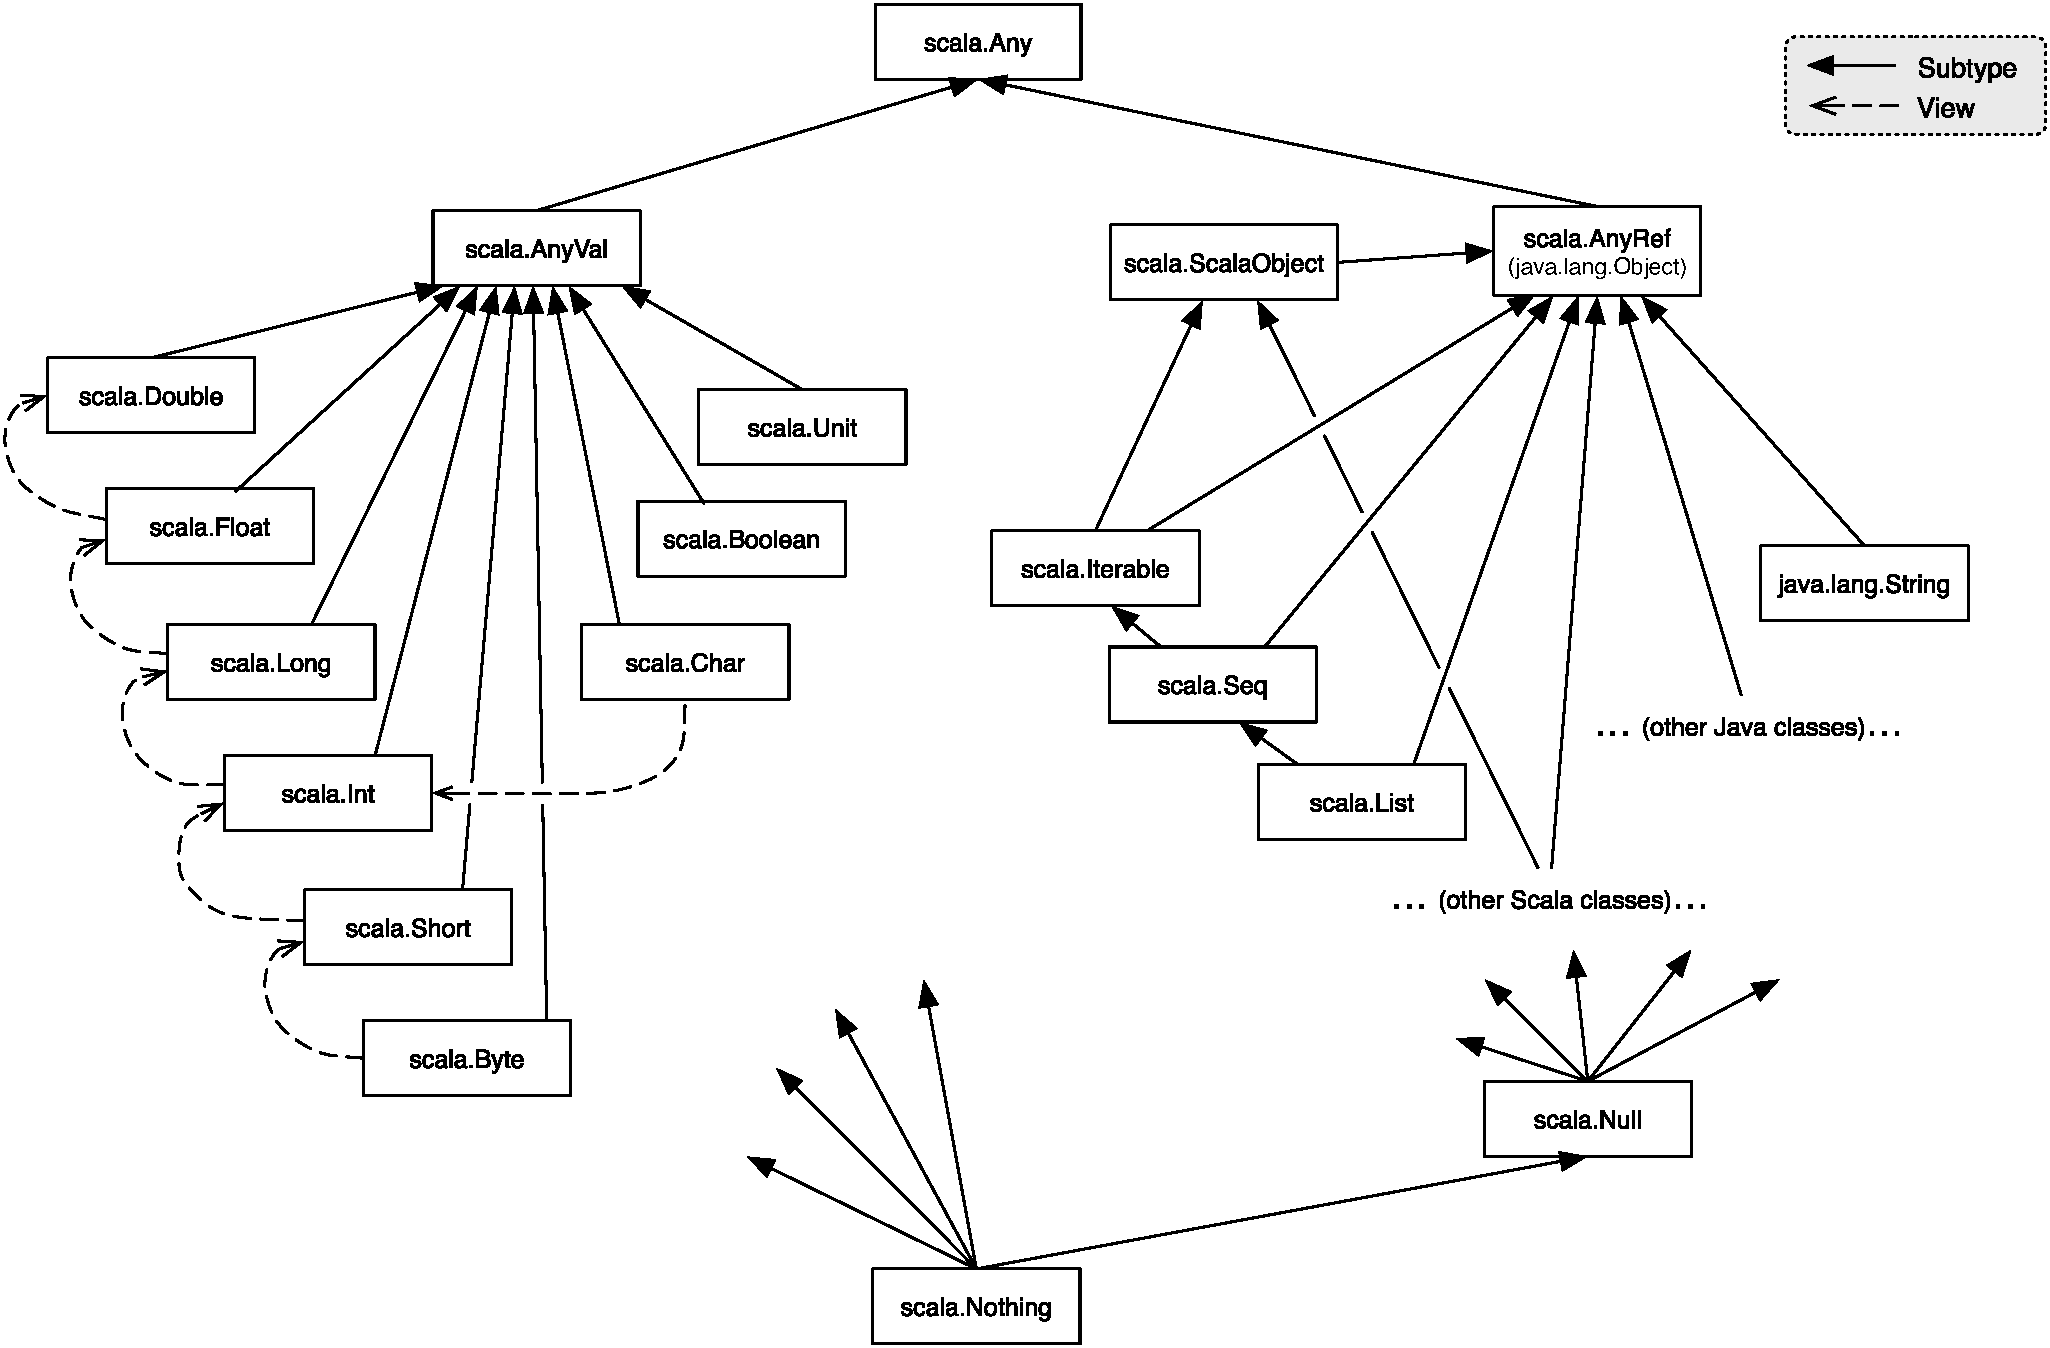
\includegraphics[scale=0.40]{classhierarchy}
\vspace*{-1.5mm}
\caption{Class hierarchy of Scala.}
\end{figure*}

\section{Root Classes}
\label{sec:cls-root}
\label{sec:cls-any}
\label{sec:cls-object}

Figure~\ref{fig:class-hierarchy} illustrates Scala's class
hierarchy.
The root of this hierarchy is formed by class \code{Any}.
Every class in a Scala execution environment inherits directly or
indirectly from this class.  Class \code{Any} has two direct
subclasses: \code{AnyRef} and\code{AnyVal}.

The subclass \code{AnyRef} represents all values which are represented
as objects in the underlying host system. Every user-defined Scala
class inherits directly or indirectly from this class. Furthermore,
every user-defined Scala class also inherits the trait
\code{scala.ScalaObject}.  Classes written in other languages still
inherit from \code{scala.AnyRef}, but not from
\code{scala.ScalaObject}.

The class \code{AnyVal} has a fixed number subclasses, which describe
values which are not implemented as objects in the underlying host
system.

Classes \code{AnyRef} and \code{AnyVal} are required to provide only
the members declared in class \code{Any}, but implementations may add
host-specific methods to these classes (for instance, an
implementation may identify class \code{AnyRef} with its own root
class for objects).

The signatures of these root classes are described by the following
definitions.

\begin{lstlisting}
package scala 
/** The universal root class */
abstract class Any {

  /** Defined equality; abstract here */
  def equals(that: Any): Boolean 

  /** Semantic equality between values of same type */
  final def == (that: Any): Boolean  =  this equals that

  /** Semantic inequality between values of same type */
  final def != (that: Any): Boolean  =  !(this == that)

  /** Hash code; abstract here */
  def hashCode(): Int = $\ldots$

  /** Textual representation; abstract here */
  def toString(): String = $\ldots$

  /** Type test; needs to be inlined to work as given */
  def isInstanceOf[a]: Boolean = this match {
    case x: a => true
    case _ => false
  }

  /** Type cast; needs to be inlined to work as given */ */
  def asInstanceOf[A]: A = this match {
    case x: A => x
    case _ => if (this eq null) this
              else throw new ClassCastException()
  }
}

/** The root class of all value types */
final class AnyVal extends Any 

/** The root class of all reference types */
class AnyRef extends Any {
  def equals(that: Any): Boolean     = this eq that 
  final def eq(that: AnyRef): Boolean   = $\ldots$  // reference equality
  
  def hashCode(): Int = $\ldots$     // hashCode computed from allocation address
  def toString(): String  = $\ldots$ // toString computed from hashCode and class name

/** A mixin class for every user-defined Scala class */
trait ScalaObject extends AnyRef 
\end{lstlisting}

The test ~\lstinline@$x$.asInstanceOf[$T$]@ is treated specially if $T$ is a
numeric value type (\sref{sec:cls-value}. In this case the cast will
be translated to an application of a conversion method ~\lstinline@x.to$T$@ 
(\sref{cls:numeric-value}). For non-numeric values $x$ the operation will raise a
\code{ClassCastException}.

\section{Value Classes}
\label{sec:cls-value}

Value classes are classes whose instances are not represented as
objects by the underlying host system.  All value classes inherit from
class \code{AnyVal}. Scala implementations need to provide the
value classes \code{Unit}, \code{Boolean}, \code{Double}, \code{Float},
\code{Long}, \code{Int}, \code{Char}, \code{Short}, and \code{Byte}
(but are free to provide others as well).
The signatures of these classes are defined in the following.

\subsection{Numeric Value Types} \label{cls:numeric-value}

Classes \code{Double}, \code{Float},
\code{Long}, \code{Int}, \code{Char}, \code{Short}, and \code{Byte}
are together called {\em numeric value types}. Classes \code{Byte},
\code{Short}, or \code{Char} are called {\em subrange types}.
Subrange types, as well as \code{Int} and \code{Long} are called {\em
integer types}, whereas \code{Float} and \code{Double} are called {\em
floating point types}.

Numeric value types are ranked in the following partial order:

\begin{lstlisting}
Byte - Short 
             \
               Int - Long - Float - Double
             / 
        Char 
\end{lstlisting}
\code{Byte} and \code{Short} are the lowest-ranked types in this order, 
whereas \code{Double} is the highest-ranked.  Ranking does {\em not}
imply a conformance (\sref{sec:conformance}) relationship; for
instance \code{Int} is not a subtype of \code{Long}.  However, object
\code{Predef} (\sref{cls:predef}) defines views (\sref{sec:views}) 
from every numeric value type to all higher-ranked numeric value types. Therefore,
lower-ranked types are implicitly converted to higher-ranked types
when required by the context (\sref{sec:impl-conv}).

Given two numeric value types $S$ and $T$, the {\em operation type} of
$S$ and $T$ is defined as follows: If both $S$ and $T$ are subrange
types then the operation type of $S$ and $T$ is \code{Int}.  Otherwise
the operation type of $S$ and $T$ is the larger of the two types wrt
ranking. Given two numeric values $v$ and $w$ the operation type of
$v$ and $w$ is the operation type of their run-time types.

Any numeric value type $T$ supports the following methods.
\begin{itemize}
\item 
Comparison methods for equals (\code{==}), not-equals (\code{!=}),
less-than (\code{<}), greater-than (\code{>}), less-than-or-equals
(\code{<=}), greater-than-or-equals (\code{>=}), which each exist in 7
overloaded alternatives. Each alternative takes a parameter of some
numeric value type. Its result type is type \code{Boolean}. The
operation is evaluated by converting the receiver and its argument to
their operation type and performing the given comparison operation of
that type.
\item
Arithmetic methods addition (\code{+}), subtraction (\code{-}),
multiplication (\code{*}), division (\code{/}), and remainder
(\lstinline@%@), which each exist in 7 overloaded alternatives. Each
alternative takes a parameter of some numeric value type $U$.  Its
result type is the operation type of $T$ and $U$. The operation is
evaluated by converting the receiver and its argument to their
operation type and performing the given arithmetic operation of that
type.
\item
Parameterless arithmethic methods identity (\code{+}) and negation
(\code{-}), with result type $T$.  The first of these returns the
receiver unchanged, whereas the second returns its negation.
\item
Conversion methods \code{toByte}, \code{toShort}, \code{toChar},
\code{toInt}, \code{toLong}, \code{toFloat}, \code{toDouble} which
convert the receiver object to the target type, using the rules of
Java's numeric type cast operation. The conversion might truncate the
numeric value (as when going from \code{Long} to \code{Int} or from
\code{Int} to \code{Byte}) or it might lose precision (as when going
from \code{Double} to \code{Float} or when converting between
\code{Long} and \code{Float}). 
\end{itemize}

Integer numeric value types support in addition the following operations:
\begin{itemize}
\item 
Bit manipulation methods bitewise-and (\code{&}), bitwise-or
{\code{|}}, and bitwise-exclsuive-or (\code{^}), which each exist in 5
overloaded alternatives. Each alternative takes a parameter of some
integer numeric value type. Its result type is the operation type of
$T$ and $U$. The operation is evaluated by converting the receiver and
its argument to their operation type and performing the given bitwise
operation of that type.
\item
A parameterless bit-negation method (\lstinline@~@). Its result type is
the reciver type $T$ or \code{Int}, whichevery is larger.
The operation is evaluated by converting the receiver to the result
type and negating every bit in its value.
\item
Bit-shift methods left-shift (\code{<<}), arithmetic right-shift
(\code{>>}), and unsigned right-shift (\code{>>>}). Each of these
methods of has two overloaded alternatives, which take a parameter $n$
of type \code{Int}, respectively \code{Long}. The result type of the
operation is the reciver type $T$, or \code{Int}, whichever is larger.
The operation is evaluated by converting the receiver to the result
type and performing the specified shift by $n$ bits.
\end{itemize}

Numeric value types also implement operations \code{equals},
\code{hashCode}, and \code{toString} from class \code{Any}.

The \code{equals} method tests whether the argument is a numeric value
type. If this is true, it will perform the \code{==} operation which
is appropriate for that type. That is, the \code{equals} method of a
numeric value type can be thought of being defined as follows:
\begin{lstlisting}
def equals(other: Any): Boolean = other match {
  case that: Byte   => this == that
  case that: Short  => this == that
  case that: Char   => this == that
  case that: Int    => this == that
  case that: Long   => this == that
  case that: Float  => this == that
  case that: Double => this == that
  case _ => false
}
\end{lstlisting}
The \code{hashCode} method returns an integer hashcode that maps equal
numeric values to equal results. It is guaranteed to be the identity for 
for type \code{Int} and for all subrange types.

The \code{toString} method displays its receiver as an integer or
floating point number.

\example As an example, here is the signature of the numeric value type \code{Int}:

\begin{lstlisting}
package scala 
abstract sealed class Int extends AnyVal {
  def == (that: Double): Boolean  // double equality
  def == (that: Float): Boolean   // float equality
  def == (that: Long): Boolean    // long equality
  def == (that: Int): Boolean     // int equality
  def == (that: Short): Boolean   // int equality
  def == (that: Byte): Boolean    // int equality
  def == (that: Char): Boolean    // int equality
  /* analogous for !=, <, >, <=, >= */

  def + (that: Double): Double    // double addition
  def + (that: Float): Double     // float addition
  def + (that: Long): Long        // long addition
  def + (that: Int): Int          // int addition
  def + (that: Short): Int        // int addition
  def + (that: Byte): Int         // int addition
  def + (that: Char): Int         // int addition
  /* analogous for -, *, /, % */
  
  def & (that: Long): Long        // long bitwise and
  def & (that: Int): Int          // int bitwise and
  def & (that: Short): Int        // int bitwise and
  def & (that: Byte): Int         // int bitwise and
  def & (that: Char): Int         // int bitwise and
  /* analogous for |, ^ */

  def << (cnt: Int): Int          // int left shift
  def << (cnt: Long): Int         // long left shift
  /* analogous for >>, >>> */

  def unary_+ : Int               // int identity
  def unary_- : Int               // int negation
  def unary_~ : Int               // int bitwise negation

  def toByte: Byte                // convert to Byte
  def toShort: Short              // convert to Short
  def toChar: Char                // convert to Char
  def toInt: Int                  // convert to Int
  def toLong: Long                // convert to Long
  def toFloat: Float              // convert to Float
  def toDouble: Double            // convert to Double
}
\end{lstlisting}

\subsection{Class \large{\code{Boolean}}}
\label{sec:cls-boolean}

Class \code{Boolean} has only two values: \code{true} and
\code{false}. It implements operations as given in the following
signature:

\begin{lstlisting}
package scala 
abstract sealed class Boolean extends AnyVal {
  def && (p: => Boolean): Boolean  // boolean and
  def || (p: => Boolean): Boolean  // boolean or
  def &  (x: Boolean): Boolean     // boolean strict and
  def |  (x: Boolean): Boolean     // boolean strict or

  def == (x: Boolean): Boolean     // boolean equality
  def != (x: Boolean): Boolean     // boolean inequality

  def unary_!: Boolean             // boolean negation
}
\end{lstlisting}
The class also implements operations \code{equals}, \code{hashCode},
and \code{toString} from class \code{Any}.

The \code{equals} method returns \code{true} if the argument is the
same boolean value as the receiver, \code{false} otherwise.  The
\code{hashCode} method returns \code{1} when invoked on \code{true}, 
and \code{0} when invokend on \code{false}. The \code{toString} method
returns the receiver converted to a string, i.e.\ either \code{"true"}
or \code{"false"}.

\subsection{Class \large{\code{Unit}}}

Class \code{Unit} has only one value: \code{()}. It implements only
the three methods \code{equals}, \code{hashCode}, and \code{toString}
from class \code{Any}.

The \code{equals} method returns \code{true} if the argument is the
unit value \lstinline@()@, \code{false} otherwise.  The
\code{hashCode} method returns a fixed, implementation-specific hash-code, 
The \code{toString} method returns \code{"()"}.

\section{Standard Reference Classes}
\label{cls:reference}

This section presents some standard Scala reference classes which are
treated in a special way in Scala compiler -- either Scala provides
syntactic sugar for them, or the Scala compiler generates special code
for their operations. Other classes in the standard Scala library are
documented in the Scala library documentation by HTML pages.

\subsection{Class \large{\code{String}}}

Scala's \lstinline@String@ class is usually derived from the standard String
class of the underlying host system (and may be identified with
it). For Scala clients the class is taken to support in each case a
method
\begin{lstlisting}
def + (that: Any): String 
\end{lstlisting}
which concatenates its left operand with the textual representation of its
right operand.

\subsection{The \large{\code{Tuple}} classes}

Scala defines tuple classes \lstinline@Tuple$n$@ for $n = 2 \commadots 9$.
These are defined as follows.

\begin{lstlisting}
package scala 
case class Tuple$n$[+a_1, ..., +a_n](_1: a_1, ..., _$n$: a_$n$) {
  def toString = "(" ++ _1 ++ "," ++ $\ldots$ ++ "," ++_$n$ ++ ")"
}
\end{lstlisting}

The implicitly imported \code{Predef} object (\sref{cls:predef}) defines
the names \code{Pair} as an alias of \code{Tuple2} and \code{Triple}
as an alias for \code{Tuple3}.

\subsection{The \large{\code{Function}} Classes}
\label{sec:cls-function}

Scala defines function classes \lstinline@Function$n$@ for $n = 1 \commadots 9$.
These are defined as follows.

\begin{lstlisting}
package scala 
trait Function$n$[-a_1, ..., -a_$n$, +b] {
  def apply(x_1: a_1, ..., x_$n$: a_$n$): b 
  def toString = "<function>" 
}
\end{lstlisting}

\comment{
There is also a module \code{Function}, defined as follows.
\begin{lstlisting}
package scala 
object Function {
  def compose[A](fs: List[A => A]): A => A = {
    x => fs match {
      case Nil => x
      case f :: fs1 => compose(fs1)(f(x))
    }
  }
}
\end{lstlisting}
}
A subclass of \lstinline@Function1@ represents partial functions,
which are undefined on some points in their domain. In addition to the
\code{apply} method of functions, partial functions also have a
\code{isDefined} method, which tells whether the function is defined
at the given argument:
\begin{lstlisting}
class PartialFunction[-A, +B] extends Function1[A, B] {
  def isDefinedAt(x: A): Boolean
}
\end{lstlisting}

The implicitly imported \code{Predef} object (\sref{cls:predef}) defines the name 
\code{Function} as an alias of \code{Function1}.

\subsection{Class \large{\code{Array}}}\label{cls:array}

The class of generic arrays is given as follows.

\begin{lstlisting}
final class Array[A](len: Int) extends Seq[A] {
  def length: Int = len
  def apply(i: Int): A = $\ldots$
  def update(i: Int, x: A): Unit = $\ldots$
  def elements: Iterator[A] = $\ldots$
  def subArray(from: Int, end: Int): Array[A] = $\ldots$
  def filter(p: A => Boolean): Array[A] = $\ldots$
  def map[B](f: A => B): Array[B] = $\ldots$
  def flatMap[B](f: A => Array[B]): Array[B] = $\ldots$
}
\end{lstlisting}
If $T$ is not a type parameter or abstract type, the type Array[$T$]
is represented as the native array type \lstinline{[]$T$} in the
underlying host system. In that case \code{length} returns
the length of the array, \code{apply} means subscribting, and
\code{update} means element update. Because of the syntactic sugar for
\code{apply} and
%\code{update} operations (\sref{sec:impl-conv}, \sref{sec:assignments}),
\code{update} operations (\sref{sec:impl-conv},
we have the following correspondences between Scala and Java/C\# code for
operations on an array \code{xs}:

\begin{lstlisting}
$\mbox{\em Scala}$            $\mbox{\em Java/C\#}$
  xs.length        xs.length
  xs(i)            xs[i]
  xs(i) = e        xs[i] = e
\end{lstlisting}

Arrays also implement the sequence trait \code{scala.Seq}
by defining an \code{elements} method which returns
all elements of the array in an \code{Iterator}.

Because of the tension between parametrized types in Scala and the ad-hoc
implementation of arrays in the host-languages, some subtle points
need to be taken into account when dealing with arrays. These are
explained in the following.

First, unlike arrays in Java or C\#, arrays in Scala are {\em not}
co-variant; That is, $S <: T$ does not imply 
~\lstinline@Array[$S$] $<:$ Array[$T$]@ in Scala.  
However, it is possible to cast an array
of $S$ to an array of $T$ if such a cast is permitted in the host
enironment.

For instance \code{Array[String]} does not conform to
\code{Array[Object]}, even though \code{String} conforms to \code{Object}.
However, it is possible to cast an expression of type
~\lstinline@Array[String]@~ to ~\lstinline@Array[Object]@, and this
cast will succeed withiout raising a \code{ClassCastException}. Example:
\begin{lstlisting}
val xs = new Array[String](2)
// val ys: Array[Object] = xs   // **** error: incompatible types
val ys: Array[Object] = xs.asInstanceOf[Array[Object]] // OK
\end{lstlisting}

Second, for {\em polymorphic arrays}, that have a type parameter or
abstract type $T$ as their element type, a representation different
from
\lstinline@[]T@ might be used. However, it is guaranteed that 
\code{isInstanceOf} and \code{asInstanceOf} still work as if the array 
used the standard representation of monomorphic arrays:
\begin{lstlisting}
val ss = new Array[String](2)

def f[T](xs: Array[T]): Array[String] = 
  if (xs.isInstanceOf[Array[String]]) xs.asInstanceOf[Array[String])
  else throw new Error("not an instance")

f(ss)                                     // returns ss
\end{lstlisting}
The representatuon chosen for polymorphic arrays also guarantees that
polymorphic array creations work as expected. An example is the
following implementation of method \lstinline@mkArray@, which creates
an array of an arbitrary type $T$, given a sequence of $T$'s which
defines its elements.
\begin{lstlisting}
def mkArray[T](elems: Seq[T]): Array[T] = {
  val result = new Array[T](elems.length)
  var i = 0
  for (elem <- elems) {
    result(i) = elem
    i += 1
  }
}
\end{lstlisting}
Note that under Java's erasure model of arrays the method above would
not work as expected -- in fact it would always return an array of
\lstinline@Object@.

Third, in a Java environment there is a method \code{System.arraycopy}
which takes two objects as parameters together with start indices and
a length argument, and copies elements from one object to the other,
provided the objects are arrays of compatible element
types. \code{System.arraycopy} will not work for Scala's polymorphic
arrays because of their different representation. One should instead
use method \code{Array.copy} which is defined in the companion object
of class \lstinline@Array@. This companion object also defines various
constructor methods for arrays, as well as 
the extractor method \code{unapplySeq} (\sref{sec:extractor-patterns})
which enables pattern matching over arrays.
\begin{lstlisting}
package scala
object Array { 
  /** copies array elements from `src' to `dest'. */
  def copy(src: AnyRef, srcPos: Int, 
           dest: AnyRef, destPos: Int, length: Int): Unit = $\ldots$

  /** Concatenate all argument arrays into a single array. */
  def concat[T](xs: Array[T]*): Array[T] = $\ldots$

  /** Create a an array of successive integers. */
  def range(start: Int, end: Int): Array[Int] = $\ldots$

  /** Create an array with given elements. */
  def apply[A <: AnyRef](xs: A*): Array[A] = $\ldots$

  /** Analogous to above. */
  def apply(xs: boolean*): Array[boolean] = $\ldots$
  def apply(xs: byte*)   : Array[byte]    = $\ldots$
  def apply(xs: short*)  : Array[short]   = $\ldots$
  def apply(xs: char*)   : Array[char]    = $\ldots$
  def apply(xs: int*)    : Array[int]     = $\ldots$
  def apply(xs: long*)   : Array[long]    = $\ldots$
  def apply(xs: float*)  : Array[float]   = $\ldots$
  def apply(xs: double*) : Array[double]  = $\ldots$
  def apply(xs: unit*)   : Array[unit]    = $\ldots$

  /** Create an array containing several copies of an element. */
  def make[A](n: Int, elem: A): Array[A] = {

  /** Enables pattern matching over arrays */
  def unapplySeq[A](x: Array[A]): Option[Seq[A]] = Some(x)
}
\end{lstlisting}

\example The following method duplicates a given argument array and returns a pair consisting of the original and the duplicate:
\begin{lstlisting}
def duplicate[T](xs: Array[T]) = {
  val ys = new Array[T](xs.length)
  Array.copy(xs, 0, ys, 0, xs.length)
  (xs, ys)
}
\end{lstlisting}

\section{Class Node}\label{cls:Node}
\begin{lstlisting}
package scala.xml 

trait Node {

  /** the label of this node */
  def label: String               

  /** attribute axis */
  def attribute: Map[String, String] 

  /** child axis (all children of this node) */
  def child: Seq[Node]          

  /** descendant axis (all descendants of this node) */
  def descendant: Seq[Node] = child.toList.flatMap { 
    x => x::x.descendant.asInstanceOf[List[Node]] 
  } 

  /** descendant axis (all descendants of this node) */
  def descendant_or_self: Seq[Node] = this::child.toList.flatMap { 
    x => x::x.descendant.asInstanceOf[List[Node]] 
  } 

  override def equals(x: Any): boolean = x match {
    case that:Node => 
      that.label == this.label && 
        that.attribute.sameElements(this.attribute) && 
          that.child.sameElements(this.child)
    case _ => false
  } 

 /** XPath style projection function. Returns all children of this node
  *  that are labeled with 'that'. The document order is preserved.
  */
    def \(that: Symbol): NodeSeq = {
      new NodeSeq({
        that.name match {
          case "_" => child.toList  
          case _ =>
            var res:List[Node] = Nil 
            for (x <- child.elements if x.label == that.name) {
              res = x::res 
            }
            res.reverse
        }
      }) 
    }

 /** XPath style projection function. Returns all nodes labeled with the 
  *  name 'that' from the 'descendant_or_self' axis. Document order is preserved.
  */
  def \\(that: Symbol): NodeSeq = {
    new NodeSeq(
      that.name match {
        case "_" => this.descendant_or_self 
        case _ => this.descendant_or_self.asInstanceOf[List[Node]].
        filter(x => x.label == that.name) 
      })
  }

  /** hashcode for this XML node */
  override def hashCode() = 
    Utility.hashCode(label, attribute.toList.hashCode(), child) 

  /** string representation of this node */
  override def toString() = Utility.toXML(this) 

}
\end{lstlisting}

\newpage
\section{The \large{\code{Predef}} Object}\label{cls:predef}

The \code{Predef} object defines standard functions and type aliases
for Scala programs. It is always implicitly imported, so that all its
defined members are available without qualification. Its definition
for the JVM environment conforms to the following signature:

\begin{lstlisting}
package scala
object Predef {

  // classOf ---------------------------------------------------------

  /** Return the runtime representation of a class type. */
  def classOf[T]: Class = null  // this is a dummy, classOf is handled by compiler.

  // Standard type aliases ---------------------------------------------

  type byte    = scala.Byte
  type short   = scala.Short
  type char    = scala.Char
  type int     = scala.Int
  type long    = scala.Long
  type float   = scala.Float
  type double  = scala.Double
  type boolean = scala.Boolean
  type unit    = scala.Unit

  type String = java.lang.String
  type NullPointerException = java.lang.NullPointerException
  type Throwable = java.lang.Throwable
  type Function[-a,+b] = Function1[a,b]

  // Aliasses and extractors for tuples ------------------------

  type Pair[+A, +B] = Tuple2[A, B]
  object Pair {
    def apply[A, B](x: A, y: B) = Tuple2(x, y)
    def unapply[A, B](x: Tuple2[A, B]): Option[Tuple2[A, B]] = Some(x)
  }

  type Triple[+A, +B, +C] = Tuple3[A, B, C]
  object Triple {
    def apply[A, B, C](x: A, y: B, z: C) = Tuple3(x, y, z)
    def unapply[A, B, C](x: Tuple3[A, B, C]): Option[Tuple3[A, B, C]] = Some(x)
  }
\end{lstlisting}
\newpage
\begin{lstlisting}
  // The ``catch-all'' view ----------------------------------------

  implicit def identity[A](x: A): A = x

  // Views into class Ordered

  implicit def int2ordered(x: Int): Ordered[Int] = new Ordered[Int] with Proxy {
    def self: Any = x
    def compare[B >: Int <% Ordered[B]](y: B): Int = y match {
      case y1: Int =>
        if (x < y1) -1
        else if (x > y1) 1
        else 0
      case _ => -(y compare x)
    }
  }

  // The implementations of following methods are analogous to the last one:

  implicit def char2ordered(x: Char): Ordered[Char] = $\ldots$ 
  implicit def long2ordered(x: Long): Ordered[Long] = $\ldots$ 
  implicit def float2ordered(x: Float): Ordered[Float] = $\ldots$
  implicit def double2ordered(x: Double): Ordered[Double] = $\ldots$
  implicit def boolean2ordered(x: Boolean): Ordered[Boolean] = $\ldots$

  implicit def seq2ordered[A <% Ordered[A]](xs: Array[A]): Ordered[Seq[A]] = 
    new Ordered[Seq[A]] with Proxy {
      def compare[B >: Seq[A] <% Ordered[B]](that: B): Int = that match {
        case that: Seq[A] =>
          var res = 0
          val these = this.elements
          val those = that.elements
          while (res == 0 && these.hasNext)
            res = if (!those.hasNext) 1 else these.next compare those.next
        case _ => - (that compare xs)
    }

  implicit def string2ordered(x: String): Ordered[String] = 
    new Ordered[String] with Proxy {
      def self: Any = x
      def compare [b >: String <% Ordered[b]](y: b): int = y match {
        case y1: String => x compare y1
        case _ => -(y compare x)
      }
    }
\end{lstlisting}
\newpage
\begin{lstlisting}
  implicit def tuple2ordered[a1 <% Ordered[a1], a2 <% Ordered[a2]]
                            (x: Tuple2[a1, a2]): Ordered[Tuple2[a1, a2]] = 
    new Ordered[Tuple2[a1, a2]] with Proxy {
      def self: Any = x
      def compare[T >: Tuple2[a1, a2] <% Ordered[T]](y: T): Int = y match {
        case y: Tuple2[a1, a2] => 
          val res = x._1 compare y._1
          if (res == 0) x._2 compare y._2
          else res
        case _ => -(y compare x)
      }
    }

  // Analogous for Tuple3 to Tuple9

  // Views into class Seq

  implicit def string2seq(str: String): Seq[Char] = new Seq[Char] {
    def length = str.length()
    def elements = Iterator.fromString(str)
    def apply(n: Int) = str.charAt(n)
    override def hashCode(): Int = str.hashCode()
    override def equals(y: Any): Boolean = (str == y)
    override protected def stringPrefix: String = "String"
  }

  // Views from primitive types to Java's boxed types

  implicit def byte2Byte(x: Byte) = new java.lang.Byte(x)
  implicit def short2Short(x: Short) = new java.lang.Short(x)
  implicit def char2Character(x: Char) = new java.lang.Character(x)
  implicit def int2Integer(x: Int) = new java.lang.Integer(x)
  implicit def long2Long(x: Long) = new java.lang.Long(x)
  implicit def float2Float(x: Float) = new java.lang.Float(x)
  implicit def double2Double(x: Double) = new java.lang.Double(x)
  implicit def boolean2Boolean(x: Boolean) = new java.lang.Boolean(x)

  // Numeric conversion views

  implicit def byte2short(x: Byte): Short = x.toShort
  implicit def byte2int(x: Byte): Int = x.toInt
  implicit def byte2long(x: Byte): Long = x.toLong
  implicit def byte2float(x: Byte): Float = x.toFloat
  implicit def byte2double(x: Byte): Double = x.toDouble

\end{lstlisting}
\newpage
\begin{lstlisting}
  implicit def short2int(x: Short): Int = x.toInt
  implicit def short2long(x: Short): Long = x.toLong
  implicit def short2float(x: Short): Float = x.toFloat
  implicit def short2double(x: Short): Double = x.toDouble

  implicit def char2int(x: Char): Int = x.toInt
  implicit def char2long(x: Char): Long = x.toLong
  implicit def char2float(x: Char): Float = x.toFloat
  implicit def char2double(x: Char): Double = x.toDouble

  implicit def int2long(x: Int): Long = x.toLong
  implicit def int2float(x: Int): Float = x.toFloat
  implicit def int2double(x: Int): Double = x.toDouble

  implicit def long2float(x: long): Float = x.toFloat
  implicit def long2double(x: long): Double = x.toDouble

  implicit def float2double(x: Float): Double = x.toDouble

// Errors and asserts -----------------------------------------

  def error(message: String): Nothing = throw new Error(message)

  def exit(): Nothing = exit(0)
  def exit(status: Int): Nothing = {
    java.lang.System.exit(status)
    throw new Throwable()
  }

  def assert(assertion: Boolean): Unit =
    if (!assertion)
      throw new Error("assertion failed")

  def assert(assertion: Boolean, message: Any): Unit =
    if (!assertion)
      throw new Error("assertion failed: " + message)

  def assume(assumption: Boolean): Unit =
    if (!assumption)
      throw new Error("assumption failed")

  def assume(assumption: Boolean, message: Any): Unit =
    if (!assumption)
      throw new Error("assumption failed: " + message)
}
\end{lstlisting}

\comment{
\subsection{Base Classes}
\label{sec:base-classes}

For every template, class type and constructor invocation we define
two sets of class types: the {\em base classes} and {\em mixin base
classes}. Their definitions are as follows.

The {\em mixin base classes} of a template 
~\lstinline@$sc$ with $mt_1$ with $\ldots$ with $mt_n$ {$\stats\,$}@~ 
are 
the reduced union (\sref{sec:base-classes-member-defs}) of the base classes of all
mixins $mt_i$. The mixin base classes of a class type $C$ are the
mixin base classes of the template augmented by $C$ itself. The
mixin base classes of a constructor invocation of type $T$ are the
mixin base classes of class $T$.

The {\em base classes} of a template consist are the reduced union of
the base classes of its superclass and the template's mixin base
classes.  The base classes of class \lstinline@scala.Any@ consist of
just the class itself. The base classes of some other class type $C$
are the base classes of the template represented by $C$ augmented by
$C$ itself.  The base classes of a constructor invocation of type $T$
are the base classes of $T$.

The notions of mixin base classes and base classes are extended from
classes to arbitrary types following the definitions of
\sref{sec:base-classes-member-defs}.

\comment{
If two types in the base class sequence of a template refer to the
same class definition, then that definition must define a trait
(\sref{sec:traits}), and the type that comes later in the sequence must
conform to the type that comes first. 
(\sref{sec:base-classes-member-defs}).
}

\example 
Consider the following class definitions:
\begin{lstlisting}
class A 
class B extends A 
trait C extends A 
class D extends A 
class E extends B with C with D 
class F extends B with D with E 
\end{lstlisting} 
The mixin base classes and base classes of classes \code{A-F} are given in
the following table:
\begin{quote}\begin{tabular}{|l|l|l|} \hline
 \ & Mixin base classes & Base classes \\  \hline
A & A & A, ScalaObject, AnyRef, Any \\
B & B & B, A, ScalaObject, AnyRef, Any \\
C & C & C, A, ScalaObject, AnyRef, Any \\
D & D & D, A, ScalaObject, AnyRef, Any \\
E & C, D, E & E, B, C, D, A, ScalaObject, AnyRef, Any \\
F & C, D, E, F & F, B, D, E, C, A, ScalaObject, AnyRef, Any \\ \hline
\end{tabular}\end{quote}
Note that \code{D} is inherited twice by \code{F}, once directly, the
other time indirectly through \code{E}. This is permitted, since
\code{D} is a trait.
}


\bibliographystyle{alpha}
\bibliography{Scala}
\appendix
% $Id$

\chapter{Scala Syntax Summary}\label{sec:syntax}
\todo{introduce SeqPattern syntax}

The lexical syntax of Scala is given by the following grammar in EBNF
form.

{\small
\begin{lstlisting}
  upper            ::=  `A' | $\ldots$ | `Z' | `$\Dollar$' | `_' $\mbox{\rm\em and Unicode Lu}$
  lower            ::=  `a' | $\ldots$ | `z' $\mbox{\rm\em and Unicode Ll}$
  letter           ::=  upper | lower $\mbox{\rm\em and Unicode categories Lo, Lt, Nl}$
  digit            ::=  `0' | $\ldots$ | `9'
  opchar           ::=  $\mbox{\rm\em ``all other characters in
  \U{0020-007F} and Unicode categories}$
                        $\mbox{\rm\em  Sm, So except parentheses ([{}]) and periods''}$

  op               ::=  opchar {opchar} 
  varid            ::=  lower idrest
  plainid          ::=  upper idrest
                     |  varid
                     |  op
  id               ::=  plainid
                     |  `\`' stringLit `\`'
  idrest           ::=  {letter | digit} [`_' op]

  integerLiteral   ::=  (decimalNumeral | hexNumeral | octalNumeral) ['L' | 'l']
  decimalNumeral   ::=  `0' | nonZeroDigit {digit}
  hexNumeral       ::=  `0' `x' hexDigit {hexDigit}
  octalNumeral     ::=  `0' octalDigit {octalDigit}
  digit            ::=  `0' | nonZeroDigit
  nonZeroDigit     ::=  `1' | $\ldots$ | `9'
  octalDigit       ::=  `0' | $\ldots$ | `7'

  floatingPointLiteral 
                   ::=  digit {digit} `.' {digit} [exponentPart] [floatType]
                     |  `.' digit {digit} [exponentPart] [floatType]
                     |  digit {digit} exponentPart [floatType]
                     |  digit {digit} [exponentPart] floatType
  exponentPart     ::=  ('E' | 'e') ['+' | '-'] digit {digit}
  floatType        ::=  'F' | 'f' | 'D' | 'd'

  booleanLiteral   ::=  true | false

  characterLiteral ::= `\'' printableChar `\''
                     |  `\'' charEscapeSeq `\''

  stringLiteral    ::=  `"' {stringElement} `"'
                     |  `"""' multiLineChars `"""'
  stringElement    ::=  printableCharNoDoubleQuote 
                     |  charEscapeSeq
  multiLineChars   ::=  {['"'] ['"'] charNoDoubleQuote}

  symbolLiteral    ::=  `'' plainid

  comment          ::=  `/*' $\mbox{\rm\em ``any sequence of characters''}$ `*/'
                     |  `//' $\mbox{\rm\em ``any sequence of characters up to end of line''}$

  nl               ::=  $\mbox{\rm\em ``new line character''}$
  semi             ::=  `;' |  nl {nl}       
\end{lstlisting}}

The context-free syntax of Scala is given by the following EBNF
grammar.

{\small
\begin{lstlisting}
  Literal           ::=  integerLiteral
                      |  floatingPointLiteral
                      |  booleanLiteral
                      |  characterLiteral
                      |  stringLiteral
                      |  symbolLiteral
                      |  null

  QualId            ::=  id {`.' id}
  ids               ::=  id {`,' id}

  Path              ::=  StableId
                      |  [id `.'] this
  StableId          ::=  id
                      |  Path `.' id
                      |  [id '.'] super [ClassQualifier] `.' id
  ClassQualifier    ::=  `[' id `]'

  Type              ::=  InfixType `=>' Type
                      |  `(' [`=>' Type] `)' `=>' Type
                      |  InfixType [ExistentialClause]
  ExistentialClause ::=  forSome `{' ExistentialDcl {semi ExistentialDcl}} `}'
  ExistentialDcl    ::=  type TypeDcl 
                      |  val ValDcl
  InfixType         ::=  CompoundType {id [nl] CompoundType}
  CompoundType      ::=  AnnotType {with AnnotType} [Refinement]
                      |  Refinement
  AnnotType         ::=  {Annotation} SimpleType
  SimpleType        ::=  SimpleType TypeArgs
                      |  SimpleType `#' id
                      |  StableId
                      |  Path `.' type
                      |  `(' Types [`,'] ')'
  TypeArgs          ::=  `[' Types `]'
  Types             ::=  Type {`,' Type}
  Refinement        ::=  [nl] `{' RefineStat {semi RefineStat} `}'
  RefineStat        ::=  Dcl
                      |  type TypeDef
                      |
  TypePat           ::=  Type

  Ascription        ::=  `:' CompoundType
                      |  `:' Annotation {Annotation} 
                      |  `:' `_' `*'

  Expr              ::=  (Bindings | id) `=>' Expr
                      |  Expr1
  Expr1             ::=  if `(' Expr `)' {nl} Expr [[semi] else Expr]
                      |  while `(' Expr `)' {nl} Expr
                      |  try `{' Block `}' [catch  `{' CaseClauses `}'] 
                         [finally Expr]
                      |  do Expr [semi] while `(' Expr ')'
                      |  for (`(' Enumerators `)' | `{' Enumerators `}') 
                         {nl} [yield] Expr
                      |  throw Expr
                      |  return [Expr]
                      |  [SimpleExpr `.'] id `=' Expr
                      |  SimpleExpr1 ArgumentExprs `=' Expr
                      |  PostfixExpr
                      |  PostfixExpr Ascription
                      |  PostfixExpr match `{' CaseClauses `}'
  PostfixExpr       ::=  InfixExpr [id [nl]]
  InfixExpr         ::=  PrefixExpr
                      |  InfixExpr id [nl] InfixExpr
  PrefixExpr        ::=  [`-' | `+' | `~' | `!'] SimpleExpr 
  SimpleExpr        ::=  new (ClassTemplate | TemplateBody)
                      |  BlockExpr
                      |  SimpleExpr1 [`_']
  SimpleExpr1       ::=  Literal
                      |  Path
                      |  `_'
                      |  `(' [Exprs [`,']] `)'
                      |  SimpleExpr `.' id 
                      |  SimpleExpr TypeArgs
                      |  SimpleExpr1 ArgumentExprs
                      |  XmlExpr
  Exprs             ::=  Expr {`,' Expr}
  ArgumentExprs     ::=  `(' [Exprs [`,']] ')'
                      |  [nl] BlockExpr
  BlockExpr         ::=  `{' CaseClauses `}'
                      |  `{' Block `}'
  Block             ::=  {BlockStat semi} [ResultExpr]
  BlockStat         ::=  Import
                      |  [implicit] Def
                      |  {LocalModifier} TmplDef
                      |  Expr1
                      |
  ResultExpr        ::=  Expr1
                      |  (Bindings | id `:' CompoundType) `=>' Block

  Enumerators       ::=  Generator {semi Enumerator}
  Enumerator        ::=  Generator
                      |  Guard
                      |  val Pattern1 `=' Expr
  Generator         ::=  Pattern1 `<-' Expr [Guard]

  CaseClauses       ::=  CaseClause { CaseClause }
  CaseClause        ::=  case Pattern [Guard] `=>' Block 
  Guard             ::=  `if' PostfixExpr

  Pattern           ::=  Pattern1 { `|' Pattern1 }
  Pattern1          ::=  varid `:' TypePat
                      |  `_' `:' TypePat
                      |  Pattern2
  Pattern2          ::=  varid [`@' Pattern3]
                      |  Pattern3
  Pattern3          ::=  SimplePattern
                      |  SimplePattern { id [nl] SimplePattern }
  SimplePattern     ::=  `_'
                      |  varid
                      |  Literal
                      |  StableId
                      |  StableId `(' [Patterns [`,']] `)'
                      |  StableId `(' [Patterns `,'] `_' `*' `)'
                      |  `(' [Patterns [`,']] `)'
                      |  XmlPattern
  Patterns          ::=  Pattern [`,' Patterns]
                      |  `_' *

  TypeParamClause   ::=  `[' VariantTypeParam {`,' VariantTypeParam} `]'
  FunTypeParamClause::=  `[' TypeParam {`,' TypeParam} `]'
  VariantTypeParam  ::=  [`+' | `-'] TypeParam
  TypeParam         ::=  id [>: Type] [<: Type] [<% Type]
  ParamClauses      ::=  {ParamClause} [[nl] `(' implicit Params `)']
  ParamClause       ::=  [nl] `(' [Params] ')'} 
  Params            ::=  Param {`,' Param}
  Param             ::=  {Annotation} id [`:' ParamType]
  ParamType         ::=  Type 
                      |  `=>' Type 
                      |  Type `*'
  ClassParamClauses ::=  {ClassParamClause} 
                         [[nl] `(' implicit ClassParams `)']
  ClassParamClause  ::=  [nl] `(' [ClassParams] ')'
  ClassParams       ::=  ClassParam {`' ClassParam}
  ClassParam        ::=  {Annotation} [{Modifier} (`val' | `var')] 
                         id [`:' ParamType]
  Bindings          ::=  `(' Binding {`,' Binding `)'
  Binding           ::=  id [`:' Type]

  Modifier          ::=  LocalModifier 
                      |  AccessModifier
                      |  override
  LocalModifier     ::=  abstract
                      |  final
                      |  sealed
                      |  implicit
                      |  lazy
  AccessModifier    ::=  (private | protected) [AccessQualifier]
  AccessQualifier   ::=  `[' (id | this) `]'

  Annotation        ::=  `@' AnnotationExpr [nl]
  AnnotationExpr    ::=  Constr [[nl] `{' {NameValuePair} `}']
  NameValuePair     ::=  val id `=' PrefixExpr

  TemplateBody      ::=  [nl] `{' [SelfType] TemplateStat {semi TemplateStat} `}'
  TemplateStat      ::=  Import
                      |  {Annotation} {Modifier} Def
                      |  {Annotation} {Modifier} Dcl
                      |  Expr
                      |
  SelfType          ::=  id [`:' Type] `=>'
                      |  this `:' Type `=>' 

  Import            ::=  import ImportExpr {`,' ImportExpr}
  ImportExpr        ::=  StableId `.' (id | `_' | ImportSelectors)
  ImportSelectors   ::=  `{' {ImportSelector `,'} (ImportSelector | `_') `}'
  ImportSelector    ::=  id [`=>' id | `=>' `_']

  Dcl               ::=  val ValDcl
                      |  var VarDcl
                      |  def FunDcl
                      |  type {nl} TypeDcl

  ValDcl            ::=  ids `:' Type
  VarDcl            ::=  ids `:' Type
  FunDcl            ::=  FunSig [`:' Type]
  FunSig            ::=  id [FunTypeParamClause] ParamClauses
  TypeDcl           ::=  id [TypeParamClause] [`>:' Type] [`<:' Type]

  Def               ::=  val PatDef
                      |  var VarDef
                      |  def FunDef
                      |  type {nl} TypeDef
                      |  TmplDef
  PatDef            ::=  Pattern2 {`,' Pattern2} [`:' Type] `=' Expr
  VarDef            ::=  PatDef
                      |  ids `:' Type `=' `_'
  FunDef            ::=  FunSig `:' Type `=' Expr
                      |  FunSig [nl] `{' Block `}'
                      |  this ParamClause ParamClauses 
                         (`=' ConstrExpr | [nl] ConstrBlock)
  TypeDef           ::=  id [TypeParamClause] `=' Type

  TmplDef           ::=  [case] class ClassDef
                      |  [case] object ObjectDef
                      |  trait TraitDef
  ClassDef          ::=  id [TypeParamClause] {Annotation} [AccessModifier] 
                         ClassParamClauses ClassTemplateOpt 
  TraitDef          ::=  id [TypeParamClause] TraitTemplateOpt
  ObjectDef         ::=  id ClassTemplateOpt
  ClassTemplateOpt  ::=  extends ClassTemplate | [[extends] TemplateBody]
  TraitTemplateOpt  ::=  extends TraitTemplate | [[extends] TemplateBody]
  ClassTemplate     ::=  [EarlyDefs] ClassParents [TemplateBody]
  TraitTemplate     ::=  [EarlyDefs] TraitParents [TemplateBody]
  ClassParents      ::=  Constr {with AnnotType}
  TraitParents      ::=  AnnotType {with AnnotType}
  Constr            ::=  AnnotType {ArgumentExprs}
  EarlyDefs         ::= `{' [EarlyDef {semi EarlyDef}] `}' with
  EarlyDef          ::=  Annotations Modifiers PatDef  

  ConstrExpr        ::=  SelfInvocation 
                      |  ConstrBlock
  ConstrBlock       ::=  `{' SelfInvocation {semi BlockStat} `}'
  SelfInvocation    ::=  this ArgumentExprs {ArgumentExprs}

  TopStatSeq        ::=  TopStat {semi TopStat}
  TopStat           ::=  {Annotation} {Modifier} TmplDef
                      |  Import
                      |  Packaging
                      |
  Packaging         ::=  package QualId [nl] `{' TopStatSeq `}'

  CompilationUnit   ::=  [package QualId semi] TopStatSeq
\end{lstlisting}
}

\todo{Add 
SimplePattern    ::= StableId  [TypePatArgs] [`(' [SeqPatterns [`,']] `)']
TypePatArgs ::= `[' TypePatArg {`,' TypePatArg} `]'
TypePatArg    ::=  `_' |   varid}

% $Id$

\chapter{Change Log}

\section*{Changes in Version 2.5.0}

\subsection*{Early object initialization}

It is now possible to initialize some fields of an object before any
parent constructors are called (\sref{sec:early-defs}). This is particularly useful for
traits, which do not have normal constructor parameters. Example:
\begin{lstlisting}
trait Greeting {
  val name: String
  val msg = "How are you, "+name
}
class C extends {
  val name = "Bob"
} with Greeting {
  println(msg)
}
\end{lstlisting}
In the code above, the field \code{name} is initialized before the
constructor of \code{Greeting} is called. Therefore, field \lstinline@msg@ in
class \code{Greeting} is properly initialized to \code{"How are you, Bob"}.

\subsection*{For-comprehensions, revised}

The syntax of for-comprehensions has been changed (\sref{sec:for-comprehensions}). For example:

\begin{lstlisting}
for (val x <- List(1, 2, 3); x % 2 == 0) println(x)
\end{lstlisting}

is now written

\begin{lstlisting}
for (x <- List(1, 2, 3) if x % 2 == 0) println(x)
\end{lstlisting}

The old syntax is still available but will be deprecated in the
future. 

\subsection*{Implicit anonymous functions}

It is now possible to define anonymous functions 
using underscores in parameter position (\sref{sec:impl-anon-fun}).
For instance, 
the expressions in the left column are each function values which 
expand to the anonymous functions on their right.
\begin{lstlisting}
_ + 1                  x => x + 1
_ * _                  (x1, x2) => x1 + x2
(_: int) * 2           (x: int) => (x: int) * 2
if (_) x else y        x => if (x) x else y
_.map(f)               x => x.map(f)
_.map(_ + 1)           x => x.map(y => y + 1)
\end{lstlisting}
As a special case (\sref{sec:meth-vals}), a partially unapplied method is now designated
~\lstinline@m _@~~ instead of the previous notation ~\lstinline@&m@.

The new notation will displace the special syntax forms
\lstinline@.m()@ for abstracting over method receivers and
\lstinline@&m@ for treating an unapplied method as a function value.
For the time being, the old syntax forms are still available, 
but they will be deprecated in the future.

\subsection*{Pattern matching anonymous functions, refined}

It is now possible to use case clauses to define a function value
directly for functions of arities greater than one
(\sref{sec:pattern-closures}).  Previously, only unary functions could
be defined that way. Example:
\begin{lstlisting}
def scalarProduct(xs: Array[Double], ys: Array[Double]) = 
  (0.0 /: (xs zip ys)) {
    case (a, (b, c)) => a + b * c
  }
\end{lstlisting}

\section*{Changes in Version 2.4.0}

\subsection*{Object-local private and protected}

The \lstinline@private@ and \lstinline@protected@ modifiers now accept
a \lstinline@[this]@ qualifier (\sref{sec:modifiers}). A definition $M$ which is labelled
\lstinline@private[this]@ is private, and in addition can be accessed
only from within the current object. That is, the only legal prefixes
for $M$ are \lstinline@this@ or \lstinline@$C$.this@.  Analogously, a
definition $M$ which is labelled \lstinline@protected[this]@ is
protected, and in addition can be accessed only from within the
current object.

\subsection*{Tuples, revised}

The syntax for tuples has been changed from $\{\ldots\}$ to $(\ldots)$ (\sref{sec:tuples}). For any
sequence of types $T_1 \commadots T_n$,

\begin{tabular}{lll}
$(T_1 \commadots T_n)$ &is a shorthand for&
\lstinline@Tuple$n$[$T_1 \commadots T_n$]@.  
\end{tabular}

Analogously, for any sequence of expressions or patterns $x_1
\commadots x_n$,

\begin{tabular}{lll}
$(x_1 \commadots x_n)$ &is a shorthand for&
\lstinline@Tuple$n$($x_1 \commadots x_n$)@.
\end{tabular}

\subsection*{Access modifiers for primary constructors}

The primary constructor of a class can now be marked \code{private} or
\code{protected} (\sref{sec:class-defs}). If such an access modifier is given, it comes
between the name of the class and its value parameters. Example:
\begin{lstlisting}
class C[T] private (x: T) { ... }
\end{lstlisting}

\subsection*{Annotations}

The support for attributes has been extended and its syntax changed
(\sref{sec:annotations}).  Attributes are now called {\em
  annotations}. The syntax has been changed to follow Java's
conventions, e.g. \lstinline^@attribute^ instead of
\lstinline@[attribute]@. The old syntax is still available but will be
deprecated in the future.

Annotations are now serialized so that they can be read by
compile-time or run-time tools. Class \code{scala.Annotation} has two
sub-traits which are used to indicate how annotations are
retained. Instances of an annotation class inheriting from trait
\code{scala.ClassfileAnnotation} will be stored in the generated class
files. Instances of an annotation class inheriting from trait
\code{scala.StaticAnnotation} will be visible to the Scala type-checker
in every compilation unit where the annotated symbol is accessed. 

\subsection*{Decidable subtyping}

The implementation of subtyping has been changed to prevent infinite
recursions. Termination of subtyping is now ensured by a new
restriction of class graphs to be finitary
(\sref{sec:inheritance-closure}).

\subsection*{Case classes cannot be abstract}

It is now explicitly ruled out that case classes can be abstract
(\sref{sec:modifiers}). The specification was silent on this point
before, but did not explain how abstract case classes were
treated. The Scala compiler allowed the idiom.

\subsection*{New syntax for self aliases and self types}

It is now possible to give an explicit alias name and/or type for the
self reference \code{this} (\sref{sec:templates}). For instance, in
\begin{lstlisting}
class C { self: D => 
  ...
}
\end{lstlisting}
the name \code{self} is introduced as an alias for \code{this} within
\code{C} and the self type (\sref{sec:class-defs}) of \code{C} is
assumed to be \code{D}. This construct is introduced now in order to
replace eventually both the qualified this construct \code{C.this} and
the \code{requires} clause in Scala.

\subsection*{Assignment Operators}

It is now possible to combine operators with assignments (\sref{sec:assops}). Example:
\begin{lstlisting}
var x: int = 0
x += 1
\end{lstlisting}

\section*{Changes in Version 2.3.2 (23-Jan-2007)}

\subsection*{Extractors}

It is now possible to define patterns independently of case classes,
using \code{unapply} methods in extractor objects
(\sref{sec:extractor-patterns}). 
Here is an example:
\begin{lstlisting}
object Twice {                              
  def apply(x:Int): int = x*2
  def unapply(z:Int): Option[int] = if (z%2==0) Some(z/2) else None
}
val x = Twice(21) 
x match { case Twice(n) => Console.println(n) } // prints 21
\end{lstlisting}
In the example, \lstinline@Twice@ is an extractor object with two methods:
\begin{itemize}
\item
The \code{apply} method is used to build even numbers.
\item
The \code{unapply} method is used to decompose an even number; it is
in a sense the reverse of \code{apply}. \lstinline@unapply@ methods return option types: 
\code{Some(...)} for a match that suceeds, \code{None} for a match that fails.
Pattern variables are returned as the elements of \code{Some}. If there are several
variables, they are grouped in a tuple.
\end{itemize}
In the second-to-last line, \code{Twice}'s \code{apply} method is used
to construct a number \code{x}. In the last line, \code{x} is tested
against the pattern
\code{Twice(n)}. This pattern succeeds for even numbers and assigns to the variable
\code{n} one half of the number that was tested. The pattern match makes use of
the \code{unapply} method of object \code{Twice}. More details on extractors can be found
in the paper ``Matching Objects with Patterns'' by Emir, Odersky and Williams.
 
\subsection*{Tuples}

A new lightweight syntax for tuples has been introduced
(\sref{sec:tuples}). For any sequence of types $T_1 \commadots T_n$,

\begin{tabular}{lll}
$\{T_1 \commadots T_n \}$ &is a shorthand for&
\lstinline@Tuple$n$[$T_1 \commadots T_n$]@.  
\end{tabular}

Analogously, for any sequence of expressions or patterns $x_1
\commadots x_n$,

\begin{tabular}{lll}
$\{x_1 \commadots x_n \}$ &is a shorthand for&
\lstinline@Tuple$n$($x_1 \commadots x_n$)@.
\end{tabular}

\subsection*{Infix operators of greater arities}

It is now possible to use methods which have more than one parameter
as infix operators (\sref{sec:infix-operations}). In this case, all
method arguments are written as a normal parameter list in parentheses. Example:
\begin{lstlisting}
class C {
  def +(x: int, y: String) = ...
}
val c = new C
c + (1, "abc")
\end{lstlisting}

\subsection*{Deprecated attribute}

A new standard attribute \lstinline@deprecated@ is available (\sref{sec:annotations}). If a
member definition is marked with this attribute, any reference to the
member will cause a ``deprecated'' warning message to be emitted.

\section*{Changes in Version 2.3.0 (23-Nov-2006)}

\subsection*{Procedures} A simplified syntax for functions returning
\lstinline@unit@ has been introduced (\sref{sec:procedures}). 
Scala now allows the following shorthands:

\begin{tabbing}
\lstinline@def f(params)@     \tab\tab\tab \=$\mbox{for}$  \tab
\lstinline@def f(params): unit@ \\
\lstinline@def f(params) { ... }@  \>$\mbox{for}$    \tab
\lstinline@def f(params): unit = { ... }@
\end{tabbing}

\subsection*{Type Patterns} The syntax of types in patterns has been 
refined (\sref{sec:type-patterns}). Scala now distinguishes between
type variables (starting with a lower case letter) and types as type
arguments in patterns.  Type variables are bound in the pattern. Other
type arguments are, as in previous versions, erased. The Scala
compiler will now issue an ``unchecked'' warning at places where type
erasure might compromise type-safety.

\subsection*{Standard Types} 

The recommended names for the two bottom classes in Scala's type
hierarchy have changed as follows:
\begin{lstlisting}
All      ==>     Nothing
AllRef   ==>     Null
\end{lstlisting}
The old names are still available as type aliases.

\section*{Changes in Version 2.1.8 (23-Aug-2006)}

\subsection*{Visibility Qualifier for protected}

Protected members can now have a visibility qualifier (\sref{sec:modifiers}),
e.g. \lstinline@protected[<qualifier>]@. In particular, one can now
simulate package protected access as in Java writing
\begin{lstlisting}
  protected[P] def X ...
\end{lstlisting}
where \code{P} would name the package containing \code{X}.

\subsection*{Relaxation of Private Acess}

Private members of a class can now be referenced from the companion
module of the class and vice versa (\sref{sec:modifiers})

\subsection*{Implicit Lookup}

The lookup method for implicit definitions has been generalized
(\sref{sec:impl-params}). 
When searching for an implicit definition matching a type $T$, now are
considered
\begin{enumerate}
\item all identifiers accessible without prefix, and
\item all members of companion modules of classes associated with $T$.
\end{enumerate}
(The second clause is more general than before). 
Here, a class is {\em associated} with a type $T$ if it is referenced
by some part of $T$, 
or if it is a base class of some part of $T$. 
For instance, to find implicit members corresponding to the type
\begin{lstlisting}
  HashSet[List[Int], String]
\end{lstlisting}
one would now look in the companion modules (aka static parts) of 
\code{HashSet}, \code{List}, \code{Int}, and \code{String}. 
Before, it was just the static part of \code{HashSet}.

\subsection*{Tightened Pattern Match}

A typed pattern match with a singleton type \code{p.type}
now tests whether the selector value is reference-equal to p
(\sref{sec:patterns}). 
Example:
\begin{lstlisting}
  val p = List(1, 2, 3)
  val q = List(1, 2)
  val r = q
  r match {
    case _: p.type => Console.println("p")
    case _: q.type => Console.println("q")
  }
\end{lstlisting}
This will match the second case and hence will print "\code{q}". 
Before, the singleton types were erased to \code{List}, and therefore
the first case 
would have matched, which is non-sensical.

\section*{Changes in Version 2.1.7 (19-Jul-2006)}

\subsection*{Multi-Line string literals} It is now possible to write
multi-line string-literals enclosed in triple quotes
(\sref{sec:string-literals}). 
Example:
\begin{lstlisting}
"""this is a
   multi-line
   string literal"""
\end{lstlisting}
No escape substitutions except for unicode escapes are performed in
such string literals.

\subsection*{Closure Syntax}

The syntax of closures has been slightly restricted (\sref{sec:closures}). The form
\begin{lstlisting}
  x: T => E
\end{lstlisting}
is valid only when enclosed in braces, i.e. ~\lstinline@{ x: T => E }@. 
The following is illegal, because it might be read as the value x typed with the type T => E:
\begin{lstlisting}
  val f = x: T => E
\end{lstlisting}
Legal alternatives are:
\begin{lstlisting}
  val f = { x: T => E }
  val f = (x: T) => E
\end{lstlisting}

\section*{Changes in Version 2.1.5 (24-May-2006)}

\subsection*{Class Literals} There is a new syntax for class literals
(\sref{sec:literal-exprs}): For any class type $C$,
\lstinline@classOf[$C$]@ designates the run-time representation of
$C$.

\section*{Changes in Version 2.0 (12-Mar-2006)}

Scala in its second version is different in some details from the
first version of the language. There have been several additions and
some old idioms are no longer supported. This appendix summarizes
the main changes.

\subsection*{New Keywords}

The following three words are now reserved; they cannot be used as
identifiers (\sref{sec:idents})
\begin{lstlisting}
implicit    match     requires
\end{lstlisting}

\subsection*{Newlines as Statement Separators}

Newlines can now be used as statement separators in place of
semicolons (\sref{sec:newlines})

\subsection*{Syntax Restrictions}

There are some other situations where old constructs no longer work:

\paragraph{\em Pattern matching expressions} The \lstinline@match@
keyword now appears only as infix operator between a selector
expression and a number of cases, as in:
\begin{lstlisting}
  expr match {
    case Some(x) => ...
    case None => ...
  }
\end{lstlisting}
Variants such as \lstinline@ expr.match {...} @ 
or just
\lstinline@ match {...} @
are no longer supported.

\paragraph{\em ``With'' in extends clauses}. The idiom
\begin{lstlisting}
class C with M { ... }
\end{lstlisting}
is no longer supported. A \lstinline@with@ connective is only allowed
following an \lstinline@extends@ clause. For instance, the line
above would have to be written
\begin{lstlisting}
class C extends AnyRef with M { ... } .
\end{lstlisting}
However, assuming \lstinline@M@ is a trait (see
\ref{sec:traits}), it is also legal to write
\begin{lstlisting}
class C extends M { ... }
\end{lstlisting}
The latter expression is treated as equivalent to
\begin{lstlisting}
class C extends S with M { ... }
\end{lstlisting}
where \lstinline@S@ is the superclass of \lstinline@M@.

\paragraph{\em Regular Expression Patterns} The only form of regular
expression pattern that is currently supported is a sequence pattern,
which might end in a sequence wildcard \code{_*}. Example:
\begin{lstlisting}
case List(1, 2, _*) => ... // will match all lists starting with \code{1,2}.
\end{lstlisting}
It is at current not clear whether this is a permanent restriction. We
are evaluating the possibility of re-introducing full regular
expression patterns in Scala.

\subsection*{Selftype Annotations}

The recommended syntax of selftype annotations has changed. 
\begin{lstlisting}
class C: T extends B { ... }
\end{lstlisting}
becomes
\begin{lstlisting}
class C requires T extends B { ... }
\end{lstlisting}
That is, selftypes are now indicated by the new \lstinline@requires@
keyword. The old syntax is still available but is considered deprecated. 
Conversions}

\subsection*{For-comprehensions}

For-comprehensions (\sref{sec:for-comprehensions}) now admit value and
pattern definitions. Example:
\begin{lstlisting}
for {
  val x <- List.range(1, 100)
  val y <- List.range(1, x)
  val z = x + y
  isPrime(z)
} yield Pair(x, y)
\end{lstlisting}
Note the definition ~\lstinline@val z = x + y@ as the third item in
the for-comprehension. 

\subsection*{Conversions}

The rules for implicit conversions of methods to functions
(\sref{sec:impl-conv}) have been tightened. Previously, a
parameterized method used as a value was always implicitly converted
to a function. This could lead to unexpected results when method
arguments where forgotten. Consider for instance the statement below:
\begin{lstlisting}
show(x.toString)
\end{lstlisting}
where \lstinline@show@ is defined as follows:
\begin{lstlisting}
def show(x: String) = Console.println(x) .
\end{lstlisting}
Most likely, the programmer forgot to supply an empty argument list
\lstinline@()@ to \lstinline@toString@. The previous Scala version would
treat this code as a partially applied method, and expand it to:
\begin{lstlisting}
show(() => x.toString())
\end{lstlisting}
As a result, the address of a closure would be printed instead of the
value of \lstinline@s@.

Scala version 2.0 will apply a conversion from partially applied
method to function value only if the expected type of the expression
is indeed a function type. For instance, the conversion would not be
applied in the code above because the expected type of
\lstinline@show@'s parameter is \lstinline@String@, not a function
type. 

The new convention disallows some previously legal code. Example:
\begin{lstlisting}
def sum(f: int => double)(a: int, b: int): double =
  if (a > b) 0 else f(a) + sum(f)(a + 1, b)

val sumInts  =  sum(x => x)  // error: missing arguments
\end{lstlisting}
The partial application of \lstinline@sum@ in the last line of
the code above will not be converted to a function type. Instead, the
compiler will produce an error message which states that arguments for method
\lstinline@sum@ are missing. The problem can be fixed by providing an
expected type for the partial application, for instance by annotating
the definition of \lstinline@sumInts@ with its type:
\begin{lstlisting}
val sumInts: (int, int) => double  =  sum(x => x)  // OK
\end{lstlisting}

On the other hand, Scala version 2.0 now automatically applies methods
with empty parameter lists to \lstinline@()@ argument lists when
necessary. For instance, the \lstinline@show@ expression above will
now be expanded to
\begin{lstlisting}
show(x.toString()) .
\end{lstlisting}

Scala version 2.0 also relaxes the rules of overriding with respect to
empty parameter lists. The revised definition of {\em matching
members} (\sref{sec:members}) makes it now possible to override a
method with an explicit, but empty parameter list \lstinline@()@ with
a parameterless method, and {\em vice versa}. For instance, 
the following class definition is now legal:
\begin{lstlisting}
class C {
  override def toString: String = ...
}
\end{lstlisting}
Previously this definition would have been rejected, because the
\lstinline@toString@ method as inherited from
\lstinline@java.lang.Object@ takes an empty parameter list.  

\subsection*{Class Parameters}

A class parameter may now be prefixed by \lstinline@val@ or
\lstinline@var@ (\sref{sec:class-defs}). 

\subsection*{Private Qualifiers}

Previously, Scala had three levels of visibility: {\em private},
{\em protected} and {\em public}. There was no way to
restrict accesses to members of the current package, as in Java. Scala
2 now defines access qualifiers that let one express this level of
visibility, among others. In the definition
\begin{lstlisting}
private[C] def f(...)
\end{lstlisting}
access to \lstinline@f@ is restricted to all code within the class or
package \lstinline@C@ (which must contain the definition of
\lstinline@f@) (\sref{sec:modifiers})

\subsection*{Changes in the Mixin Model}\label{sec:mixin-classes}

The model which details mixin composition of classes has changed
significantly. The main differences are:
\begin{enumerate}
\item
We now distinguish between {\em traits} that are used as mixin classes
and normal classes. The syntax of traits has been generalized from
version 1.0, in that traits are now allowed to have mutable
fields. However, as in version 1.0, traits may still do not have
constructor parameters.
\item
Member resolution and super accesses are now both defined in terms of
a {\em class linearization}. 
\item
Scala's notion of method overloading has been generalized; in
 particular, it is now possible to have overloaded variants of the
 same method in a subclass and in a superclass, or in several different
 mixins. This makes method overloading in Scala conceptually the
 same as in Java.
\end{enumerate}
The new mixin model is explained in more detail in
\sref{sec:globaldefs}.

\subsection*{Implicit Parameters}

Views in Scala 1.0 have been replaced by the more general concept of
implicit parameters (\sref{sec:implicits})

\subsection*{Flexible Typing of Pattern Matching}

The new version of Scala implements more flexible typing rules when it
comes to pattern matching over heterogeneous class hierarchies
(\sref{sec:pattern-match}). A {\em heterogeneous class hierarchy} is
one where subclasses inherit a common superclass with different
parameter types.  With the new rules in Scala version 2.0 one can
perform pattern matches over such hierarchies with more precise
typings that keep track of the information gained by comparing the
types of a selector and a matching pattern (\sref{ex:eval}).
This gives Scala capabilities analogous to guarded algebraic data types.

\end{document}



\end{document}
